\documentclass[a4paper, titlepage, 11pt, twocolumn] {article}
\usepackage{of2}
%
\begin{document}
{
\newgeometry{bottom=15mm,top=20mm,right=19mm,left=19mm}
\hypersetup{linkcolor=accent,citecolor={black},urlcolor={black}}
\begin{titlepage}	
	{\Large \accf{BETA VERSION}}\\
	\begin{center}
	
\includegraphics[width=\columnwidth]{./art/images/title.jpg}
	\vspace*{\fill}\\
	\small
	\accf{Credits:} Edgar Edgelord, JimMorrigan, OmegaWeapon, Erik Radspinner, StorytellerZeke, Kori,
	Wally Zielinski, Chris Giannoukos, Joshua Davis, Bruno Carvalho, Juan Altamirano, TastyRedTomato, Netzacoatl, Eldi13, Red7394, TaintedBalance, GM\_3826, The\_Fencer0, Kaiten619 and
	all users of our \href{https://discordapp.com/invite/F5fpxMs}{\accf{Discord Server}}
	 \vspace*{0.75cm}\\
	Final Fantasy, its themes, art, and other affiliated content are owned by Square Enix Co., Ltd. 
	Omega Fantasy is a fan project under the \href{https://creativecommons.org/licenses/by-nc-sa/4.0/}{\accf{Creative Commons License (CC BY-NC-SA 4.0)}} 2021. 
	It will submit itself to any demands from the original IP owner, Square Enix Co., Ltd. As a fan project it will never charge for anything, or make commercial interactions.
	\end{center}
\end{titlepage}
%
}
%
%
\newgeometry{bottom=10mm,top=12mm,right=23mm,left=23mm}
\clearpage
\thispagestyle{empty}
\addtocounter{page}{-1}
%
{
	\Large
	\hypersetup{linkcolor=accent,citecolor={black},urlcolor={black}}
	\onecolumn
	\clearpage
	\begin{center}
	\tableofcontents
	\vspace*{\fill}
	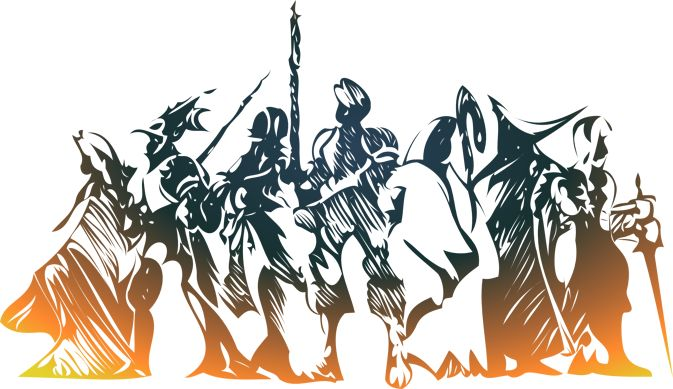
\includegraphics[width=0.9\columnwidth]{./art/images/tacticsog.jpg}
	\end{center}
}
%
\clearpage
\defaultgeometry
%
\ofsection{Gameplay}
%
\ofquote{"You want quiet, you better take the next train."\\}{Lightning}
%
\begin{center} 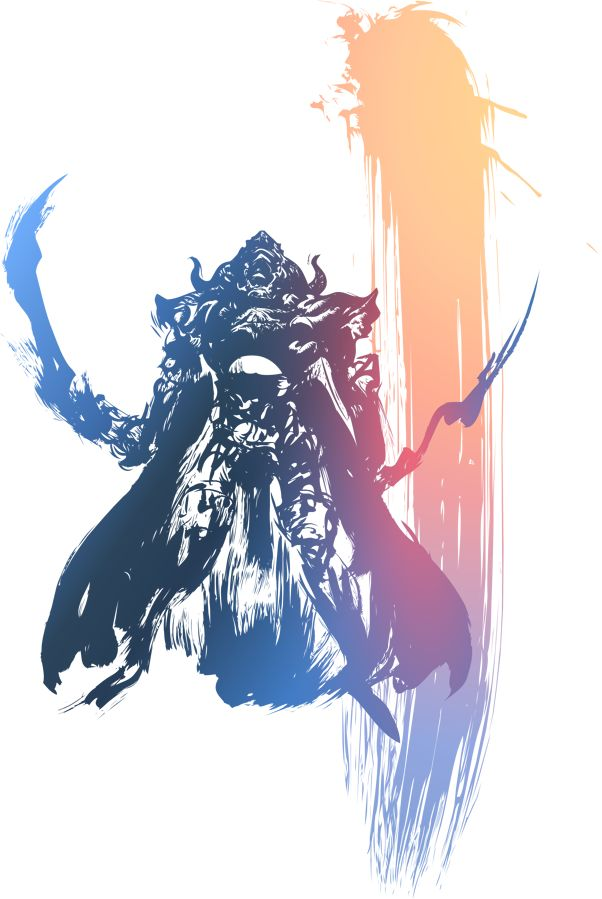
\includegraphics[width=\columnwidth]{./art/images/ff12.jpg} \end{center}
%
\accf{Final Fantasy} is a series of video games where each title features its unique story, world and characters.
Still they are part of the same series, not only due to recurring elements, but also because the stories focus on a group of heroes who face a great conflict.
\accf{Omega Fantasy} is a tabletop game that helps you to create Final Fantasy adventures with your friends and this release, named Omega~Fantasy~II, is an improved version of the original release.
To play, you only need dice, paper, pens, this book and at least one friend, but a group size of 4 to 6 is recommended.
To complete an adventure, your group needs to meet one or more times and play the game, each such gathering is called a \accf{Session}.
You do not necessarily have to meet in person, the game can also be played through online teleconferencing.
%
\ofpar
%
Choose one person to become the \accf{Game Master}~(shortened~\accf{GM}), who creates the game world and narrates the adventure by using the content and guidelines in this book.
During the game, he describes the environment to the players and how it reacts to their actions. 
The GM also takes the role of all non-player characters to narrate conversations and combat. 
Everyone else is a \accf{Player}, who creates and plays the game from the perspective of a \accf{Character} in the game world.
Player characters are the protagonists of the story who travel together as a \accf{Party} to explore the world, interact with people and fight against enemies. 
This book divided into three major sections: this first section explains the core rules and gameplay elements.
The second section details rules for creating and developing characters.
The final section focuses on the GM and offers a wide variety of guidelines and content for creating a game world. 
%
\vfill
%
\ofboxwithtitle{Example: Roleplaying\vspace*{0.15cm}}
{
	\newcommand{\nl}{\vspace{0.2cm}\\}
	\acc{Hironobu (Game Master):} You enter the Thunder Plains, which is a vast wasteland covered by thick fog and dark clouds.
	The locals have erected towers, that act as lightning rods, but you can see that lighting bolts often strike the ground in the open field.\nl
	\acc{Yoshinori (playing as Wakka):} We head north, not too near and not too far from the towers, ya?\nl
	\acc{Nobuo (playing as Rikku):} I wanna go home! I hate lightning! I hate thunder!\nl
	\acc{Tetsuya (playing as Auron):} This storm never stops. Better to cross quickly.\nl
	\acc{Hironobu (Game Master):} You can also see a small building nearby, that looks like an inn.\nl
	\acc{Nobuo (playing as Rikku):} Let’s go rest over there! Please? I'm too young to die!\nl
	\acc{Tetsuya (playing as Auron):} Fine, we rest. She is worse than the storm.
}
%
\vfill
%
Dice rolls are used to help decide the outcome of uncertain actions, but their exact nature depends on the context. 
This game only uses six-sided dice and we use \accf{d} shorthand to refer to such a die.
Furthermore, we use for example 4d to describe a roll of 4 dice, where the result is the sum of all rolled dice.
\accf{Checks} are the main tool to help the GM to decide and narrate the outcome of actions.
He can either ask players for checks or perform them himself in secret.
Checks are usually \accf{2d} rolls and higher numbers mean a better outcome for the roller. 
The minimum result to succeed is called Difficulty~(shortened \accf{DC}) and often has to be decided by the GM.
This DC should be based on the difficulty of the action and the proficiency of the actor.
Most DCs vary between 5 and 9, ones below this range are considered easy, while ones above it are very challenging.
%
\ofpar
%
Since checks are 2d rolls, the lowest and highest possible results are 2 and 12 respectively, which can be treated as unexpectedly good or bad, but still plausible outcomes.
A check can also have \accf{Advantage} or \accf{Disadvantage} when the circumstances have a substantial effect on the attempted action. 
In both cases, the check is made with 3d and with Advantage only the two highest and with Disadvantage only the two lowest dice are counted. 
Advantage and Disadvantage cancel each other out and do not stack.
%
%\ofpar
\clearpage
%
\ofboxwithtitle{Example: Advantage \& Disadvantage}
{
	Cloud meets Don Corneo in his mansion wearing a dress and make-up to convince him that he is a woman.
	The GM decides that this is a very difficult task (DC 10), because Cloud did not put much effort into his disguise. 
	But as the room is not well lit and the Don had a bit too much to drink, he also decides that the check has Advantage. 
	Cloud rolls 3d with the result [6,2,6] and since only the two highest dice count, he rolled the best possible outcome! 
	The GM decides that Don Corneo is not only convinced that Cloud is a woman, but he finds him so irresistible that he drags Cloud into his room for some time alone.
}
%
\ofpar
%
Another way to modify checks is through the use of \accf{Fortune Dice}.
At the start of each session, every player and the GM roll 1d and all results are written down and become the pool of Fortune Dice for this session.
During the session, after a player makes a roll, he or she can decide to remove one Fortune Die from the pool and use it to replace one die in the result of the roll.
However, the GM is also allowed to use Fortune Dice to modify the result of player rolls in the same manner.
This allows players to benefit from occasional strokes of luck or motivation while the GM can create moments of misfortune or complications.
In both cases, the person using the Fortune Die should try to give a narrative description of its effect.
Fortune Dice that are not used, are discarded at the end of each session.
%
\ofpar
%
\ofboxwithtitle{Example: Fortune Dice}
{
	Luneth explores the ancient Altar Cave. 
	As he walks towards a hole in the ground, the GM asks him for a DC~5 check to decide whether he can notice and avoid it.
	Luneth rolls [3, 4], which would pass the check.
	However, the GM decides to use a Fortune Die on his roll, the current pool of Fortune Dice includes \mbox{[1, 3, 3, 5]}.
	He removes the 1 from the pool and puts it in place of the 4 in Luneth's roll.  
	Accordingly, the roll is changed to [3, 1], which fails the check, and the remaining dice pool contains \mbox{[3, 3, 5]}.
	The GM describes this effect as follows: as he tries to carefully step around the hole, Luneth steps on a slippery rock, trips and falls into the hole.
	As a consequence, he finds himself an unknown and dangerous section of the cave and has find his way back to the exit.
}
%
\ofpar
%
\ofquote{"Why not? Nothing to lose but my life and I got that for free!"}{Setzer}\\\\
%
The party can explore the environment described by the GM at will.
They can look for specific things or wander around, but an appropriate amount of time passes while doing so.
The GM may draw a map of the party's current location as a visual aid. 
He is also free to impose checks on all exploration related actions, such as picking locks or detecting traps.
The party may go to sleep once per day to fully recover their HP and MP, even if unconscious.
To gain this benefit, they have to sleep in a comfortable place like an Inn or a Tent for multiple hours.
Throughout the adventure, the party will interact with other characters.
These non-player characters are voiced by the GM and accordingly the players talk from the perspective of their own characters.
To avoid confusion, it is important to clarify whether something you say is from the perspective of your character or from yours as player or GM.
During conversations, the GM may ask for checks, for example to decide whether an attempt to convince a character is successful.
%
\vfill
%
\ofquote{"You know what they say about the leading man, don't you? He never dies."}{Balthier}\\\\
%
Characters become stronger by gaining experience and we express the amount of experience a character has with \accf{Levels}.
Inexperienced adventurers start at Level 1 and can progress up to a maximum of Level 10 where they become renowned heroes. 
The GM decides when characters Level up, which we recommend for reaching adventure milestones.
Examples of milestones are important character development events, victories against powerful foes, or resolution of major conflicts. 
When going on dangerous adventures, \accf{Death} is always a real possibility, especially as a consequence of unwise decisions by the party. 
The adventure is officially over if all party members fall unconscious in battle, as this is usually followed by certain death. 
Characters may also die or leave the party under special circumstances in which case the GM takes control of him or her.
%
\ofpar
%
\ofboxwithtitle{Example: Experience \& Death}
{
	Kain betrays the party and joins their enemies. 
	He fights and defeats the rest of the party in combat, but chooses to let them stay alive.
	The GM takes control of Kain from now on, who leaves the party and becomes an antagonist.
	The party resolves to stop Kain's plan and his former player decides to create a new character that joins the party. 
	The GM rewards the party with a Level up for reaching a turning point in the adventure.
}
%
\vfill
%
Most adventures cover multiple sessions and sometimes a player might not be able to attend one.
In this case, the GM and the player can agree that his or her character leaves the party for the duration of that session to go on a \accf{Dispatch Mission}.
At the start of the next session, the character rejoins the party and the player explains what his or her character has tried to do during the previous session.
Then, the GM declares a DC for the Dispatch Mission and the player performs 3 checks with this DC.
If at least 2 out of the 3 checks succeed, then the mission was a success and if not, the character has failed in completing the mission.
%
\clearpage
\ofsubsection{Combat}
%
\ofquote{"Enough expository banter. It's time we fight like men. And ladies. And ladies who dress like men."\\}{Gilgamesh}\\
%
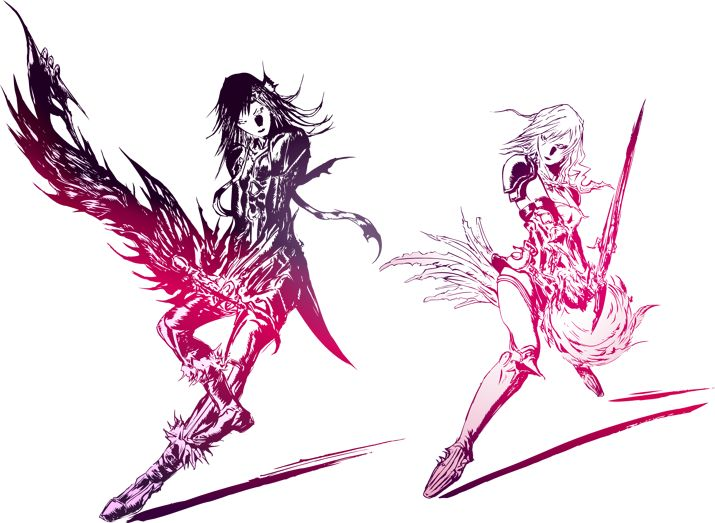
\includegraphics[width=\columnwidth]{./art/images/ff13-2.jpg}
%
\vfill
%
\accf{Combat} encounters are played out in a series of rounds (shortened~\accf{r}) and during a round, every combatant takes one turn.
At the start of the battle, both parties choose who takes the first turn in each round on their side and the GM the decides which side goes first.
Then, the opposing parties take alternating turns until every combatant has taken one and the round is finished.
The turn order for each side is decided as follows: at the end of their turns, every combatant chooses an ally who has not taken a turn in this round and should take the next one for their side.
If one side has more combatants, they can take consecutive turns at the end of the round until every participant has taken one.
Announce the start and end of each round to avoid confusion.
When a party ambushes the other before combat, the GM can decide that they gain a \accf{surprise round}.
In this case, only the surprising party acts in the first round before the battle continues as usual.
%
\vfill
%
Combat proficiencies are determined by the following 7 numerical \accf{attributes}.
Whenever a calculation results in a non-integer value, the result is always rounded down.
%
\ofgap
%
\ofmbox{\oficonhp\accf{Hit Points (HP)}} increase your durability. You have a maximum and a current number of HP, if your current HP falls to 0 you fall unconscious. \ofrow
\ofmbox{\oficonmp\accf{Mana Points (MP)}} are the resource required for using abilities such as Magic and Techs. Similar to HP, you have a maximum and a current number of MP. \ofrow
\ofmbox{\oficonstr\accf{Strength (STR)}} increases the damage dealt by your physical attacks. \ofrow
\ofmbox{\oficondef\accf{Defense (DEF)}} increases your resilience against physical damage. \ofrow
\ofmbox{\oficonmag\accf{Magic (MAG)}} increases the potency of your healing and attacking spells. \ofrow
\ofmbox{\oficonres\accf{Resistance (RES)}} increases your resilience against magical damage. \ofrow
\ofmbox{\oficonagi\accf{Agility (AGI)}} allows you to evade physical attacks and determines how quickly you can move.
%
\newpage
%
During your turn you can, in any order, move a distance of your AGI+1 units and take an action.
Below is a list of \accf{combat actions}, but the GM may allow any other action that can be completed in a similar amount of time:\ofgap
%
\ofmbox{\oficonattack\accf{Attack:}}
You attack an enemy with your weapon. 
He may evade by passing an \accf{evasion check} with a DC of 12 minus his AGI. 
If he fails the check, you reduce the target's HP by your weapon's DMG plus your STR.
If the evader rolls a 2, you make a \accf{critical hit}, doubling your usual damage. 
If he rolls a 12, not only does your Attack miss, but the evader makes an Attack action on you instead, which you cannot evade.\ofgap
%
\ofmbox{\oficonmagic\accf{Magic:}}
You cast a spell by spending MP, choosing a target within its range and concentrating for a duration.
While concentrating, you cannot take actions or evade. 
After the cast time is up, the spell's effect occurs on the target right \accf{before your turn} and cannot be evaded even if you are not in range anymore.
If the spell deals damage or restores HP, add your MAG to the amount.
Every spell's description has information on its cast time, MP cost, target, range and effect.\ofgap
%
\ofmbox{\oficontech\accf{Tech:}}
You use a non-magical ability. 
Techs are used the same way as magic, but their damage and healing is amplified by your STR instead of your MAG, 
except if their use already includes this bonus in another way, for example by involving an Attack.\ofgap
%
\ofmbox{\oficondefend\accf{Defend:}} All total damage that you receive by Attacks until your next turn is halved. \ofgap
%
\ofmbox{\oficonitem\accf{Item:}} You use an Item from your inventory on yourself or someone within 1u.\ofgap
%
\ofmbox{\oficonreequip\accf{Re-Equip:}} Swap a Materia or Equipment piece that you are wearing against one from your Inventory.\ofgap
%
\ofmbox{\oficondash\accf{Dash:}} Move to a location up to AGI +1 units away.\\\\
%
Apart from Magic and Techs, characters can also learn the following \accf{special abilities}: \ofrow
\ofmbox{\oficonpassive\accf{Passive:}} Effects that are permanently active. \ofgap
\ofmbox{\oficonreaction\accf{Reaction:}} Allow you to take certain actions on someone else's turn under specific conditions.
%
\vfill
%
\ofboxwithtitle{Example: Combat}
{
	Squall (4 DEF, 3 AGI, 1 RES) and Seifer (6 STR, 2 MAG) decide to duel.
	Both are wielding a gunblade~(1d DMG) and the GM decides that Seifer takes the first turn.
	He begins casting Firaga (6d DMG, 1r Time) by spending 12~MP, choosing Squall as its target and concentrating.
	Squall uses his turn to Defend.
	It's Seifer's turn again, so Firaga takes effect and Squall suffers \mbox{6d+2-1} damage. 
	Seifer can still take his turn, so he also Attacks. 
	Squall makes a \mbox{DC 12-3} evasion check, but by rolling [1, 1] he fails and suffers a Critical Hit! 
	Seifer hits him right above the nose with his blade, inflicting \mbox{1d+6-4} damage (Defend and Critical Hit cancel each other out) and leaving a scar.
}
%
\clearpage
%
\newcommand{\elemicon}[1]{\hspace*{-0.14cm}#1\hspace*{-0.14cm}}
All damage dealt has one of two basic types.
Unless specified otherwise, Attacks and Techs are of \accf{physical} type, while Magic and Items are of \accf{magical} type.
When you receive physical damage, subtract your DEF from the amount and when you receive magical damage, subtract your RES from the amount.
In addition, damage can have an elemental type to which combatants can have \accf{Weaknesses} or \accf{Resiliences}. 
When resilient, you only suffer half the usual damage and when weak, you suffer double the usual damage. 
Resilience and Weakness cancel each other out and do not stack.
The following elemental types exist: \elemicon{\fire}ire, \elemicon{\ice}ce, \elemicon{\lightning}ightning, W\elemicon{\water}ter, \elemicon{\earth}arth, \elemicon{\wind}ind, \elemicon{\holy}oly and \elemicon{\dark}ark.
%
\vfill
%
\accf{Units} (shortened \accf{u}) are the basis to measure distance, where 1u is roughly 1m or 3ft.
Characters usually occupy a circle of 1u in diameter in top view. 
Effect distances are described by their Range and Target.
\accf{Range} is the maximum distance between the center of the caster and the center of the effect. 
An effect with range Self is centered at the caster, and one with range Weapon has the same range as the used weapon.
\accf{Target} is the area of the effect as a maximum distance from its center. Unless stated otherwise, everyone fully or partially in the target area is affected, including allies.
An effect with target Single affects only a single entity.
The following illustration shows the use of a ranged effect in the normal case and with the two special target shapes Line and Front. 
%
\begin{figure}[h!]
		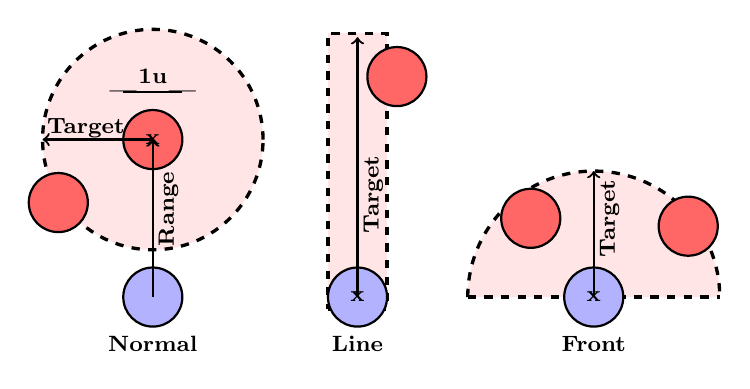
\begin{tikzpicture}[]
		\tikzstyle{test}=[thick, draw, circle, align=center]					
		%Normal
		\node[fill=blue!30!white, test,minimum size = 0.75cm](caster)at (0,0) {};
		\node[](t2)at (0,-0.6) {\bf\footnotesize Normal};
		\node[fill=red!10!white, test, very thick, dashed ,minimum size = 2.8cm](tarea)at (0,2) {};
		\node[fill=red!60!white, test,minimum size = 0.75cm](target)at (0,2) {};
		\node[fill=red!60!white, test,minimum size = 0.75cm](target)at (-1.2,1.2) {};
		\draw[thick, ->](0,0) -- node[] {}(0,2);
		\draw[thick, ->](0,2) -- node[] {}(-1.4, 2);
		\node[rotate=90](t1)at (0.2,1.12) {\bf\footnotesize Range};
		\node[](t2)at (-0.85,2.15) {\bf\footnotesize Target};
		\node[](t3)at (0,2) {\bf\footnotesize x};
		\node[](fi)at (-0.375,2.6) {\bf\footnotesize |};
		\node[](se)at (0.375,2.6) {\bf\footnotesize |};
		\draw[thick, -](0.375,2.6) -- node[] {}(-0.375,2.6);
		\node[](sca)at (0,2.8) {\bf\footnotesize 1u};		
		%Line
		\node[draw, fill=red!10!white, rectangle, very thick, dashed ,minimum height = 3.5cm, minimum width=0.75cm](tarea)at (2.6,1.6) {};
		\node[fill=blue!30!white, test,minimum size = 0.75cm](caster)at (2.6,0) {};
		\node[](t2)at (2.6,-0.6) {\bf\footnotesize Line};
		\node[fill=red!60!white, test,minimum size = 0.75cm](target)at (3.1,2.8) {};
		\draw[thick, ->](2.6,0) -- node[] {}(2.6,3.3);
		\node[rotate=90](t1)at (2.8,1.3) {\bf\footnotesize Target};
		\node[](t3)at (2.6,0) {\bf\footnotesize x};		
		%Front
		\draw[fill=red!10!white, test, very thick, dashed] (4,0) arc (180:0:1.6cm);
		\draw[dashed, very thick, -](4,0) -- node[] {}(7.2,0);
		\node[fill=blue!30!white, test,minimum size = 0.75cm](caster)at (5.6,0) {};
		\node[](t2)at (5.6,-0.6) {\bf\footnotesize Front};
		\draw[thick, ->](5.6,0) -- node[] {}(5.6,1.6);
		\node[rotate=90](t1)at (5.8,1) {\bf\footnotesize Target};
		\node[fill=red!60!white, test,minimum size = 0.75cm](target)at (4.8,1) {};
		\node[fill=red!60!white, test,minimum size = 0.75cm](target)at (6.8,0.9) {};
		\node[](t3)at (5.6,0) {\bf\footnotesize x};
		\end{tikzpicture}
\end{figure}
%
\vfill
%
\accf{Fields} are effects that occupy an area on the battlefield and cause harm to anyone inside.
They can be caused by abilities or natural causes such as steam or fog.
If at any point in your turn, you come into contact with a Field, you suffer its effect until the end of your turn.
Fields do not stack, when a new Field is created in the same area as an existing one, the previous Field is destroyed.
All Field effects are listed below.
%
\\\\
%
\oftable{p{0.17\columnwidth} p{0.77\columnwidth}}
{\accf{Field} & \accf{Effect}}
{
	Slow & You can only move half your usual distance.\ofrow
	Hot  & You receive fire damage equal to 10\% of your maximum HP.\ofrow
	Slippery & Make a DC~8 check and suffer Immobile upon failure.\ofrow
	Obscure & You suffer Blind.
}
%
\newpage
%
\accf{Status Effects} alter your the combat potency for a limited duration.
Combatants can suffer multiple different Status Effects at once, but applying the same one twice only refreshes its duration. 
They can also be \accf{Immune} to certain Status Effects, in which case they are not affected by them.
Also, if a combatant suffers two opposite Status Effects, for example Poison and Regen, they negate each other and are both removed.
Below is a list of all Status Effects. 
%
\vfill
%
\ofmbox{\oficonko\accrf{KO:}}
You are unconscious and your turns are skipped.
You suffer KO when your current HP drops to 0 and your HP cannot be increased until this status is removed.  
Immunity against KO only makes you immune against effects that cause it when above 0 HP.\ofgap
%
\ofmbox{\oficonblind\accrf{Blind:}} Whenever you Attack an enemy, he has Advantage on the evasion check. \ofgap
%
\ofmbox{\oficondestr\hspace*{-0.1cm}\oficondedef\hspace*{-0.1cm}\oficondemag\hspace*{-0.1cm}\oficonderes\accrf{DeATR:}} The according attribute is reduced by 1 plus half your current Level to a minimum 0. For example, DeSTR reduces your STR by 4 when you are Level 7.  \ofgap
%
\ofmbox{\oficonimmobile\accrf{Immobile:}} You are unable to move.\ofgap
%
\ofmbox{\oficonpoison\accrf{Poison:}} You take damage equal to 10\% of your maximum HP at the start of each of your turns, but cannot fall below 1 HP due to this effect.\ofgap
%
\ofmbox{\oficonsilence\accrf{Silence:}} You cannot begin casting Magic or using Techs, but you can still Attack.\ofgap
%
\ofmbox{\oficonslow\accrf{Slow:}} During your turn, you can either move or take an action but not both.\ofgap
%
\ofmbox{\oficonsleep\accrf{Sleep:}} You cannot move or take any action. This status is removed when you take any damage.\ofgap
%
\ofmbox{\oficonzombie\accrf{Zombie:}} All healing effects are reversed for you. Healing reduces your HP and effects that normally remove KO, inflict it to you instead.\ofgap
%	
\ofmbox{\oficonblink\accgf{Blink:}} Whenever you are targeted by an Attack, you have Advantage on the evasion check. \ofgap
%
\ofmbox{\oficonenstr\hspace*{-0.1cm}\oficonendef\hspace*{-0.1cm}\oficonenmag\hspace*{-0.1cm}\oficonenres\accgf{EnATR}} The according attribute is increased by by 1 plus half your current Level. For example, EnMAG increases your MAG by 2 when you are Level 3. \ofgap
%
\ofmbox{\oficonhaste\accgf{Haste:}} During your turn, you can either make an additional action or movement. \ofgap
%
\ofmbox{\oficonregen\accgf{Regen:}} You regain HP equal to 10\% of your maximum HP at the start of each of your turns.
%
\vfill
%
\ofboxwithtitle{Example: Status Effects}
{
	Noctis and Prompto fight Malboro. 
	The monster uses its Bad Breath ability to inflict multiple Status Effects.
	Prompto suffers Sleep and Poison.
	At the start of his turn he loses 3 HP (his maximum HP is 37) and he cannot move or take actions.
	Noctis suffers Silence and Blind.
	He cannot use abilities, so he tries to Attack Malboro. 
	The monster~(2~AGI) rolls [1,6,4] on the evasion check, barely passing the DC 12-2 check due to Advantage.
}
%
\clearpage

\ofsection{Jogadores}
%
\ofquote{"Eu sou O Basch fon Rosenburg!"\\}{Vaan}\\\\
%

\includegraphics[width=\columnwidth]{./art/images/ff10-2.jpg}
%
\vfill
%
Cada jogador cria um \accf{Personagem} que é um protagonista no mundo de jogo criado pelo MJ. 
Para criar um personagem de Nível 1, copie ou imprima a \accf{Ficha de Personagem} da próxima página. 
Ela permite a você acompanhar vários aspectos de seu personagem, há também um exemplo de ficha preenchida, como guia. 
Escolha o \accf{Nome} de seu personagem e faça uma descrição curta sobre ele. 
Resuma a \accf{História} dele e explique suas motivações para se juntar ao grupo, considerando que o mais provável é que essa seja a sua primeira aventura séria. 
Escolha então uma \accf{Profissão} como explicado abaixo. 
Por fim, a subseção de \accf{Equipamento} explica como você pode personalizar os equipamentos iniciais de seu personagem. 
A tabela à direita resume os benefícios fornecidos em Níveis subsequentes, todos explicados em detalhes dentro desta seção.
%
\vfill
%
A \accf{Profissão} de seu personagem determina a proficiência em combate dele, incluindo habilidades, atributos e especialidade com equipamentos. 
Todas as profissões são detalhadas nas suas descrições logo após as fichas de personagem. 
Imprima ou copie a descrição daquela escolhida por você para usar como uma segunda página de sua ficha de personagem.
Os atributos de seu personagem iniciam em 0 e aumentam ao progredir em uma profissão. 
A descrição de cada uma delas mostra os atributos e habilidades recebidos em cada Nível, assim como todos os tipos de equipamentos que o seu personagem usa. 
Quando o seu personagem alcança o Nível 3, você tem que decidir entre um ou dois \accf{Arquétipos}. 
Arquétipos representam diferentes especializações de uma profissão e fornecem habilidades e atributos adicionais.
%
\newpage
%
\ofboxwithtitle{Exemplo: Criação de Personagem}
{
	Nós criamos um personagem chamado Vaan, que tem 17 anos, um garoto humano, loiro e de aparência atlética. 
	Vaan é um órfão que se vira na cidade grande roubando e geralmente age como uma figura paterna para os outros órfãos. 
	Ele sonha em ter sua própria aeronave e um dia ser um pirata dos céus. 
	Nós escolhemos a profissão Ladrão e de sua tabela de atributos, nós determinamos o PV máximo~(20), PM máximo~(19) e AGI (4), todos os outros atributos começam em 0. 
	Nós também anotamos que ele aprende a técnica Roubar. 
	Por fim, de nossos 1500G iniciais, compramos uma faca de Mithril, um Colete de Mithril, uma Pena de Fênix e 2 poções, o que nos deixa com 300G sobrando.
}
%
\vfill
%
\oftable{p{0.25\columnwidth} p{0.7\columnwidth}}
{\accf{Nível} & \accf{Benefício ganho}}
{
	1 & Profissão, Equipamento iniciante \ofrow
	2 & Talento \ofrow
	3 & Arquétipo \ofrow
	4 & Quebra de Limite, Equipamento avançado\ofrow
	5 & Esper \ofrow
	6 & Especialização \ofrow
	7 & Especialização \ofrow
	8 & Especialização, Equipamento Especialista \ofrow
	9 & Especialização \ofrow
	10 & Especialização
}
%
\vfill
%
Nos Níveis marcados como \accf{Especialização}, escolha um dos seguintes benefícios para seu personagem.\ofrow
\ofbullet{No início de cada uma das sessões, adicione um 6 extra à reserva de Dados de Fortuna.}
\ofbullet{Ganhe uma segunda escolha de Esper.}
\ofbullet{Ganhe uma segunda escolha de Talento.}
\ofbullet{Ganhe um segundo Modo Limite, permite a você obter Pontos Limite de 2 fontes. Além disso, o alcance máximo de sua Quebra de Limite é aumentado em 2.}
\ofbullet{Ganhe acesso ao segundo Arquétipo de sua profissão. Você pode alternar entre os dois sempre que for dormir e seus atributos e habilidades mudam de acordo com aquele ativo no momento.}
\ofbullet{Ao usar Magia, Técnica ou habilidade de Reação de seu Arquétipo, o custo de seu PM é reduzido pela metade e você ganha 1 Ponto Limite.}
\ofbullet{Armas e armaduras ganham um espaço de Matéria adicional enquanto estiverem equipadas.}
\ofbullet{Ganhe a capacidade de equipar uma arma ou armadura adicional à sua escolha.}
\ofbullet{Escolha um bônus da lista a seguir. Não é possível escolher o mesmo benefício mais de uma vez: PV+5, PM+5, FOR+1, DEF+1, MAG+1, RES+1.}
%
\clearpage
%
\ofcs{}
%
\ofcs{
	name=Lightning,
	%
	description={%
		\vspace*{-0.5cm}
		\begin{multicols}{2}
			Idade: 21\\Raça: humano\\Cabelo: rosa\\Altura: 1.70m\\Destra\\ Determinada\\ Fria
			\columnbreak\vspace*{-1.7cm}\\
			\hspace*{-1cm}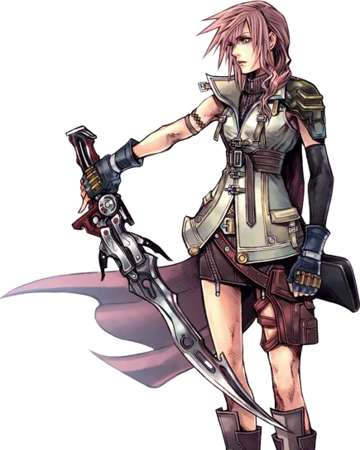
\includegraphics[width=1\columnwidth]{./art/charactersheets/claire.jpg}
		\end{multicols}
		\vspace*{-0.9cm}
	},
	%
	story={\\
		Meus pais morreram quando eu era jovem.
		Eu criei minha irmã, Serah, e me alistei no exército, no qual me tornei sargento.
		Mas agora Serah está em perigo, então eu tenho que deixar o exército e para encontrá-la. \\\\\\
		"Não é uma questão de ser capaz ou não.\\Há coisas na vida que você simplesmente faz."
	},
	% 
	hpcur=19, hpmax=91, mpcur=13, mpmax=85, agi=3, movement=4u, evasiondc=9, str=5, def=3, mag=7, res=2, 
	%
	level=8, job=Mago Vermelho, archetype=Devastador\phantom{1234567}, talent=Corporações Guardião,
	%
	abilities={Cura, Fogo, Nevasca, Raio, Cegueira,\\ Veneno, Esuna, AnuElemento},
	specials={Sobrepujar, Conjuração Rápida}, status={Cegueira (1r), AnDEF (2r)},
	%
	limitbreak=Raiara, limitmode=Bravura, limitpoints=\ofcslimitbarfilled, 
	limitdesc={Uma chuva de raios irrompe dos céus sobre um inimigo dentro de 5u e todos a 2u dele. Todos os alvos afetados sofrem 2d+8 de dano de raio.},
	%
	summon=Odin, summonused=yes, summonsupport={Realize um pequeno ritual para invocar o cavalo de Odin, Sleipnir.\\}, summonability={Um alvo no campo de batalha é afetado por KO se falhar num teste de DF~8 ou recebe dano igual a 3x seu nível se passar.},
	%
	weapon=Lâmina Pistola Dobrável, weaponbox=\ofcsweaponboxexpert, weaponeffect=Ataque à distância após a habilidade, weapontype= contra-ataque de 11 a 12 no teste de evasão, armor=Uniforme da Corporação Guardiã, armorbox=\ofcsarmorboxbeginner, armortype=DEF~+1, accessory1=Bracelete do Poder, accessory1effect=FOR~+1,
	%
	gil=2009, inventory={\\Faca de sobrevivência, 5x Granada, 5x Poção maior,\newline3x Remédio, 2x Pena da Fênix, 1x Elixir}
}
%
\clearpage
\ofsubsection{Jobs}
%
%
%
%
%
\ofjob{Bard}
{
	\ofquote{"Welcome to your doom, starring me!"\\}{Rikku}\\\\
	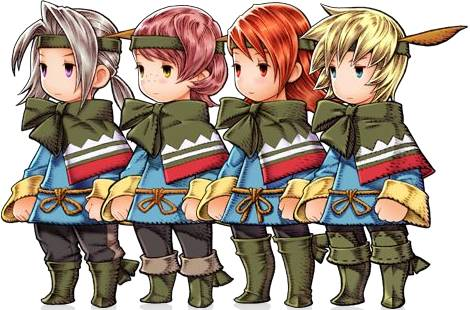
\includegraphics[width=\columnwidth]{./art/jobs/bard.jpg}\ofrow
	\accf{Bards} blur the lines between art and war.
	They can perform songs and dances that bestow powerful benefits for allies and vicious handicaps for enemies.
	Even though Bards are not the most powerful duelists, they can often turn the tide of a battle in unexpected ways.
}
{Dagger}{Light Armor or Robe}{
	Level 1: & HP~+19 & MP~+20 & AGI~+3 & RES~+1  \\
	Level 2: & HP~+10  & MP~+10 & DEF~+1  \\
	Level 3: & \multicolumn{3}{l}{Archetype Attribute Bonus} \\
	Level 4: & HP~+5  & MP~+10 & RES~+1 & DEF~+1 \\
	Level 5: & HP~+10 & MP~+5  & STR~+2 \\ 
	Level 6: & HP~+5  & MP~+10 & RES~+1 & DEF~+1 \\
	Level 7: & HP~+10 & MP~+10 & STR~+1 &  	  \\
	Level 8: & HP~+10  & MP~+10 & DEF~+1 \\
	Level 9: & HP~+10 & MP~+10 & STR~+1 \\
	Level 10: & HP~+5  & MP~+10 & RES~+1 & DEF~+1	
}{
	\ofjobtech{Cheer}{4}{0r}{1u}{Self}{Everyone in the target area can choose to either gain \mbox{EnSTR}, EnMAG, EnDEF or EnRES for 3 rounds.}{\enstr\enmag}{1}\ofabilitygap
	\ofjobtech{Improvise}{6}{0r}{Single}{5u}{Roll 1d. Based on the result, the target gains the following Status Effect for 3 rounds:\\ 1-EnDEF, 2-EnRES, 3-EnSTR, 4-Blink, 5-Regen, 6-Haste.}{\enndef\enres\enstr\blink\regen\haste}{2}\ofabilitygap
	\ofjobtech{Spotlight}{8}{0r}{2u}{Self}{You create an Obscure Field around yourself that follows you for 3 rounds, but does not affect you.}{}{4}\ofabilitygap
	\ofjobtech{Mighty March}{14}{0r}{2u}{Self}{You and all allies in the target area gain Haste and EnDEF for 2 rounds.}{\haste\enndef}{6}\ofabilitygap
	\ofjobtech{Charm}{15}{1r}{Single}{4u}{Choose an enemy as the target. He makes a DC~8 check and upon failure he immediately takes an extra turn following your command. The turn order is unchanged. Some enemies may be Immune to this effect.}{}{8}\ofabilitygap
	\ofjobtech{Mimic}{?}{0r}{?}{?}{You use an ability that was used by an ally or enemy on the battlefield since your last turn. In doing this, you have to respect the MP cost, cast time as well as the target and range of the copied ability.}{}{10}
}{
	\ofarchetypet{Dancer}
	{HP~+12 & MP~+8 & STR~+2 & DEF~+1}
	{\ofarchetypetecha{Blade Dance}{6}{0r}{Single}{1u}{Make an Attack on the target. Then you can immediately choose another target within 2u, dash towards him and make an Attack on him as well.}{}}
	{\ofspecial{Dress to Impress}{You can equip one additional Accessory. Also, for each equipped Accessory you can choose to gain either an additional DEF +1 or RES +1.}{5}{\oficonpassive}}	
	{\ofspecial{Dirty Dancing}{Whenever you successfully evade an Attack, you can immediately inflict one of the following Status Effects on the attacker for 3 rounds: Immobile, Poison, Blind.}{7}{\oficonreaction}}
	{\ofarchetypetechb{Slow Dance}{12}{0r}{2u}{Self}{You create a special Field around yourself that lasts for 3 rounds and simultaneously acts as a Slow Field and Hot Field. The Field moves together with you and it only affects enemies.}{}}
}{
	\ofarchetypet{Singer}
	{HP~+4 & MP~+16 & RES~+3}
	{\ofarchetypetecha{Requiem}{8}{0r}{Single}{4u}{The target makes a DC~8 check and upon failure he suffers dark damage equal to two times your current Level and Zombie for 3 rounds.}{\zombie\dark}}
	{\ofarchetypepassive{Encore}{Whenever you bestow one or more positive Status Effects on a target, additionally restore his HP by an amount equal to your current Level.}}
	{\ofarchetypereaction{Duet}{Whenever an ally within 1u of you performs an Attack or uses an ability on an enemy, you can immediately use any ability either on your ally or on the affected target if he is within range.}}
	{\ofarchetypetechb{Lullaby}{12}{0r}{2u}{5u}{All enemies in the target area make a DC~8 check and suffer 3d damage and Sleep for 3 rounds upon failure.}{\sleep}}
}
%
%
%
%
%
\ofjob{Black Mage}
{
	\ofquote{"You sure are a keen observer of the obvious, kupo!"\\}{Montblanc}\\\\
	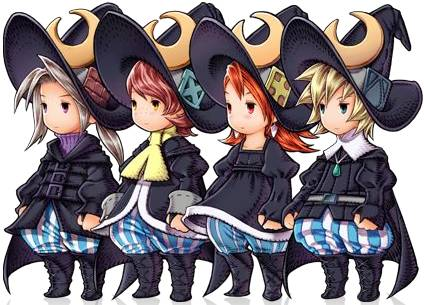
\includegraphics[width=\columnwidth]{./art/jobs/blackmage2.jpg}\ofrow
	\accf{Black Mages} are fragile in physical combat, but can wipe out enemies from great distances with powerful magic. 
	They assert great control over the battlefield and are difficult to ignore for enemies. 
}
{Rod}{Robe}{
	Level 1: & HP~+18 & MP~+26 & AGI~+2 & RES~+1  \\
	Level 2: & HP~+5  & MP~+10 & MAG~+1 & STR~+1  \\
	Level 3: & \multicolumn{3}{l}{Archetype Attribute Bonus} \\
	Level 4: & MP~+10 & RES~+1 & DEF~+1 & MAG~+1 	\\
	Level 5: & HP~+10 & MP~+10 & MAG~+1 		  \\
	Level 6: & HP~+5  & MP~+10 & RES~+1 & MAG~+1 \\
	Level 7: & HP~+5  & MP~+10 & MAG~+1 & RES~+1 \\
	Level 8: & HP~+5  & MP~+10 & RES~+1 & DEF~+1 \\
	Level 9: & HP~+5  & MP~+10 & RES~+1 & MAG~+1  \\
	Level 10: & HP~+10 & MP~+10 & MAG~+1		  
}{
	\ofjobspell{Fire}{4}{0r}{Single}{3u}{You deal 2d fire damage to the target.}{\fire}{1}\ofabilitygap
	\ofjobspell{Blizzard}{4}{0r}{Single}{3u}{You deal 2d ice damage to the target.}{\ice}{1}\ofabilitygap
	\ofjobspell{Thunder}{4}{0r}{Single}{3u}{You deal 2d lightning damage to the target.}{\lightning}{1}\ofabilitygap
	\ofjobspell{Blind}{6}{0r}{Single}{5u}{The target makes a DC 8 check and suffers Blind for 3 rounds upon failure.}{\blind}{2}\ofabilitygap
	\ofjobspell{Firaga}{12}{1r}{Single}{5u}{You deal 6d fire damage to the target.}{\fire}{6}\ofabilitygap
	\ofjobspell{Blizzaga}{12}{1r}{Single}{5u}{You deal 6d ice damage to the target.}{\ice}{6}\ofabilitygap
	\ofjobspell{Thundaga}{12}{1r}{Single}{5u}{You deal 6d lightning damage to the target.}{\lightning}{6}\ofabilitygap
	\ofjobspell{Flare}{25}{2r}{Single}{7u}{You deal 6d+45 damage to the target. The damage dealt ignores the target's RES.}{\fire}{8}\ofabilitygap
	\ofjobspell{Ultima}{30}{2r}{50u}{Self}{Deal 6d+40 dark damage to all enemies in the target area.}{\dark}{10}
}{
	\ofarchetypet{Geomancer}
	{HP~+14 & MP~+6 & DEF~+2 & RES~+1}
	{\ofarchetypespella{Bio}{8}{0r}{Single}{5u}{The target makes a DC 8 check and suffers 3d damage and Poison for 3 rounds upon failure.}{\poison}}
	{\ofarchetypepassive{Field Cast}{Whenever you cast a spell that deals fire, ice or lightning elemental damage, it also creates a Field around the target that reaches up to 2u and lasts for 1 round. The Field effect depends on the elemental type of the spell:\\ Fire - Hot Field, Ice - Slippery Field, Lightning - Slow Field.}}
	{\ofarchetypereaction{Gaia's Shield}{Whenever you suffer elemental damage, double your DEF and RES for calculating the damage received.}}
	{\ofarchetypespellb{Quake}{18}{1r}{3u}{10u}{Deal 6d+5 earth damage to everyone in the target area.}{\earth}}
}{
	\ofarchetypet{Scholar}
	{HP~+7 & MP~+18 & MAG~+2}
	{\ofarchetypespella{Thesis}{8}{0r}{Single}{5u}{Choose a type of action, for example Attack or Magic. If the target takes that type of action on his next turn, he suffers damage equal to 2 times your current Level and Immobile for 2 rounds.}{}}
	{\ofarchetypepassive{Analyze}{Whenever you deal magical damage, you can learn one of the following aspects about the target: Resiliences, Weaknesses, Immunities, current HP, current MP.}}
	{\ofarchetypereaction{Learn}{Whenever you are targeted by Magic, you can make a DC~8 check. If you succeed, you learn how to use the same spell. If you have already learned a spell in this way, you can choose to forget it to learn a new one.}}
	{\ofarchetypespellb{Specialize}{5}{0r}{Single}{5u}{The target chooses one of his known abilities. For the next 3 rounds, when the target uses that ability, its range is doubled and its MP cost is halved.}{\ko}}
}
%
%
%
%
%
\ofjob{Dragoon}
{
	\ofquote{"Confident bastard, aren't you?"\\}{Kain}\\\\
	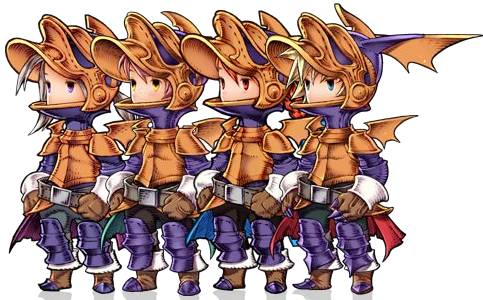
\includegraphics[width=\columnwidth]{./art/jobs/dragoon.jpg}\ofrow
	\accf{Dragoons} are masters of aerial combat, who strike their enemies with devastating attacks from the sky.
	They prefer spears as their weapon and have an affinity for the fire element. 
	Even though they are humanoid, it is said that Dragoons have the soul of a dragon.
}
{Spear}{Heavy Armor}{
	Level 1: & HP +23 & MP~+16 & AGI~+2,& STR~+1 \\
	Level 2: & HP~+10  & MP~+5 & STR~+1 & RES~+1 \\
	Level 3: & \multicolumn{3}{l}{Archetype Attribute Bonus} \\
	Level 4: & HP~+5  & MP~+10 & DEF~+2 &  	  \\
	Level 5: & HP~+10 & MP~+10 & STR~+1 & 		  \\ 
	Level 6: & HP~+10 & MP~+10 & RES~+1 		  \\
	Level 7: & HP~+10 & MP~+5  & STR~+1 & 	DEF~+1	  \\ 
	Level 8: & HP~+10 & MP~+10 & RES~+1 & 	 	  \\ 
	Level 9: & HP~+10  & MP~+10 & STR~+1 \\ 
	Level 10:& HP~+10  & RES~+1 & DEF~+2 
}{
	\ofjobtech{Jump}{4}{1r}{Single}{3u}{When you begin using this Tech, you jump 3u up into the air. After the cast time is up, you leap onto the target and make an Attack on him.}{}{1}\ofabilitygap
	\ofjobtech{Lancet}{3}{0r}{Single}{5u}{You deal damage to the target's HP and MP by an amount equal to your current Level and increase your own HP and MP by the same amount. This amount is not reduced by the target's DEF or RES.}{}{2}\ofabilitygap
	\ofjobtech{Double Jump}{8}{1r}{Single}{3u}{When you begin using this tech, you jump 3u up into the air. After the cast time is up, you leap onto the target and make an Attack on him. You can then leap to another location within 3u. If you land on another enemy you can make an Attack on him too.}{}{6}\ofabilitygap
	\ofjobtech{Roar}{8}{0r}{5u}{Self}{All enemies in the target area make a DC 9 check and suffer 2d damage and Immobile for 1 round upon failure.}{\immobile}{8}\ofabilitygap
	\ofjobtech{Highwind}{24}{1r}{Single}{Self}{For the next 3 rounds, you stay up to 3u in the air from where you can move your usual distance and perform one of the following 2 actions on each turn without additional MP cost or cast time:\\ 
		\acc{Lance Barrage:} make an Attack against a target within 10u. If you hit, you score a Critical Hit.\\
		\acc{Fire Blast:} choose a target within 10u. He and all enemies within 2u of him suffer 4d fire damage.
	}{\fire}{10}
}{
	\ofarchetypet{Dragon Knight}
	{HP~+8 & MP~+12 & STR~+1 & RES~+2}
	{\ofarchetypetecha{Fire Breath}{7}{0r}{3u (front)}{Self}{You deal 2d fire damage to everyone in the target area.}{\fire}}
	{\ofarchetypepassive{Flametongue}{You gain permanent Resilience against fire damage. Furthermore, whenever you deal physical damage to an enemy, you can choose to let the damage dealt be of magical and fire type instead.}}
	{\ofarchetypereaction{Dragonheart}{Whenever you deal or receive fire damage, you gain EnSTR until the end of your next turn.}}
	{\ofarchetypetechb{Dragon Dive}{16}{1r}{3u}{7u}{When you begin using this Tech, you jump 3u up into the air. After the cast time is up you leap onto the target and deal 4d fire damage to everyone in the target area except yourself. Also, you create Hot Field in the target area that lasts for 3 rounds but does not affect you.}{\fire}}
}{
	\ofarchetypet{Valkyrie}
	{HP~+13 & MP~+7 & STR~+2 & DEF~+1}
	{\ofarchetypetecha{Full Thrust}{6}{0r}{5u (line)}{Self}{You dash forward in an up to 5u long line. Make an Attack on everyone in the way by making one damage roll that is applied to all targets that fail to evade.}{}}
	{\ofarchetypepassive{Duelist}{As long as you are in combat within 3u of one enemy and there is noone else within 3u of you, the STR bonus added to your Attacks and Abilities is doubled.}}
	{\ofarchetypereaction{Arm's Length}{Whenever an enemy walks within 2u of you, he has to make a DC~7 check and upon failure he cannot move any further towards you on this turn.}}
	{\ofarchetypetechb{Revenge}{16}{0r}{Single}{1u}{Make an Attack on an enemy that has damaged you since your last turn. On hit, you inflict the damage that he dealt to you before instead of your usual damage.}{}}
}
%
%
%
%
%
\ofjob{Marksman}
{
	\ofquote{"I play the leading man; who else?"\\}{Balthier}\\\\
	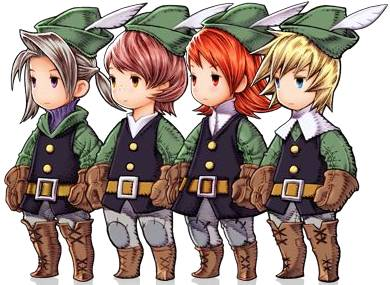
\includegraphics[width=\columnwidth]{./art/jobs/marksman.jpg}\ofrow
	\accf{Marksmen} are experts of all kinds of ranged weapons that strike from great distance. 
	Skilled Marksmen can see through their enemies, allowing them to know a target's strengths and weaknesses. 
	Therefore they can not only deal significant ranged damage, but also disable enemies with special techniques.
}
{Bow or Gun}{Light Armor}{
	Level 1: & HP +19 & MP~+17 & AGI~+2 & STR +1 \\
	Level 2: & HP~+10  & MP~+10 & DEF~+1 \\
	Level 3: & \multicolumn{3}{l}{Archetype Attribute Bonus}  \\
	Level 4: & HP~+5  & MP~+5  & STR~+2 & RES~+1 \\
	Level 5: & HP~+5  & MP~+10 & DEF~+1 & RES~+1  \\
	Level 6: & HP~+10 & MP~+10 & RES~+1 &        \\
	Level 7: & HP~+5  & MP~+10 & STR~+1 & RES~+1 \\
	Level 8: & HP~+10  & MP~+5 & DEF~+2 		  \\
	Level 9: & HP~+5  & MP~+10 & RES~+1 & STR~+1 \\
	Level 10:& HP~+10 & MP~+10 & STR~+1 &        
}{
	\ofjobtech{Libra}{4}{0r}{Single}{5u}{You analyse the target thoroughly and know his Resiliences, Weaknesses, Immunities, as well as his current HP and MP.}{}{1}\ofabilitygap
	\ofjobtech{Heavy Shot}{6}{0r}{Single}{Weapon}{Make an Attack on the target. If you hit, the damage dealt ignores the target's DEF.}{}{2}\ofabilitygap
	\ofjobtech{Fast Draw}{8}{0r}{Single}{Weapon}{You make an Attack after which you can immediately begin using another Ability in the same turn.}{}{4}\ofabilitygap
	\ofjobtech{Explosive Shot}{10}{0r}{2u}{Weapon}{Everyone in the target area suffers 3d fire damage. In addition, you create a Hot Field in the target area that lasts for 3 rounds.}{\fire}{6}\ofabilitygap
	\ofjobtech{Smoke Bomb}{10}{0r}{3u}{10u}{You create an Obscure Field in the target area that lasts for 3 rounds.}{}{8}\ofabilitygap
	\ofjobtech{Barrage}{24}{1r}{Single}{Self}{You gain Haste and EnSTR for 3 rounds. Also, all your Attacks which target a single enemy instead affect all enemies within 2u of the chosen target.
	}{\haste\enstr}{10}
}{
	\ofarchetypet{Ranger}
	{HP~+13 & MP~+12 & DEF~+2}
	{\ofarchetypetecha{Lay Trap}{5}{0r}{1u}{Self}{You set a trap where you are standing. An enemy that walks over it suffers damage equal to your current Level and Immobile for 1 round. The trap disappears once it is activated.}{\immobile}}
	{\ofarchetypepassive{Recoil}{Whenever you make a successful Attack, you can immediately move 1u in any direction.}}
	{\ofarchetypereaction{Magic Evade}{You can evade Magic by passing an evasion check. When you evade an Attack or Magic, you also regain an amount of MP equal to your current Level.}}
	{\ofarchetypetechb{Poison Ammo}{10}{0r}{Single}{Weapon}{Make an Attack on the target. If you hit, the damage dealt is magical and the target makes a DC 8 check. Upon failure, he suffers Poison, DeSTR and DeDEF for 3 rounds.}{\poison\destr\dedef}}
}{
	\ofarchetypet{Sniper}
	{HP~+5 & MP~+15 & STR~+3}
	{\ofarchetypetecha{Pierceshot}{6}{0r}{10u (line)}{Self}{Make an Attack against all targets in a line, by making one damage roll that applies to everyone that fails to evade.}{}}
	{\ofarchetypepassive{Concentrate}{Whenever you Attack an enemy, he has Disadvantage on the evasion check.}}
	{\ofarchetypereaction{Camouflage}{Whenever you end a turn in which you have not moved, you gain Blink until the start of your next turn.}}
	{\ofarchetypetechb{Aim}{8}{0r}{Single}{Weapon}{Make an Attack on the target and choose one of the following spots to inflict an additional effect if you hit:\\ \acc{Head:} the target's evasion DC is reduced by 2, but if you hit you score a Critical Hit.\\ \acc{Heart:} the target's MP is reduced by same amount as HP.\\ \acc{Leg:} the target suffers Immobile for 1 round.}{\immobile}}
}
%
%
%
%
%
\ofjob{Monk}
{
	\ofquote{"Now I know why I have these stupid muscles!"\\}{Sabin}\\\\
	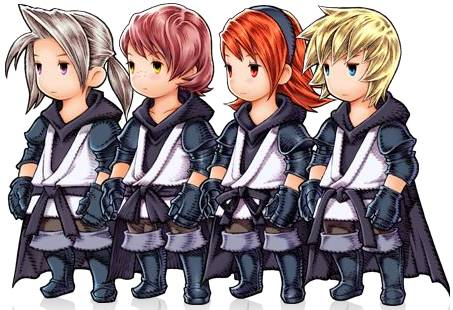
\includegraphics[width=\columnwidth]{./art/jobs/monk2.jpg}\ofrow
	\accf{Monks} are adept melee fighters that posses a deadly combination of strength and technique.
	While they do not have expertise in using magic, Monks can produce similar effects by tapping into their inner life force. 
}
{None}{Light Armor}{
	Level 1: & HP +20 & MP~+16 & AGI~+4 & \\
	Level 2: & HP~+10 & MP~+5  & STR~+2 & \\
	Level 3: & \multicolumn{3}{l}{Archetype Attribute Bonus} \\
	Level 4: & HP~+5  & MP~+10 & STR~+1 & RES~+1 \\
	Level 5: & HP~+10  & MP~+5 & DEF~+1 & STR~+1 \\
	Level 6: & HP~+10 & MP~+5  & STR~+1 & RES~+1 \\
	Level 7: & HP~+10 & MP~+5  & STR~+1 & DEF~+1 \\ 
	Level 8: & HP~+10 & MP~+5  & DEF~+2 &        \\
	Level 9: & HP~+5  & MP~+10 & STR~+1 & RES~+1 \\ 
	Level 10: & HP~+10 & MP~+10 & DEF~+1 &        \\ 
}{
	\ofjobpassive{Brawler}{In combat, you can use your bare fists as your weapon. They have the same DMG as weapons of the highest equipment rank that you can use. In addition, you can carry a third Accessory in place of your weapon slot and you gain STR +1 for every equipped Accessory. You may also slot materia onto the Accessory that you are carrying in place of a weapon.}{1}\ofabilitygap
	\ofjobtech{Kick}{4}{0r}{1u}{Self}{You make an Attack against all enemies within 1u of you, by making one damage roll that applies to all affected targets that fail to evade. All targets that fail to evade are also knocked back by 1u.}{}{2}\ofabilitygap
	\ofjobtech{Aurablast}{6}{0r}{Single}{3u}{You deal an amount of magical damage equal to your current Level to the target.}{}{4}\ofabilitygap
	\ofjobtech{Pummel}{8}{0r}{Single}{1u}{You make 2 consecutive Attacks against the target.}{}{6}\ofabilitygap
	\ofjobtech{Blitz}{3}{0r}{Single}{Self}{You use two different Techs consecutively in the same turn. In doing this, you have to respect additional MP costs and cast times of both Techs.}{}{8}\ofabilitygap
	\ofjobtech{Final Heaven}{22}{0r}{Single}{1u}{You deal 6d damage to the target and knock him back by 5u. If he hits a wall or a similarly solid object in doing so, you deal another 3d damage to him.}{}{10}
}{
	\ofarchetypet{Black Belt}
	{HP~+17 & MP~+8 & STR~+2}
	{\ofarchetypetecha{Bonecrusher}{6}{0r}{Single}{1u}{Make an Attack against the target. On hit, the target makes a DC~8 check and suffers Slow for 1 round upon failure.}{\slow}}
	{\ofarchetypepassive{Unscarred}{As long as your current HP is equal to your maximum HP, the STR bonus that is added to the damage dealt by your Attacks is doubled.}}
	{\ofarchetypereaction{Strikeback}{When you successfully evade an Attack by an enemy, you immediately make an Attack on him, if he is within range.}}
	{\ofarchetypetechb{Meteor Strike}{14}{0r}{Single}{1u}{You slam the target into the ground dealing 5d damage. In doing this, you can also leap to a location of your choice within 3u.}{}}
}{
	\ofarchetypet{Templar}
	{HP~+4 & MP~+16 & DEF~+1 & RES~+2}
	{\ofarchetypetecha{Chakra}{6}{1r}{Single}{Self}{You regain an amount of HP equal to your current Level and recover from one Status Effect that you are currently suffering.}{}}
	{\ofarchetypepassive{Lifestream}{If you do not have enough MP to use an ability you can instead choose to reduce your HP by the amount of its MP cost in order to use it.}}
	{\ofarchetypereaction{Replenish MP}{Whenever you suffer physical damage, you regain an amount of MP equal to half your current Level.}}
	{\ofarchetypetechb{Revive}{14}{1r}{Single}{1u}{You remove KO from the target and increase his HP by~1.}{\ko}}
}
%
%
%
%
%
\ofjob{Red Mage}
{
	\ofquote{"Oh, I’ll show you how lightning strikes."\\}{Lightning}\\\\
	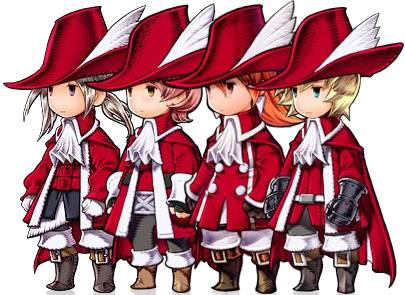
\includegraphics[width=\columnwidth]{./art/jobs/redmage.jpg}\ofrow
	\accf{Red Mages} are very versatile and possess a wide variety of abilities, but can also hold their own in melee combat. 
}
{Rod or Sword}{Light Armor or Robe}{
	Level 1: & HP~+20 & MP~+21 & AGI~+3 & STR +1 \\
	Level 2: & HP~+5  & MP~+10 & MAG~+1 & DEF~+1 \\
	Level 3: & \multicolumn{3}{l}{Archetype Attribute Bonus}   \\
	Level 4: & HP~+10 & MP~+5  & STR~+1 & RES~+1 \\   
	Level 5: & HP~+5  & MP~+10 & MAG~+2 & 		  \\ 
	Level 6: & HP~+5 & MP~+10  & STR~+1 &	MAG~+1 \\ 
	Level 7: & HP~+10  & MP~+10 & DEF~+1 \\ 
	Level 8: & HP~+10 & MP~+5  & STR~+1 & MAG~+1 \\ 
	Level 9: & HP~+5  & MP~+10 & RES~+2 \\ 
	Level 10: & HP~+10 & MP~+10 & STR~+1 		  
}{	
	\ofjobspell{Fire}{4}{0r}{Single}{3u}{You deal 2d fire damage to the target.}{\fire}{1}\ofabilitygap
	\ofjobspell{Blizzard}{4}{0r}{Single}{3u}{You deal 2d ice damage to the target.}{\ice}{1}\ofabilitygap
	\ofjobspell{Thunder}{4}{0r}{Single}{3u}{You deal 2d lightning damage to the target.}{\lightning}{1}\ofabilitygap
	\ofjobspell{Regen}{6}{0r}{Single}{5u}{The target gains Regen for 3 rounds.}{}{2}\ofabilitygap
	\ofjobspell{Blind}{6}{0r}{Single}{5u}{The target makes a DC~8 check and suffers Blind for 3 rounds upon failure.}{\blind}{4}\ofabilitygap	
	\ofjobspell{Vox}{6}{0r}{Single}{5u}{Remove one Status Effects except KO from the target. Also, the target becomes Immune to that Status Effect for 5 rounds.}{}{6}\ofabilitygap
	\ofjobspell{Imperil}{8}{0r}{Single}{5u}{The target suffers DeDEF and DeRES for 3 rounds.}{}{8}\ofabilitygap
	\ofjobspell{Wall}{8}{0r}{Single}{5u}{The target gains EnDEF and EnRES for 3 rounds.}{}{8}\ofabilitygap
	\ofjobspell{Dualcast}{2}{0r}{Single}{Self}{You begin casting two spells of your choice simultaneously, but need to spend the necessary MP for both.}{}{10}
}{
	\ofarchetypet{Ravager}
	{HP~+6 & MP~+14 & MAG~+2 & RES~+1}
	{\ofarchetypespella{Osmosis}{0}{0r}{Single}{5u}{You regain MP equal to your MAG and the target's MP is reduced by the same amount.}{}}
	{\ofarchetypepassive{Overwhelm}{When you inflict elemental damage, the target gains a weakness against that type until the end of your next turn. If he has a Resilience against it, that is negated instead.}}
	{\ofarchetypereaction{Swiftcast}{Once per round, right after an enemy within 5u uses an action, you can immediately cast a spell on him.}}
	{\ofarchetypespellb{NulElement}{10}{0r}{Single}{5u}{Choose an element (e.g. fire). The target does not suffer any damage of the chosen element for 3 rounds.}{}}
}{
	\ofarchetypet{Spellblade}
	{HP~+14 & MP~+6 & STR~+2 & DEF~+1}
	{\ofarchetypetecha{Elemental Strike}{6}{0r}{Single}{1u}{Choose an element (e.g. fire) and make an Attack. If you hit, the damage is of magical type with the chosen element and you also add your MAG to the damage dealt.}{}}
	{\ofarchetypepassive{Magic Weapon}{Whenever you cast Magic, you can choose to store the spell inside your weapon. In this case, the spell's MP cost is halved. All stored spells take effect together with your next successful Attack and you can chose targets within their range including yourself. You cannot store more than two spells at once inside your weapon.}}
	{\ofarchetypereaction{Mana Shield}{Whenever your HP is reduced, you can instead choose to reduce your MP by the same amount.}}
	{\ofarchetypetechb{Magic Barrier}{10}{0r}{Single}{5u}{For the next 3 rounds, the target can evade the effect of spells and techs by passing an evasion check.}{}}
}
%
%
%
%
%
\ofjob{Sentinel}
{
	\ofquote{"Allow me to shatter your delusions of grandeur."\\}{Beatrix}\\\\
	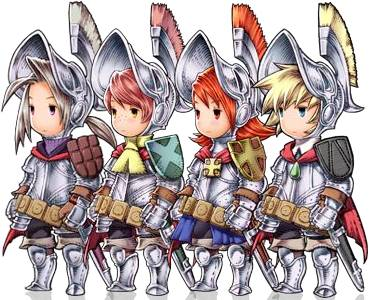
\includegraphics[width=\columnwidth]{./art/jobs/sentinel.jpg}\ofrow
	\accf{Sentinels} are masters of defensive combat who will rarely fall in a battle.  
	Their special abilities allow them to not only withstand incredible amounts of damage, but also provide protection to their allies.
	A capable Sentinel is often the last thing standing between the party and certain death.
}
{Sword}{Heavy Armor}{
	Level 1: & HP~+27 & MP~+16 & AGI~+3 & STR~+1  \\
	Level 2: & HP~+10 & MP~+10 & DEF~+1 & RES~+1 \\
	Level 3: & \multicolumn{3}{l}{Archetype Attribute Bonus} \\
	Level 4: & HP~+10 & MP~+5  &  DEF~+1 & STR~+1 \\ 
	Level 5: & HP~+10 & MP~+5  & RES~+1 & DEF~+1 \\ 
	Level 6: & HP~+10 & MP~+10 & STR +1 &        \\
	Level 7: & HP~+10 & MP~+5  & DEF +2 &        \\
	Level 8: & HP~+10 & MP~+5  & STR +1 & DEF~+1 \\
	Level 9: & HP~+10 & MP~+10 & STR +1 &        \\
	Level 10: & HP~+10  & MP~+10 & DEF +1 
}{
	\ofjobtech{Guard}{3}{0r}{Single}{Self}{You gain EnDEF until the end of your next turn.}{\enndef}{1}\ofabilitygap
	\ofjobtech{First Aid}{6}{1r}{Single}{1u}{%
		When you begin using this ability, the target regains an amount of HP equal to your current Level. After the cast time is up, if you have received no damage since casting and if the target is still in range, he additionally gains EnDEF and Haste for 1 round.}{}{2}\ofabilitygap
	\ofjobtech{Threaten}{6}{0r}{Single}{5u}{The target makes a DC 8 check and suffers Immobile for 3 rounds upon failure.}{\immobile}{4}\ofabilitygap
	\ofjobtech{Mediguard}{9}{0r}{Single}{Self}{You gain EnDEF and Regen for 3 rounds.}{\enndef}{6}\ofabilitygap
	\ofjobtech{Defensive Formation}{10}{0r}{2u}{Self}{You and all allies within the target area gain Blink for 2 rounds.}{\blink}{8}\ofabilitygap
	\ofjobtech{Mighty Guard}{26}{1r}{Single}{Self}{For the next 3 rounds, you gain Resilience against all physical and magical damage.}{}{10}
}{
	\ofarchetypet{Defender}
	{HP~+17 & MP~+3 & STR~+2 & DEF~+1}
	{\ofarchetypetecha{Powerbreak}{6}{0r}{Single}{1u}{Make an Attack on the target. If you hit, he suffers DeSTR and DeMAG for 2 rounds on top of the damage dealt.}{\destr \demag}}
	{\ofarchetypepassive{Provoke}{Whenever you successfully Attack an enemy, you can try to provoke him. If you do so, he has to make a DC~8 check and upon failure he has to target you with an action on his next turn if possible.}}
	{\ofarchetypereaction{Block}{Whenever an enemy within 2u of you tries to move away from you, he has make a DC 8 check. Upon failure, he suffers Immobile until the start of his next turn, preventing him from moving any further on this turn.}}
	{\ofarchetypetechb{Vengeance}{14}{0r}{Single}{1u}{The target suffers damage equal to half the difference between your current and your maximum HP.}{}}
}{
	\ofarchetypet{Paladin}
	{HP~+10 & MP~+15 & RES~+2}
	{\ofarchetypetecha{Earth Wall}{8}{0r}{3u (line)}{8u}{You create a 3u tall and wide wall of earth that blocks the path. The wall breaks down after 3 rounds or upon suffering a total of 20 damage. You cannot use this ability if a previous wall still exists.}{}}
	{\ofarchetypepassive{Holy Guard}{As long as there is at least one ally within 1u of you, you and all allies within 1u gain EnRES.}}
	{\ofarchetypereaction{Cover}{Whenever an ally within 1u of you receives physical damage, you can decide to direct half of the total damage dealt on yourself instead of onto your ally.}}
	{\ofarchetypetechb{Astra}{10}{0r}{Single}{5u}{For the next 3 rounds, the target gains EnRES and becomes Immune to all Status Effects.}{\enres}}
}
%
%
%
%
%
\ofjob{Summoner}
{
	\ofquote{"I don’t like your plan. It sucks."\\}{Yuna}\ofrow
	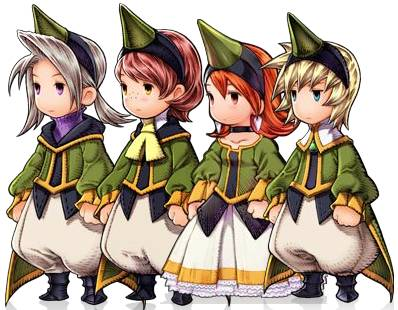
\includegraphics[width=\columnwidth]{./art/jobs/summoner.jpg}\ofrow
	Most powerful heroes are able to call creatures, but the bonds created \accf{Summoners} are far stronger allowing them
	manifest summons for a longer time to fight alongside them on the battlefield.
}
{Rod or Staff}{Robe}{
	Level 1: & HP +16 & MP~+24 & AGI~+2 & STR~+1 \\ 
	Level 2: & HP~+5  & MP~+10 & RES~+1 & MAG~+1 \\ 
	Level 3: & \multicolumn{3}{l}{Archetype Attribute Bonus}   \\
	Level 4: & HP~+5  & MP~+10 & RES~+1 & DEF~+1 \\ 
	Level 5: & HP~+5 & MP~+5  & RES~+2 & MAG~+1 \\  
	Level 6: & HP~+10 & MP~+10 & DEF~+1 \\  
	Level 7: & HP~+5 & MP~+10 & RES~+1 &  MAG~+1      \\  
	Level 8: & HP~+5 & MP~+10 & DEF~+1 &		  \\  
	Level 9: & HP~+10 & MP~+5  & MAG~+1 & RES~+1 \\  
	Level 10: & HP~+10 & MP~+10 & STR~+1 &        	  
}{
	\ofjobspell{Summon}{8}{1r}{1u}{1u}{
		You manifest a creature, that you have the ability to summon, on the battlefield.  
		In combat, summons take their turn right after yours, following your command.
		They are dismissed when they suffer KO, when you summon again or at the end of the battle.
		The HP \& MP of a summon is the same as when it was dismissed, if it suffered KO, it is summoned with 1 HP.
		Summons fully recover their HP \& MP when you go to sleep.
		Your summons level up with you where gain the same attribute increases as you.
		All summons and their abilities are shown on the next page.
	}{}{1}\ofabilitygap
	\ofjobpassive{Summon: Carbuncle}{You gain the ability to summon \acc{Carbuncle}.}{1}\ofabilitygap
	\ofjobspell{Image}{6}{0r}{Single}{5u}{The target gains Blink for 3 rounds.}{\blink}{2}\ofabilitygap
	\ofjobspell{Dispel}{10}{0r}{Single}{5u}{All Resiliences and active beneficial Status Effects of the target are removed for 3 rounds.}{}{6}\ofabilitygap
	\ofjobpassive{Summon: Bahamut}{You gain the ability to summon \acc{Bahamut}.}{8}\ofabilitygap
	\ofjobspell{Final Summon}{16}{1r}{1u}{1u}{
		Inflict KO to a currently summoned creature to summon a new one.
		The new summon gains EnSTR, EnDEF, EnMAG, EnRES and Regen until the end of the battle.
	}{}{10}
}{
	\ofarchetypet{Devout}
	{HP~+7 & MP~+13 & STR~+1 & RES~+2}
	{\ofarchetypespella{Pray}{6}{0r}{1u}{Self}{You and all allies in the target area regain 2d HP.}{}}
	{\ofarchetypepassive{Inferno}{You gain the ability to summon \acc{Ifrit} and permanent Resilience against fire damage. Also, whenever one of your summons deals damage, add your STR and MAG to the summon's for calculating the total damage dealt.}}
	{\ofarchetypereaction{Blood Pact}{Whenever your currently active summon receives any damage, you can redirect half of the total damage dealt to your own HP.}}
	{\ofarchetypespellb{Healing Wind}{14}{0r}{5u (line)}{Self}{You and all allies in the target area regain 4d HP.}{}}
}{
	\ofarchetypet{Evoker}
	{HP~+12 & MP~+8 & MAG~+2 & DEF~+1}
	{\ofarchetypespella{Aero}{6}{0r}{Single}{4u}{You deal 2d wind damage to the target.}{\wind} \ofabilitygap	\ofarchetypespella{Water}{6}{0r}{Single}{4u}{You deal 2d water damage to the target.}{\water}}
	{\ofarchetypepassive{Ice Queen}{You gain the ability to summon \acc{Shiva} and permanent Resilience against ice damage. Also, you can use all spells and techs known by your currently active summon.}}
	{\ofarchetypereaction{Absorb Summon}{Whenever one of your summons suffers KO in combat, you regain an amount of HP and MP equal to 2 times your current Level, as well as EnMAG for 3 rounds.}}
	{\ofarchetypespellb{Aeroga}{14}{1r}{Single}{6u}{You deal 6d wind damage to the target.}{\wind} \ofabilitygap \ofarchetypespellb{Waterga}{14}{1r}{Single}{6u}{You deal 6d water damage to the target.}{\water}}
}
%
\clearpage
%
\ofmonster{Carbuncle}{1}{
\includegraphics[width=0.25\columnwidth]{./art/jobs/carbuncle.jpg}}
{
	HP: & \hfill 10 & MP: & \hfill 12\\
	STR: & \hfill 1 & DEF: & \hfill 1 \\
	MAG: & \hfill 0 & RES: & \hfill 1 \\
	AGI: & \hfill 3 & Size: & \hfill S\\
}
{\accf{Bite}: 1d DMG (increased to 2d at Level 5)}
{
	\mspell{Thunder \hfill \accf{Level 2}}{4}{0r}{Single}{3u}{You deal 2d lightning damage to the target.}{}
	\mspell{Reflect \hfill \accf{Level 4}}{10}{0r}{Single}{3u}{The target gains a shield that reflects the next spell that targets them back to its caster.}{}
	\mspell{Flash \hfill \accf{Level 7}}{8}{0r}{3u (front)}{Self}{All enemies in the target area make a DC~8 check and suffer Blind for 3 rounds upon failure.}{}
	\mspell{Wall \hfill \accf{Level 8}}{8}{0r}{Single}{5u}{The target gains EnDEF and EnRES for 3 rounds.}{}
	\mspell{Ruby Light \hfill \accf{Level 10}}{24}{1r}{2u}{8u}{All allies in the target area gain Regen for 3 rounds and a shield that reflects the next spell that targets them back to its caster.}{}
}
%
\vspace*{1.8cm}\\
%
\ofmonster{Ifrit}{5}{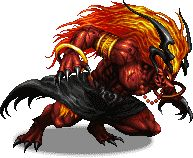
\includegraphics[width=0.28\columnwidth]{./art/jobs/ifrit.jpg}}
{
	HP: & \hfill 30 & MP: & \hfill 25\\
	STR: & \hfill 3 & DEF: & \hfill 2 \\
	MAG: & \hfill 1 & RES: & \hfill 0 \\
	AGI: & \hfill 3 & Size: & \hfill M\\
}
{
	\accf{Claw}: 2d DMG  (increased to 3d at Level 8)\\
	\accf{Resilience}:\fire \hfill \accf{Weakness:}\ice
}
{	
	\mspell{Fire \hfill \accf{Level 5}}{4}{0r}{Single}{3u}{You deal 2d fire damage to the target.}{\fire}	
	\mtech{Burning Strike \hfill \accf{Level 5}}{5}{0r}{Single}{1u}{Make an Attack on the target. If you hit, he additionally suffers 2d fire damage.}{}	
	\mtech{Mad Rush \hfill \accf{Level 7}}{8}{0r}{5u (line)}{Self}{You dash forward in an up to 5u long line and deal 4d damage to everyone in the way.}{}	
	\mspell{Firaga \hfill \accf{Level 8}}{12}{1r}{Single}{5u}{You deal 6d fire damage to the target.}{\fire}
	\mtech{Hellfire \hfill \accf{Level 10}}{20}{0r}{2u}{Self}{All enemies in the target area suffer 6d+10 fire damage.}{\fire}	
}
%
\newpage
%
\ofmonster{Bahamut}{9}{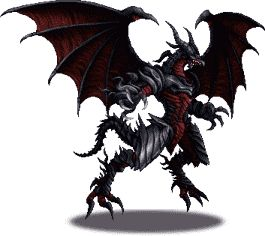
\includegraphics[width=0.3\columnwidth]{./art/jobs/bahamut.jpg}}
{
	HP: & \hfill 60 & MP: & \hfill 80\\
	STR: & \hfill 5 & DEF: & \hfill 4 \\
	MAG: & \hfill 4 & RES: & \hfill 4 \\
	AGI: & \hfill 3 & Size: & \hfill L\\
}
{
	\accf{Claw}: 3d DMG\\
	\accf{Immune}: All Status Effects \hfill \accf{Resilience:}\dark\fire
}
{
	\mreaction{Final Attack}{If you are about to fall to 0 HP you may use one of your abilities without cost or cast time before falling KO.}
	\mtech{Impulse \hfill \accf{Level 9}}{12}{0r}{3u}{Self}{All enemies in the target area suffer 3d dark damage.}{\dark}{}	
	\mtech{Obliterating Breath \hfill \accf{Level 9}}{14}{0r}{3u (front)}{3u}{Everyone in the target area makes a DC 8 check and suffers 3d damage as well as Poison and Blind for 3 rounds upon failure.}{\poison \blind}{}
	\mspell{Megaflare \hfill \accf{Level 10}}{25}{2r}{2u}{10u}{You deal 6d+40 damage to all enemies in the target area. The damage dealt ignores the target's RES.}{\fire}
}
%
\vfill
%
\ofmonster{Shiva}{5}{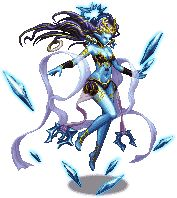
\includegraphics[width=0.23\columnwidth]{./art/jobs/shiva.jpg}}
{
	HP: & \hfill 25 & MP: & \hfill 45\\
	STR: & \hfill 2 & DEF: & \hfill 1 \\
	MAG: & \hfill 3 & RES: & \hfill 4 \\
	AGI: & \hfill 2 & Size: & \hfill M\\
}
{
	\accf{Icicle}: 2d DMG, 2u Range  (increased to 3d at Level 8)\\
	\accf{Resilience}:\ice \hspace*{\fill} \accf{Weakness:}\fire
}
{	
	\mspell{Blizzard \hfill \accf{Level 5}}{4}{0r}{Single}{3u}{You deal 2d ice damage to the target.}{}
	\mspell{Deprotect \hfill \accf{Level 5}}{5}{0r}{Single}{5u}{The target suffers DeDEF for 3 rounds.}{\dedef}
	\mspell{Deshell \hfill \accf{Level 5}}{5}{0r}{Single}{5u}{The target suffers DeRES for 3 rounds.}{\deres}
	\mspell{Ice Wall \hfill \accf{Level 7}}{12}{0r}{3u (line)}{5u}{You create a 3u tall and wide wall of ice that blocks the path for 3 rounds. You cannot use this ability again as long as the previous wall still stands.}{}
	\mspell{Blizzaga \hfill \accf{Level 8}}{12}{1r}{Single}{5u}{You deal 6d ice damage to the target.}{\ice}
	\mspell{Diamond Dust \hfill \accf{Level 10}}{20}{0r}{3u (front)}{Self}{All enemies in the target area suffer 6d ice damage and Immobile for 1 round.}{\ice\immobile}		
}
\clearpage
%
%
%
%
%
\ofjob{Thief}
{
	\ofquote{"I PREFER the term ”treasure hunter!"\\}{Locke}\ofrow
	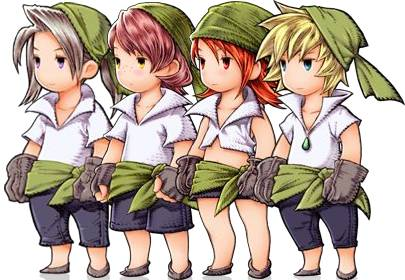
\includegraphics[width=\columnwidth]{./art/jobs/thief.jpg}\ofrow
	\accf{Thieves} are mobile melee fighters, who excel at "borrowing" items from enemies and have a heightened sense for worthwhile business. 
}
{Dagger}{Light Armor}{
	Level 1: & HP +20 & MP~+19 & AGI~+4 \\
	Level 2: & HP~+5  & MP~+10  & STR~+1 & DEF~+1 \\
	Level 3: & \multicolumn{3}{l}{Archetype Attribute Bonus} \\
	Level 4: & HP~+10 & MP~+5  & STR~+1 & DEF~+1 \\
	Level 5: & HP~+10 & MP~+10 & STR~+1 &        \\ 
	Level 6: & HP~+5  & MP~+5  & DEF~+2 & RES~+1 \\ 
	Level 7: & HP~+10 & MP~+10 & STR~+1 &        \\ 
	Level 8: & HP~+10 & MP~+5  & RES~+2 &        \\ 
	Level 9: & HP~+5  & MP~+10 & STR~+2 &        \\ 
	Level 10:& HP~+10 & MP~+10  & DEF~+1 
}{
	\ofjobtech{Steal}{3}{0r}{Single}{1u}{Make a DC 7 check and "borrow" something from the target if you succeed. Roll 1d and you get your Level times 20G on 1 or 2, a Potion on a 3, a Remedy on a 4, an Ether on a 5 and a Phoenix Down on a 6. The item may also be determined in any other way by the GM.}{}{1} \ofabilitygap
	\ofjobtech{Flee}{4}{0r}{3u}{Self}{You and all allies in the target area can move twice as fast when running away from enemies for 3 rounds.}{}{2} \ofabilitygap
	\ofjobtech{Poison Dart}{7}{0r}{Single}{4u}{The target makes a DC~8 check and suffers 1d damage and one of the following Status Effects of your choice for 3 rounds upon failure: Poison, Immobile, Sleep}{}{4}\ofabilitygap
	\ofjobtech{Vanish}{8}{0r}{Single}{Self}{You become invisible for up to  5 rounds or until you take an action. While invisible, you gain Blink and if you hit an Attack, you always score a Critical Hit.}{\blink}{6} \ofabilitygap
	\ofjobtech{Sticky Fingers}{6}{0r}{Single}{Self}{For the next 3 rounds, whenever you perform a successful Attack you can also use Steal on the same target without additional cost. Additionally, all items that you receive from Steal are doubled for this duration.}{}{8} \ofabilitygap
	\ofjobtech{Mirror Image}{25}{1r}{Single}{1u}{You create an exact copy of yourself that lasts for 3 rounds or until you create a new one. It acts with you on your turn, following your command. The clone can use the same abilities as you except this one.}{}{10}
}{
	\ofarchetypet{Ninja}
	{HP~+14 & MP~+11 & STR~+2}
	{\ofarchetypetecha{Throw}{4}{0r}{Single}{5u}{You throw a piece of equipment from your inventory on the target and deal an amount of damage depending on its equipment rank. The damage dealt is 1d for Beginner, 2d for Advanced and 3d for Expert level equipment. You can collect all thrown objects at the end of the battle.}{}}
	{\ofarchetypepassive{First Strike}{When an ally chooses you to take the next turn, you can immediately take it instead of waiting for a turn of the opposing party.}}
	{\ofarchetypereaction{Counter Attack}{When an enemy hits you with an Attack, you can immediately make an Attack on him if he is within range.}}
	{\ofarchetypetechb{Assassinate}{14}{0r}{Single}{3u}{Move to the target and make an Attack on him. If you hit, he makes a DC~7 check and suffers KO upon failure.}{\ko}}
}{
	\ofarchetypet{Treasure Hunter}
	{HP~+10 & MP~+20 & DEF~+1 & RES~+1}
	{\ofarchetypetecha{Quick Pockets}{6}{0r}{Single}{Self}{Make an Attack after which you can immediately use an Item.}{}}
	{\ofarchetypepassive{Gilionaire}{Whenever you deal damage to an enemy, you also receive an amount of Gil equal to the total damage dealt.}}
	{\ofarchetypereaction{Pickpocket}{Whenever you evade an Attack by an enemy, you can immediately use Steal on him without any cost.}}
	{\ofarchetypetechb{Gil Toss}{5}{0r}{Single}{5u}{Throw an amount of Gil on the target up to a maximum of 100G. The target suffers 1d damage for every 20G thrown. The money is destroyed in the process.}{}}
}
%
%
%
%
%
\ofjob{Tinker}
{
	\ofquote{"I don't give a rat's ass whether it's science or magical power. No, I guess if I had to choose, I'd rather put my money on the power of science."}{Cid}\\\\
	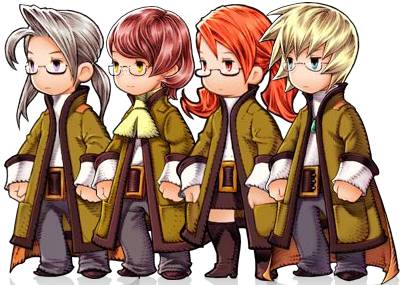
\includegraphics[width=\columnwidth]{./art/jobs/tinker2.jpg}\ofrow
	\accf{Tinkers} are technical experts who defeat their enemies by using the power of science. 
	They can create special items and devices that cause fantastic effects in combat. 
	Tinkers prove that any sufficiently advanced technology is indistinguishable from magic.	
}
{Bow or Gun or Spear}{Robe}{
	Level 1: & HP~+17 & MP~+24 & AGI~+2 & STR~+1 \\
	Level 2: & HP~+5  & MP~+10 & RES~+1 & DEF~+1 \\
	Level 3: & \multicolumn{3}{l}{Archetype Attribute Bonus}  \\
	Level 4: & HP~+5  & MP~+10 & STR~+1 & DEF~+1 \\
	Level 5: & HP~+10 & MP~+10  & STR~+1 \\
	Level 6: & HP~+10 & MP~+10 & RES~+1 \\
	Level 7: & HP~+5  & MP~+10 & STR~+1 & DEF~+1 \\
	Level 8: & HP~+10 & MP~+10 & RES~+1 \\
	Level 9: & HP~+10 & MP~+10 & RES~+1 \\
	Level 10:& HP~+5  & MP~+10 & RES~+2
}{
	\ofjobtech{Stimulant}{4}{0r}{Single}{1u}{The target gains Regen for 3 rounds.}{\regen}{1}\ofabilitygap
	\ofjobtech{Flamethrower}{4}{0r}{3u (front)}{Self}{Make an Attack against every enemy in the target area. When you hit, the damage dealt is of fire type.}{\fire}{2}\ofabilitygap
	\ofjobtech{Propel}{6}{0r}{1u}{Self}{You shoot up to 3u into the air from where you can move and act as usual. After 2 rounds, you land on the ground in your current position.}{}{4}\ofabilitygap
	\ofjobtech{Fortify Position}{10}{0r}{2u}{5u}{You create a special field in the target area for 3 rounds. All allies gain EnSTR and EnDEF as long as they are standing inside it.}{\enstr\enndef}{6}\ofabilitygap	
	\ofjobtech{Shockwave}{9}{0r}{3u}{Self}{Everyone in the target area except you receives 3d damage and is pushed back by 3u. In addition, all affected targets make a DC~8 check and suffer Immobile for 1 round upon failure.}{\immobile}{8}\ofabilitygap
	\ofjobtech{Pandora's Box}{26}{1r}{5u}{Self}{All enemies in the target area suffer 4d damage. In addition, all affected targets roll 1d and suffer the following Status Effects for 3 rounds based on the result: 1-Immobile, 2-Slow, 3-Silence, 4-Poison, 5-Blind, 6-Sleep.}{\immobile\slow\silence\poison\blind\sleep}{10}
}{
	\ofarchetypet{Chemist}
	{HP~+8 & MP~+17 & RES~+2}
	{\ofarchetypetecha{Turbo Vaccine}{6}{0r}{Single}{1u}{The target regains 1d HP and becomes Immune to Poison, Silence, Blind and flu-like viruses for 3 rounds.}{}}
	{\ofarchetypepassive{Item Lore}{You can use Items in a range of up to 3u and you may affect everyone within 1u of the target. Both effects also apply to the Stimulant, Turbo Vaccine and Mix Techs.}}
	{\ofarchetypereaction{Auto-Potion}{Whenever you suffer damage, you can immediately use an Item. You can only use this effect once per round.}}
	{\ofarchetypetechb{Mix}{10}{0r}{Single}{3u}{Use 2 Items on the target and then roll 1d. Targeted allies recover 3d HP on 1-2, gain Blink for 3r on 3-4 and Haste for 3r on 5-6. Targeted enemies suffer 3d damage on 1-2, Immobile for 3r on 3-4 and Slow for 3r on 5-6.}{\blink\haste\immobile\slow}}
}{
	\ofarchetypet{Machinist}
	{HP~+10 & MP~+10 & STR~+2 & DEF~+1}
	{\ofarchetypetecha{Autoturret}{8}{0r}{1u}{1u}{You create a turret in the target area for 3 rounds. At the start of each turn, deal damage equal to your current Level to one enemy within 3u of it.}{}}
	{\ofarchetypepassive{Synthesis}{You gain an additional STR+1, DEF+1 or RES+1 for every Materia that you have equipped.}}
	{\ofarchetypereaction{Ballistic Defense}{Whenever you would suffer damage from an enemy that is further than 2u away from you, make a DC 7 check. If you succeed, the damage dealt is halved.}}
	{\ofarchetypetechb{Satellite Beam}{12}{0r}{?}{?}{All affected enemies suffer 5d damage. Choose one of the following target shapes to determine the affected targets: draw a 1u thick ring around you with an outer radius of up to 8u \accf{or} draw a 1u wide line with both ends within 8u of you \accf{or} all enemies within 5u of you make a check and everyone who rolls an odd number is affected.}{}}
}
%
%
%
%
%
\ofjob{Time Mage}
{
	\ofquote{"Time... It will not wait."\\}{Ultimecia}\\\\
	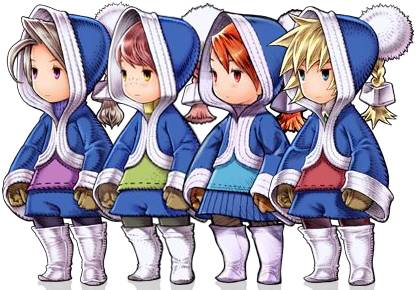
\includegraphics[width=\columnwidth]{./art/jobs/timemage.jpg}\ofrow
	\accf{Time Mages} are masters of time and space, who understand that imagination is more important than knowledge. 
	They manipulate the flow of time and bend the fabric of reality to their advantage.
}
{Staff}{Robe}{
	Level 1: & HP~+17 & MP~+27 & AGI~+2 & MAG~+1 \\
	Level 2: & HP~+5  & MP~+10 & RES~+1 & STR~+1 \\
	Level 3: & \multicolumn{3}{l}{Archetype Attribute Bonus}  \\
	Level 4: & HP~+10  & MP~+10 & MAG~+1 &        \\ 
	Level 5: & HP~+10 & MP~+10 & RES~+1 &		  \\ 
	Level 6: & HP~+5  & MP~+10 & DEF~+1 & RES~+1 \\ 
	Level 7: & HP~+5  & MP~+10 & RES~+2 \\ 
	Level 8: & HP~+10  & MP~+10 & DEF~+1 \\ 
	Level 9: & HP~+5  & MP~+10 & RES~+2 &        \\ 
	Level 10:& HP~+5  & MP~+10 & MAG~+1 &	RES~+1	  
}{
	\ofjobspell{Gravity}{6}{0r}{Single}{3u}{The target suffers 2d damage and can only move half his usual distance on his next turn.}{}{1}\ofabilitygap
	\ofjobspell{Haste}{8}{0r}{Single}{5u}{The target gains Haste for 3 rounds.}{\haste}{2}\ofabilitygap
	\ofjobspell{Slow}{8}{0r}{Single}{5u}{The target suffers Slow for 3 rounds.}{\slow}{2}\ofabilitygap
	\ofjobspell{Float}{8}{0r}{Single}{3u}{The target levitates up to 3u above the ground for 2 rounds. While allies can still move in the air, targeted enemies suffer Immobile for the duration.}{}{4}\ofabilitygap
	\ofjobspell{Graviga}{15}{1r}{2u}{6u}{All enemies in the target area suffer 6d damage and a Slow Field appears in the target area that lasts for 3 rounds.}{}{6}\ofabilitygap
	\ofjobspell{Stop}{16}{0r}{30u}{Self}{All enemies in the target area make a DC 8 check and suffer Sleep for 1 round upon failure.}{\sleep}{8}\ofabilitygap
	\ofjobspell{Banish}{26}{0r}{Single}{5u}{Temporarily banish the target into another dimension. If he is an ally, he can still take turns, but not interact with the battlefield. After 3 rounds, the target reappears in the same spot, anyone in the same space is pushed aside and suffers 6d damage. You cannot use Banish consecutively on the same target or if a previous cast is still active.}{}{10}
}{
	\ofarchetypet{Illusionist}
	{HP~+5 & MP~+20 & MAG~+2}
	{\ofarchetypespella{Warp}{6}{0r}{1u}{5u}{You teleport to an unoccupied location of your choice that you can see within 5u.}{}}
	{\ofarchetypepassive{Tunneling}{Whenever you cast a spell, you can choose to double its range and target distance by also doubling its MP cost.}}
	{\ofarchetypereaction{Quick Warp}{Whenever you are targeted by an Attack, you can attempt to Warp. In this case, you make the evasion check with advantage and if you succeed, the Warp spell takes effect in addition to the evasion. In either case, you have to respect the spell's MP cost.}}
	{\ofarchetypespellb{Exchange}{14}{0r}{Single}{10u}{Choose two targets within range and exchange their positions. Targeted enemies suffer an additional 4d damage. Targeted allies instead cause 4d damage to everyone within 2u of their new position. Also, both targets push aside anything that would obstruct their new spot.}{}}
}{
	\ofarchetypet{Oracle}
	{HP~+8 & MP~+17 & STR~+1 & RES~+1}
	{\ofarchetypespella{Extend}{5}{0r}{Single}{8u}{The duration of all Status Effects that the target is suffering or benefiting from, is extended by 3 rounds.}{}}
	{\ofarchetypepassive{Read Ahead}{Right before the start of each combat, you can take one extra turn, even if the enemy has a surprise round.}}
	{\ofarchetypereaction{Kismet}{When a spell or tech that targets someone within 5u takes effect, you can choose to delay it. In this case, the battle continues as usual and the ability instead takes effect on the target after 1 round. This effect does not stack.}}
	{\ofarchetypespellb{Quicken}{12}{0r}{Single}{5u}{The target takes an extra turn immediately before yours is finished. The round continues as usual afterwards, so you still have to pick the next combatant for your side. You can only use this ability once per round.}{}}
}
%
%
%
%
%
\ofjob{Warrior}
{
	\ofquote{"I dreamt I was a moron."\\}{Squall}\\\\
	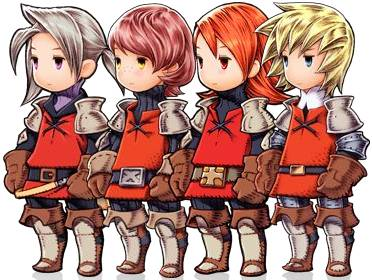
\includegraphics[width=\columnwidth]{./art/jobs/warrior.jpg}\ofrow
	\accf{Warriors} are specialists in melee combat, because of their strong physical offense and defense. 
	They are proficient with powerful swords and armor, allowing them to become even more dangerous and durable. 
}
{Sword}{Light or Heavy Armor}{
	Level 1: & HP +25 & MP~+18 & AGI~+3 & STR +1 \\
	Level 2: & HP~+10 & MP~+5  & STR~+1 & DEF~+1 \\
	Level 3: & \multicolumn{3}{l}{Archetype Attribute Bonus}  \\
	Level 4: & HP~+10 & MP~+5  & STR~+2 &        \\ 
	Level 5: & HP~+10  & MP~+10 & DEF~+1 \\ 
	Level 6: & HP~+10 & MP~+5  & DEF~+1 & RES~+1 \\ 
	Level 7: & HP~+10 & MP~+10  & STR~+1 &        \\ 
	Level 8: & HP~+10 & MP~+5  & RES~+2 &        \\ 
	Level 9: & HP~+5  & MP~+10 & STR~+1 & DEF~+1 \\ 
	Level 10:& HP~+10 & MP~+5  & DEF~+2 &         
}{
	\ofjobtech{Rush}{3}{0r}{Single}{1u}{Make an Attack against the target. If you hit, you push him back by 1u on top of the damage dealt.}{}{1}\ofabilitygap
	\ofjobtech{Beatdown}{6}{0r}{Single}{1u}{Make an Attack where the target has Advantage on the evasion check. If you hit, you score a Critical Hit.}{}{2}\ofabilitygap
	\ofjobtech{Vitality}{5}{0r}{Single}{Self}{For the next 3 rounds, when an effect restores your HP or MP, the amount is doubled. Also, when you have to make a check to resist a negative effect, its DC is reduced by 2.}{}{4}\ofabilitygap
	\ofjobtech{Army of One}{10}{0r}{3u}{Self}{Make an Attack against every enemy in the target area by making one damage roll that applies to all affected targets that fail to evade. After using the ability, you can move next to any of the affected targets.}{}{6}\ofabilitygap
	\ofjobtech{Bravery}{10}{0r}{2u}{Self}{You and all allies within the target area gain EnSTR and EnMAG for 2 rounds.}{\enstr \enmag}{8}\ofabilitygap
	\ofjobtech{Omnislash}{28}{0r}{Single}{1u}{Make 3 separate Attacks against the target. Each time he rolls 4 or less on an evasion check, you score a Critical Hit.}{}{10}
}{
	\ofarchetypet{Dark Knight}
	{HP~+5 & MP~+15 & DEF~+1 & RES~+2}
	{\ofarchetypetecha{Defensebreak}{6}{0r}{Single}{1u}{Make an Attack on the target. If you hit, he suffers DeDEF and DeRES for 2 rounds on top of the damage dealt.}{\dedef \deres}}
	{\ofarchetypepassive{Souleater}{Whenever you successfully Attack an enemy, you can additionally inflict dark damage equal to half of the total damage dealt, to yourself and all enemies within~3u.}}
	{\ofarchetypereaction{Blood Price}{Whenever an enemy that you can see spends MP, you can force him to spend an equal amount of HP instead if he has enough HP to do so. Afterwards, increase your own HP by half the amount spent.}}
	{\ofarchetypetechb{Berserk}{10}{0r}{Single}{5u}{For the next 3 rounds the target can only take the Attack action, but every successful Attack is a Critical Hit. If you target an enemy with this ability, he makes a DC~8 check and only suffers this effect upon failure.}{}}
}{
	\ofarchetypet{Samurai}
	{HP~+16 & MP~+9 & STR~+2}
	{\ofarchetypetecha{Focus}{5}{0r}{Target}{Self}{For the next 3 rounds, whenever you Attack an enemy, he has Disadvantage on the the evasion check.}{}}
	{\ofarchetypepassive{Cripple}{Whenever the target of your Attacks rolls a 5 or less on the evasion check he additionally suffers one of the following Status Effects of your choice for 1 round upon failure: Immobile, Blind, DeSTR.}}
	{\ofarchetypereaction{Bushido}{You can evade Techs by passing an evasion check the same way that you evade Attacks. Also, whenever you evade an Attack or Tech, you regain an amount of MP equal to your current Level.}}
	{\ofarchetypetechb{Razor Gale}{8}{0r}{5u (line)}{Self}{Everyone in the target area suffers 4d wind damage.}{\wind}}
}
%
%
%
%
%
\ofjob{White Mage}
{
	\ofquote{"Hey, that’s Cloud’s line! ’It’s too dangerous, I can’t get you involved...' Blah blah blah."\\}{Aerith}\\\\
	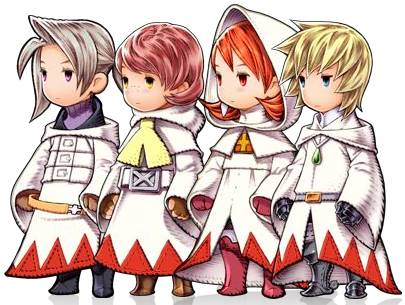
\includegraphics[width=\columnwidth]{./art/jobs/whitemage.jpg}\ofrow
	\accf{White Mages} are experts of defensive magic and boast a variety of recovery and protective spells.
	While mediocre in physical combat, they also feature incredible resistance against magic. 
}
{Staff}{Robe}{
	Level 1: & HP~+19 & MP~+25 & AGI~+2 & STR~+1 \\
	Level 2: & HP~+5  & MP~+10 & MAG~+1 & RES~+1 \\
	Level 3: & \multicolumn{3}{l}{Archetype Attribute Bonus} \\
	Level 4: & HP~+10 & MP~+5 & MAG~+1 & DEF~+1	  \\
	Level 5: & HP~+5  & MP~+10 & RES~+1 &	STR~+1  \\ 
	Level 6: & HP~+5  & MP~+5 & MAG~+2 &        \\ 
	Level 7: & HP~+10  & MP~+10 & RES~+1 & DEF~+1 \\ 
	Level 8: & HP~+5 & MP~+5  & MAG~+2 & DEF~+1 \\ 
	Level 9: & HP~+5  & MP~+10 & RES~+1 &	MAG~+1   \\ 
	Level 10:& HP~+10 & MP~+10 & RES~+1 &	        
}{	
	\ofjobspell{Cure}{4}{0r}{Single}{3u}{The target regains 2d HP.}{}{1}\ofabilitygap
	\ofjobspell{Drain}{6}{0r}{Single}{3u}{Deal 1d damage to the target and increase your own HP by the total amount of damage dealt.}{}{2}\ofabilitygap
	\ofjobspell{Esuna}{6}{0r}{Single}{5u}{You remove all negative Status Effects except KO from the target.}{}{4}\ofabilitygap
	\ofjobspell{Curaga}{14}{1r}{2u}{5u}{Everyone in the target area regains 6d HP.}{}{6}\ofabilitygap
	\ofjobspell{Clear}{6}{0r}{5u}{50u}{You remove one active Field Effect within range.}{}{6}\ofabilitygap
	\ofjobspell{Holy}{21}{2r}{Single}{12u}{You deal 6d+45 holy damage to the target.}{\holy}{8}\ofabilitygap
	\ofjobspell{Auto-Life}{28}{2r}{Single}{3u}{You summon a guardian angel that watches over the target. The next time he falls KO, he is instantly revived with 1 HP. This effect does not stack and if not activated, it expires when the target goes to sleep.}{\ko}{10}
}{
	\ofarchetypet{Sage}
	{HP~+11 & MP~+9 & MAG~+2 & STR~+1}
	{\ofarchetypespella{Sleep}{6}{0r}{Single}{5u}{The target makes a DC 8 check and suffers Sleep for 3 rounds upon failure.}{\sleep}
		\vspace*{0.1cm}\\ \ofarchetypespella{Silence}{6}{0r}{Single}{5u}{The target makes a DC 8 check and suffers Silence for 3 rounds upon failure.}{\silence}}
	{\ofarchetypepassive{Ancient Wisdom}{When you inflict one or more Status Effects on a target, you can also inflict DeDEF or DeRES on him for 3 rounds.}}
	{\ofarchetypereaction{Absorb MP}{When you are the target of an enemy ability, increase your MP by half the amount that the caster spent on it.}}
	{\ofarchetypespellb{Curse}{14}{1r}{Single}{5u}{The target makes a DC~9 check and upon failure he suffers 4d damage as well as Poison and Zombie for 3 rounds.}{}}
}{
	\ofarchetypet{Medic}
	{HP~+7 & MP~+13 & RES~+2 & DEF~+1}
	{\ofarchetypespella{Protect}{4}{0r}{Single}{5u}{The target gains EnDEF for 3 rounds.}{\enndef} \vspace*{0.1cm}\\ \ofarchetypespella{Shell}{4}{0r}{Single}{5u}{The target gains EnRES for 3 rounds.}{\enres}}
	{\ofarchetypepassive{Doctor's Code}{Whenever you use Magic on an ally within 1u, you can immediately use an Item on him in addition.}}
	{\ofarchetypereaction{No Collateral}{Whenever you would be affected by a spell or tech that you are not the primary target of, you can choose that you and all other secondary targets are unaffected.}}
	{\ofarchetypespellb{Full-Life}{22}{2r}{Single}{5u}{You remove the KO status from the target and fully restore his HP.}{\ko}}
}
\ofsubsection{Equipment}
%
\ofquote{"Oh, really, don't you know? These days all it takes for your dreams to come true is money and power."\\}{President Shinra}\\
%

\includegraphics[width=\columnwidth]{./art/images/ff1.jpg}
%
\vfill
%
A character's combat potency can be further improved through \accf{Equipment}. 
While \accf{Weapons} increase the damage dealt, \accf{Armor} protects against incoming damage and \accf{Accessories} are miscellaneous pieces that complement a character's gear.
In addition, all equipment pieces may provide boosts to attributes or other useful effects. 
Every character can wear one weapon, one armor and two accessories. 
All weapons have a range of 1u unless specified otherwise. 
Instead of armor, characters can also wear regular clothes which only provide DEF~+1.
Accessories can be worn by everyone, but characters can only equip specific weapon and armor types depending on their job.
Equipment pieces are classified into different \accf{Equipment Classes} depending on their potency and rarity.
While everyone can carry Beginner equipment, characters need to be at least Level 4 to use Advanced equipment and Level 8 to use Expert equipment. 
All characters can also use \accf{Items}, that provide quick benefits in and outside of combat, but are consumed after a single use.
%
\vfill
%
All items and unequipped possessions are stored in your character's \accf{Inventory}.
Equipment and items can be looted from defeated foes and treasure chests or earned as rewards for completing a given task. 
But the party may also buy or sell specific goods to shops and merchants. 
The currency used for trading is called \accf{Gil} and typically comes in the form of golden coins.
You can try buying and selling almost anything, as long as someone is willing to trade.
%
\vfill
%
\ofboxwithtitle{Example: Trading}{
	Terra and her party visit an auction house to bet on rare items.
	Today is their lucky day, the item up for bid is a talking Chocobo! 
	The party is impressed by this talented creature and decides to bid all of their savings, a total of 10000 Gil!
	It looks like they are outbidding everyone, but in the last second a loving father bids 500000 Gil and acquires the Chocobo as a present for his son.
	Maybe the party has better luck (or more money) next time...
}
%
\newpage
%
\ofquote{"Cloud, sign this. It's a contract that says when the war is over, all the materia will belong to me."}{Yuffie}\\\\
%
Weapons and armor can be improved through the use of \accf{Materia}.
Materia usually appear as crystal-like artifacts that concentrate magical forces inside them, ready to be used by anyone.
They can be slotted into weapons and armor to grant their wielder additional abilities or effects.
Slotted Materia can also be removed and swapped out easily. 
Although their availability may vary, Materia can be stored and traded just as any other item.
Unless explicitly stated otherwise, every weapon or armor can carry one Materia, but clothes and accessories cannot carry any Materia.
Materia can be divided into two categories: command and support Materia.
Command materia allow the wielder of the imbued equipment to use new abilities, while support Materia grant passive effects.
If a Materia allows the use of an existing ability, the user has to adhere to its usual rules including MP cost and cast time.
Finally, some Materia can only be slotted into weapons, while others are only compatible with armor.
%
\vfill
%
\ofquote{"Yes, the twelve legendary weapons. They are weapons. They are legendary. There are even twelve of them."}{Ghido}\\\\
%
Unless the GM decides otherwise, every character gains 1500 Gil at Level~1, from which they can buy their starting equipment as follows:
\ofrow
\ofbullet{Buy any Beginner weapon for 500 Gil or a Beginner Myhtril weapon for 250 Gil.}
\ofbullet{Buy any Beginner armor for 500 Gil, a Beginner Myhtril armor for 250 Gil, or clothes for 100 Gil.}
\ofbullet{Optionally, you can buy one Beginner accessory for 500 Gil.}
\ofbullet{Optionally, you can buy any set of Items that you can afford.}
\ofbullet{Optionally, you can buy one Materia that you can afford.}
The following pages give various examples of Items, Materia and Equipment pieces that you can choose.
The equipment classes of the listed weapons and armor are decided by the GM.
Make sure to read the \accf{Notes}, which define special rules and effects for different equipment categories.
Finally, the table below summarizes the most important points about Equipment Classes.
%
\vfill
%
\oftable{p{0.125\columnwidth} p{0.225\columnwidth} p{0.15\columnwidth} p{0.15\columnwidth} p{0.3\columnwidth}}
{\accf{Level} & \accf{Equipment Class} & \accf{Weapon DMG} & \accf{Armor\newline DEF/RES} & \accf{Value}}
{
 	\\
	1 - 3  & Beginner 		& 1d & +0 / +0   & \textasciitilde 500 Gil\\\\
	4 - 7  & Advanced   & 2d & +1 / +1   & \textasciitilde 2000 Gil\\\\
	8 - 10 & Expert	 		& 3d & +2 / +2   & >4000 Gil 
}
%
\clearpage
%
\newcommand{\ofequipnote}[1]{\multicolumn{2}{p{\columnwidth}}{\hspace*{-0.15cm}\parbox{0.97\columnwidth}{#1}}}
\oftable{p{0.22\columnwidth} p{0.7\columnwidth}}
{\accf{Bow} & \accf{Effect}}
{
	Mythril~Bow & Has an additional Materia slot. \ofrow
	Elfin Bow & Whenever you Attack a target that is suffering a Status Effect, add 3 to the damage dealt. \ofrow 
	Killer Bow & On a Critical Hit, the target instantly suffers KO. \ofrow
	Crossbow & This weapon does not suffer from the same penalty as other bows, so you can move and Attack on the same turn. But its range is only 3u. \ofrow
	Aplu & Attacks by this weapon ignore all effects that would grant the target advantage on the evasion check. \ofrow
%	Selene & When the target of your Attack rolls a 5 or less on the evasion check, he suffers Sleep for 3 rounds.\ofrow
	Anteros & When the target of your Attack rolls a 5 or less on the evasion check, he suffers Blind for 3 rounds.\ofrow
	\ofequipnote{\accf{Note:} Bows have 5u range. If you Attack with a bow or use a Tech with an Attack and you move on the same turn, the target has Advantage on the evasion check.\phantom{y}}
}
%
\vfill
%
\oftable{p{0.22\columnwidth} p{0.7\columnwidth}}
{\accf{Gun} & \accf{Effect}}
{
	Mythril~Gun & Has an additional Materia slot. \ofrow
	Fomalhaut & The damage dealt by this weapon is of magical type. \ofrow
	Tiny Bee & On Critical Hit, you gain 10 Limit Points.\ofrow  
	Machine Gun & If the target evades your Attack, he still suffers 1d damage. \ofrow
	Dragon Breath & Damage dealt by this weapon is of fire type. Also, everyone who ends his turn within 1u of you, suffers 3 fire damage.\ofrow
	Spirit \newline Cannon & Whenever you successfully Attack a target who is suffering the Zombie status, you score a Critical Hit.\ofrow
	\ofequipnote{\accf{Note:} Guns have 3u range. Unlike Bows, their damage is not directly increased by STR. Instead, a gun's DMG is increased by 1d for every 3 STR that its wielder has.}
}
%
\vfill
%
\oftable{p{0.22\columnwidth} p{0.7\columnwidth}}
{\accf{Spear} & \accf{Effect}}
{
	Mythril~Spear & Has an additional Materia slot. \ofrow
	Gae Bolg & Score a Critical Hit also when your opponent rolls a 3 on the evasion check. \ofrow
	Vel & The damage dealt by all of your Techs is of magical type. \ofrow
	Longinus & When the target of your Attack rolls a 5 or less on the evasion check, he suffers Sleep for 3 rounds. \ofrow 
	Trident & Attacks target both the original target and anyone directly behind him. \ofrow
	Naginata & On every Critical Hit, triple your usual damage, instead of just doubling it.\ofrow
	\ofequipnote{\accf{Note:} Spears have 2u range.}
}
%
\newpage
%
\oftable{p{0.22\columnwidth} p{0.7\columnwidth}}
{\accf{Dagger} & \accf{Effect}}
{	
	Mythril Knife & Has an additional Materia slot.\ofrow
	Nightshade & When the target of your Attack rolls a 5 or less on the evasion check, he suffers Poison for 3 rounds.\ofrow
	Assassin Knife & On a Critical Hit, the target instantly suffers KO. \ofrow
	Orichalcum & When you use a Fortune Die on an Attack damage roll, add 2 to the total amount. \ofrow
	Gladius  & The DC of all checks related to stealing is reduced by 1.\ofrow
	Main Gauche & DEF~+1. Grants another DEF~+1 if equipped as second Dagger.\ofrow
	Subtle Smile & If there is an ally of you within 1u of the target, add 3 to the damage dealt by Attacks with this weapon.\ofrow
	\ofequipnote{\accf{Note:} You can equip a second Dagger when you are not wearing any Accessories. In this case, you can make a second Attack with the other weapon instead of your usual movement.\phantom{y}}
}
%
\vfill
%
\oftable{p{0.22\columnwidth} p{0.7\columnwidth}}
{\accf{Sword} & \accf{Effect}}
{
	Mythril Sword & Has an additional Materia slot. \ofrow
	Buster Sword & When the target of your Attack rolls a 5 or less on the evasion check, the damage dealt ignores his DEF. \ofrow
	Gunblade & You can make an up to 3u long ranged Attack. In this case, you do not add your STR to the damage dealt.\ofrow
	Organyx & Whenever you successfully Attack an enemy, you regain 2 MP. \ofrow
	Bloodsword & When you reduce an enemy to 0 HP, you regain an amount of HP equal to your current Level. \ofrow
	Murasame & The range of all your Techs is increased by 1u. \ofrow
	Yoshihara & Whenever you perform a counter Attack through an evasion check, you always score a Critical Hit.\ofrow
	Vorpal Blade & On Critical Hit, quadruple your usual damage, instead of just doubling it. \ofrow
	Save the \newline Queen & Whenever you or an ally within 1u is affected by Magic, you can halve the damage suffered by passing a DC 9 check.\ofrow
	\ofequipnote{\accf{Note:} When rolling an evasion check, you can make a counter Attack not only when you roll a 12 but also when you roll an 11.}
}
%
\clearpage
%
\oftable{p{0.22\columnwidth} p{0.7\columnwidth}}
{\accf{Staff} & \accf{Effect}}
{
	Mythril Staff & Has an additional Materia slot. \ofrow
	Healing Staff & Whenever you restore HP with Magic, add 2 to the amount. \ofrow 
	Oak Staff & While you are concentrating, you can use the Defend action. \ofrow
	Malboro Staff & When you use Magic that requires the target to pass a check, its DC is increased by 1.\ofrow
	Rune Staff & When you deal magical damage to an enemy that is suffering a Status Effect, he also suffers Silence for 3 rounds. \ofrow
	Power Staff & Whenever you perform a successful Attack, also add your MAG to the damage dealt. \ofrow
	Sage's Staff & You can add the holy type to damage dealt by Attacks and Magic.\ofrow
	Oracle Bone & The range of all HP restoring or Status Effect causing spells is increased by 1u.\ofrow
	\ofequipnote{\accf{Note:} Staves increase the wielder's maximum MP by 5 per increase in equipment class (for example a Beginner staff grants maximum MP~+5). In exchange, staves cannot have more than 1d damage.}
}
%
\vfill
%
\oftable{p{0.22\columnwidth} p{0.7\columnwidth}}
{\accf{Rod} & \accf{Effect}}
{
	Mythril Rod & Has an additional Materia slot. \ofrow
	Elemental Rod & This weapon has to be of a specific element (e.g. fire) and can have an according name (e.g. Flame Rod). Whenever you deal damage of that element, add 2 to the amount.\ofrow
	Adamantine Rod & This weapon does not suffer from the same penalty as other rods. It has the same DMG as any other weapon in the same class.\ofrow
	Stardust Rod & When you reduce an enemy to 0 HP, you regain an amount of MP equal to your current Level. \ofrow
	Lilith Rod & While you are concentrating, you can still use the Dash action. \ofrow
	Whale Whisker & You can add the water type to damage dealt by Attacks and Magic.\ofrow
	Magus Rod & When you use a Fortune Die on a roll related to your Magic, add 2 to the total amount. \ofrow
	\ofequipnote{\accf{Note:} Rods increase the wielder's MAG by one per increase in equipment class (for example a Beginner rod grants MAG~+1). In exchange, rods cannot have more than 1d damage.}
}
%
%
\newpage
%
\oftable{p{0.3\columnwidth} p{0.62\columnwidth}}
{\accf{Heavy Armor} & \accf{Effect}}
{
	Mythril Armor & Has an additional Materia slot.  \ofrow
	Crystal Mail & Resilience: ice  \ofrow
	Demon Mail & Resilience: dark  \ofrow
	Diamond Armor & Resilience: lightning  \ofrow
	Dragon Mail & Resilience: fire \ofrow
	Knight's Armor & STR +1 \ofrow
	Mirror Mail & Immunity: Silence \ofrow
	Achilles & DEF +1 \ofrow
	Fullplate & Maximum HP +5 \ofrow
	Karuta-gane & When you Dash you can move twice as far as usual. \ofrow
	\ofequipnote{\accf{Note:} All Heavy Armor provide an additional DEF +2.}
}
%
\vfill
%
\oftable{p{0.3\columnwidth} p{0.62\columnwidth}}
{\accf{Light Armor} & \accf{Effect}}
{
	Mythril Vest & Has an additional Materia slot. \ofrow
	Gaia Gear & Resilience: earth \ofrow
	Kenpo Gi & Immunity: Blind \ofrow
	Minerva & Resilience: ice \ofrow
	Mirage Vest & Immunity: Sleep \ofrow 
	Ninja Gear & Immunity: Immobile \ofrow			 
	Power Vest & STR +1 \ofrow
	Red Jacket & Resilience: fire\ofrow
	Survival Vest & Maximum HP +5 \ofrow
	Flak Jacket & Resilience gainst damage dealt by Bows and Guns. \ofrow
	Nemean \newline Lionskin & Resilience gainst damage dealt by Swords and Daggers. \ofrow
	Behemoth Suit & RES +1 \ofrow
	\ofequipnote{\accf{Note:} All Light Armor provide an additional DEF +1 and RES +1.\phantom{y}}
}
%
\vfill
%
\oftable{p{0.3\columnwidth} p{0.62\columnwidth}}
{\accf{Robe} & \accf{Effect}}
{
	Silk Robe &  Has an additional Materia slot. \ofrow
	Black Robe & Immunity: Poison \ofrow
	Coat of \newline Many Colors & DEF +1\newline \ofrow
	Cotton Robe & Resilience: wind \ofrow
	Luminous Robe & Resilience: holy \ofrow
	Magus Robe & MAG +1 \ofrow
	Scholar's Robe  & Maximum MP +5  \ofrow
	Necromancer Shroud & Resilience: dark\newline \ofrow
	White Robe & Immunity: Sleep \ofrow
	Hagoromo & Immunity to all Field effects. \ofrow
	\ofequipnote{\accf{Note:} All Robes provide an additional RES +2.}	
}
%
\clearpage
%
\oftablewide{p{0.32\columnwidth} p{0.25\columnwidth} p{1.45\columnwidth}}
{\accf{Accessory} & \accf{Class} & \accf{Effect}}
{
	 Mythril Shield & Beginner & DEF +1  \ofrow
	 Power Armlet & Beginner & STR +1 \ofrow
	 Rune Bracers & Beginner & RES +1 \ofrow
	 Crystal Ring & Beginner & MAG +1 \ofrow
	 Battle Boots & Beginner & Immunity: Immobile  \ofrow
	 Silver Glasses & Beginner & Immunity: Blind  \ofrow
	 Star Pendant & Beginner & Immunity: Poison  \ofrow
	 White Cape & Beginner & Immunity: Silence  \ofrow
	 Berserker Badge & Beginner & You gain EnSTR as long as your current MP is 5 or less. \ofrow
	 Force Ring & Beginner & You gain EnMAG as long as your MP is at its maximum.\ofrow
	 Ninja Tabi & Beginner & Whenever you use the Dash action, you can move twice as far as usual.\ofrow
	 Life Pendant & Beginner & Whenever you recover from KO, you gain Regen for 3 rounds. \ofrow
	 Utility Belt & Beginner & You can use the Re-Equip action and still take another action.\ofrow
	 Buckler & Beginner & Whenever you use the Defend action in combat, you also regain 3 HP.\ofrow
	 Silent Boots & Advanced & Your footsteps are completely silent. \ofrow
	 Thief Gloves & Advanced & You have Advantage on all checks related to stealing. \ofrow
	 Protect Ring & Advanced & Whenever you suffer an Attack, you gain EnDEF for 1 round.\ofrow
	 Elemental \newline Cufflink & Advanced & This Accessory is of one elemental type (e.g. Fire Cufflink). Whenever you deal damage of that type, add 2 to the damage dealt. \ofrow
	 Item Holder & Advanced & While not in combat, you can put one Item into it. During combat, you can use this Item and still take another action.\ofrow
	 Circlet & Advanced & RES +1, MAG +1\ofrow
	 Grand Helmet & Advanced & STR +1, DEF +1\ofrow
	 Safety Bit & Advanced & RES~+1, Immunity: KO \ofrow 
	 Champion Belt & Advanced & STR +1, Immunity: DeATR \ofrow
	 Germinas Boots & Advanced & You can jump twice as high as usual.  \ofrow
	 Black Belt & Advanced & Maximum HP +10  \ofrow
     Heart Ring & Advanced & Maximum MP +10  \ofrow
	 Moogle Charm & Advanced & Glows when there is a monster within 50u of you.  \ofrow
	 Muscle Belt & Advanced & Whenever the target of your Attacks rolls 3 or less on the evasion check, you score a Critical Hit. \ofrow
 	 Aegis Shield & Expert & Whenever you are targeted by Magic that does not involve a check already, you can try to pass a DC~10 check to avoid its effect.\ofrow
	 Rosetta Stone & Expert & You are able to understand any written or spoken language. \ofrow
	 Hermes Shoes & Expert & In every battle, you have Haste on your first turn. Immunity: Slow \ofrow
	 Hero's Shield & Expert & DEF +1, RES +1, Immunity: Sleep \ofrow
	 Protect Bangle & Expert & You gain EnDEF and EnRES as long as your HP is below 50\% of its maximum. \ofrow
	 Feather Boots & Expert & You can levitate up to 1u above the ground. \ofrow
	 Hermes Sandals & Expert & AGI~+1 \ofrow
	 Divine Sandals & Expert & You can walk on water and other liquids. \ofrow
	 Genji Helmet & Expert & RES~+2, DEF~+1.\ofrow
	 Genji Shield & Expert & DEF~+2, RES~+1.\ofrow
	 Genji Gloves & Expert & STR~+2, MAG~+2.\ofrow
	 Gold Hairpin & Expert & The MP costs of all your abilities are reduced by 2.  \ofrow
 	 Ribbon & Expert & In all checks to resist a Status Effect, the DC is reduced by 2. \ofrow
	 \multicolumn{3}{p{2\columnwidth}}{\hspace*{-0.15cm}\accf{Note:} For some accessories it does not make sense to wear two of the same kind (for example shields).}
}
%
\clearpage
%
\oftablewide{p{0.3\columnwidth} p{0.18\columnwidth} p{1.5\columnwidth}}
{\accf{Item} & \accf{Value} & \accf{Effect}}
{
	Gysahl Greens & 25 Gil & Vegetable well-known as a Chocobo's favorite food. \ofrow
	Antidote & 50 Gil & Removes Poison. \ofrow
	Eyedrops & 50 Gil & Removes Blind.  \ofrow 
	Echo Grass & 50 Gil & Removes Silence.  \ofrow 
	Gold Needle & 50 Gil & Remove Immobile. \ofrow
	Arctic Wind & 100 Gil & The target suffers 2d ice damage. \ofrow
	Bomb Fragment & 100 Gil & The target suffers 2d fire damage. \ofrow
	Lightning Gem & 100 Gil & The target suffers 2d lightning damage. \ofrow
	Potion & 100 Gil & The target regains 8 HP. \ofrow
	Holy Water & 150 Gil & Removes Zombie.\ofrow
	Ether & 150 Gil & The target regains 12 MP. \ofrow
	Light Curtain & 200 Gil & The target gains EnDEF for 3 rounds.\ofrow
	Lunar Curtain & 200 Gil & The target gains EnRES for 3 rounds. \ofrow
	Giant's Tonic & 200 Gil & The target gains EnSTR for 3 rounds.\ofrow
	Faerie's Tonic & 200 Gil & The target gains EnMAG for 3 rounds.\ofrow
	Elemental Oil & 250 Gil &  This Item is of one elemental type (e.g Fire Oil). Apply it to your weapon and your next Attack deals an additional 6 damage of that element type. \ofrow
	Malboro Vine & 250 Gil & The target makes a DC 8 check and suffers Poison for 3 rounds upon failure.\ofrow
	Remedy & 250 Gil & Removes all negative status effects, except KO.\ofrow
	Sleep Powder & 250 Gil & The target makes a DC 8 check and suffers Sleep for 3 rounds upon failure.\ofrow
	Scanner & 300 Gil & Analyses the target thoroughly and know his Resiliences, Weaknesses, Immunities, as well as his current HP and MP.\ofrow
%	Hero Drink & 300 Gil & The target gains EnSTR and EnMAG for 3 rounds.\ofrow
	Warp Stone & 300 Gil & You teleport to a place you can see within 10u.\ofrow
	Spider Web & 350 Gil & The target makes a DC 8 check and suffers Slow for 3 rounds upon failure.\ofrow
	Hi-Potion & 400 Gil & The target regains 20 HP. \ofrow
	Turbo Ether & 500 Gil & The target regains 30 MP. \ofrow
	Vaccine & 500 Gil & Removes Poison and the target becomes Immune to it for the rest of the battle.\ofrow
	Megaphone & 500 Gil & Removes Silence and the target becomes Immune to it for the rest of the battle.\ofrow
	Magic Lenses & 500 Gil & Removes Blind and the target becomes Immune to it for the rest of the battle.\ofrow
	Pain Killer & 500 Gil & Removes Immobile and the target becomes Immune to it for the rest of the battle.\ofrow
	Phoenix Down & 500 Gil & Removes KO and the target regains 1 HP.\ofrow
	Dark Matter & 500 Gil & The target suffers 6d dark damage \ofrow
	X-Potion & 650 Gil & The target fully regains all HP.\ofrow
	Transfusion & 800 Gil & Removes Zombie and the target becomes Immune to it for the rest of the battle. \ofrow 
	Silver Hourglass & 800 Gil & Removes Slow and the target gains Haste for 3 rounds.\ofrow
	Mega-Potion & 800 Gil & Everyone within 1u regains 6d HP.  \ofrow
	X-Ether & 900 Gil & The target fully regains all MP.\ofrow
	Elixir & 1000 Gil & The targets fully regains HP and MP. \ofrow
	Tent & 1000 Gil & Allows the party to sleep outside comfortably. \ofrow
	Magicite Shard & 1000 Gil & Roll 1d, based on the result use the following summoning abilities: \newline 1-Ifrit, 2-Shiva, 3-Ramuh, 4-Odin, 5-Phoenix, 6-Bahamut.\ofrow
	Gold Hourglass & 1000 Gil & Time freezes for everyone except yourself within 5u for 10 seconds (1 round). \ofrow
	Summon Magicite & 1500 Gil & This Item is for one Summon (e.g. Ifrit Magicite). When used it activates the summoning ability of that Summon. \ofrow
	Mega-Elixir & 1500 Gil & Everyone within 1u fully regains their HP and MP.\ofrow
	Mega-Phoenix & 2000 Gil & Removes KO from everyone within 3u and fully restores their HP and MP.	
}
%
\clearpage
%
\oftablewide{p{0.36\columnwidth} p{0.16\columnwidth} p{1.45\columnwidth}}
{\accf{Command Materia} & \accf{Value} & \accf{Effect}}
{
	Fire Materia & 500 Gil & Allows you to use the "Fire" ability (see Black Mage job) \ofrow
	Ice Materia & 500 Gil & Allows you to use the "Blizzard" ability (see Black Mage job) \ofrow
	Bolt Materia & 500 Gil & Allows you to use the "Thunder" ability (see Black Mage job) \ofrow  
	Medic Materia & 500 Gil & Allows you to use the "First Aid" ability (see Sentinel job) \ofrow   
	Rage Materia & 500 Gil & Allows you to use the "Beatdown" ability (see Warrior job)\ofrow   
	Courage Materia & 500 Gil & Allows you to use the "Flee" ability (see Thief job) \ofrow    
	Kung-Fu Materia & 500 Gil & Allows you to use the "Kick" ability (see Monk job) \ofrow 
	Impromptu Materia & 750 Gil & Allows you to use the "Improvise" ability (see Bard job) \ofrow
	Mirage Materia & 750 Gil & Allows you to use the "Image" ability (see Summoner job) \ofrow
	Reflect Materia & 750 Gil & Whenever you are targeted by Magic, you immediately reflect its effect back to its caster. This item is destroyed after its effect is used. (armor only)\ofrow
	Decoy Materia & 750 Gil & Whenever you fail to evade an Attack, you can immediately summon a decoy that absorbs all the damage dealt. This item is destroyed after its effect is used. (armor only)\ofrow 
	Restore Materia & 750 Gil & Allows you to use the "Cure" ability (see White Mage job) \ofrow
	Dragon Materia & 750 Gil & Allows you to use the "Fire Breath" ability (see Dragoon job) \ofrow
	Runic Materia & 1000 Gil & Whenever you are targeted by Magic, you can negate its effect and increase your MP by the same amount that its caster spent on the action. This item is destroyed after its effect is used. (armor only) \ofrow 
	Signal Materia & 1250 Gil & You can use your action to shoot an orb of light into the air that is visible from up to 1000u. (weapon only) \ofrow 
	Bomb Materia & 1250 Gil & You can use your action to create a blast wave that pushes everyone within 1u of you back by up to 2u. \ofrow 
	Vacuum Materia & 1250 Gil & You can use your action to pull all enemies within 3u towards you by up to 2u. (armor only) \ofrow
	Fly Materia & 1500 Gil & Allows you to use the "Propel" ability (see Tinker job) \ofrow
	Time Materia & 1500 Gil & Allows you to use the "Haste" ability (see Time Mage job)\ofrow   
	Item Materia & 1500 Gil & Allows you to use the "Quick Pockets" ability (see Thief job) \ofrow   
	Jump Materia & 1500 Gil & You can use your action to make a 5u high or long jump. \ofrow
	Magnifying Materia & 1500 Gil & You can conjure a magnifying lens that allows to see everything in a location up to 5000u away as if it was right next to you (weapon only). \ofrow
	Mend Materia & 2000 Gil & You can use your action to remove one Status Effect that your are suffering. \ofrow
	Wet Floor Materia & 2000 Gil & You can use your action to create a Slippery Field that is centered around a point within 3u, reaches up to 3u and lasts for 3 rounds. You cannot use this effect while the previous field is still active. \ofrow	
	Lava Materia & 2000 Gil & You can use your action to create a Hot Field that is centered around a point within 3u, reaches up to 3u and lasts for 3 rounds. You cannot use this effect while the previous field is still active. \ofrow
	Alarm Materia & 2500 Gil & You can use your action to create an invisible sphere of 5u diameter where you are standing. The sphere stays for up to 1 hour and whenever someone other than you steps through it, the sphere is destroyed and emits a loud noise that is audible in a distance up to 500u. You can not use this ability again until the previous sphere is destroyed.\ofrow 
	Chameleon \newline Materia & 3000 Gil & While not in combat, you can blend in with your environment. Enemies can only notice you by passing a DC~9 check. (armor only) \ofrow 
	Blaze Materia & 2500 Gil & Allows you to use the "Firaga" ability (see Black Mage job) \ofrow
	Freeze Materia & 2500 Gil & Allows you to use the "Blizzaga" ability (see Black Mage job) \ofrow
	Shock Materia & 2500 Gil & Allows you to use the "Thundaga" ability (see Black Mage job) \ofrow 
	Heal Materia & 3000 Gil & Allows you to use the "Curaga" ability (see White Mage job) \ofrow 	
}
%
\oftablewide{p{0.36\columnwidth} p{0.16\columnwidth} p{1.45\columnwidth}}
{\accf{Support Materia} & \accf{Value} & \accf{Effect}}
{
	Water Materia & 250 Gil & Allows you to breathe normally under water. (armor only)  \ofrow 
	Weather Materia & 250 Gil & Your weapon or armor starts glowing to signal you that a storm or rain is incoming within roughly one hour. \ofrow 
	ATR Plus & 500 Gil & This materia is of one the following attributes: STR, DEF, MAG or RES and increases the according attribute by 1 (e.g. STR Plus increases STR by 1).\ofrow 
	Resilience \newline Materia & 500 Gil &  This materia is of one elemental type (e.g. fire). The armor it is slotted into grants permanent resilience against that type. (armor only)\ofrow
	Elemental \newline Materia & 500 Gil & This materia is of one elemental type (e.g. fire). Every Attack that you make with your weapon deals damage of this type. (weapon only)\ofrow
	Immunity \newline Materia & 700 Gil &  This materia is of one status effect and grants immunity against it (e.g. Blind Materia grants immunity against the Blind status). (armor only)\ofrow
	Glow Materia & 750 Gil & Your weapon glows to grant visibility within 10u. (weapon only) \ofrow
	Status Materia & 750 Gil & This Materia is of one status effect (e.g. Poison Materia). Whenever you hit an Attack, where the target rolls a 5 or less on the evasion check, the target suffers that status effect for 3 rounds in addition. (weapon only) \ofrow
	Angel Materia & 750 Gil & Whenever you fall KO with this materia equipped, you are instantly revived with 1 HP. This item is destroyed after its effect is used. (armor only) \ofrow
	Consumer Materia & 1000 Gil & Whenever you use an Item on yourself, you regain an additional 3 HP. \ofrow 
	Chocobo Materia & 1000 Gil & When you fall from any height, you can glide down gracefully. \ofrow 
	HP Plus & 1250 Gil & You maximum HP is increased by 10. (armor only) \ofrow
	MP Plus & 1250 Gil & You maximum MP is increased by 10. (armor only) \ofrow 
	Alert Materia & 1500 Gil & Allows you to evade Attacks while concentrating. (armor only)\ofrow
	Moogle Materia & 1500 Gil & The weapon or armor glows whenever there is a monster within 25u. \ofrow
	Nightvision Materia & 1500 Gil & You can see in the dark. (armor only) \ofrow
	Sense Materia & 1750 Gil & You can see the remaining HP of all enemies within 3u. \ofrow
	Berserk Materia & 1750 Gil &  Whenever your current HP is below half of its maximum, add 3 to the damage dealt by Attacks with your weapon. (weapon only)\ofrow
	Toughness \newline Materia & 2000 Gil & Whenever you make a check to withstand a status effect, the DC is reduced by 1. (armor only)\ofrow
	Counterspell \newline Materia & 2000 Gil & Whenever you suffer damage by Magic that you know or you know a spell with the same elemental type, you can immediately cast it on the perpetrator without cast time.\ofrow
	Concentration \newline Materia & 2250 Gil & Whenever it is your turn and you cannot use your action due to concentrating, you instead regain MP equal to your current Level. \ofrow
	Float Materia & 2250 Gil & You are unaffected by Fields. (armor only) \ofrow
	Climb Materia & 2500 Gil & Allows you to walk on vertical walls the same as you can on horizontal ground.\ofrow
	Lure Materia & 2500 Gil &  Each monster within 3u will choose you as target whenever possible. Some enemies may be immune to this effect as decided by the GM.\ofrow
	Upgrade Materia & 2500 Gil & When you slot this materia into a weapon or armor, it is immediately upgraded to the next equipment class. This item is destroyed in the process. \ofrow
	Counter Materia & 2500 Gil & Whenever you roll a 10 or higher on an evasion check, you can immediately make an Attack against the attacker. (weapon only) \ofrow
	Drain Materia & 2750 Gil & On every successful Attack, your HP is increased by 3. (weapon only) \ofrow
	Osmosis Materia & 2750 Gil & On every successful Attack, your MP is increased by 3. (weapon only)  \ofrow
	HP/MP Materia & 2750 Gil &  Your maximum HP and your maximum MP are switched.\ofrow
	Range Materia & 3000 Gil & Increases the range of your weapon by 1u. (weapon only)\ofrow
	Nimble Materia & 3000 Gil & You can move 1u further per turn than your usual distance. \ofrow
	Ghost Materia & 3000 Gil & Allows you to walk through people, monsters and solid objects. (armor only)\ofrow
}
%
\clearpage
\ofsubsection{Talents}
%
\ofquote{"Sweet Christmas, it's a talking turtle!"\\}{Bartz}\\
%

\includegraphics[width=\columnwidth]{./art/images/ff3.jpg}
%
\vfill
%
\accf{Talents} are non-combat related skills that a character is especially proficient with.
Every character gains a Talent when they reach \accf{Level 2}, but the GM may allow them to gain additional Talents under special circumstances.
Below is a list of Talents, the GM may also allow players to create their own Talents using the ones given as examples.
%
\ofpar
%
\ofboxwithtitle{Example: Talents}
{
	Kefka leads the army of the Gestahlian empire in a siege on Doma Castle, who are accused of supporting rebel groups.
	Their first attempt at a frontal attack fails spectacularly.
	The castle is well fortified and led by a powerful soldier named Cyan.
	Kefka devises a vicious plan to secure victory: 
	he uses his Clown Talent to create a powerful liquid poison that leaves no trace.
	Despite protest among his allies, he pours the poison into Doma's water supply, resulting in the death of most its population.
	Although Cyan survives, Doma is severely weakened and the Gestahlian army is able to take the castle with ease.
}	
%	
\ofpar\vfill
%
\oftalent{Alchemist}
{
	After every successful battle against monsters you can create a Bomb Fragment, Arctic Wind or Lightning Gem out of their remains. 
}
\vfill
\oftalent{Apothecary}
{
	You can spend an hour to create a Potion or a Remedy from ingredients found in nature or stores.
}
\vfill
\oftalent{Archylte Hunter}
{
	You have Advantage on all checks related to hunting or fishing.
}
\vfill
\oftalent{Artist}
{
	Given enough time, you can create beautiful works of art in the form of paintings, sculptures or photographs.
	If you find interested buyers, each piece is worth an amount Gil up to 100 times your current Level.
}
\vfill
\oftalent{Blue Mage}
{
	You can quickly learn most simple non-combat skills by carefully observing someone proficient during the act for a while. 
	Such simple skills are for example cooking a meal or riding a Chocobo.
}
\newpage
\oftalent{Book Worm}
{
	You can understand the most important contents of any book or text in a matter of minutes.
}
\vfill
\oftalent{Calculator}
{
	Given enough time, you can solve any mathematical problem.
	Furthermore, you can make reliable numerical estimates, e.g. for various distances or the amount of people in a large group.
}
\vfill
\oftalent{Camping Again}
{
	While outside, you can spend an hour to build a comfortable shelter to spend the night out of materials found in nature.
}	
\vfill
\oftalent{Carpenter}
{
	Given enough time and materials, you can create and repair any object that is mostly made out of wood, such as furniture or vehicles.
}
\vfill
\oftalent{Chocobo Sage}
{
	You can comfortably tame and build friendships with friendly animals and monsters.
}
\vfill
\oftalent{Cid's Apprentice}
{
	Given enough time and materials you are able to repair any broken machine or vehicle. 
}
\vfill
\oftalent{Clown}
{
	You can spend multiple hours to create a potent poison out of materials found in nature or in stores.
	The poison is tasteless and odorless and can only be detected by experts such as yourself.
	A character that consumes the poison makes a DC~8 check and suffers KO upon failure.
}
\vfill
\oftalent{Concealer}
{
	You can spend a few minutes of time to change your appearance such that you are not easily recognized.
	People who have seen you before have to pass a DC~9 check to realize the deception.
}
\vfill
\oftalent{Conjurer}
{
	You can spend a few minutes to perform a ritual that creates an illusion of a character, monster or object.
	To understand that it is an illusion, a character either has to touch it or pass a DC~8 check.
}
\vfill
\oftalent{Dedicated Driver}
{
	You are able to perfectly drive or navigate any vehicle including ships and airships. 
}
\vfill
\oftalent{Deja Vu}
{
	When you meet a new character, you may declare that you have met them before.
	In this case, the GM determines your connection.	
	You can only use this effect a total of 3 times in the entire adventure.
}
\vfill
\oftalent{Flower Girl} 
{
	You can identify any plant and know how to grow them even in very unfavorable conditions.
}
\vfill
\oftalent{Force of Nature}
{
	You have Advantage on all checks that require proficiency and experience related to nature, such as following tracks in a forest. 
}
%
\newpage
%
\oftalent{Guardian Corps} 
{
	You do not suffer damage by falling from any height.
}
\vfill
\oftalent{Hope's Assistant} 
{
	Given any object or trace, you can determine its date and place of creation accurately.
}
\vfill
\oftalent{Investor}
{
	You can lend Gil at an interest to any business of your choice.
	After at least one week has passed, you can collect back your money plus an additional amount equal to 10\% of the loan.
}
\vfill
\oftalent{It's a Unix System}
{
	You have no problems with understanding and using even the most complex technologies such as computer or communication systems.
}
\vfill
\oftalent{King's Shield}
{
	You have Advantage on all checks that rely on pure strength such as lifting heavy objects or opening tight jar lids.
}
\vfill
\oftalent{Leading Man}
{
	You have Advantage on all checks that involve impressing or persuading through speech. 
}
\vfill
\oftalent{Let's Mosey}
{
	You can perfectly imitate the mannerisms of a person that you have spent a few days of time with.
}
\vfill
\oftalent{Llymlaen's Disciple}
{
	You never lose your way, even in locations that you are unfamiliar with.
	Moreover, you have no issues with reading maps or following given directions. 
}
\vfill
\oftalent{O'aka XXIV}
{
	When you sell used goods, you can convince the buyer to pay the original value.
}
\vfill
\oftalent{Opera Floozy}
{
	You have Advantage on all checks that involve acting, singing, dancing or performing.
}
\vfill
\oftalent{Orator}
{
	Whenever you talk to a character that you know, you can spend a few minutes of time to motivate and inspire them.
	The character then has Advantage on the next check that they perform.
}
\vfill
\oftalent{Pharmacologist}
{
	Whenever you use an Item outside of combat, the target additionally regains an amount of HP equal to your current Level. 
}
\vfill
\oftalent{Pyrotechnician} {
	You can spend an hour to create an explosive from materials found in stores or nature.
	An explosive takes a few minutes to set up and can for example be used as a distraction or to open a hole in a wall.
}
\vfill
\oftalent{Scan}
{
	While you are not in combat, you can observe a character or monster and immediately know their Level and current HP.
}
\vfill
\oftalent{Sceptic}
{
	You have Advantage on checks related to noticing whether someone is lying or withholding information.
}
%
\newpage
%
\oftalent{Shrouded One} 
{
	You have Advantage on all checks related to hiding or staying undetected.
}
\vfill
\oftalent{Simdemehkiym}
{
	You are fluent in 2 languages and can learn new ones in a matter of days.
}
\vfill
\oftalent{Skywatcher}
{
	You can accurately predict the weather in your current location for the next week.
}
\vfill
\oftalent{Spira's Historian}
{
	You have knowledge on most historical facts and you have Advantage on checks related to making connections to historical events. 	 
}
\vfill
\oftalent{Spoony Bard}
{
	You have perfectly mastered one music instrument of your choice and you can play any music piece on any music instrument to a convincing degree.
}
\vfill
\oftalent{Starplayer}
{
	You are among the best in the world in one sport or game of your choice.
}
\vfill
\oftalent{Strange Gourmand}
{
	You can spend an hour to prepare a tasty meal from almost anything that can be found in stores or in nature.
}
\vfill
\oftalent{Story Teller}
{
	You have Advantage on all checks related to telling convincing lies or omitting the truth.
}
\vfill
\oftalent{Tantalus Performer}
{
	You can use magic to create simple illusions, including various voices and noises, small flames and gusts of wind.
}
\vfill
\oftalent{Telepathy}
{
	You can send telepathic messages to any person that you can see within 10u.
}
\vfill
\oftalent{Theologian}
{
	You have perfect knowledge on all religions in the world, including their deities, customs and factions.
}
\vfill
\oftalent{Thief's Caution}
{
	You have Advantage on all checks related to noticing ambushes or hostile intentions of characters.
}
\vfill
\oftalent{Wandering Gambler}
{
	You have Advantage on all checks related to in-game random events such as card draws.
}
\vfill
\oftalent{Walkthrough}
{
	You have Advantage on all checks related to finding hidden locations and passages. 	 
}
\vfill
\oftalent{Weaver}
{
	Given enough time and materials, you are able to create any kind of cloth or clothing.
}
\vfill
\oftalent{Yin \& Yang}
{
	While not in combat, you can meditate for a few minutes to reduce your MP by an amount of your choice and increase your HP by the same amount.
}
%
\clearpage
\ofsubsection{Quebra de Limite}
%
\ofquote{"Esta é a cena em que você jura seu ódio eterno \\ por mim!"}{Seifer}\ofpar
%
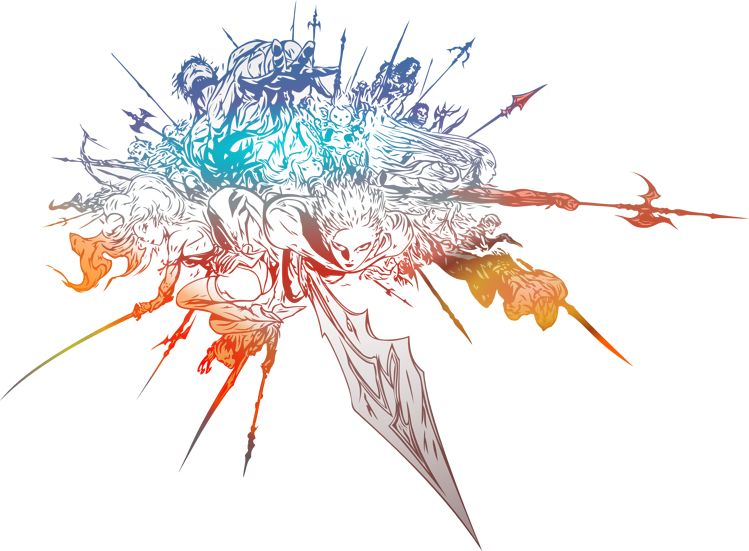
\includegraphics[width=\columnwidth]{./art/images/ff14.jpg}
%
\\\\\\
%
Em situações difíceis, herois podem ir além de seus limites e liberar habilidades poderosas, chamadas \accf{Quebra de Limite}.
Ao alcançarem o \accf{Nível~4}, os jogadores podem criar sua própria habilidade de Quebra de Limite.
Para usá-lo, o personagem tem que juntar 10 \accf{Pontos Limite~(PL)}, que serão consumidos ao ativar sua Quebra de Limite.
Cada jogador também escolhe um \accf{Modo Limite} para decidir sob quais circunstâncias seu personagem ganha PL, o que nunca excede 10 pontos.
Todos os Modos Limite disponíveis e suas condições d ganho de Pontos Limite estão na próxima página.
O MJ também pode permitir aos jogadores criarem suas próprias condições de Modo Limite.
A Quebra de Limite e o Modo Limite podem ser trocados a cada nível subsequente.
%
\ofpar\ofpar
%
\ofquote{"Quando um inimigo te irrita até o seu limite, você pode liberar um poder inimaginável."\\}{Cloud}
%
\ofpar
%
\ofboxwithtitle{Exemplo: Pontos Limite}{
	Vivi e seus amigos estão viajando em uma aeronave quando subitamente um mago hostil, chamado Valsa Negra, desce ao deque.
	O demônio causa KO a 5 passageiros imediatamente, usando uma poderosa magia de Raio. 
	Vivi selecionou o Modo Limite, Vingador, então ele ganha 10 pontos imediatamente ao assistir ao incidente.
	Ele jura se vingar e combater o monstro.
	Ele ativa sua Quebra de Limite, esvaziando sua Barra de Limite e recebendo poderosos benefícios de combate.
	A Quebra de Limite dá a Vivi e a seu grupo uma vantagem muito necessária na batalha que os permitem derrotar o poderoso inimigo em definitivo.
}
%
\newpage
%
Além de Modos Limite, todos os jogadores também ganham Pontos Limite nas seguintes situações: \ofrow
\ofbullet{3 PL após terminar uma batalha.}
\ofbullet{3 PL após acordar.}
\ofbullet{3 PL após usar um Talento.}
\ofbullet{10 PL após um aliado sofrer Ko e você for o último de pé.}
\ofbullet{10 PL após subir de Nível.}
\ofbullet{O MJ é encorajado a premiar PLs extras sempre que o personagem realiza um feito impressionante, heroico ou sempre que o grupo cumprir atividades ou missões importantes.}
%
\ofpar\\
%
\ofquote{"Vamos só atirar feito loucos e fazer um grande buraco, BOOM!"\\}{Selphie}
%
\ofpar
%
Quebra de Limite é usado da mesma maneira que Magia e Técnicas, mas sem custo de PM ou tempo de conjuração.
Você pode criar uma Quebra de Limite única ao escolher qualquer uma de suas magias ou técnicas como base.
Assim, adicione algumas melhorias e efeitos a fim de transformar a habilidade.
Cada efeito adicional aumenta o \accf{Grau~(GR)} de sua Quebra de Limite, que não pode exceder 5 pontos. 
Entretanto, não há benefício em ficar abaixo desse valor.
Por fim, escolha um novo nome para sua Quebra de Limite e visualize como ele é ao ser ativado.
Todas as possíveis melhorias que você possa usar para na criação, assim como o custo de Grau dela, estão listadas abaixo.
Você não pode escolher a mesma melhoria mais de uma vez, embora o MJ possa permitir outras opções além das listadas abaixo, atribuindo-lhes um Grau.
%
\ofpar\\
%
\ofboxwithtitle{Exemplo: Quebra de Limite}{
	Cloud, profissão Guerreiro, alcança o Nível 4, então ele pode criar sua própria Quebra de Limite.
	Ele escolhe sua habilidade Surrar como base, que permite ao usuário Atacar com menos precisão, garantindo um Acerto Crítico se acertar.
	Ele escolhe as seguintes melhorias até o Grau 5:
	\ofbullet{Mova-se até 3u antes ou depois de usar a habilidade.}
	\ofbullet{Ataques feitos durante a habilidade não podem ser evadidas.}
	\ofbullet{O dano causado ao alvo ignora DEF e RES.}
	\ofbullet{Alvos sofrem dano extra igual ao seu Nível atual.}
	Portanto, a nova habilidade o permite se reposicionar e então executar um Acerto Crítico, ignora a DEF e RES do alvo e causa 4 de dano extra. 
	Sendo uma Quebra de Limite, não há custo de PM ou tempo de conjuração.
	Cloud escolhe o nome Valente e o descreve da seguinte maneira:
	Você corre em direção ao alvo e antes de alcançá-lo, você salta no ar e executa um poderoso golpe de cima pra baixo. 
}
%
\clearpage
%
\oftable{p{0.22\columnwidth} p{0.06\columnwidth} p{0.65\columnwidth}}
{\accf{Modo Limite} & \accf{PL} & \accf{Condição}}
{
	Altruísta & 5 & Doe à caridade ou pessoa em necessidade. \ofrow
	Assaltante & 10 & Tenha uma rodada surpresa no combate. \ofrow
	Atleta & 5 & Malhe ou realize uma atividade física por pelo menos 1 hora. \ofrow
	Vingador & 4 & Um aliado que você vê sofre KO.\ofrow
	Traça & 5 & Leia ou estude por pelo menos 1 hora. \ofrow 
	Corajoso & 5 & Passe num teste com Desvantagem. \ofrow
	Covarde & 5 & Escape durante uma batalha.\ofrow
	Competitivo & 5 & Vença um jogo ou competição. \ofrow
	Criativo & 5 & Crie uma obra de arte.\ofrow
	Criminoso & 5 & Quebre a lei do local. \ofrow
	Culinária & 5 & Prepare e coma uma refeição gostosa.\ofrow
	Destemido & 5 & Ao fim da batalha seu PV está menos da metade.\ofrow
	Dominador & 5 & Ao fim da batalha seu PV está cheio. \ofrow
	Condutor & 5 & Conduza um veículo ou montaria por pelo menos 1 hora. \ofrow
	Elusivo & 2 & Evada-se de um ataque. \ofrow
	Explorador & 10 & Entre numa ruína, caverna, masmorra ou estrutura natural nova. \ofrow
	Ganancioso & 5 & Ganhe Gil ao completar tarefas.\ofrow
	%Pechinchador & 10 & Convença um mercador a dar um desconto ou pagar um preço maior por algo.\ofrow
	Útil & 5 & Crie ou repare um produto funcional. \ofrow
	Curandeiro & 4 & Remova KO de um aliado. \ofrow
	Solitário & 1 & seja escolhido por ultimo na ordem de turno de seu grupo. \ofrow
	Sortudo & 3 & Use um Dado de Fortuna. \ofrow
	Orador & 5 & Faça um discurso motivacional. \ofrow
	Pacifista & 5 & Evite o combate com sucesso. \ofrow
	Sombra & 5 & Esgueire-se por alguém sem ser notado.\ofrow
	Matador & 2 & Reduza um inimigo a 0 PV. \ofrow
	Sabotador & 2 & Inflija um Efeito de Estado em um ou mais inimigos. \ofrow
	Dorminhoco & 3 & Durma pelo menos 8 horas. \ofrow
	Espiritual & 4 & Realize um ritual ou prece religiosa. \ofrow
	Fornecedor & 1 & Use um Item.\ofrow
	Sociável & 2 & Tenha uma conversa com uma pessoa que não conheça.\ofrow
	Azarado & 4 & Falhe num teste com Vantagem. \ofrow
	Urbano & 10 & Entre numa vila, cidade pequena ou grande nova. \ofrow
	Vitimante & 5 & Sofra KO.\ofrow
	Andarilho & 5 & Ande a pé por pelo menos 1 hora. \ofrow
	Aquecimento & 1 & Use a habilidade na qual sua Quebra de Limite é baseada.
}
%
\newpage
%
\oftable{p{0.85\columnwidth} r}
{\accf{Efeito Adicional} & \accf{GR}}
{
	A habilidade ganha um tipo elemental que causa dano extra igual a metade de seu nível atual ao alvo. & +1 \ofrow
	Mude o tipo de dano causado entre Físico e Mágico. & +1 \ofrow
	Alvos sofrem dano extra igual ao seu nível atual. & +1 \ofrow
	Alvos recuperam PV igual ao seu nível atual. & +1 \ofrow
	A distância é aumentada em 3u. & +1 \ofrow
	Se os alvos tem de fazer um teste, o Quebra de Limite aumenta em 2. & +1 \ofrow
	Alvos se tornam Imunes a Efeitos de Estado à sua escolha por 3 rodadas. & +1 \ofrow
	Alvos recuperam PM igual ao seu nível atual. & +1 \ofrow
	Mova-se até 3u antes ou depois de usar uma habilidade. & +1 \ofrow
	Somente inimigos na área são afetados.  & +1 \ofrow
	Dano causado ignora a DEF e RES do alvo. & +1 \ofgap
	Dano causado ignora as Resistências do alvo. & +1 \ofgap
	A área alvo aumenta em 2u. & +2 \ofrow
	Recupere PM igual a duas vezes seu nível atual. & +2 \ofrow
	Empurre os alvos até 3u. & +2 \ofrow
	Tome a ação Defender após usar a habilidade.  & +2 \ofrow
	Efeitos com duração se estendem por mais 2 rodadas. & +2 \ofrow
	Alvos sofrem o Efeito de Estado escolhido por você, exceto KO, por 1 rodada. & +2 \ofrow
	Após usar a habilidade, faça um Ataque contra um alvo dentro do alcance. & +2 \ofrow
	Use a habilidade como reação sob condições específicas. Ex.: receba dano, a rodada termina, um inimigo entra ao seu alcance. & +2 \ofrow
	Use um item de seu inventário em adição. & +2 \ofrow
	O PM dos alvos é reduzido igual ao seu nível atual. & +2 \ofrow
	Ataques realizados por habilidades não podem ser evadidos. & +2 \ofrow
	Um aliado dentro de 3u pode usar uma habilidade conhecida no mesmo alvo sem custo adicional ou tempo de conjuração.  & +2 \ofrow
	Alvos sofrem dano extra igual a sua FOR ou MAG combinadas. & +2 \ofrow
	Alvos se tornam Imunes a Efeitos de Estado negativos por 3 rodadas. & +3 \ofrow
	Aja novamente após usar essa habilidade. & +3 \ofrow
	Crie um Campo à sua escolha que alcance até 3u ao redor do alvo e dure 3 rodadas. & +3 \ofrow
	Após usar a habilidade, ganhe AuFOR, AuMAG, AuDEF e AuRES por 3 rodadas. & +3 \ofrow
	Alvos ganham Resistência contra todos os tipos elementais por 3 rodadas. & +3
}
%
\clearpage
\ofsubsection{Summons}
%
\ofquote{"This battle is ours as much as anyone's. Cecil said so himself. And having some Eidolons along can't hurt, can it?"}{Rydia}\\\\
%

\includegraphics[width=\columnwidth]{./art/images/ff10.jpg}\\\\
%
\accf{Summons}, also known as Espers or Eidolons, are extraordinarily powerful magical beings that exist beyond the realm of humans and monsters.
They reside within their own plane of existence, but can manifest themselves in the real world when necessary.
In rare cases, when a Summon is impressed by an outstanding mortal, it will lend its powers to aid his or her cause.
When reaching \accf{Level~5} each player chooses one Summon that bonds with their character.
The bond grants a permanently available supportive effect, as well as a summon ability that can be activated using an action in combat. 
All summon abilities have a cast time of 1 round and cost 10\% of your current HP and MP to use.
However, this cost cannot fall below a minimum of 1 HP and 1 MP.
All available Summons are listed below.
%
\vfill
%
\ofsummon{Odin}{./art/esper/odin.jpg}
{You can perform a short ritual to summon Odin's horse, Sleipnir. When riding on its back, you are twice as fast as usual. Sleipnir disappears whenever it takes any damage or when you dismiss it.}
{Choose any enemy on the battlefield. He makes a DC~8 check and suffers KO upon failure. If he succeeds or is Immune to this effect, the target suffers physical damage equal to 3 times your current Level.}
{STR +2, DEF +1}
%
\newpage
%
\ofsummon{Alexander}{./art/esper/alexander.jpg}
{Whenever you use an Item, you can additionally increase the target's HP by an amount equal to your current Level.}
{All enemies on the battlefield suffer holy damage equal to 2 times your current Level. In addition, all affected targets suffer Immobile for 1 round.}
{DEF +1, MaxHP +10}
%
\vfill
%
\ofsummon{Gilgamesh}{./art/esper/gilgamesh.jpg}
{Whenever you choose the Re-Equip action, you gain EnSTR for 2 rounds.}
{For 1 round, whenever you or an ally performs a successful Attack you always score a Critical Hit.}
{STR +2, MaxHP +5}
%\\
\vfill
%
\ofsummon{Ifrit}{./art/esper/ifrit.jpg}
{You can always conjure a small flame in a location within 10u of you. It does not deal any damage, but can for example be used to ignite wood.}
{You create a Hot Field centered around you, that reaches 3u and lasts for 5 rounds. The field follows you, but does not affect you.}
{STR +1, MaxHP +10}
%
\clearpage
%
\ofsummon{Shiva}{./art/esper/shiva.jpg}
{You can freeze any liquid that is smaller than 1u in every dimension with your touch. In addition, you can create a solid path of ice over a lake or river up to a length of 50u.}
{Choose any enemy on the battlefield. He and anyone within 3u of him suffer ice damage equal to your 2 times your current Level. In addition, you create a Slippery Field in the targeted area, that lasts for 3 rounds.}
{MAG +2, RES +1}
%
\vfill
%
\ofsummon{Titan}{./art/esper/titan.jpg}
{Whenever you are in a natural environment such as a forest or cave, you gain Resilience against all elemental damage except dark and holy.}
{You grow 3 times in size for the next 3 rounds, accordingly you take up 3u in diameter when viewed from above. As long as this effect is active, you gain EnDEF and EnRES.}
{DEF +2, STR +1}
%
\vfill
%
\ofsummon{Magus Sisters}{./art/esper/magus.jpg}
{Choose 2 allies. The three of you can communicate telepathically over a distance of up to 100u. You can change your chosen allies when you go to sleep.}
{You can take 3 actions on your next turn.}
{MaxHP +5, MaxMP +10}
%
\vfill
%
\ofsummon{Phoenix}{./art/esper/phoenix.jpg}
{Whenever you wake up from sleep or are revived from KO, you gain a temporary shield that breaks upon taking total damage equal to your current Level.}
{Remove KO from all allies on the battlefield and increase their HP by 1.}
{MaxMP +5, RES +2}
%
\vfill
%
\ofsummon{Bahamut}{./art/esper/bahamut.jpg}
{Whenever you fall from any height, you can gracefully glide down to avoid damage. In addition, you can levitate 1u above ground for a distance up to 15u. While levitating you can move half as fast as usual.}
{Choose any enemy on the battlefield. After 3 rounds, the target suffers fire damage equal to 5 times your current Level.}
{STR +2, MAG +1}
%
\vfill
%
\ofsummon{Siren}{./art/esper/siren.jpg}
{You have Advantage on all checks related to deescalating a situation through speech.}
{You create a noise-absorbing field that follows you and reaches up to 10u for 15 minutes. Nobody outside of the field can hear any noise that is created inside of it.}
{MAG +1, DEF +1, RES +1}
%
\clearpage
%
\ofsummon{Ramuh}{./art/esper/ramuh.jpg}
{You can send out barely perceptible electric pulses, which travel through solid structures up to a distance of 25u and allow you to detect the presence of nearby living beings.}
{You conjure a storm  that covers the entire battlefield and acts as an Obscure Field. It lasts for 3 rounds and does not affect you.}
{MAG +1, MaxMP +10}
%
\vfill
%
\ofsummon{Leviathan}{./art/esper/leviathan.jpg}
{You can stay underwater indefinitely. In addition, you gain permanent Resilience against water damage.}
{From the point you are standing, you conjure a stream of water that is 5u wide, reaches up to 10u and lasts for 3 rounds. It acts as a Slow Field that only affects enemies.}
{MAG +1, DEF +2}
%
\vfill
%
\ofsummon{Asura}{./art/esper/asura.jpg}
{Whenever you use a Fortune Die, you can replace two dice in your roll with the value removed from the pool.}
{Roll 1d. You and all of your allies gain one of the following effects based on the result.\\ 1-2: regain HP equal to 2 times your current Level.\\ 3-4: EnDEF and EnRES for 3 rounds,\\ 5-6: Haste for 3 rounds.}
{STR +1, MAG +1, DEF +1}
%
\newpage
%
\ofsummon{Carbuncle}{./art/esper/carbuncle.jpg}
{Whenever you want, you can make one of your hands glow in a bright red color. The emitted light allows you to see a distance of up to 20u in darkness.}
{You and all of your allies gain a magical shield that reflects the effect of the next spell that targets you back to its caster. This shield does not stack and lasts up to 3 rounds if not activated.}
{RES +1, MaxMP +10}
%
\vfill
%
\ofsummon{Diabolos}{./art/esper/diabolos.jpg}
{While you are asleep, you still have a strong sense of your surroundings. Therefore, you cannot be surprised by an ambush at night.}
{All enemies on the battlefield suffer damage equal to 10\% of their maximum HP. The damage dealt ignores the targets' DEF and RES.}
{STR +1, MaxMP +10}
%
\vfill
%
\ofsummon{Atomos}{./art/esper/atomos.jpg}
{Using an action, you can pull an object to yourself that is within 10u and less than half your size.}
{You conjure a portal that lasts for 1 minute (6 rounds) and teleports everyone who steps through it to another location. The portal can lead to any location in which you have used this ability before.}
{MAG +1, MaxMP +10}
%
\defaultgeometry
\clearpage
\ofsection{Game Master}
%
\ofquote{"Tough... Don't blame us. Blame yourself or God."\\}{Delita}\\\\
%

\includegraphics[width=\columnwidth]{./art/images/ff4.jpg}
%
\vfill
%
The \accf{Game Master} creates the setting of the adventure and takes the role of all non-player characters.
Furthermore, the GM describes the environment around the protagonists and decides the outcomes of most actions by applying the rules of the game. 
However, unlike the players, the GM is not strictly bound by rules and may make his own rulings when necessary.
There is no single way to be a successful GM and we encourage you adopt a style that brings enjoyment to both you and the players.
%
\vfill
%
Accordingly, this chapter does not focus on presenting rules or advice.
Instead, it is a collection of optional \accf{supplements}, that you can either use directly or regard as examples for creating your own content.
These supplements not only give a glimpse into the various aspects of game mastering, but also show different directions that you can take as a GM. 
The present modules can be broadly split into two categories: \accf{prepared content} and \accf{optional rules}.
The former provide you with world building blocks such as adventures, settings and monsters that are self-contained and extensible.
The latter present you examples to customize the rules to your preferences by changing or adding to existing ones.
While the prepared content is well suited for beginners, we recommend to consider optional rules once you have gathered some experience.
All available supplements are listed in the following, together with a short synopsis for each one.
%
\newpage
%
{\large\accf{Prepared Content:}}
%
\vfill
%
\accf{Bestiary:} discusses guidelines for creating monsters and combat encounters.
Also includes a collection of prepared enemies that you can use directly.
%
\vfill
%
\accf{Chaos in Cornelia:} a short adventure in which the party has to save a kidnapped princess. 
Contains diverse content including combat, roleplaying and exploration. Highly recommended for beginners!
%
\vfill
%
\accf{Tomb of Raithwall:} a short adventure in which the party has to recover an artifact from a dangerous tomb.
Focused on exploring an environment full of traps and adversaries. 
%
\vfill
%
\accf{Maria \& Draco:} a single-session adventure in which the party has to ensure the success of an opera performance.
Encourages a light-hearted narrative with interesting roleplaying moments.
%
\vfill
%
\accf{Siege of Dollet:} a single-session adventure in which the party has to pass a test to join an elite mercenary force.
Encourages an action packed narrative with lots of combat.
%
\vfill
%
\accf{Gold Saucer:} an amusement park where the party can blow off steam and win rare prizes. 
Focused on recreating the games and competitions in the park.  
%
\vfill
%
\accf{Ivalice Worldbook:} a very detailed document that fleshes out the world of Ivalice, including its history and geography.
You can create various adventures in this world or use it as an example for creating a detailed setting.
%
{\large\ofpar\ofrow\accf{Optional Rules:}}
%
\vfill
%
\accf{Additional Rules:} minor rule changes and additions that help you to customize the feeling of the game.
%
\vfill
%
\accf{Races:} rules and examples for incorporating different humanoid races in your world. 
This provides additional character creation options for players, but can also help you to create a more interesting game world.
%
\vfill
%
\accf{Chocobo:} rules for incorporating bird-like creatures called Chocobos as full-fledged party members.
Players can raise Chocobos, use them as mounts and fight alongside them in combat.
%
\vfill
%
\accf{Triple Triad:} rules for a fun card game, allowing the party to collect and play cards.
Well suited if you are looking quick and simple side-activity for the party.
%
\vfill
%
\accf{Blitzball:} rules for a fun team-based sports game similar to water polo.
Well suited if you are looking for a more elaborate side-activity for the party.
%
\clearpage
\ofsubsection{Bestiário}
%
\ofquote{"Ao longo do tempo, o mundo encontra maneiras novas e empolgantes de matar um homem.}{Balthier}
%
\\\\
%

\includegraphics[width=\columnwidth]{./art/images/ff6.jpg}
%
\vfill
%
\accf{Encontros de combate} podem ocorrer em várias situações diferentes, como por exemplo, o grupo tenta fugir de uma gangue de bandidos ou terão que enfrentar o grande vilão num confronto épico.
O combate é geralmente uma questão de vida ou morte e pode tomar uma parte significante do tempo de jogo. 
No entanto, nem sempre tem que ser uma luta até a morte, pois o grupo pode tentar soluções alternativas, como negociar ou escapar. 
Durante o combate, o MJ representa o papel de todos os adversários, aplicando as regras de combate a eles, embora possa manter informações cruciais secretas, como atributos e rolagens de dados dos inimigos.
Enquanto jogando como um grupo inimigo, tente tomar decisões da perspectiva deles, sem usar seu próprio conhecimento.
Além disso, também é útil usar auxílio visual, como mapas, a fim de acompanhar o desenvolver no campo de batalha.
As \accf{Recompensas de combate} normalmente fazem uma grande parte da riqueza do grupo e a tabela abaixo oferece orientações aproximadas a depender do nível do grupo.
Um grupo com Gil insuficiente não pode pagar por itens essenciais, mas aquele com bastante, pode evitar muitas consequências.
As recompensas nem sempre são em Gil, podem ser equipamentos, itens ou materiais de valor parecido e por padrão, são divididos entre todos os membros do grupo.
%
\vfill
%
\oftable{p{0.3\columnwidth} p{0.7\columnwidth}}
{\accf{Nível} & \accf{Recompensa de combate por jogador}}
{
	1 & 200G \ofrow
	2 & 300G \ofrow
	3 & 500G \ofrow
	4 & 800G \ofrow
	5 & 1.000G \ofrow
	6 & 1.200G \ofrow
	7 & 1.500G \ofrow
	8 & 2.000G \ofrow
	9 & 2.500G \ofrow
	10 & 3.000G
}
%
\newpage
%
A dificuldade dos encontros de combate variam muito e você pode adequá-los a depender do contexto e das preferências de seu grupo.
Por outro lado, o combate é a causa mais comum da morte de personagens, então se recomenda cuidado a fim de evitar surpresas inesperadas.
Mesmo assim, normalmente é desejável que o combate seja um desafio considerável.
Alcançar um equilíbrio satisfatório pode exigir algum esforço, porque a dificuldade do encontro depende de vários fatores:
Primeiro, as circunstancias da batalha podem afetar consideravelmente esse equilíbrio.
Como por exemplo, os jogadores estarão em grande desvantagem ao já terem sidos afetados por batalhas anteriores no mesmo dia ou quando o grupo adversários consegue uma rodada surpresa.
Além do mais, a composição e preparação de ambos os grupos afetam bastante o resultado.
Como por exemplo, um grupo de apenas lutadores físicos não terão problemas com inimigos comuns, o que pode não se repetir com inimigos que atacam à distância e aplicam Efeitos de estado.
Por fim, a experiência de sue grupo também terão grande impacto.
Como por exemplo, os jogadores novatos podem perder oportunidades, enquanto aqueles com muita experiência frequentemente sacam truques de suas mangas.
Contudo, infelizmente não é possível determinar as regras que se aplicam a cada grupo e situação.
Mesmo assim, pode-se discutir algumas orientações aproximadas e regras de ouro que podem ser consideradas.
Note que geralmente erramos pela precaução, com conselhos e conteúdo preparado, e você é encorajado a modificá-los em caso de não servirem adequadamente. 
%
\ofpar
%
Ao montar um grupo inimigo, recomenda-se ter um números de integrantes similar ao grupo dos jogadores e em que a força deles seja parecida.
Grandes hordas de inimigos fracos provavelmente vão sobrepujar o grupo, enquanto aqueles solitários, raramente terão alguma chance.
Uma configuração equilibrada garante que dois recursos importantes sejam parecidos: o número e força das ações de combate de ambos os lados.
Para medira a força de um inimigo, use Níveis que podem ser comparados aos dos jogadores.
Como por exemplo, se um grupo tem 4 personagens, o grupo adversário deve conter a mesma quantidade e nível.
o próximo passo é usar as seguintes orientações para determinar seus atributos:
Para cada nível, o inimigo ganha 6 \accf{Pontos de atributo}, dos quais cada ponto são iguais ao PV/PM~+5 ou FOR/MAG/DEF/RES~+1.
A AGI deles dever variar de 1 e 4, do contrário ataques comuns serão inefetivos.
Assim como os personagens, os inimigos podem usar Magias e Técnicas, além de habilidades Passivas e de Reação.
No entanto, recomenda-se manter a quantidade de habilidades inimigas baixa a fim de permitir decisões rápidas em combate.
Embora, sinta-se livre para lhes dar acesso a habilidades únicas ou exóticas.
Considere qualquer equipamento nos atributos totais de um inimigo e para armas, atribua o Dano do nível de equipamento de acordo com o nível dele.
Você também pode adicionar mais profundidade aos inimigos ao atribuir resistências e fraquezas elementais ou imunidades a estados de efeito.
Durante o combate, você pode dar dicas sutis sobre estas especialidades aos jogadores, ao narrar as ações de combate e seus efeitos.
%
\vfill
%
Em alguns casos, pode ser mais interessante criar um grupo adversário que é desbalanceado em número.
Como por exemplo, você pode querer que o grupo enfrente uma horda de inimigos fracos ou um único inimigo forte, o tal \accf{Chefe}.
Portanto, nesses casos, a força dos inimigos será diferente das dos jogadores.
No caso do grupo de inimigos superam em número o dos jogadores, recomenda-se usar inimigos de níveis mais baixo em que a soma de todos os níveis se igualem ou se aproximem em ambos os grupos.
No caso do inimigo ser superado em número, eles precisam de mais força para lidar com vários adversários.
Além de atributos aumentados, \accf{Características de chefe} podem ajudar aos seus Chefes a compensar a falta de aliados.
Características de chefe são habilidades especiais particularmente fortes, que garantem aos inimigos ações adicionais e durabilidade.
Recomenda-se as seguintes orientações para equilibrar um chefe: para cada adversário extra com que ele é capaz de lidar, dê 2 Pontos de atributo extras por nível assim como uma característica de chefe.
Como por exemplo, um chefe de Nível 5, lutando contra um grupo de 4 personagens devem ter pelo menos \mbox{5 x (6 + 3 x 2) = 60 Pontos de atributo} e 3 características de chefe.
Uma lista delas está ao lado.
%
\vfill
%
Os seguintes tipos de configuração de grupo de inimigos irregularmente equilibrados são usadas normalmente:
\ofrow
\accf{Chefe único:}
Um inimigo poderoso sozinho, pode ser um exemplo do vilão principal.
Ue as orientações mencionadas acima para garantir que o chefe pode lidar com muitos jogadores.
Um chefe único também se beneficia bastante de especialidades extras, tais quais interações especiais com o ambiente.
Esta variante é o equilíbrio mais complicado, então é recomendado outras sempre que possível.
\ofrow
\accf{Conselho de chefes:} 
O grupo de inimigos consistem de pequeno grupo de Chefes, geralmente de 2 a 3 com cada um sendo equivalente em força, mas mais forte do que um personagem.
Normalmente,suas forças se complementam, por exemplo, um Chefe pode se forcar na ofensiva enquanto os outros se destacam em cura.
\ofrow
\accf{Chefe com lacaios:} 
Este chefe tem vários inimigos comuns trabalhando com eles, por exemplo, um Necromante levantando sua horda de mortos-vivos.
Neste caso, o chefe é mais forte do que o jogador enquanto que os lacaios, mas fracos.
\ofrow
\accf{Chefe múltiplas-partes:} 
Este tipo de chefe é representado por várias partes.
Cada parte é construída como um inimigo com seu próprio turno, atributos e habilidades, mas todas elas só podem se mover em conjunto uma vez.
Geralmente, uma das partes age como o núcleo, ao morrer, todas as outras morrem com ela.
É comum que o núcleo também tenha proteção extra e a habilidade de regenerar outras partes que tenham sofrido de KO.
\ofrow
\accf{Horda inimiga:} 
Um grande grupo de inimigos comuns, geralmente do mesmo tipo e de nível menor do que os jogadores.
No entanto, aconselha-se contra um grupo que supere os jogadores em 2 para 1, por exemplo, se tiver 4 deles, eles não devem enfrentar mais do que 8 inimigos de uma vez.
%
\newpage
%
\oftable{p{0.24\columnwidth} p{0.7\columnwidth}}
{\accf{Características de Chefe} & \accf{Efeito}}
{
	Auto-Acerto & Ataque acertam sempre, mas não geram Críticos. \ofrow
	Auto-Oscilar & Permanentemente Oscilando. \ofrow
	Auto-Acelerar & Permanentemente Acelerado. \ofrow
	Auto-Regenerar & Permanentemente Regenerando. \ofrow
	Auto-Apressar & tenha 2 turnos por rodada. \ofrow
	Superimune & Imunidade permanente a todos os Estados de efeito negativos. \ofrow
	Revidar & Uma vez por rodada, ao sofrer dano, pode atacar o agressor, se ele estiver ao alcance. \ofrow
	TC-0 & O tempo de conjuração de magias e técnicas é 0r.\ofrow
	Golpe duplo & Com cada ataque, pode alvejar 2 alvos diferentes ao alcance. \ofrow
	Desvanecer & Pode se evadir de magias assim como de ataques. \ofrow
	Ataque final & Quando sofrer KO, pode agir antes de cair inconsciente. \ofrow
	Reverter & Uma vez por rodada, pode repetir a rolagem de um dado após a rolagem. \ofrow 
	Retaliar & Uma vez por rodada, ao sofrer dano, pode usar uma habilidade contra o agressor ao alcance. \ofrow
	Surtar & Ao ter PV reduzido abaixo da metade, ganhe AuFOR, AuDEF, AuMAG e AuRES até o fim da batalha. \ofrow
}
%
\vfill
%
\accf{Gladio: "Então, este espadachim..." \\ Cor: "Ele é um mestre das lâminas. Ahm, esperava algo mais profundo?"}
%
\vfill
%
Diferente dos jogadores, os \accf{Monstros} são outro tipo comum de adversários que o grupo enfrentam em combate.
Eles são seres selvagens que vivem em seu habitat natural, ao contato com o grupo é comum se sentirem ameaçados e atacar.
Monstros diferentes, com frequência, trabalham contra hostis e o grupo pode cruzar com alguns inteligentes, que possuem objetivos complexos.
Em geral são parte ou causa de um grande conflito e por isso, sua aventura pode ter vários monstros na trama principal.
Comparado aos personagens, eles também podem variar bastante em tamanho e aparência.
Eles são classificados como Médio~(\accf{M}), se tiverem cerca de 1u de diâmetro, Grande~(\accf{G}), se tiverem mais do que 2u e Pequeno~(\accf{P}), se tiverem menos do que 0.5u. Monstros não usam armas e armaduras comuns, mas eles têm partes similares integradas aos seus corpos, que seguem as mesmas regras.
As páginas seguintes incluem vários monstros de níveis diferentes preparados. Você deve usá-los como apresentado, mas também é encorajado a se modificar cada um deles a fim de se ajustar à necessidade ou use os como exemplos para criar os seus próprios.
%
\clearpage
%
%
%
%%%%%%%%%%%%%%%%%%%%%%%%%%%%%%%L1%%%%%%%%%%%%%%%%%%%%%%%%%%%%%%%%%%%%%%%%%
%
\ofmonster{Goblin}{1}{
\includegraphics[width=0.2\columnwidth]{./art/monsters/goblin.jpg}}
{
	PV: & \hfill 12 & PM: & \hfill 0\\
	FOR: & \hfill 2 & DEF: & \hfill 1 \\
	MAG: & \hfill 0 & RES: & \hfill 1 \\
	AGI: & \hfill 3 & Tamanho: & \hfill M\\
}
{\accf{Faca}: 1d Dano \hfill \accf{Imune}:\immobile}
{}
%
\vfill
%
\ofmonster{Esqueleto}{1}{
\includegraphics[width=0.17\columnwidth]{./art/monsters/skeleton.jpg}}
{
	PV: & \hfill 11 & PM: & \hfill 0\\
	FOR: & \hfill 2 & DEF: & \hfill 2 \\
	MAG: & \hfill 0 & RES: & \hfill 0 \\
	AGI: & \hfill 2 & Tamanho: & \hfill M \\   
}
{\accf{Espada}: 1d Dano \hfill \accf{Fraco}:\fire\holy}
{\mpassive{Morto-vivo}{Zumbi permanentemente.}}
%
\vfill
%
\ofmonster{Mandrágora}{1}{
\includegraphics[width=0.14\columnwidth]{./art/monsters/mandragora.jpg}}
{
	PV: & \hfill 10 & PM: & \hfill 18\\
	FOR: & \hfill 0 & DEF: & \hfill 0 \\
	MAG: & \hfill 0 & RES: & \hfill 1 \\
	AGI: & \hfill 2 & Tamanho: & \hfill P\\
}
{\accf{Cabeçada}: 1d Dano \hfill \accf{Fraco}:\lightning}
{\mspell{Dormir}{6}{0r}{Único}{3u}{O alvo faz um teste de DF 8 ou fica Adormecido por 43 rodadas.}{\sleep}}
%
\vfill
%
\ofmonster{Tarântula}{1}{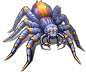
\includegraphics[width=0.25\columnwidth]{./art/monsters/tarantula.jpg}}
{
	PV: & \hfill 10 & PM: & \hfill 16\\
	FOR: & \hfill 1 & DEF: & \hfill 0 \\
	MAG: & \hfill 0 & RES: & \hfill 0 \\
	AGI: & \hfill 3 & Tamanho: & \hfill P\\
}
{\accf{Mordida}: 1d Dano \hfill \accf{Fraco}:\fire \hfill \accf{Imune}:\poison}
{\mtech{Teia}{4}{0r}{Único}{5u}{O alvo faz um teste de DF 8 ou fica Imóvel por 1 rodada.}{\immobile}}	
%
\vfill
%
\ofmonster{Bandersnatch}{1}{
\includegraphics[width=0.27\columnwidth]{./art/monsters/bandersnatch.jpg}}
{
	PV: & \hfill 10 & PM: & \hfill 6\\
	FOR: & \hfill 2 & DEF: & \hfill 1 \\
	MAG: & \hfill 0 & RES: & \hfill 0 \\
	AGI: & \hfill 3 & Tamanho: & \hfill M\\
}
{\accf{Garra}: 1d Dano \hfill \accf{Fraco}:\ice}
{\mtech{Mordida}{2}{0r}{Único}{1u}{Ataque o alvo, se acertar, cause dano e ignore a DEF dele.}{}}	
%
\vfill 
%
%%%%%%%%%%%%%%%%%%%%%%%%%%%%%%%L2%%%%%%%%%%%%%%%%%%%%%%%%%%%%%%%%%%%%%%%%%
%
%
\ofmonster{Sahagin}{2}{
\includegraphics[width=0.17\columnwidth]{./art/monsters/sahagin.jpg}}
{
	PV: & \hfill 16 & PM: & \hfill 24\\
	FOR: & \hfill 1 & DEF: & \hfill 0 \\
	MAG: & \hfill 2 & RES: & \hfill 1 \\
	AGI: & \hfill 3 & Tamanho: & \hfill M\\
}
{\accf{Lança}: 1d Dano \hfill \accf{Resistente}:\water \hfill \accf{Fraco}:\lightning}
{\mspell{Água}{6}{0r}{Único}{4u}{Cause 2d de dano de Água ao alvo.}{\water}}
%
\newpage
%
\ofmonster{Basilisco}{2}{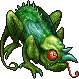
\includegraphics[width=0.2\columnwidth]{./art/monsters/basilisk.jpg}}
{
	PV: & \hfill 17 & PM: & \hfill 16 \\
	FOR: & \hfill 2 & DEF: & \hfill 2 \\
	MAG: & \hfill 0 & RES: & \hfill 1 \\
	AGI: & \hfill 3 & Tamanho: & \hfill M\\
}
{\accf{Lambida}: 1d Dano \hfill \accf{Resistente}:\earth \hfill \accf{Fraco:}\water}
{\mpassive{Toque de pedra}{Ao acertar um ataque, o alvo faz um teste de DF 7 ou fica Imóvel por 3 rodada.}}
%
\vfill
%
\ofmonster{Carniçal}{2}{
\includegraphics[width=0.18\columnwidth]{./art/monsters/ghoul.jpg}}
{
	PV: & \hfill 18 & PM: & \hfill 20\\
	FOR: & \hfill 2 & DEF: & \hfill 1 \\
	MAG: & \hfill 1 & RES: & \hfill 2 \\
	AGI: & \hfill 2 & Tamanho: & \hfill M\\
}
{\accf{Garra}: 1d Dano \hfill \accf{Fraco}:\fire\holy \hfill \accf{Resistente}:\ice}
{	
	\mtech{Modida zumbi}{3}{0r}{Única}{1u}{O alvo recebe 1d de dano e faz um teste de DF 8, se falhar, fica Zumbi por 5 rodadas.}{\zombie}		
	\mpassive{Morto-vivo}{Zumbi permanentemente.}
}
%
\vfill
%
\ofmonster{Cocatriz}{2}{
\includegraphics[width=0.2\columnwidth]{./art/monsters/cockatrice.jpg}}
{
	PV: & \hfill 15 & PM: & \hfill 16\\
	FOR: & \hfill 3 & DEF: & \hfill 1 \\
	MAG: & \hfill 0 & RES: & \hfill 2 \\
	AGI: & \hfill 3 & Tamanho: & \hfill M\\
}
{\accf{Bico}: 1d Dano \hfill \accf{Fraco}:\lightning}
{\mspell{Cegar}{6}{0r}{Único}{3u}{O alvo faz um teste de DF 8 ou fica Cego por 3 rodadas.}{\blind}}
%
\vfill
%
\ofmonster{Coeurl}{2}{
\includegraphics[width=0.23\columnwidth]{./art/monsters/coeurl.jpg}}
{
	PV: & \hfill 20 & PM: & \hfill 15\\
	FOR: & \hfill 2 & DEF: & \hfill 1 \\
	MAG: & \hfill 0 & RES: & \hfill 2 \\
	AGI: & \hfill 3 & Tamanho: & \hfill M\\
}
{\accf{Garra}: 1d Dano}
{\mtech{Raio d energia}{5}{0r}{Único}{5u}{O alvo faz um teste de DF 8 ou fica Imóvel por 3 rodadas.}{\immobile}}
%
\vfill
%
%
%%%%%%%%%%%%%%%%%%%%%%%%%%%%%%%L3%%%%%%%%%%%%%%%%%%%%%%%%%%%%%%%%%%%%%%%%%
%
%
% 
\ofmonster{Arimã}{3}{
\includegraphics[width=0.25\columnwidth]{./art/monsters/ahriman.jpg}}
{
	PV: & \hfill 20 & PM: & \hfill 24\\
	FOR: & \hfill 2 & DEF: & \hfill 1 \\
	MAG: & \hfill 0 & RES: & \hfill 4 \\
	AGI: & \hfill 4 & Tamanho: & \hfill P\\
}
{\accf{Feixe}: 1d Dano, 3u Alcance}
{\mtech{Onda de choque sinistra}{6}{0r}{Única}{3u}{O alvo faz um teste de DF 8 ou sofre 2d de dano e fica Mudo por 3 rodadas.}{\silence}}
%
\clearpage
%
\ofmonster{Abelha assassina}{3}{
\includegraphics[width=0.17\columnwidth]{./art/monsters/killerbee.jpg}}
{
	PV: & \hfill 20 & PM: & \hfill 18 \\
	FOR: & \hfill 3 & DEF: & \hfill 1 \\
	MAG: & \hfill 0 & RES: & \hfill 3 \\
	AGI: & \hfill 3 & Tamanho: & \hfill P\\
}
{\accf{Ferrão}: 1d Dano \hfill \accf{Imune}:\poison}
{\mpassive{Veneno}{Cada alvo que rolar abaixo de 6 ao se evadir contra seu ataque, fica Envenenado por 3 rodadas.}}
%
\vfill
%
\ofmonster{Pudim azul}{3}{
\includegraphics[width=0.3\columnwidth]{./art/monsters/flan.jpg}}
{
	PV: & \hfill 15 & PM: & \hfill 30\\
	FOR: & \hfill 0 & DEF: & \hfill 4 \\
	MAG: & \hfill 5 & RES: & \hfill 1 \\
	AGI: & \hfill 1 & Tamanho: & \hfill M\\
}
{\accf{Pancada}: 1d Dano \hfill \accf{Resistente}:\ice \hfill \accf{Fraco}:\fire }
{\mspell{Nevasca}{4}{0r}{Único}{3u}{Cause 2d de dano de Gelo ao alvo. }{\ice}}
%
\vfill
%
\ofmonster{Bomba}{3}{
\includegraphics[width=0.23\columnwidth]{./art/monsters/bomb.jpg}}
{
	PV: & \hfill 25 & PM: & \hfill 15\\
	FOR: & \hfill 3 & DEF: & \hfill 2 \\
	MAG: & \hfill 2 & RES: & \hfill 1 \\
	AGI: & \hfill 3 & Tamanho: & \hfill M\\
}
{\textbf{Pancada}: 1d Dano \hfill \textbf{Resistente}:\fire \hfill \textbf{Fraco}:\ice }
%{}
{\mtech{Auto-Destruição}{15}{1r}{2u}{Você}{Cause KO em si mesmo para causar 4d de dano de fogo a todos dentro da área.}{\fire}}
%
%\ofmonster{Death Claw}{3}{
\includegraphics[width=0.25\columnwidth]{./art/monsters/deathclaw.jpg}}
%{
%	HP: & \hfill 26 & MP: & \hfill 15\\
%	STR: & \hfill 2 & DEF: & \hfill 2 \\
%	MAG: & \hfill 0 & RES: & \hfill 1 \\
%	AGI: & \hfill 3 & Size: & \hfill M\\
%}
%{\accf{Claw}: 1d DMG}
%{\mtech{Grapple}{5}{0r}{Single}{2u}{The target becomes grappled and at the start of each turn he can make a DF~8 check to free himself. While grappled, the target suffers Immobile and an additional 1d damage for each failed attempt to free himself.}{}}
%
\vfill
%
\ofmonster{Feiticeiro}{3}{
\includegraphics[width=0.23\columnwidth]{./art/monsters/sorcerer.jpg}}
{
	PV: & \hfill 25 & PM: & \hfill 50\\
	FOR: & \hfill 0 & DEF: & \hfill 1 \\
	MAG: & \hfill 3 & RES: & \hfill 2 \\
	AGI: & \hfill 2 & Tamanho: & \hfill M\\
}
{\accf{Raio de energia}: 1d Dano, 3u Alcance \hfill \accf{Imune:}\silence\demag}
{
	\mspell{Silêncio}{6}{0r}{Único}{5u}{O alvo faz um teste de DF 8 ou fica Mudo por 3 rodadas.}{}
	\mspell{drenar}{8}{0r}{Único}{4u}{Reduz o PV do alvo em 1d e aumente o seu na mesma quantidade.}{}
}
%
\vfill
%
%%%%%%%%%%%%%%%%%%%%%%%%%%%%%%%L4%%%%%%%%%%%%%%%%%%%%%%%%%%%%%%%%%%%%%%%%%
%
%
\ofmonster{Formiga-leão}{4}{
\includegraphics[width=0.28\columnwidth]{./art/monsters/antlion.jpg}}
{
	PV: & \hfill 45 & PM: & \hfill 24\\
	FOR: & \hfill 2 & DEF: & \hfill 3 \\
	MAG: & \hfill 0 & RES: & \hfill 1 \\
	AGI: & \hfill 3 & Tamanho: & \hfill M\\
}
{\accf{Mordida}: 2d Dano \hfill \accf{Resistente}:\earth}
{\mtech{Tempestade de areia}{8}{0r}{3u}{Você}{Todos os inimigos na área sofrem 2d de dano de Terra e ficam Cegos por 1 rodada.}{\earth \blind}}
%
\newpage
%
\ofmonster{Diabrete}{4}{
\includegraphics[width=0.17\columnwidth]{./art/monsters/imp.jpg}}
{
	PV: & \hfill 30 & PM: & \hfill 40 \\
	FOR: & \hfill 2 & DEF: & \hfill 1 \\
	MAG: & \hfill 5 & RES: & \hfill 4 \\
	AGI: & \hfill 4 & Tamanho: & \hfill P\\
}
{\accf{Garra}: 2d Dano \hfill \accf{Imune:}\sleep \hfill \accf{Resistente}:\dark}
{	
	\mspell{Confusão}{10}{0r}{Único}{5u}{
		O alvo faz um teste de DF 8 ou você toma o seu controle no próximo turno dele. 
		Comende-o a se mover e atacar qualquer alvo à sua escolha, incluindo a si mesmo.
	}{}	
}
%
\vfill
%
\ofmonster{Minotauro}{4}{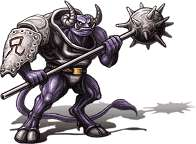
\includegraphics[width=0.3\columnwidth]{./art/monsters/minotaur.jpg}}
{
	PV: & \hfill 40 & PM: & \hfill 24 \\
	FOR: & \hfill 3 & DEF: & \hfill 2 \\
	MAG: & \hfill 0 & RES: & \hfill 1\\
	AGI: & \hfill 2 & Tamanho: & \hfill M\\
}
{\accf{Mangual}: 2d Dano \hfill \accf{Resistente}:\earth\fire}
{
	\mtech{Quebra-chão}{6}{0r}{3u (linha)}{Você}{Todos na área sofrem 3d de dano de Terra. }{\earth}	
	\mreaction{Reforçar}{Enquanto seu PV estiver abaixo da metade, ganhe AuFOR.}
}
%
\vfill
%
\ofmonster{Fantasma}{4}{
\includegraphics[width=0.2\columnwidth]{./art/monsters/ghost.jpg}}
{
	PV: & \hfill 35 & PM: & \hfill 50 \\
	FOR: & \hfill 2 & DEF: & \hfill 1 \\
	MAG: & \hfill 0 & RES: & \hfill 0 \\
	AGI: & \hfill 2 & Tamanho: & \hfill M\\
}
{\accf{Mordida}: 2d Dano \hfill \accf{Resistente}:\fire \hfill \accf{Fraco}:\ice}
{
	\mspell{Fogo}{4}{0r}{Único}{3u}{O alfo sofre 2d de dano de Fogo.}{\fire}	
	\mpassive{Imaterial}{Danos físicos causam metade do dano.}
	\mpassive{Morto-vivo}{Zumbi permanentemente.}
}
%
\vfill
%
\ofmonster{Cavaleiro Negro}{4}{
\includegraphics[width=0.22\columnwidth]{./art/monsters/blackknight.jpg}}
{
	PV: & \hfill 90 & PM: & \hfill 50 \\
	FOR: & \hfill 5 & DEF: & \hfill 3 \\
	MAG: & \hfill 0 & RES: & \hfill 4 \\
	AGI: & \hfill 3 & Tamanho: & \hfill M\\
}
{\accf{Espada}: 2d Dano \hfill \accf{Resistente}:\dark\ice \hfill \accf{Fraco}:\holy\fire \\ \accf{Golpe duplo, Revidar} \hfill \accf{Imune}:\poison\blind}
{
	\mtech{Executar}{8}{0r}{Único}{1u}{Só pode mirar inimigos com PV até a metade. O alvo faz um teste de DF]8 ou sofre KO.}{}	
	\mtech{Escuridão}{6}{0r}{3u}{5u}{Crie um Campo obscuro na área que dura por 3 rodadas.}{}	
}
%
\clearpage
%
%%%%%%%%%%%%%%%%%%%%%%%%%%%%%%%L5%%%%%%%%%%%%%%%%%%%%%%%%%%%%%%%%%%%%%%%%%
%
%
\ofmonster{Gigas}{5}{\includegraphics[width=0.16\columnwidth]{./art/monsters/gigas.jpg}}
{
	PV: & \hfill 80 & PM: & \hfill 60\\
	FOR: & \hfill 5 & DEF: & \hfill 4 \\
	MAG: & \hfill 0 & RES: & \hfill 3 \\
	AGI: & \hfill 1 & Tamaho: & \hfill G\\
}
{\accf{Punho}: 2d Dano, 2u Alcance \hfill \accf{Ataque final}}
{
	\mtech{Cabeçada}{8}{0r}{Único}{2u}{cause 4d de dano ao alvo e empurre-o até 3u de você.}{}
	\mtech{Terrível}{10}{0r}{3u}{Você}{inimigos na área fazem um teste de  DF~7 ou sofrem ReFOR e ReDEF por 3 rodadas.}{}
}
%
\vfill
%
\ofmonster{Wyvern}{5}{\includegraphics[width=0.29\columnwidth]{./art/monsters/wyvern.jpg}}
{
	PV: & \hfill 45 & PM: & \hfill 50 \\
	FOR: & \hfill 3 & DEF: & \hfill 3 \\
	MAG: & \hfill 3 & RES: & \hfill 2 \\
	AGI: & \hfill 3 & Tamanho: & \hfill M\\
}
{\accf{Garra}: 2d Dano \hfill \accf{Imune}:\immobile \hfill \accf{Resistente}:\wind}
{	
	\mspell{Aero}{8}{0r}{Único}{4u}{Cause 2d de dano de Vento ao alvo.}{\wind}
	\mpassive{Mergulho}{Todo alvo que rolar abaixo de 6 ao evadir-se, ele fica Imóvel por 1 rodada.}
}
%
\vfill
%
\ofmonster{Quimera}{5}{\includegraphics[width=0.3\columnwidth]{./art/monsters/chimera.jpg}}
{
	PV: & \hfill 70 & PM: & \hfill 100\\
	FOR: & \hfill 1 & DEF: & \hfill 2 \\
	MAG: & \hfill 2 & RES: & \hfill 3 \\
	AGI: & \hfill 3 & Tamanho: & \hfill M\\
}
{\accf{Garra}: 2d Dano \hfill \accf{Retaliar} \hfill \accf{Resistente}:\fire\ice\lightning}
{
	\mspell{Fogaga}{12}{1r}{Único}{5u}{Cause 6d de dano de Fogo ao alvo.}{\fire}	
	\mspell{Nevasga}{12}{1r}{Único}{5u}{Cause 6d de dano de Gelo ao alvo.}{\ice}	
	\mspell{Raiaga}{12}{1r}{Único}{5u}{Cause 6d de dano de Raio ao alvo.}{\lightning}	
}
%
\vfill
%
\ofmonster{Cacto}{5}{\includegraphics[width=0.16\columnwidth]{./art/monsters/cactuar.jpg}}
{
	PV: & \hfill 25 & PM: & \hfill 60\\
	FOR: & \hfill 5 & DEF: & \hfill 0 \\
	MAG: & \hfill 0 & RES: & \hfill 15 \\
	AGI: & \hfill 4 & Tamanho: & \hfill P\\
}
{\accf{Pancada:} 1d Dano \hfill \accf{Auto-Oscilar}}
{	
	\mtech{1000 agulhas}{10}{0r}{Único}{1u}{Cause 10d de dano ao alvo.}{}	
	\mpassive{Fugir}{Ao fuir de inimigos, mova-se 2u além do normal.}	
}
%
\newpage
%
\ofmonster{Pote mágico}{5}{\includegraphics[width=0.16\columnwidth]{./art/monsters/magicpot.jpg}}
{
	PV: & \hfill 1 & PM: & \hfill 0\\
	FOR: & \hfill 0 & DEF: & \hfill 99 \\
	MAG: & \hfill 0 & RES: & \hfill 99 \\
	AGI: & \hfill 1 & Tamanho: & \hfill P\\
}
{	\accf{Superimune}}
{
	\mreaction{Me dá!}{Ao receber um item benéfico, desapareça (KO) e deixe 1.000G. Ao ser atacado, faça um teste de DF 8 ou sofra KO para causar 8d de dano em 3u ao seu redor, sem deixar Gil.}
}
%
\vfill
%
%%%%%%%%%%%%%%%%%%%%%%%%%%%%%%%L6%%%%%%%%%%%%%%%%%%%%%%%%%%%%%%%%%%%%%%%%%
%
%
\ofmonster{Devorador de mentes}{6}{\includegraphics[width=0.23\columnwidth]{./art/monsters/mindflayer.jpg}}
{
	PV: & \hfill 60 & PM: & \hfill 70 \\
	FOR: & \hfill 0 & DEF: & \hfill 3 \\
	MAG: & \hfill 5 & RES: & \hfill 4 \\
	AGI: & \hfill 2 & Tamanho: & \hfill M\\
}
{\accf{Cajado}: 1d Dano \hfill \accf{Imune}:\poison\silence\sleep \hfill \accf{Resistente}:\water}
{	
	\mspell{Aguarga}{14}{1r}{Único}{6u}{Cause 6d de dano de Água ao alvo. }{\water}
	\mtech{Onda mental}{12}{1r}{2u}{5u}{Inimigos na área sofrem 4d de dano e ficam Imóveis por 1 rodada.}{\immobile \dark}	
}
%
\vfill
%
\ofmonster{Lâmia}{6}{\includegraphics[width=0.24\columnwidth]{./art/monsters/lamia.jpg}}
{
	PV: & \hfill 65 & PM: & \hfill 50 \\
	FOR: & \hfill 3 & DEF: & \hfill 4 \\
	MAG: & \hfill 2 & RES: & \hfill 4 \\
	AGI: & \hfill 3 & Tamanho: & \hfill M\\
}
{\accf{Bofetada}: 2d Dano\hfill \hfill \accf{Imune}:\poison\sleep\silence \hfill \accf{Fraco}:\lightning}
{	
	\mspell{Sapo}{16}{1r}{Único}{5u}{
		O alvo faz um teste de DF 8 ou é transformado em sapo por 3 rodadas ou até receber dano.
		Enquanto transformado, o alvo não pode falar ou agir e só pode se mover 1u por turno.
	}{}	
	\mreaction{Atrair}{
		Ao ser atingida com um ataque pelo inimigo, ele deve fazer um teste de DF~6 ou você pode decidir seus movimentos e ações no próximo turno dele.
	}
}
%
\vfill
%
\ofmonster{Gigante de ferro}{6}{\includegraphics[width=0.19\columnwidth]{./art/monsters/irongiant.jpg}}
{
	PV: & \hfill 130 & PM: & \hfill 80 \\
	FOR: & \hfill 7 & DEF: & \hfill 5 \\
	MAG: & \hfill 0 & RES: & \hfill 4 \\
	AGI: & \hfill 2 & Tamanho: & \hfill G\\
}
{\accf{Espada}: 2d Dano, 2u Alcance \hfill \accf{Revidar, Surto}}
{
	\mtech{Golpe amplo}{6}{0r}{3u (frontal)}{Você}{Faça um ataque contra os inimigos na área de efeito.}{}		
	\mtech{Tremor}{12}{0r}{5u (linha)}{Você}{inimigos na área fazem um teste de DF~8 ou sofrem 2d de dano, ficam Imóveis e ganham ReDEF por 1 rodada. }{}		
}
%
\clearpage
%
\ofmonster{Medusa}{6}{\includegraphics[width=0.22\columnwidth]{./art/monsters/medusa.jpg}}
{
	PV: & \hfill 60 & PM: & \hfill 70\\
	FOR: & \hfill 3 & DEF: & \hfill 2 \\
	MAG: & \hfill 5 & RES: & \hfill 3 \\
	AGI: & \hfill 3 & Tamanho: & \hfill M\\
}
{\accf{Cabelo}: 2d Dano \hfill \accf{Imune}:\poison\sleep\immobile \hfill  \accf{Resistente}:\earth\lightning}
{	
	\mtech{Encarar}{16}{0r}{3u (frontal)}{Você}{Todos na área fazem um teste de DF~8 ou ficam Imóveis por 4 rodadas.}{\immobile}	
	\mspell{Raiaga}{12}{1r}{Único}{5u}{Cause 6d de dano de Raio ao alvo.}{\lightning}
}
%
\vfill
%
\ofmonster{Ogro}{6}{\includegraphics[width=0.22\columnwidth]{./art/monsters/ogre.jpg}}
{
	PV: & \hfill 80 & PM: & \hfill 50 \\
	FOR: & \hfill 5 & DEF: & \hfill 3 \\
	MAG: & \hfill 0 & RES: & \hfill 2 \\
	AGI: & \hfill 2 & Tamanho: & \hfill G\\
}
{\accf{Soco}: 2d Dano, 2u Alcance \hfill \accf{Imnue}:\immobile\destr\dedef}
{	
	\mtech{Surrar}{5}{0r}{Único}{Arma}{
		Ao atacar um alvo que tenha Vantagem ao se evadir-se, se acertar, será um Acerto Crítico.
	}{}
	\mpassive{Alterar postura}{
		No fim de cada turno seu adote uma postura.
		Ofensiva: consiga um Acerto Crítico quando o alvo rolar 5 ou menos no teste de evasão. 
		Defensiva: Ao ser atingido por um ataque, você pode atacar o alvo imediatamente.
	}
}
%
\vfill
%
%
%%%%%%%%%%%%%%%%%%%%%%%%%%%%%%%L7%%%%%%%%%%%%%%%%%%%%%%%%%%%%%%%%%%%%%%%%%
%
%
\ofmonster{Cérbero}{7}{\includegraphics[width=0.23\columnwidth]{./art/monsters/cerberus.jpg}}
{
	PV: & \hfill 100 & PM: & \hfill 100 \\
	FOR: & \hfill 5 & DEF: & \hfill 3 \\
	MAG: & \hfill 3 & RES: & \hfill 4 \\
	AGI: & \hfill 3 & Tamanho: & \hfill G\\
}
{\accf{Mordida}: 2d Dano \hfill \accf{Revidar} \hfill \accf{Resistente}:\fire\ice\lightning}
{	
	\mspell{Fogaga}{12}{1r}{Único}{5u}{Cause 6d de dano de Fogo ao alvo. }{\fire}
	\mpassive{Tríade tripla}{Você pode agir contra até 3 alvos dentro do alcance ao mesmo tempo.}
}
%
\vfill
%
\ofmonster{Zu}{7}{\includegraphics[width=0.25\columnwidth]{./art/monsters/zu.jpg}}
{
	PV: & \hfill 120 & PM: & \hfill 60 \\
	FOR: & \hfill 7 & DEF: & \hfill 5 \\
	MAG: & \hfill 0 & RES: & \hfill 7 \\
	AGI: & \hfill 2 & Tamanho: & \hfill G\\
}
{\accf{Bico}: 2d Dano \hfill \accf{Auto-Regenerar} \hfill \accf{Imune}:\poison\sleep\silence}
{
	\mtech{Tornado}{10}{1r}{9u (linha)}{Você}{
		Crie um tornado com 2u de diâmeto que avança 3u em linha por rodada pelas próximas 3 rodadas. 
		Qualquer um, exceto você, que entra em contato com ele, sofre 4d de dano de Vento e fica Imóvel por 1 rodada.
	}{\wind \immobile}	
}
%
\newpage
%
\ofmonster{Verme da areia}{7}{\includegraphics[width=0.24\columnwidth]{./art/monsters/abyssworm.jpg}}
{
	PV: & \hfill 105 & PM: & \hfill 110 \\
	FOR: & \hfill 5 & DEF: & \hfill 3 \\
	MAG: & \hfill 2 & RES: & \hfill 6 \\
	AGI: & \hfill 1 & Tamanho: & \hfill G\\
}
{\accf{Ácido}: 2d Dano, 5u Alcance \hfill \accf{Resistente:}\earth\wind \hfill \accf{Golpe duplo}}
{	
	\mspell{Estremçer}{18}{1r}{3u}{10u}{Cause 6d+5 de dano de Terra a todos na área.}{\earth}
	\mtech{Inalar}{10}{0r}{Único}{3u}{você inala o alvo, removendo-o da batalha. No inicio de cada turno, ele pode tentar se livrar ao superar um teste de DF 9.}{}		
}
%
\vfill
%
\ofmonster{Malboro}{7}{\includegraphics[width=0.24\columnwidth]{./art/monsters/malboro.jpg}}
{
	PV: & \hfill 140 & PM: & \hfill 125 \\
	FOR: & \hfill 6 & DEF: & \hfill 4 \\
	MAG: & \hfill 0 & RES: & \hfill 7 \\
	AGI: & \hfill 2 & Tamanho: & \hfill G\\
}
{
	\accf{Tentáculo}: 2d Dano \hfill \accf{Superimune, Golpe duplo}  
}
{
	\mtech{Bafo terrível}{12}{0r}{3u (frontal)}{Você}{
		Inimigos na área fazem um teste de DF 8 ou ficam Adormecidos, Envenenados, Mudos e Cegos por 3 rodadas.	
	}{\sleep \poison \silence \blind}	
	\mtech{Suco gastrico}{8}{0r}{2u}{8u}{
		Inimigos na área sofrem 4d de dano e fazem um teste de DF 8 ou recebem ReFOR e ReMAG por 5 rodadas.
	}{\destr \demag}
	\mreaction{Enredar}{Se você rolar acima de 8 num teste de evasão, o atacante fica Imóvel por 1 rodada.}
}
%
\vfill
%
\ofmonster{Dragão zumbi}{7}{\includegraphics[width=0.31\columnwidth]{./art/monsters/zombiedragon.jpg}}
{
	PV: & \hfill 115 & PM: & \hfill 90\\
	FOR: & \hfill 7 & DEF: & \hfill 5 \\
	MAG: & \hfill 0 & RES: & \hfill 3 \\
	AGI: & \hfill 2 & Tamanho: & \hfill G\\
}
{\accf{Mordida}: 2d Dano \hfill \accf{Imune}:\poison\sleep\silence\blind \hfill  \accf{Fraco}:\holy \\ \accf{Auto-Regenerar}}
{
	\mtech{Cegueiraga}{14}{1r}{3u}{5u}{inimigos na área fazem um teste de DF~8 ou ficam Cegos por 3 rodadas.}{\blind}	
	\mtech{Bafo venenoso}{10}{0r}{3u (frontal)}{Você}{Todos na área sofrem 3d de dano e fazem um teste de DF~8 ou ficam Envenenados por 3 rodadas. }{\poison}	
	\mreaction{Renascimento}{Ao sofre KO, faça um teste de DF~7, se bem sucedido, o KO é removido e recupere 50 PV.}	
}
%
\clearpage
%
%%%%%%%%%%%%%%%%%%%%%%%%%%%%%%%L8%%%%%%%%%%%%%%%%%%%%%%%%%%%%%%%%%%%%%%%%%
%
%
\ofmonster{Midgardsormr}{8}{\includegraphics[width=0.32\columnwidth]{./art/monsters/midgardsormr.jpg}}
{
	PV: & \hfill 160 & PM: & \hfill 150 \\
	FOR: & \hfill 6 & DEF: & \hfill 7 \\
	MAG: & \hfill 0 & RES: & \hfill 5 \\
	AGI: & \hfill 3 & Tamanho: & \hfill G\\
}
{\accf{Cauda}: 3d Dano \hfill \accf{Imune:}\poison\immobile \hfill \accf{Revidar, Auto-Acerto}}
{	
	\mtech{Mordida}{4}{0r}{Único}{2u}{Se acertar um ataque contra o alvo, ele faz um teste de DF 9 ou fica Envenenado por 3 rodadas. }{\poison}		
	\mtech{Constrição}{6}{0r}{Único}{2u}{Se acertar um ataque contra o alvo, ele faz um teste de DF 9 ou fica Imóvel por 3 rodadas.}{\immobile}	
	\mtech{Cavar}{8}{0r}{2u}{5u}{Cave o chão e não seja atingido por inimigos. No iníncio de cada turno, você emerge num local a 5u e causa 4d de dano a todos os inimigos a 2u daquele ponto.}{}
}
%
\vfill
%
\ofmonster{Behemoth}{8}{\includegraphics[width=0.31\columnwidth]{./art/monsters/behemoth.jpg}}
{
	PV: & \hfill 220 & PM: & \hfill 160 \\
	FOR: & \hfill 8 & DEF: & \hfill 6 \\
	MAG: & \hfill 6 & RES: & \hfill 5 \\
	AGI: & \hfill 3 & Tamanho: & \hfill G\\
}
{\accf{Garra}: 3d Dano, 2u \hfill \accf{Imune}:\poison\silence \hfill \accf{Resistente:}\fire \\ \accf{Auto-Acelerar, Revidar, Ataque final}}
{
	\mspell{Labareda}{25}{2r}{Único}{7u}{Cause 6d+45 de dano, que ignora RES, ao alvo.}{\fire}	
	\mtech{Içar}{10}{0r}{Único}{2u}{Cause 6d de dano ao alvo e o arremesse no ar a 3u por 1 rodada.}{}		
}
%
\vfill
%
\ofmonster{Ochu}{8}{\includegraphics[width=0.3\columnwidth]{./art/monsters/ochu.jpg}}
{
	PV: & \hfill 170 & PM: & \hfill 140 \\
	FOR: & \hfill 7 & DEF: & \hfill 6 \\
	MAG: & \hfill 0 & RES: & \hfill 4 \\
	AGI: & \hfill 2 & Tamanho: & \hfill G\\
}
{\accf{Vinhas}: 3d Dano, 3u Alcance \hfill \accf{Resistente:}\water \hfill \accf{Fraco:}\fire \\ \accf{Auto-Regenerar, Golpe duplo} \hfill \accf{Imune}:\poison\sleep\silence\blind}
{	
	\mtech{Semente bala}{8}{0r}{Único}{8u}{O alvo sofre 6d de dano e recebe ReFOR por 1 rodada.}{}	
	\mtech{Pólen}{15}{0r}{3u}{Você}{Inimigos na área fazem um teste de DF 8 e ficam Adormecidos e Envenenados por 3 rodadas.}{\sleep \poison}	
	\mpassive{Vinhas agarradoras}{Alvos que rolem abaixo de 6 no teste de evasão contra seus ataques, ficam Imóveis por 3 rodadas.}
}
%
\newpage
%
\ofmonster{Dragão vermelhon}{8}{\includegraphics[width=0.24\columnwidth]{./art/monsters/reddragon.jpg}}
{
	PV: & \hfill 180 & PM: & \hfill 140 \\
	FOR: & \hfill 6 & DEF: & \hfill 7 \\
	MAG: & \hfill 5 & RES: & \hfill 5 \\
	AGI: & \hfill 3 & Tamanho: & \hfill G\\
}
{\accf{Mordida}: 3d Dano \hfill \accf{Resistente}:\fire \hfill \accf{Imune}:\sleep\blind\immobile \\ \accf{Revidar, Surto}}
{
	\mspell{Queimar}{12}{0r}{3u (linha)}{Você}{A área é coberta num Campo Ardente por 3 rodadas.}{\fire}	
	\mtech{Chamuscar}{14}{1r}{10u (linha)}{Você}{Cause 6d de dano de Fogo aos inimigos na área.}{\fire}
	\mpassive{Ataque de cauda}{Ao atacar, você pode escolher atingitr os inimigos dentro de 1u de uma vez.}	
}
%
\vfill
%
\ofmonster{Lorde vampiro}{8}{\includegraphics[width=0.22\columnwidth]{./art/monsters/vampire.jpg}}
{
	PV: & \hfill 160 & PM: & \hfill 200 \\
	FOR: & \hfill 4 & DEF: & \hfill 5 \\
	MAG: & \hfill 8 & RES: & \hfill 6 \\
	AGI: & \hfill 4 & Tamanho: & \hfill M\\
}
{
	\accf{Mordida}: 3d Dano \hfill \accf{Resistente}:\ice\dark\earth \hfill \accf{Fraco}:\fire\holy\\
	\accf{Superimune, Auto-Regenerar}
}
{
	\mspell{Zumbiga}{15}{1r}{Único}{5u}{inimigos na área fazem um teste de DF~8 ou sofrem 4d de dano e ficam Zumbi por 5 rodadas.}{}	
	\mspell{Nevasga}{12}{1r}{Único}{5u}{Cause 6d de dano de Gelo ao alvo.}{\ice}	
	\mspell{Curaga}{14}{1r}{2u}{5u}{Todos na área recuperam 6d de PV.}{}	
	\mtech{Sugar sangue}{8}{0r}{Único}{1u}{Se acertar o ataque contra o alvo, aumente seu PV igual ao mesmo dano causado.}{}
}
%
\vfill
%
%%%%%%%%%%%%%%%%%%%%%%%%%%%%%%%L9%%%%%%%%%%%%%%%%%%%%%%%%%%%%%%%%%%%%%%%%%
%
%
\ofmonster{Tonberry}{9}{\includegraphics[width=0.28\columnwidth]{./art/monsters/tonberry.jpg}}
{
	PV: & \hfill 240 & PM: & \hfill 0\\
	FOR: & \hfill 15 & DEF: & \hfill 8 \\
	MAG: & \hfill 0 & RES: & \hfill 7 \\
	AGI: & \hfill 2 & Tamanho: & \hfill S\\
}
{\accf{Faca}: 3d Dano \hfill \accf{Imunbe-a-tudo, Reverter}}
{	
	\mpassive{Intimidar}{Ao se mover a 3u de um inimigo, ele faz um teste de DF~8 ou fica Imóvel por 1 rodada.}	
	\mpassive{Rancor}{Ao atacar um inimigo, ele faz um teste de DF 7 ou sofre KO. }	
	\mreaction{Carma}{Sempre que o inimigo está a mais de 3u de você lhe causa dano, cause 6d de dano de Escuridão a ele. }
}
%
\clearpage
%
\ofmonster{Kraken}{9}{\includegraphics[width=0.25\columnwidth]{./art/monsters/kraken.jpg}}
{
	PV: & \hfill 250 & PM: & \hfill 300 \\
	FOR: & \hfill 8 & DEF: & \hfill 6 \\
	MAG: & \hfill 10 & RES: & \hfill 7 \\
	AGI: & \hfill 2 & Tamanho: & \hfill G\\
}
{
	\accf{Tentáculo}: 3d Dano, 2u Alcance\hfill \accf{Resistente}:\water\ice\\
	\accf{Auto-Acelerar, Revidar, Golpe duplo} \hfill \accf{Imune}:\poison\sleep 
}
{	
	\mspell{Águaga}{14}{1r}{Único}{6u}{cause 6d de dano de Água ao alvo. }{\water}	
	\mtech{Tinta}{15}{1r}{3u}{6u}{Inimigos na área fazem um teste de DF 8 ou ficam Cegos e sofrem 4d de dano.}{\blind}
	\mtech{Inundação}{18}{1r}{100u}{Você}{Todos na área, exceto você, sofrem 4d de dano de Água. Além disso, a área é coberta num Campo Vagaroso por 3 rodadas, que não o afeta.}{}
}
%
\vfill
%
\ofmonster{Adamantoise}{9}{\includegraphics[width=0.32\columnwidth]{./art/monsters/adamantoise.jpg}}
{
	PV: & \hfill 300 & PM: & \hfill 250 \\
	FOR: & \hfill 8 & DEF: & \hfill 7 \\
	MAG: & \hfill 6 & RES: & \hfill 6 \\
	AGI: & \hfill 1 & Tamanho: & \hfill G\\
}
{
	\accf{Atropelar}: 3d Dano, 2u Alvo \hfill \accf{Imune}:\poison\silence \\
	\accf{Auto-Regenerar, Ataque final, Surto} \hfill \accf{Resistente}:\earth
}
{	
	\mspell{Última}{28}{2r}{2u}{7u}{CAuse 6d+30 de dano de Escuridão aos inimigos na área.}{\dark}	
	\mtech{Rugido}{15}{0r}{5u}{Você}{Inimigos dentro da área fazem um teste de DF 8 ou ficam Imóveis por 3 rodadas. }{\immobile}	
}
%
\vfill
%
\ofmonster{Lich}{9}{\includegraphics[width=0.28\columnwidth]{./art/monsters/lich.jpg}}
{
	PV: & \hfill 250 & PM: & \hfill 300\\
	FOR: & \hfill 5 & DEF: & \hfill 6 \\
	MAG: & \hfill 12 & RES: & \hfill 8 \\
	AGI: & \hfill 2 & Tamanho: & \hfill G\\
}
{
	\accf{Raio de energia}: 3d Dano, 5u Alcance\hfill \accf{Resistente}:\dark \\
	\accf{Superimune, Auto-Regenerar, Auto-Acelerar}  
}
{	
	\mspell{Zumbiga}{15}{1r}{Único}{5u}{Inimigos na área fazem um teste de DF~8 ou sofrem 4d de dano e ficam Zumbi por 5 rodadas.}{}	
	\mspell{Envenenaga}{18}{1r}{3u}{5u}{Todos na área fazem um teste de DF 8 ou ficam Envenenados por 3 rodadas.}{\poison}	
	\mspell{Perdição}{18}{0r}{Único}{5u}{O alvo faz um teste de DF 8  ou sofre KO após 3 rodadas.}{\ko}	
}
%
\newpage
%
\ofmonster{Visão da morte}{9}{\includegraphics[width=0.3\columnwidth]{./art/monsters/deathgaze.jpg}}
{
	PV: & \hfill 230 & PM: & \hfill 350 \\
	FOR: & \hfill 7 & DEF: & \hfill 6 \\
	MAG: & \hfill 11 & RES: & \hfill 8 \\
	AGI: & \hfill 4 & Tamanho: & \hfill G\\
}
{
	\accf{Garra}: 3d Dano, 2u Alcance \hfill \accf{Resistente}:\ice \hfill \accf{Fraci:}\holy \\
	\accf{Superimune, Auto-Oscilar, Auto-Acelerar}
}
{	
	\mspell{Mega-Perdição}{30}{1r}{3u}{5u}{
		Inimigos na área fazem um teste de DF~8 ou sofrem KO após 3 rodadas.
	}{\ko}
	\mspell{Nevasga}{12}{1r}{Único}{5u}{Cause 6d de dano de Gelo ao alvo.}{\ice}		
	\mtech{Recuar}{0}{0r}{Único}{Self}{Faça um teste de DF~7 e se bem sucedido, remova-se da batalha de imediato.}{}				
	%\mpassive{Deathtouch}{Whenever you successfully Attack a target, he makes a DF 6 check and immediately suffers KO upon failure.}
	\mreaction{Auto-Dissipar}{Sempre que um inimigo denrto de 5u de você, recebe um Efeito de estado benéfico, você pode fazer um teste de DF 7. Se bem sucedido, o efeito sobre o alvo é removido de imediato.}	
}
%
\vfill
%
%%%%%%%%%%%%%%%%%%%%%%%%%%%%%%%L9%%%%%%%%%%%%%%%%%%%%%%%%%%%%%%%%%%%%%%%%%
%
\ofmonster{Ozma}{10}{\includegraphics[width=0.23\columnwidth]{./art/monsters/ozma.jpg}}
{
	PV: & \hfill 300 & PM: & \hfill 400 \\
	FOR: & \hfill 4 & DEF: & \hfill 5 \\
	MAG: & \hfill 12 & RES: & \hfill 8 \\
	AGI: & \hfill 2 & Tamanho: & \hfill G\\
}
{
	\accf{Feixe}: 4d Dano, 8u Alcance \hfill \accf{Resistente}:\fire\ice\lightning\earth \\
	\accf{Superimune, Auto-Acelerar, Retaliar, TC-0}
}
{
	\mspell{Curaga}{14}{0r}{2u}{5u}{Aliados na área recuperam 6d de PV.}{}
	\mspell{Raiaja}{18}{0r}{2u}{8u}{Todos na área sofrem 6d+15 de dano de Raio.}{\lightning}		
	\mspell{Juizo final}{20}{0r}{2u}{10u}{Inimigos na área fazem um teste de DF~6 ou sofrem KO ou 6d de dano se bem sucedidos.}{\earth}				
	\mspell{Maldição}{16}{0r}{Único}{5u}{O alvo faz um teste de DF~8 ou fica Envenenado, Mudo e Imóvel.}{}	
	\mspell{Absorver PM}{0}{0r}{Único}{10u}{Reduza o PM do alvo em 4d e aumente o seu na mesma quantidade.}{}	
	\mreaction{Revidar Turbo}{Sempre que sofrer dano de um inimigo, faça um teste de DF~8. Se bem sucedido, tenha um turno extra imediatamnte ao agressor.}
}
%
\clearpage
%
\ofmonster{Arma Rubi}{10}{\includegraphics[width=0.3\columnwidth]{./art/monsters/rubyweapon.jpg}}
{
	PV: & \hfill 400 & PM: & \hfill 300 \\
	FOR: & \hfill 12 & DEF: & \hfill 9 \\
	MAG: & \hfill 6 & RES: & \hfill 7 \\
	AGI: & \hfill 2 & Tamanho: & \hfill G\\
}
{
	\accf{Raio de energia rubi}: 4d Dano, 10u Alcance\hfill \accf{Resistente}:\earth\dark \\
	\accf{Superimune, Auto-Regenerar, Revidar, Surto} 
}
{
	\mtech{Redemoinho de areia}{10}{1r}{10u (linha)}{Você}{Todos na área são empurrados até 10u e ficam Cegos e sofrem 6d+10 de dano de Terra. }{\earth}				
	\mspell{Chama rubi}{12}{1r}{Único}{8u}{O alvo sofre 6d+15 de dano de Fogo, não reduzido por RES.}{\dark}
	\mspell{Cometa}{18}{1r}{5u}{10u}{Todos na área sofrem 6d+10 de dano e recebem ReDEF por 3 rodadas.}{\dark}
	\mtech{Tentáculos enterrados}{8}{0r}{1u}{10u}{Enterre seus braços no chão e 2 tentáculos de 1u de tamanho surgem do chão num local dentro do alcance, causando 8d de dano a todos dentro da área deles. 
	Enquanto estiverem enterrados, você não pode se mover e precisa usar uma ação para desenterrá-los. Enquanto isso, cada um deles pode atacar (4d Dano) contra inimigos que estejam a 3u deles além de sua ação normal a cada turno.
}{}	
}
%
\vfill
%
\ofmonster{Caos}{10}{\includegraphics[width=0.26\columnwidth]{./art/monsters/chaos.jpg}}
{
	PV: & \hfill 400 & PM: & \hfill 400 \\
	FOR: & \hfill 9 & DEF: & \hfill 7 \\
	MAG: & \hfill 11 & RES: & \hfill 8 \\
	AGI: & \hfill 3 & Tamanho: & \hfill G\\
}
{
	\accf{Feixe}: 4d Dano, 5u Alcanc\hfill \accf{Resistente}:\dark\fire \\
	\accf{Superimune, Auto-Acelerar, Retaliar, Reverter, Surto}  
}
{	
	\mspell{Zona-X}{13}{0r}{3u}{8u}{Crie um Campo de efeito de sua escolha na área por 3 rodadas.}{}		
	\mspell{Última}{30}{2r}{50u}{Você}{Cause 6d+40 de dano de Escuridão aos inimigos na área.}{\dark}	
	\mspell{Curaja}{20}{1r}{2u}{8u}{Aliados na área recuperam 6d+15 de PV. }{}	
	\mspell{Fogaja}{18}{1r}{2u}{8u}{Cause 6d+15 de dano de Fogo a todos na área. }{\fire}
	\mpassive{Toque do Caos}{Todos que rolarem abaixo de 6 no teste de evasão contra seus ataques, ficam Cegos e Mudos por 3 rodadas.}
}
%
\newpage
%
\ofmonster{Shinryu}{10}{\includegraphics[width=0.2\columnwidth]{./art/monsters/shinryu.jpg}}
{
	PV: & \hfill 500 & PM: & \hfill 500 \\
	FOR: & \hfill 12 & DEF: & \hfill 9 \\
	MAG: & \hfill 14 & RES: & \hfill 9 \\
	AGI: & \hfill 3 & Tamanho: & \hfill G\\
}
{
	\accf{Cauda}: 4d Dano, 4u Alcance \\
	\accf{Imuna-a-tudo, Auto-Acelerar, Auto-Regenerar, Revidar, Retaliar}
}
{
	\mspell{Nevasja}{18}{1r}{2u}{8u}{Todos na área sofrem 6d+15 de dano de Gelo.}{\ice}		
	\mspell{Maremoto}{22}{1r}{10u (frontal)}{Você}{Inimigos na área sofrem 6d+10 de dano de Água e ficam Imóveis por 2 rodadas.}{\water \immobile}	
	\mspell{Raios Atômicos}{20}{1r}{8u}{Você}{Inimigos na área sofrem 6d de dano de Fogo e ficam Envenenados por 3 rodadas.}{\fire \poison}		
	\mpassive{Adaptar-se ao elemento}{
		No início de cada turno, escolha um elemento (ex.: fogo). Ganhe Resistência a ele até o início de seu próximo turno.
	}
}
%
\vfill
%
\ofmonster{Ômega}{???}{\includegraphics[width=0.3\columnwidth]{./art/monsters/omega.jpg}}
{
	PV: & \hfill 999 & PM: & \hfill 999 \\
	FOR: & \hfill 19 & DEF: & \hfill 11 \\
	MAG: & \hfill 17 & RES: & \hfill 10 \\
	AGI: & \hfill 4 & Tamanho: & \hfill G\\
}
{
	\accf{Lazer}: 4d Dano, 10u Alcance\hfill \accf{Resistente}:\fire\dark\lightning \\
	\accf{Superimune, Auto-Oscilar, Auto-Acelerar, Auto-Regenerar, Revidar, Golpe duplo, Reverter, Retaliar, Surto}
}
{	
	\mspell{Derreter}{30}{1r}{10u}{Você}{Uma vulnerabilidade do sistema o força a vazar memória sigilosa e lava. CAuse 6d+40 de dano de Fogo ao alvo, incluindo a si mesmo. }{\fire}	
	\mtech{Risco biológico}{16}{0r}{3u}{10u}{Inimigos na área fazem um teste de DF~8 e ficam Envenenados, Cegos e Lentos por 3 rodadas.}{\fire}
	\mtech{Lança-chamas}{8}{0r}{3u (frontal)}{Você}{Cause 6d+10 de dano de Fogo aos inimigos na área. Além disso, a área também é cobertar num Campo Ardente por 3 rodadas.}{\fire}
	\mtech{Canhão de onda}{14}{1r}{3u}{12u}{Cause 6d+20 de dano de Escuridão e imponha ReDEF, ReRES e ReFOR por 5 rodadas a todos na área. }{\dark \dedef \deres}		\\
	\vspace*{-0.2cm}\\
	\ofquote{”O homem forja uma arma para destruir os deuses: Ômega. Ela não conhece compaixão, apenas destruição! Não há comparação à sua força. O sábio não se atreve a cruzar o seu caminho, receosos de encontrarem o seu fim."}{Gentiana}
}
%
%
\clearpage
\ofsubsection{Chaos in Cornelia}
%
\ofquote{"I, Garland will knock you all down!"\\}{Garland}\\
%
\begin{center} \includegraphics[width=\columnwidth]{./art/chaosincornelia/map.jpg} \end{center}
%
\accf{Chaos in Cornelia} is a pre-prepared adventure that is suitable for inexperienced players and GMs.
In this adventure, the party is tasked with finding the abducted princess Sarah of Cornelia, a plot based on the beginning of the first Final Fantasy game.
A map with all interesting locations is shown below.
The players can create their characters by following the standard character creation rules.
Since the adventure starts on a ship to Cornelia, their stories should explain why they set off on this journey.
%
\ofpar
%
\ofquote{"The moon'd tire of waitin' around for your ass!"\\}{Cid}\\\\
%
The party is on a small transport ship named \accf{Tiny Bronco}, which is on its way to deliver cargo to Cornelia.
Captain has agreed to let the party board the ship for a small fee and apart from there are only two more sailors on the ship named Biggs and Wedge.
The two sailors are wearing white bandannas and shorts as well as red shirts with stripes. 
Both of them are young and inexperienced, but friendly towards the party.
The same cannot be said of the older captain, who retreats to his cabin and prefers to be left alone.
%
\ofpar
%
\ofquote{"I don’t look like it, but I’m a coward at heart."\\}{Wedge}\\\\
%
If the adventurers are not familiar beforehand, they should introduce each other first after which they are free to explore the ship.
They can also talk to the sailors who are happy to kill time during the journey.
Biggs and Wedge tell them about recent pirate attacks on sea, which seem to have increased recently.
Furthermore, they also tell the party about Cornelia, as they have heard that the princess has disappeared.
If they ask about Cid, the sailors tell them about his past as a former soldier. 
As it starts getting dark outside, the crew retreats to their cabins.
When the adventurers prepare to finish the day, they suddenly hear loud noises surrounding the ship.
They quickly realize that several pirates have boarded the Tiny Bronco!
In the ensuing battle, the enemy party should consist of roughly one Pirate per player and due to restricted space 
you can assume that all participants within distance of each other.
Meanwhile, the crew is out of sight, fighting other pirates who have entered the ship below deck.
When the pirates are defeated, remember to award the party with the dropped Gil for each slain enemy.
%
\vfill
%
\ofmonster{Pirate}{1}{\includegraphics[width=0.2\columnwidth]{./art/chaosincornelia/pirate.jpg}}
{
	HP: & \hfill 10 & MP: & \hfill 0\\
	STR: & \hfill 1 & DEF: & \hfill 0 \\
	MAG: & \hfill 0 & RES: & \hfill 0 \\
	AGI: & \hfill 3 & Size: & \hfill M\\
}
{\accf{Scimitar}: 1d DMG \hfill \accf{Drops:} 150G}
{}
%
\vfill
%
After the battle, the crew comes together with the party and Cid thanks them for their help.
He explains that this is not the first time they have been raided by these pirates, who are part of Captain Bikke's crew.
The party may now go to sleep below deck to fully recover their HP and MP.
Shortly after they wake up in the morning, the ship arrives at Cornelia Port. 
Once there, the crew begins unloading the goods and parts ways with the party.
Cornelia Port is small and accommodates only a handful of cargo ships like the Tiny Bronco.
The sailors at the port are unloading boxes from the ships, either to store them in warehouses or carry them directly to Cornelia.
%
\ofpar
%
\ofquote{"By the by, you need anything? Take a look at my wares! You might just be surprised at what you find."\\}{Dyce}
%
\clearpage
%
After getting off the ship, the party can ask around to find the way to Cornelia.
The sailors warn them to be careful on the way, as the castle guards are not patrolling the route anymore.
Cornelia is not far from the port and the path mostly leads through fields and grassland.
The party can meet a traveling merchant named \accf{Dyce} at the port.
Dyce is a well built, tall man, bald with beard and wears a dark outfit.
He also has a Chocobo at his side that he travels on.
Dyce provides the party with information on the troubles in Cornelia, as he has heard rumors about the princess being abducted.
He also sells Potions for 125G each, but he has more inventory which the party cannot afford at this point.
Dyce is a traveler, so it is likely that the party will run into him again in the future.
However, his prices are usually be higher compared to regular stores.
%
\\
%
\begin{center} \includegraphics[width=\columnwidth]{./art/chaosincornelia/port.jpg} \end{center}
%
\ofquote{"You must have cannonballs of steel to challenge me!"\\}{Bikke}\\\\
%
When talking to Dyce or other sailors, the party finds out that the port has often been raided by pirates recently.
Usually, the area is protected by Cornelia's guards, but since the disappearance of the princess, the king has recalled all troops to the castle.
The pirates always attack at night and if the party waits around the port until after dark on any day, they will witness a raid.
As the party knows about their plan, they can try to take defensive measures such as setting up an ambush or traps beforehand.
The attack commences with a large pirate ship docking the port and several pirates storming out to pillage the warehouses and other ships.
The pirates are, once again, Captain Bikke's crew, but this time Bikke himself is present as well.
In the ensuing fight, Bikke stays in the back lines and immediately retreats to his ship once he receives any damage. 
There are also some of his men beside him, again roughly one pirate for each party member.
As Bikke likely runs away from this battle, the party may run into him again in the future.
After successfully scaring off the pirates, the sailors at the port are very thankful to the party and offer them free food accommodation for the night.
%
\vfill
%
\ofmonster{Bikke}{2}{\includegraphics[width=0.2\columnwidth]{./art/chaosincornelia/pirate2.jpg}}
{
	HP: & \hfill 32 & MP: & \hfill 25\\
	STR: & \hfill 1 & DEF: & \hfill 2 \\
	MAG: & \hfill 1 & RES: & \hfill 2 \\
	AGI: & \hfill 2 & Size: & \hfill M\\
}
{\accf{Scimitar}: 1d DMG}
{	
	\mspell{Thunder}{4}{0r}{Single}{3u}{You deal 2d lightning damage to the target}{\lightning}	
	\mtech{Cheer}{5}{0r}{Single}{3u}{The target gains EnSTR for 1 round.}{\enstr}	
}
%
\vfill
%
Below is map of \accf{Cornelia}, there are also some farms outside the city walls that are not shown.
All important locations are marked with numbers and in the following you can find paragraphs with corresponding numbers that give more details about the locations
The party arrives in Cornelia from the southern gate, where two guards stop them as they do
not recognize the adventurers. 
They advise the party to stay clear of the castle and leave the town after finishing their business. 
Most townspeople are too scared to leave their homes since the princess has disappeared.
%
\begin{center} \includegraphics[width=\columnwidth]{./art/chaosincornelia/cornelia.jpg} \end{center}
%
\clearpage
%
\ofquote{"Hello, there! I'm a dancer! What's that? You fancy a dance? Hee hee!"}{Arylon}\\\\
%
\accf{1. Fountain:} The party notices a beautiful fountain standing out in the otherwise unremarkable town.
Nearby is a blue-haired, cheerful, young woman in a red dress who practices dancing, her name is Arylon.
When asked about the princess or the castle, she reveals rumors that princess Sarah is being held hostage for a hefty ransom.
Accordingly, the castle is in chaos and has been locked off.
She also reveals that there have been multiple unsuccessful attempts at rescuing Sarah.
%
\vfill
%
\ofquote{"Please, come in! We charge 50G per night. Would you like to stay?"}{Elia}\\\\
%
\accf{2. Inn:} The party enters into a small room with a red rug on the ground and a counter at its end.
Behind the counter stands a young woman with dark blue hair wearing a long green dress, her name is Elia.
To the left is a large room with multiple beds and minor decorations on the walls where the guests sleep.
To the right is another room, with wooden chairs and tables where guests can sit to eat and drink.
The party can sleep at the Inn for 50G per night per person.  
They can also ask Elia for information, as she overhears a lot from visitors.
She points the party towards various people in town that may need their help such as the smith and the mages.
%
\vfill
%
\accf{3. Smith:} The party enters a large shop with a forge.
Behind the counter is an older man with brown hair and a full beard, his name is Todo.
He informs the party that the store is closed, he cannot work due to not receiving essential shipments from the port.
To help him, the party has to talk to Dyce at Cornelia Port, who is looking after the shipments. 
They consist of a large wooden box on a small wagon, which slightly slows down the carrier's movement.
On their way back to Cornelia, a bizarre monster named \accf{PuPu} makes an attempt to steal the shipments!
PuPu is sitting in the trees, and uses his \accf{Abduct} ability to make the box disappear. 
If the players look for him in the trees while he is doing this, he is easy to spot, because the top of his head is glowing.
Afterwards, he is difficult to spot, a player has to succeed on a check that can vary between DC 6-8.
The party may fail to find PuPu, but he will be nearby if they return later.
If detected, PuPu does not fight, he instead uses \accf{Potions~Please!} and returns the stolen goods if the party complies.
They can also just attack him, in which case the shipment reappears after PuPu is defeated.
Upon successfully returning the cargo, Todo rewards the party with 500G.
The smith can work again, but he will be busy completing outstanding orders for some time.
When the party returns in a few days, Todo may upgrade their weapons or armor and he may sell any Level 1 weapon or armor of your choice.
%
\newpage
%
\ofmonster{PuPu}{?}{\includegraphics[width=0.15\columnwidth]{./art/chaosincornelia/pupu.jpg}}
{
	HP: & \hfill 10 & MP: & \hfill 10\\
	STR: & \hfill 0 & DEF: & \hfill 0 \\
	MAG: & \hfill 0 & RES: & \hfill 0 \\
	AGI: & \hfill 2 & Size: & \hfill S\\
}
{\accf{Drops}: All abducted objects{}}
{	
	\mtech{Abduct}{0}{1r}{Single}{5u}{
		An object that you can see within range disappears to an unknown location.  
	}{}	
	\mpassive{Potion Please!}{
		Ask your enemies to give you a Potion, if they comply make a DC 8 check.
		If you succeed you disappear to an unknown location (KO), otherwise you keep asking for more Potions.
	}
}
%
\vfill
%
\accf{4. Store:} This general goods store is dominated by a large counter in the center and heaps of wares and items around it.
Behind the counter is a young man with dark hair and a green bandana, his name is Guston.
He is not particularly concerned about the princess, but he is annoyed that the troubles in Cornelia have dampened his sales.
Accordingly, he is very friendly towards potential customers and sells the items listed below.
%
\ofpar
%
\oftable
{p{0.14\columnwidth} p{0.14\columnwidth} l} 
{\accf{Item} & \accf{Price} & \accf{Effect}}
{	
	Echo Grass 		& 50G & Removes Silence.  \ofrow
	Potion 			& 100G & Regain 8 HP. \ofrow
	Ether 			& 150G & The target regains 12 MP. \ofrow
	Phoenix Down	& 300G & Remove KO status and regain 1 HP. \ofrow
	Tent 			& 500G & Allows the party to sleep outside. \ofrow
	Lantern 		& 100G & Illuminates area up to 10u.
}
%
\vfill
%
\ofquote{"Do not lose heart, brave warriors."\\}{Gregory}\\\\
%
\accf{5. Chapel:} The chapel is small and cozy with few wooden banks, but it is also completely empty except for one person, father Gregory.
Gregory is an old man with a long white beard wearing a red hooded robe, he speaks slowly and quietly.
He laments that nobody has been visiting the chapel since the disappearance of Sarah.
Apparently, most townspeople believe that the incident is a divine punishment, so they avoid the chapel.
Gregory asks the party to restore the faith of Cornelia's citizen.
The party can for example convince people by clarifying details about Sarah's disappearance (she was kidnapped), that many are unaware of.
If the party manages to convince at least any 3 people in Cornelia to attend the chapel, Gregory is satisfied and rewards them with 500G.
Moreover, he offers his services to the party for free: he can cure the KO status by performing a 1 hour long ritual.
%
\clearpage
%
\accf{6. The Mages:} These two buildings are almost identical, each one consists of a single large room with a bed and shelves with heaps of magic and alchemy goods and books.
They are inhabited by the eccentric and stubborn twin brothers Gilles and Noah. 
Gilles is a Black Mage who wears a blue robe and a pointed hat, while Noah is a White Mage who wears a white hooded robe with red accents.
The other townspeople usually avoid the brothers, except when they need their services.
Getting annoyed by this, the mages have decided to develop a flask, which allows them to store their magic, so that others can use it without their presence.
Unfortunately, something went wrong during its development, causing the item to break apart in a violent explosion, the result of which the party can see in the back yard.
Out of pride, both of them blame their brother for the accident and they have stopped talking since.
The party can resolve the dispute by convincing them that they were both at fault.
First they have to repair the broken flask either through mechanical or magical means, which is easy.
Then, they have to study the flask and the recipe for creating it, which they can receive from the mages.
A character that can use magic himself immediately understands the issue, one that cannot use magic has to pass a DC 8 check:
the flask broke, because after its creation each mage cast 2 spells into it, causing the flask overload as it cannot hold more than 3 spells.
This can be demonstrated by casting only 3 spells into the flask, which works fine.
If the party manages to convince the mages, they accept their wrongdoing and apologize to each other.
They gift the flask to the party as a token of gratitude and the party may visit them in the future to buy the accessories shown below, to which you may add any other of your choice.
%
\ofpar
%
\oftable
{p{0.28\columnwidth} p{0.15\columnwidth} p{0.47\columnwidth}} 
{\accf{Accessory} & \accf{Price} & \accf{Effect}}
{	
	Magic Flask & 900G & Can store up to 3 spells that are cast into it. The wearer can use an action to unleash a stored spell's effect on a chosen target. \ofrow
	Rune Bracers & 500G & RES +1 \ofrow
	Mythril Shield & 500G & DEF +1
}
%
\vfill
%
\accf{7. Abandoned Building:} This building has been left purposefully empty in case you may need it.
It could be related to one of the character's stories or it may have content that you want to add to the adventure.
Otherwise, the house is empty and the players can ask around to find out that it used to be a shop that has been abandoned due to not being profitable.
%
\vfill
%
\accf{8. Well:} It's a well. It looks like you could climb down it, but you can't. Really.
%
\newpage
%
\accf{9. Castle Entrance:}  This entrance directly leads to \accf{Castle Cornelia} and is permanently blocked by guards.
However, they let the adventurers through if they explain that they want to help find the princess.
The guards ask the party to report to the chancellor on the upper floor.
A map of the castle's ground floor with all relevant location is shown on the right.
The central stairway leads to the throne room, while the back entrance leads to the palace garden.
The palace is filled with armed guards at all times.
%
\ofpar
%
\includegraphics[width=\columnwidth]{./art/chaosincornelia/castle.jpg}
%
\\\\
%
\ofquote{"Please bring my daughter, my Sarah, back to me safely."}{Queen Jayne}\\\\
%
\accf{1. Queen's Room:} Queen Jayne is a middle-aged women with turquoise hair and blue eyes, wearing a long red dress and a golden tiara.
She has been depressed since her daughter's kidnapping and only talks to the party after they have won the king's trust.
Once she talks, she tells the party about the night of the kidnapping, which she has witnessed personally.
On that night, she woke up and encountered Garland who was escaping with the unconscious princess in his arms.
Garland told her to hand over control Cornelia if she wants to see her daughter alive again.
Then he disappeared with Sarah through the back entrance of the palace.
The Queen is traumatized by this event and she blames herself for not preventing it.
%
\ofpar
%
\accf{2. Sisters's Room:} This room is inhabited by Sarah's sister Alison, an emotional teenager who resembles her mother.
The guards at her door tell the party that she has locked herself in and won't open the door.
If they can convince her, for example by assuring that they will save Sarah, she opens the door to talk.
Alison knows her sister well, as she looks up to her very much.
She tells the party about Sarah's passion for music and that her precious lute has disappeared with her.
If the party manages to calm her down, they have a better chance at convincing the king, who is worried about his daughter.
%
\ofpar
%
\ofquote{"Garland was once the greatest knight in the kingdom. But power corrupted him, and he turned away from his own true nature."}{Ian}\\\\
%
\accf{3. Captain:} The captain of the guard is a young man with long blond hair named Ian, he is wearing a decorated heavy armor and a longsword on his back.
He is reluctant to talk the adventurers and they notice that he is missing his left arm. 
If the party has convinced the king, the captain is willing to talk to them about the mission to rescue Sarah, which he led.
Right after Sarah disappeared, him and his men followed Garland and confronted him at the Big Bridge, north of Cornelia.
However, Garland bested all of them in the ensuing battle and the captain was the only one survivor, albeit without his arm.
He is ashamed of his failure and seems deeply disturbed and scared of Garland's power.
%
\ofpar
%
\accf{4. Treasure Room:}
Both rooms of the treasury are guarded by two men in heavy armor.
If the party has obtained a letter from the king, they are given the following items by guards: 
A large Tent that fits the entire party plus a Potion and 200G per party member.
%
\ofpar
%
\ofquote{"Garland is no longer the man I once knew. I beg of you. Please return my daughter to me quickly!"\\}{King of Cornelia}\\\\
%
\accf{5. Throne Room:} The door is guarded by two guards with glaives and heavy armor.
Inside, the king sits on his throne and the chancellor stands beside him.
The king is a middle-aged man with light blue eyes and brown hair with a long brown beard, he is wearing a golden crown and long red robes.
The chancellor is slightly younger with dark hair, also wearing noble clothing.
The king is happy to see the adventurers, as he is desperate to find his daughter, but the chancellor is very skeptical.
In the following conversation, the party can try to convince the king that they can rescue Sarah, but the chancellor convinces him that they have to prove their trustworthiness first.
The king then laments that he has been neglecting his people while trying to rescue his daughter.
He asks the party to help the people of Cornelia to prove that they are capable of saving Sarah, in return he promises to provide them with supplies for the journey.
Completing some of the following tasks may convince the king: help the smith to receive his shipments, resolve the dispute between the two mages, defend the port against the pirates, help the chapel regain its members.
After the party wins the king's trust, he reveals further details on the kidnapping:
Sarah was kidnapped by a former knight of Cornelia named Garland, the most powerful swordsman in the kingdom.
Garland used to be close to the king, but power has corrupted him and he demanded to become his successor. 
When the king denied, Garland abducted his daughter as ransom for control over Cornelia.
Many other knights have tried to save her and even though none succeeded, they found out that Garland keeps Sarah in the Chaos Shrine, north of Cornelia and past the Big Bridge.
The king keeps his promise and writes a letter to confirm that they were officially given the task of rescuing the princess.
This letter allows the party to retrieve supplies from the treasury and other members of the palace are more willing to talk to them.
After successfully convincing the king, the party is also rewarded with a \accf{Level Up}!
%
\ofpar
%
\includegraphics[width=\columnwidth]{./art/chaosincornelia/bridge.jpg} 
%
\\\\
%
\ofquote{"Let's see how you handle the mighty me! And by me, I mean Gilgamesh!! And by handle, I mean DIE!"}{Gilgamesh}\\\\
%
When departing from Cornelia and heading north, the party finds themselves in the forests and grasslands surrounding the city.
After several hours of travel through the quiet nature, they arrive at the Big Bride, which is massive but also old and brittle.
When they reach its end, they encounter Gilgamesh who seems to have been awaiting them.
Gilgamesh is not necessarily good or evil, he travels the world to find powerful weapons for his collection.
Garland has convinced Gilgamesh to work for him, in return he has gifted him the legendary sword "Excalibur".
Upon meeting the party, Gilgamesh recognizes them as potentially worthy opponents and draws his weapons, his combat details are shown below.
When reduced to 0 HP, Gilgamesh does not immediately faint, instead he finally draws Excalibur for one last attack.
Upon trying to use it, the sword deals no damage and immediately breaks.
Gilgamesh realizes that he was tricked and seeing no other option, he flees. 
As he remains alive, the party may meet Gilgamesh again in the future.
The party can now finally cross the bridge to reach the dark forest before the Chaos Shrine.
The forest is unusually quiet and most of its trees and plants seem to have died out.
The adventurers can very likely not reach the Shrine before sunset, so they should rest the night in the forest.\\\\
%
\ofmonster{Gilgamesh}{2}{\includegraphics[width=0.2\columnwidth]{./art/chaosincornelia/gilgamesh.jpg}}
{
	HP: & \hfill 45 & MP: & \hfill 40\\
	STR: & \hfill 2 & DEF: & \hfill 1 \\
	MAG: & \hfill 0 & RES: & \hfill 0 \\
	AGI: & \hfill 4 & Size: & \hfill M\\
}
{\accf{Polearm}: 1d DMG \hfill \accf{Drops}: 500G}
{	
	\mtech{Death Claw}{6}{0r}{Single}{Weapon}{
		Make two Attacks against the target and if at least one of them hits, he suffers Immobile for 1 round.
	}{\immobile}	
	\mtech{Sword Dance}{8}{1r}{3u}{Self}{You make an Attack against every enemy in the target area.}{}
	\mreaction{Critical Strength}{When reduced below 20 HP, you gain EnSTR until the end of battle.}	
}
%
\ofpar
%
\includegraphics[width=\columnwidth]{./art/chaosincornelia/shrine.jpg} 
%
\\\\
%
As the party reaches the edge of the dark forest, they can see the menacing \accf{Chaos Shrine} in the distance.
As they move closer, they notice that the shine has been claimed by nature, as its walls are damaged and overgrown and the foundation has begun to sink into the ground.
An unnatural serenity surrounds the shrine with no other living being in sight and the only entrance is a set of brittle stairs that lead down into darkness. 
After descending the stairs, the party arrives at the south of the map shown below and can barely see in the dark.
The way north is blocked from rubble that is a product of pillars and large rocks which have broken off from the ceiling.
Upon closer inspection, the party realizes that this blockade has been created purposefully.
%
\newpage
%
\accf{1. Traps:} Both marked locations contain a magical trap on the ground that has been placed by Garland to alert him and  impede intruders.
A character that is actively looking for traps or taking similar precautions notices it by passing a DC~7 check. 
The trap explodes when stepped, dealing 1d+3 fire damage to everyone within 1u of its center. 
%
\ofpar
%
\accf{2. Mimic:} Inside this room is a single large chest that once touched reveals itself to be a vicious Mimic.
A character can notice that something is wrong with the chest beforehand by passing a DC~9 check.
If they fail to do so, the Mimic gets an surprise round at the start of the ensuing battle.
%
\\\\
%
\ofmonster{Mimic}{2}{\includegraphics[width=0.28\columnwidth]{./art/chaosincornelia/mimic.jpg}}
{
	HP: & \hfill 20 & MP: & \hfill 0\\
	STR: & \hfill 2 & DEF: & \hfill 0 \\
	MAG: & \hfill 0 & RES: & \hfill 0 \\
	AGI: & \hfill 2 & Size: & \hfill M\\
}
{\accf{Bite}: 1d DMG \hfill \accf{Drops:} 200G}
{}
%
\ofpar
%
\accf{3. Healing Spring:} The heavy door of this room is locked and can be broken or lockpicked, by passing a check whose DC can vary from 6 to 9 depending on the character's expertise.
Inside the room, the party finds a large chalice that stands on a stone pedestal and is filled with what seems to be water.
Upon closer inspection, a character can understand that the liquid is of magical nature and a character that drinks it, fully recovers his HP and MP immediately.
However, the chalice itself has no magical properties and contains only 5 portions of the healing water.
%
\ofpar
%
\accf{4. Chests:} This room contains 2 chests, one can be opened easily and contains 3 Potions and a Phoenix Down.
The other one contains \accf{Sarah's Lute} and can only be lockpicked by passing a check where the DC varies between 7 and 10 depending on the character's expertise.
It can also be opened with a key that Garland carries with himself, but the chest is too robust to be broken through force.
%
\ofpar
%
\accf{5. Secret Door:} This room is empty except for a large stone tablet on the left wall with multiple different symbols on it.
Upon closer inspection, the party can understand that the symbols describe a short music piece. 
The wall next to it contains a secret door which is revealed by playing the piece on Sarah's Lute, which only Sarah herself should able to perform properly enough.
The secret door leads into a small room with a stone pedestal which has a golden ring on it.
The accessory is named \accf{Angel Ring}, it is worth 2000G and has the following effect: when you suffer KO while wearing it, you can activate it to immediately get revived with 1 HP. The ring is destroyed after using this effect.
%
\clearpage
%
\ofquote{"Hmph. The king's lapdogs. Do you have any idea who you're messing with?"}{Garland}\\\\
%
\accf{6. Garland:} At the center of the temple, the party finally confronts Garland.
Sarah is also in this room, locked in a cage that stands in the corner. 
Garland is a tall, well-built man in full heavy armor wearing a purple cape and carrying a sword.
He is very arrogant and believes that he deserves to rule Cornelia, because he is the strongest warrior in the kingdom.
Garland has studied the dark secrets of the Chaos Shrine since his arrival to expand his power.
He sees the party as just another annoyance standing in the way of his grand plans.
%
\vfill
%
\ofquote{”You really think you have what it takes to cross swords with ME? Very well...”}{Garland}\\\\
%
Garland draws his weapon to commence the fight and he also summons multiple bats to aid him, one for each party member.
During the battle, he focuses on his positioning to pick off lone party members while he avoids getting outnumbered himself.
In the original story, Garland uses a magical artifact to escape after being defeated and goes on to become the main antagonist of the game.
If you want to continue the adventure differently, he may also die at hand of the adventurers or you can let the players decide his fate.
After being freed from her prison, Sarah is understandably still very scared and traumatized.
She thanks the party for rescuing her and asks them to find her precious lute, which Garland has taken.
The party can refuse her request to quickly return to Cornelia, which Sarah will understand but not be happy about.
%
\vfill
%
\ofmonster
{Garland}{3}{\includegraphics[width=0.2\columnwidth]{./art/chaosincornelia/garland.jpg}}
{
	HP: & \hfill 42 & MP: & \hfill 50\\
	STR: & \hfill 3 & DEF: & \hfill 2 \\
	MAG: & \hfill 2 & RES: & \hfill 1 \\
	AGI: & \hfill 2 & Size: & \hfill M\\
}
{\accf{Longsword}: 1d DMG \hfill \accf{Drops}: 1000G, Key \\ \accf{Auto-Blink, Dual Attack, Revert}}
{
	\mspell{Fire}{4}{0r}{Single}{3u}{The target suffers 2d fire damage.}{}	
	\mspell{Drain}{6}{0r}{Single}{4u}{Reduce the target's HP by 1d and increase yours by the same amount.}{}	
	\mspell{Silence}{6}{0r}{Single}{5u}{The target makes a DC 8 check and suffers Silence for 3 rounds upon failure.}{\silence}
%	\mreaction{Parry}{Whenever you fail to evade an Attack, you can make a DC~8 and when you succeed, the damage you suffer is halved.}
}
%
\newpage
%
\ofmonster
{Bat}{1}{\includegraphics[width=0.2\columnwidth]{./art/chaosincornelia/bat.jpg}}
{
	HP: & \hfill 6 & MP: & \hfill 0\\
	STR: & \hfill 0 & DEF: & \hfill 0 \\
	MAG: & \hfill 0 & RES: & \hfill 2 \\
	AGI: & \hfill 4 & Size: & \hfill S\\
}
{\accf{Teeth}: 1d DMG \hfill \accf{Drops:} 100G }
{\mpassive{Absorb}{On every successful Attack you regain 1d HP.}}
%
\vfill
%
\ofquote{"You... you've come to rescue me? I don't know how I can ever thank you..."}{Sarah}\\\\
%
After rescuing Sarah, the party has to return her safely to Cornelia and therefore, they have to travel back the long way they came from.
The journey should be uneventful, but you can feel free add some surprises of your own.
Sarah is a young princess with turquoise hair like her mother and wears a gold colored dress as well as a golden pendant with red jewels.
She is polite but also very quiet and absent, because she is suffering from the physical and mental scars of the kidnapping.
Sarah is not capable of looking after herself, she needs the adventurers' guidance during the journey.
While travelling, she often asks about the state of Cornelia and her family because she blames herself for what has happened.
%
\vfill
%
\ofquote{"Thank you for returning my daughter to my side."\\}{King of Cornelia}\\\\
%
When entering Cornelia with the princess at their side, the adventurers are hailed as heroes by the townspeople and guards.
The inhabitants of the castle are surprised when meeting the party, as they had already given up on ever seeing the princess again.
The king is very grateful to the adventurers and orders his servants to prepare a banquet in their honor.
Furthermore, the king offers them very generous rewards for rescuing his daughter as he had promised.
In the original story, the king commands his men to rebuild a broken bridge, that leads to another  continent for the adventurers to explore.
Depending on how you want to continue the game, his gift should be something that helps the party on their upcoming adventures.
He could for example gift them a ship that allows them to reach new lands or a house in Cornelia if the city will stay relevant.
By rescuing princess Sarah and defeating Garland, the party has grown together and developed their individual skills.
Accordingly they are rewarded with another \accf{Level Up}!
Even though they still have a lot to learn, they have proven themselves to be capable adventurers that can stand up against the evil in the world.
From here, you can continue the adventure by building on the presented content and creating your own locations, characters and challenges.
%
\clearpage
\ofsubsection{Tomb of Raithwall}
%
\ofquote{"Though he is called the Dynast King, upon establishing the alliance, he  showed compassion for his people, and disdain for war. A philosophy passed on to his successors. One that would bring peace and prosperity for hundreds of years to follow."}{Ashe}\\\\
%
\includegraphics[width=\columnwidth]{./art/tombofraithwall/tomb1.jpg}
%
\ofpar
%
\accf{Tomb of Raithwall} is a prepared adventure that is self-contained and can be played either standalone or integrated into a larger campaign.
In this adventure, the party explores an ancient tomb in search of a powerful artifact of legends.
Tomb of Raithwall is designed for a Level 3 party, but depending on factors such as party size and experience, you may need to adjust some of the enemies and rewards.
In case the players create new Level 3 characters, they can use the standard rules for choosing starting equipment and everyone receives an additional 1500G.
Also, the story of every character should explain why he or she joined this dangerous treasure hunt.
%
\ofpar
%
\ofquote{"There's no guarantee we'll make it out alive?\\ Vicious beasts. Fiendish traps. Something like that?"\\}{Balthier}\\\\
%
After a march through the vast Nam-Yensa Sandsea, the party arrives in front of a tall cliff and they spot a narrow gap leading inside.
Next to this entrance, they meet the traveling merchant \accf{Dyce} who has enacted a camp.
Dyce is a well built, tall man, bald with beard and wears a dark outfit, he also has a Chocobo at his side that he travels on.
He informs the party that the path through the cliffs leads to the Tomb of Raithwall and tells them about its history:
the tomb is the resting place of \accf{King Raithwall}, also called the Dynast King.
Legends say that in ancient times, Raithwall was a generous king who united many warring kingdoms under his banner, bringing peace and prosperity to the land.
It is believed that the key to his power was a magical artifact, named the \accf{Dawn Shard}.
According to the legend, with his last breath, King Raithwall sealed the tomb with himself and the Dawn Shard inside to prevent its power from falling into the wrong hands.
Many adventurers have tried to claim the Dawn Shard, but they only found their doom in the many dangers and traps of the tomb.
Through further inquiry, the party can find out that Dyce is not here by coincidence, in fact he is hoping to profit of the many adventurers passing through this spot.
As such, he also offers to sell his goods to the party, at a 50\% higher price compared to regular stores (he calls this the "risk premium").
Dyce also assures the party that he will remain in this spot for some time, in case they need to make more purchases in the future.
He has the following Items and Accessories in his inventory: Potion, Ether, Hi-Potion, Turbo Ether, Phoenix Down, Light Curtain, Lunar Curtain, Rune Bracers, Mythril Shield, Silver Glasses, White Cape, Star Pendant.
%
\vfill
%
\includegraphics[width=\columnwidth]{./art/tombofraithwall/tomb2.jpg}
%
\vfill
%
After the party steps through the narrow gap in the cliffs, they find themselves in the so-called \accf{Death Valley} with the massive tomb right in front of them.
A set of tall stone pillars on both sides mark the way to a long flight of stairs leading into the Tomb of Raithwall.
As the party makes it half way through the valley, they are suddenly disturbed by a deafeningly loud screeching and a huge bird-like creature descends upon them.
\accf{Garuda} as one of the many guardians of the tomb, protects its entrance in the ensuing fight.
Only after defeating the beast, the party can make their way into the tomb through the central flight of stairs.
%
\vfill
%
\ofmonster{Garuda}{3}{\includegraphics[width=0.3\columnwidth]{./art/tombofraithwall/garuda.jpg}}
{
	HP: & \hfill 60 & MP: & \hfill 80\\
	STR: & \hfill 3 & DEF: & \hfill 2 \\
	MAG: & \hfill 4 & RES: & \hfill 3 \\
	AGI: & \hfill 2 & Size: & \hfill L\\
}
{\accf{Beak}: 2d DMG \hfill \accf{Drops:} 800G, Phoenix Down \\ \accf{Resilient:}\wind \hfill \accf{Immune:}\poison\sleep\immobile \hfill \accf{Weak:\lightning}}
{
	\mspell{Aero}{8}{0r}{Single}{4u}{You deal 2d wind damage to the target.}{\wind}
	\mspell{Aerial Blast}{10}{1r}{10u (line)}{Self}{All enemies in the target area suffer 4d wind damage.}{\wind}
	\mtech{Fly}{4}{0r}{Single}{Self}{You ascend up to a height of 3u. While in the air, you can move as usual. After 3 rounds, descend next to an enemy within 8u and make an Attack on him.}{}
	\mpassive{Wing Slap}{Whenever you make an Attack against an enemy within range, you can also make second Attack against another enemy within 2u.}
}
%
\clearpage
%
\ofquote{"Fight or run, we better decide fast!"\\}{Vaan}
%
\vfill
%
\colorlet{tombfloor}{yellow!10!white}
\colorlet{tombwall}{white!50!brown}
\colorlet{tombobstacle}{brown}
\colorlet{tombobject}{white!80!black}
\resizebox{\columnwidth}{!}{
	\centering
	\begin{tikzpicture}[]
	\tikzstyle{stairs}=[fill=tombfloor, ultra thick, draw, trapezium, trapezium angle=85, align=center, pattern=horizontal lines]
	\tikzstyle{pillar}=[ultra thick, draw, circle, align=center, fill=tombobstacle, minimum height=0.05\textwidth]
	\tikzstyle{room}=[fill=tombfloor, ultra thick, draw, rectangle, align=center]
	\tikzstyle{door}=[fill=tombobstacle, ultra thick, draw, rectangle, align=center]
	
	\node[ultra thick, fill=tombwall, draw, rectangle, minimum height=\textheight, minimum width=\textwidth](tarea)at (0,0) {};
	
	\node[fill=yellow!30!white, ultra thick, draw, rectangle, align=center, minimum height=0.2\textheight, minimum width=\textwidth](a1)at (0\textwidth, -0.4\textheight) {};
	
	\node[room, minimum height=0.175\textheight, minimum width=0.7\textwidth](a1)at (0\textwidth, 0.37\textheight) {};
	\node[room, minimum height=0.175\textheight, minimum width=0.8\textwidth](a1)at (0\textwidth, -0.1375\textheight) {};
	\node[room, minimum height=0.05\textheight, minimum width=0.8\textwidth](a1)at (0\textwidth, -0.025\textheight) {};
	\node[room, minimum height=0.28\textheight, minimum width=0.2\textwidth](a1)at (0\textwidth, 0.14\textheight) {};
	
	
	\node[fill=tombfloor, ultra thick, draw, trapezium, trapezium angle=85, align=center, rotate=180, minimum height=0.075\textheight](a1)at (0\textwidth, -0.2625\textheight) {};
	\node[stairs, rotate=180, minimum height=0.075\textheight](a1)at (0\textwidth, -0.2625\textheight) {};
	\node[stairs, minimum height=0.05\textheight](a1)at (-0.3\textwidth, -0.075\textheight) {};
	\node[stairs, minimum height=0.05\textheight](a1)at (0.3\textwidth, -0.075\textheight) {};	
	\node[stairs, pattern=vertical lines, rotate=90, minimum height=0.05\textheight](a1)at (-0.3125\textwidth, 0.37\textheight) {};
	\node[stairs, pattern=vertical lines, rotate=270, minimum height=0.05\textheight](a1)at (0.3125\textwidth, 0.37\textheight) {};
	
	\node[door, minimum height=0.01\textheight, minimum width=0.2\textwidth](a1)at (0\textwidth, 0.28\textheight) {};
	\node[door, minimum height=0.01\textheight, minimum width=0.15\textwidth](a1)at (0\textwidth, 0.455\textheight) {};
	
	\node[pillar, minimum height=0.02\textheight](a1)at (0.2\textwidth, -0.475\textheight) {};
	\node[pillar, minimum height=0.02\textheight](a1)at (0.2\textwidth, -0.4\textheight) {};
	\node[pillar, minimum height=0.02\textheight](a1)at (0.2\textwidth, -0.325\textheight) {};
	\node[pillar, minimum height=0.02\textheight](a1)at (-0.2\textwidth, -0.475\textheight) {};
	\node[pillar, minimum height=0.02\textheight](a1)at (-0.2\textwidth, -0.4\textheight) {};
	\node[pillar, minimum height=0.02\textheight](a1)at (-0.2\textwidth, -0.325\textheight) {};
	
	\node[fill=tombobject, ultra thick, draw, rectangle, align=center, minimum height=0.02\textheight, minimum width=0.2\textwidth](demonwall)at (0\textwidth, -0.05\textheight) {};
	
	\draw[tombfloor, -, ultra thick](-0.1\textwidth, 0\textheight) -- (0.1\textwidth, 0\textheight);
	\draw[tombfloor, -, ultra thick](0.335\textwidth, -0.05\textheight) -- (0.265\textwidth, -0.05\textheight);
	\draw[tombfloor, -, ultra thick](-0.335\textwidth, -0.05\textheight) -- (-0.265\textwidth, -0.05\textheight);	
	\draw[tombfloor, -, ultra thick](0.355\textwidth, -0.1\textheight) -- (0.245\textwidth, -0.1\textheight);
	\draw[tombfloor, -, ultra thick](-0.355\textwidth, -0.1\textheight) -- (-0.245\textwidth, -0.1\textheight);
	
	
	\node[align=center](a2)at (0.4\textwidth, -0.4\textheight) {\bf\LARGE Death \\\\ \bf\LARGE Valley};	
	\node[align=center](a2)at (0.25\textwidth, 0.075\textheight) {\bf\LARGE Hall of the \\\\ \bf\LARGE Destroyer};
	
	\node[align=center](a2)at (0.425\textwidth, 0.37\textheight) {\bf\Large To \\ \bf\Large Northfall \\ \bf\Large Passage};
	\node[align=center](a2)at (-0.425\textwidth, 0.37\textheight) {\bf\Large To\\ \bf\Large Southfall \\ \bf\Large Passage};
	\node[align=center](a2)at (0\textwidth, 0.33\textheight) {\bf\Large Royal Chamber};
	\node[align=center](a2)at (0\textwidth, 0.48\textheight) {\bf\Large To Chamber of First Light};
	
	\node[align=center](demonwalltext)at (0.1\textwidth, -0.125\textheight) {\bf\Large Demon \\ \bf\Large Wall};
	\draw[->, ultra thick](demonwalltext) -- (demonwall);
	
	\draw[<->, ultra thick, dashed](-0.12\textwidth, 0\textheight) -- (-0.12\textwidth, 0.28\textheight);
	\node[align=center](a2)at (-0.15\textwidth, 0.14\textheight) {\bf\large 15u};
	\draw[<->, ultra thick, dashed](-0.1\textwidth, 0.15\textheight) -- (0.1\textwidth, 0.15\textheight);
	\node[align=center](a2)at (0\textwidth, 0.14\textheight) {\bf\large 5u};
	
	\end{tikzpicture}
}
%
\vfill
%
After entering the tomb, the party find itself inside a large hall, the \accf{Hall of the Destroyer}.
Its entrance is built on an elevated platform and by using one of two parallel stairways the party reaches the central corridor that leads further into the tomb.
On their way, they notice that the tomb is lit by many fire sources such as torches and fire pits that seem to burn perpetually and in an unnatural manner, presumably through magical means.
Moreover, they pass a heavily decorated piece of wall, with what looks like the statue of a monster sunk into it, looking into the corridor.
Suddenly, as they step into the corridor, the ground begins to shake and a loud noise emerges from behind them.
As they turn around, the party is confronted with the massive wall that has come alive to block the path to the entrance.
%
\vfill
%
\includegraphics[width=\columnwidth]{./art/tombofraithwall/demonwall2.jpg}
%
\newpage
%
\accf{Demon Wall} is another guardian of the tomb and in the ensuing fight, he keeps moving forward on every turn, pushing the party towards the opposite side of the corridor.
He receives no surprise round, but takes the first turn.
The party cannot walk past Demon Wall, because it blocks the entire passage, so they either have to defeat it or flee through the door on the other side.
When a player reaches the heavy double door, he has to use his action and pass a DC~7 check to open it.
Upon failure, he is only able to move the door a little bit, but the next one to try the same receives Advantage on the check.
When Demon Wall reaches the door, it closes in and crushes everyone in the way. 
After some time, Demon Wall retreats to its original position, but whenever the party steps through the corridor again it emerges and Attacks in the exact same manner.
However, it does not regenerate any HP, so the party can try to wear it down over multiple attempts.
You can describe that parts of it are crumbling and breaking to visualize the damage that Demon Wall takes.
The party does not immediately have to defeat Demon Wall, but they have to do so eventually as it blocks the only entrance out of the tomb.
A major advantage of defeating it early is that it allows the party to step outside either to rest or to buy more Items from Dyce.
%
\vfill
%
\ofmonster{Demon Wall}{4}{\includegraphics[width=0.2\columnwidth]{./art/tombofraithwall/demonwall.jpg}}
{
	HP: & \hfill 100 & MP: & \hfill 150\\
	STR: & \hfill 4 & DEF: & \hfill 3 \\
	MAG: & \hfill 3 & RES: & \hfill 4 \\
	AGI: & \hfill 2 & Size: & \hfill L\\
}
{\accf{Swords}: 2d DMG, \hfill \accf{Drops:} 1000G, Hi-Potion \\ \accf{Resilient:}\earth \hfill \accf{Immune:}\poison\sleep\blind \hfill \accf{Weak:\water}}
{
	\mspell{Poison}{6}{0r}{Single}{5u}{The target makes a DC~8 check and suffers Poison for 3 rounds upon failure.}{}
	\mspell{Blind}{6}{0r}{Single}{5u}{The target makes a DC~8 check and suffers Blind for 3 rounds upon failure.}{}
	\mspell{Silence}{6}{0r}{Single}{5u}{The target makes a DC~8 check and suffers Silence for 3 rounds upon failure.}{}
	\mspell{Slow}{8}{0r}{Single}{5u}{The target suffers Slow for 3 rounds.}{}
	\mpassive{Quickcast}{Whenever you make an Attack, you can cast a spell immediately afterwards.}
	\mpassive{Push}{Whenever you walk forward, push away all enemies in your path. You can use this ability to crush enemies between yourself and a wall or door, immediately causing them KO.}
}
%
\clearpage
%
After passing through the door, the party finds themselves in a chamber called the \accf{Royal Chamber}.
On the other side of the room, they notice a decorated double door, which the party is unable to open at present.
The door also has two circular cavities on it, one on each wing. 
To the left and right side of the room, there are two smaller stairways leading downwards.
Additionally, the party notices a mural that has been engraved into the floor of the room, it shows a man holding up an object, a bird to his left and a wall to his right.
The image is supposed to depict the creation of Garuda and Demon Wall through the use of the Dawn Shard.
Furthermore, next to the door they came in from, the party notices a man lying on the ground.
He seems to have succumbed to his heavy wounds and upon closer inspection, they can deduce that he fell victim to Demon Wall.
From the way he is dressed, he gives the impression of being a bandit or grave robber, the party can loot the following from him:
an Advanced Level weapon (pick something one of the players can use), 500G and 2 Potions.
To progress further, the party has to explore the Northfall and the Southfall passages through the stairs in this room. 
However, before they set off, every player receives a \accf{Level Up}!
%
\vfill
%
\ofquote{"But you must consider the prize. The Dawn Shard lies within. And Raithwall's treasure."\\}{Ashe}
%
\vfill
%
\resizebox{\columnwidth}{!}{
	\centering
	\begin{tikzpicture}[]
	\tikzstyle{stairs}=[fill=tombfloor, ultra thick, draw, trapezium, trapezium angle=85, align=center, pattern=horizontal lines]
	\tikzstyle{pillar}=[ultra thick, draw, circle, align=center, fill=tombobstacle, minimum height=0.05\textwidth]
	\tikzstyle{room}=[fill=tombfloor, ultra thick, draw, rectangle, align=center]
	\tikzstyle{door}=[fill=tombobstacle, ultra thick, draw, rectangle, align=center]
	\tikzstyle{sarc}=[fill=tombobject, ultra thick, draw, rectangle, align=center, minimum height=0.05\textheight, minimum width=0.05\textwidth]	
	\tikzstyle{chest}=[fill=tombobject, ultra thick, draw, rectangle, align=center]
	\tikzstyle{statue}=[fill=tombobject, ultra thick, draw, circle, align=center, minimum height=0.03\textheight]	
	\tikzstyle{gargoyle}=[fill=tombobject, ultra thick, draw, circle, align=center, minimum height=0.04\textheight]	
	
	\node[ultra thick, fill=tombwall, draw, rectangle, minimum height=\textheight, minimum width=\textwidth](tarea)at (0,0) {};
	\node[align=center](text)at (0\textwidth, -0.45\textheight) {\bf\LARGE To Royal \bf\LARGE Chamber};
	
	% northfall	
	\node[align=center](text)at (-0.25\textwidth, 0.475\textheight) {\bf\LARGE Northfall Passage};
	\node[fill=tombfloor, ultra thick, draw, trapezium, trapezium angle=85, align=center, minimum height=0.05\textheight](a1)at (-0.3\textwidth, -0.425\textheight) {};	
	\node[stairs, minimum height=0.05\textheight](a1)at (-0.3\textwidth, -0.425\textheight) {};	
	
	\node[room, minimum height=0.3\textheight, minimum width=0.3\textwidth](a1)at (-0.3\textwidth, -0.25\textheight) {};
	\node[room, pattern=checkerboard, pattern color=gray, draw=none, minimum height=0.25\textheight, minimum width=0.298\textwidth](a1)at (-0.299\textwidth, -0.226\textheight) {};
	\node[room, minimum height=0.3\textheight, minimum width=0.3\textwidth](a1)at (-0.3\textwidth, 0.05\textheight) {};
	\node[room, minimum height=0.25\textheight, minimum width=0.4\textwidth](a1)at (-0.25\textwidth, 0.325\textheight) {};	
	\node[room, minimum height=0.5\textheight, minimum width=0.1\textwidth](a1)at (-0.1\textwidth, -0.05\textheight) {};
	\node[room, minimum height=0.1\textheight, minimum width=0.1\textwidth](a1)at (-0.1\textwidth, -0.35\textheight) {};
	
	\node[door, minimum height=0.01\textheight, minimum width=0.1\textwidth](a1)at (-0.35\textwidth, -0.1\textheight) {};
	\node[door, rotate=90, minimum height=0.01\textheight, minimum width=0.1\textwidth](a1)at (-0.15\textwidth, 0.15\textheight) {};
	\node[door, minimum height=0.01\textheight, minimum width=0.1\textwidth](a1)at (-0.35\textwidth, 0.2\textheight) {};
	
	\node[sarc](a1)at (-0.25\textwidth, -0.025\textheight) {};
	\node[sarc](a1)at (-0.37\textwidth, -0.025\textheight) {};
	\node[sarc](a1)at (-0.25\textwidth, 0.05\textheight) {};
	\node[sarc](a1)at (-0.37\textwidth, 0.05\textheight) {};
	\node[sarc](a1)at (-0.25\textwidth, 0.125\textheight) {};
	\node[sarc](a1)at (-0.37\textwidth, 0.125\textheight) {};
	
	\node[chest, minimum height=0.01\textheight, minimum width=0.1\textwidth](a1)at (-0.1\textwidth, -0.3\textheight) {};
	\node[chest, minimum height=0.025\textwidth, minimum width=0.025\textwidth](a1)at (-0.1\textwidth, -0.35\textheight) {};
	\node[chest, fill=brown, minimum height=0.04\textheight, minimum width=0.025\textwidth](a1)at (-0.075\textwidth, -0.05\textheight) {};
	\node[chest, minimum height=0.04\textheight, minimum width=0.025\textwidth](a1)at (-0.075\textwidth, -0.15\textheight) {};
	
	\node[statue](a1)at (-0.25\textwidth, 0.375\textheight) {};
	\node[chest, minimum height=0.025\textheight, minimum width=0.1\textwidth](a1)at (-0.25\textwidth, 0.325\textheight) {};
	
	%southfall
	\node[fill=tombfloor, ultra thick, draw, trapezium, trapezium angle=85, align=center, minimum height=0.05\textheight](a1)at (0.3\textwidth, -0.425\textheight) {};	
	\node[stairs, minimum height=0.05\textheight](a1)at (0.3\textwidth, -0.425\textheight) {};	
	\node[align=center](text)at (0.25\textwidth, 0.475\textheight) {\bf\LARGE Southfall Passage};
	\node[room, minimum height=0.85\textheight, minimum width=0.4\textwidth](a1)at (0.25\textwidth, 0.025\textheight) {};
	\node[room, minimum height=0.05\textheight, minimum width=0.3\textwidth](a1)at (0.3\textwidth, 0.175\textheight) {};
	\node[door, minimum height=0.01\textheight, minimum width=0.1\textwidth](a1)at (0.1\textwidth, 0.155\textheight) {};
	\node[chest, minimum height=0.01\textheight, minimum width=0.1\textwidth](a1)at (0.35\textwidth, 0.155\textheight) {};
	
	\node[statue](a1)at (0.25\textwidth, 0.375\textheight) {};
	\node[chest, minimum height=0.025\textheight, minimum width=0.1\textwidth](a1)at (0.25\textwidth, 0.325\textheight) {};
	
	\node[gargoyle](a1)at (0.125\textwidth, -0.25\textheight) {};
	\node[gargoyle](a1)at (0.125\textwidth, -0.1\textheight) {};
	\node[gargoyle](a1)at (0.125\textwidth, 0.05\textheight) {};
	\node[gargoyle](a1)at (0.375\textwidth, -0.25\textheight) {};
	\node[gargoyle](a1)at (0.375\textwidth, -0.1\textheight) {};
	\node[gargoyle](a1)at (0.375\textwidth, 0.05\textheight) {};
	\draw[-, color=red!65!black, ultra thick](0.155\textwidth, -0.25\textheight) -- (0.345\textwidth, -0.25\textheight);
	\draw[-, color=red!65!black, ultra thick](0.155\textwidth, -0.1\textheight) -- (0.345\textwidth, -0.1\textheight);
	\draw[-, color=red!65!black, ultra thick](0.155\textwidth, 0.05\textheight) -- (0.345\textwidth, 0.05\textheight);
	
	\node[chest, minimum height=0.04\textheight, minimum width=0.025\textwidth](a1)at (0.2\textwidth, 0.175\textheight) {};
	\end{tikzpicture}
}
%
\newpage
%
\ofquote{"In vainglory they arose, shouting challenges at the gods. But prevail they did not. Their doom it was to walk the mist until time's end."\\}{Fran, reciting a legend}\\\\
%
If the party takes the stairs on the right hand side of the Royal Chamber, they find themselves inside a large corridor of the \accf{Northfall Passage}.
Most of the floor in this room has a checkerboard pattern with black and white tiles, the right hand side wall is black while the left hand is white colored.
Furthermore, the left wall contains a row of cone shaped cavities at a height of roughly 1u.
In case the party investigates the room in more detail, they notice that the black tiles are slightly elevated and the cavities on the left wall have holes in their center.
The room is a trap, as soon as the party steps on any of the black tiles, the cones on the left wall start spraying fire.
If the trap is sprung, every party member makes a DC~9 check to decide whether they can duck quickly enough and every one who fails, suffers 3d fire damage.
The trap can be avoided by only stepping on the white tiles or by crawling on the ground.
%
\vfill
%
After the corridor, the party enters a larger chamber that is empty, except for six stone sarcophaguses that are spread across the room.
As they enter, the players notice the words \accf{"GUARDIANS OF THE ARMOR"} engraved into the floor.
Once the players move towards the other side of the room, suddenly the sarcophaguses break open and a set of mummies emerge from them to attack the party.
The number of mummies should be equal to the party size and in the ensuing fight they gain a surprise round.
However, if the players tried to investigate a sarcophagus beforehand, they gain the upper hand against the ambush and thus the surprise round.
After defeating the enemies, the party can investigate the now open sarcophaguses to find the following items: a Power Armlet, 2 Hi-Potions and a Turbo Ether.
The room has two exits, one to the right hand side and another one opposite to the entry.
%
\vfill
%
\ofmonster{Mummy}{4}{\includegraphics[width=0.18\columnwidth]{./art/tombofraithwall/mummy.jpg}}
{
	HP: & \hfill 38 & MP: & \hfill 0\\
	STR: & \hfill 2 & DEF: & \hfill 3 \\
	MAG: & \hfill 1 & RES: & \hfill 1 \\
	AGI: & \hfill 2 & Size: & \hfill M\\
}
{
	\accf{Bite}: 2d DMG \hfill \accf{Drops:} 300G, Potion  \\
	\accf{Immune}:\poison\sleep \hfill \accf{Weak}:\fire 
}
{
	\mspell{Blizzard}{4}{0r}{Single}{3u}{The target suffers 2d ice damage.}{}	
	\mpassive{Zombietouch}{Whenever you successfully Attack a target he makes a DC 8 check and suffers Zombie for 1~hour upon failure.}
	\mpassive{Undead}{You permamently suffer the Zombie status.}
}
%
\clearpage
%
\ofquote{"I can hear its call..."\\}{Fran}
%
\vfill
%
\includegraphics[width=\columnwidth]{./art/tombofraithwall/raithwall.jpg}
%
\vfill
%
By passing through the door on the right hand side, the party steps into a long corridor and upon entering they notice two chests on the left hand side.
One is made out of wood and its lock can easily be broken by force, it contains a Bomb Fragment and an Ether.
The other chest is made out of metal and cannot be opened by force, instead characters can attempt to pick its lock by passing a DC~8 check.
After unlocking it, the party finds a MP Plus Materia and a Phoenix Down inside the chest.
The corridor seems to lead to a dead end, but the wall at its end is decorated with a very striking image: it depicts King Raithwall using powerful fire magic against a monster.
Upon closer inspection, the party notices that the fire depicted in the image emits a faint red glow, presumably of magical nature.
If they deal any fire damage to the wall, a magical mechanism is activated that opens up a small gap in the wall, revealing a secret room.
In the middle of this small room stands a pedestal on which the party finds a Fire Cufflink Accessory as well as a Dragon Materia.
%
\vfill
%
After walking through the other door past the sarcophaguses, the party enters a large room with a statue at its center, which is roughly 2u in height.
The statue depicts King Raithwall clothed in heavy armor and his arm is stretched out as if he was holding a weapon, however his hand is empty.
In front of the statue is a pedestal with a set of heavy armor on it which looks very similar to the armor that the statue is wearing.
The walls in this room are engraved with images of King Raitwall fighting various monsters with a decorated longsword.
When the party recovers \accf{Raithwall's Sword} from the Southfall Passage and puts it in the hand of the statue in this room, they hear a soft noise, as if a mechanism has been activated.
After solving the puzzle in this room and making their way back to the Royal Chamber, they notice that one of the two engravings on the sealed door has now started glowing.
The armor on the pedestal is \accf{Raithwall's Armor}, which the party needs for the Southfall Passage.
However, after solving the complete puzzle and opening the sealed door, they may claim the armor, then is treated as an Advanced level heavy armor that increases its wearer's maximum MP by 10.
%
\newpage
%
\ofquote{"Call me old-fashioned, but i was hoping for a treasure whose worth we COULD measure."}{Balthier}\\\\
%
If the party takes the stairs to the left of the Royal Chamber, they find themselves in the \accf{Southfall Passage} which consists of two rooms.
The first one is a massive hall with two doors on the opposite side of its entrance.
As they enter, the players notice the words \accf{"GUARDIANS OF THE SWORD"} engraved into the floor.
Towards the center of the hall stand three pairs of large Gargoyle statues.
Furthermore, faint red lines are drawn on the ground connecting the pairs and in case a player crosses a line, the two Gargoyle statues connected to it come alive and attack.
However, there is space behind each statue, so the players can walk along the walls to avoid the trap.
If the party reaches the other end of the hall without triggering any statue, they hear a faint noise as the red lines on the ground disappear.
A small compartment opens up at the pedestal of the statues containing the following treasures in total: 1000G, 3 Light Curtains and 3 Lunar Curtains.
%
\ofpar
%
\ofmonster{Gargoyle}{4}{\includegraphics[width=0.27\columnwidth]{./art/tombofraithwall/gargoyle.jpg}}
{
	HP: & \hfill 38 & MP: & \hfill 30\\
	STR: & \hfill 3 & DEF: & \hfill 2 \\
	MAG: & \hfill 0 & RES: & \hfill 0 \\
	AGI: & \hfill 2 & Size: & \hfill M\\
}
{%
	\accf{Claw}: 2d DMG \hfill \accf{Drops:} 300G\hfill
	\accf{Resilient}:\earth \hfill \accf{Weak}:\water
}
{%
	\mspell{Petrify}{8}{0r}{Single}{5u}{The target makes a DC~7 check and suffers Immobile for 3 rounds upon failure.}{}
	\mpassive{Stoneskin}{All damage that you suffer from bladed weapons is halved.}
}	
%
\ofpar
%
At the other end of the hall, the players find themselves in front of two doors.
The one on the left hand side is a regular double door that opens easily and leads into another room.
The other door is made of massive stone and looks distinctly different with its various decorative engravings.
Also, it does not seem to have a handle or knob, but instead what looks like a button at its center.
In case the players investigate the door before pressing the button, they notice that its facade is badly damaged and the floor right in front of it has an unusual amount of cracks and fractures.
Once a character presses the button, the door immediately falls out of its hinge and onto everyone standing right in front it.
All affected targets make a check with a DC equal to their evasion DC and everyone who fails the check cannot escape the falling door and suffers 4d physical damage.
In addition, all targets that fail the check become trapped under the door, but manage to free themselves either through their own struggle or with the help of other party members.
The trap can be avoided by finding a way to press the button without standing in front of it, for example by throwing a small object at it.
After the door is open, the party can enter the tiny chamber behind it which contains only one large wooden chest without a lock.
Upon opening it, they find 500G as well as a Grand Helmet accessory.
If the players enter the hall at a later time, they notice that the door seems to have mysteriously moved itself back into its original position. 
%
\ofpar
%
The second room of the Southfall Passage mostly mirrors the final room of the Northfall Passage with some key differences.
Firstly, the statue of King Raithwall in the center of this room has the same pose, but it is holding a sword and wearing no armor.
Furthermore, a decorated longsword lies on the pedestal in front of the statue.
Finally, the images on the walls in this room also depict battles of King Raithwall against various adversaries, but focus on the merits of his armor by showing that it withstands all his enemies' attacks.
When the party recovers \accf{Raithwall's Armor} from the Northfall Passage and puts it in the body of the statue in this room, they hear a soft noise, as if a mechanism has been activated.
The sword on the pedestal is \accf{Raithwall's Sword}, which the party needs for the Northfall Passage.
However, after solving the complete puzzle and opening the sealed door, they may claim the sword, in this case it is treated as an Advanced level sword that increases its wearer's maximum HP by 10.
%
\ofpar
%
After solving the puzzle in this room and making their way back to the Royal Chamber, they notice that another one of the two engravings on the sealed door has now started glowing.
The previously locked door leading to the Chamber of First Light can now be opened.
As they step through the door, all party members have to perform a DC~8 check and everyone who succeeds gets a feeling that they are being watched but they cannot figure out why.
%
\vfill
%
\includegraphics[width=\columnwidth]{./art/tombofraithwall/franandbalthier.jpg}
%
%
\newpage
%
\ofquote{"My family tells a story of the dynast-king and an esper. The story goes that in his youth, the dynast-king defeated a mighty gigas. For which the gods took heed of him. Thereafter, it was bound to him in thralldom."}{Ashe}
%
\vfill
%
\resizebox{\columnwidth}{!}{
	\centering
	\begin{tikzpicture}[]
	\tikzstyle{stairs}=[fill=tombfloor, ultra thick, draw, trapezium, trapezium angle=85, align=center, pattern=horizontal lines]
	\tikzstyle{pillar}=[ultra thick, draw, circle, align=center, fill=tombobstacle, minimum height=0.05\textwidth]
	\tikzstyle{room}=[fill=tombfloor, ultra thick, draw, rectangle, align=center]
	\tikzstyle{stairs2}=[fill=yellow!20!white, ultra thick, draw, rectangle, align=center]
	\tikzstyle{door}=[fill=tombobstacle, ultra thick, draw, rectangle, align=center]
	\tikzstyle{sarc}=[fill=tombobject, ultra thick, draw, rectangle, align=center, minimum height=0.05\textheight, minimum width=0.05\textwidth]	
	\tikzstyle{chest}=[fill=tombobject, ultra thick, draw, rectangle, align=center]
	\tikzstyle{statue}=[fill=tombobject, ultra thick, draw, circle, align=center, minimum height=0.03\textheight]	
	\tikzstyle{gargoyle}=[fill=tombobject, ultra thick, draw, circle, align=center, minimum height=0.035\textheight]	
	
	\node[ultra thick, fill=tombwall, draw, rectangle, minimum height=\textheight, minimum width=\textwidth](tarea)at (0,0) {};
	\node[room, minimum height=0.9\textheight, minimum width=0.9\textwidth](a1)at (0\textwidth, 0\textheight) {};	
	
	%stairs
	\node[stairs2, minimum height=0.225\textheight, minimum width=0.65\textwidth](a1)at (0\textwidth, 0.3375\textheight) {};	
	\node[stairs2, minimum height=0.2\textheight, minimum width=0.60\textwidth](a1)at (0\textwidth, 0.35\textheight) {};	
	\node[stairs2, minimum height=0.175\textheight, minimum width=0.55\textwidth](a1)at (0\textwidth, 0.3625\textheight) {};	
	\node[stairs2, minimum height=0.05\textheight, minimum width=0.5\textwidth](a1)at (0\textwidth, 0.325\textheight) {};	
	
	\node[room, minimum height=0.3\textheight, minimum width=0.4\textwidth](a1)at (-0.25\textwidth, -0.3\textheight) {};	
	\node[room, minimum height=0.3\textheight, minimum width=0.4\textwidth](a1)at (0.25\textwidth, -0.3\textheight) {};	
	\node[room, minimum height=0.1\textheight, minimum width=0.5\textwidth](a1)at (0\textwidth, 0.4\textheight) {};	
	
	\node[door, minimum height=0.01\textheight, minimum width=0.1\textwidth](a1)at (0\textwidth, 0.35\textheight) {};
	\node[door, minimum height=0.01\textheight, minimum width=0.1\textwidth](a1)at (0\textwidth, -0.445\textheight) {};
	\node[door, minimum height=0.01\textheight, minimum width=0.1\textwidth](a1)at (0\textwidth, -0.155\textheight) {};
	\node[door, rotate=90, minimum height=0.01\textheight, minimum width=0.1\textwidth](a1)at (0.05\textwidth, -0.3\textheight) {};
	\node[door, rotate=90, minimum height=0.01\textheight, minimum width=0.1\textwidth](a1)at (-0.05\textwidth, -0.3\textheight) {};
	
	\node[gargoyle](a1)at (0\textwidth, 0.325\textheight) {};
	\node[align=center](text)at (0\textwidth, -0.475\textheight) {\bf\LARGE To Royal Chamber};
	\node[align=center](text)at (0\textwidth, -0\textheight) {\bf\LARGE Chamber of \\\\ \bf\LARGE First Light};
	
	\node[pillar](a1)at (-0.25\textwidth, -0.1\textheight) {};
	\node[pillar](a1)at (-0.25\textwidth, 0.05\textheight) {};
	\node[pillar](a1)at (-0.25\textwidth, 0.2\textheight) {};
	\node[pillar](a1)at (0.25\textwidth, -0.1\textheight) {};
	\node[pillar](a1)at (0.25\textwidth, 0.05\textheight) {};
	\node[pillar](a1)at (0.25\textwidth, 0.2\textheight) {};
	
	\node[chest, minimum height=0.025\textheight, minimum width=0.15\textwidth](a1)at (0\textwidth, 0.43\textheight) {};
	\node[chest, minimum height=0.02\textheight, minimum width=0.04\textwidth](a1)at (0\textwidth, 0.4\textheight) {};	
	\node[door, minimum height=0.075\textheight, minimum width=0.04\textwidth](a1)at (0.2\textwidth, 0.4\textheight) {};
	\node[door, minimum height=0.075\textheight, minimum width=0.04\textwidth](a1)at (-0.2\textwidth, 0.4\textheight) {};
	
	%library
	\node[chest, minimum height=0.05\textheight, minimum width=0.04\textwidth](a1)at (-0.4\textwidth, -0.4\textheight) {};
	\node[chest, minimum height=0.05\textheight, minimum width=0.04\textwidth](a1)at (-0.4\textwidth, -0.325\textheight) {};
	\node[door, minimum height=0.075\textheight, minimum width=0.04\textwidth](a1)at (-0.4\textwidth, -0.235\textheight) {};
	\node[door, minimum height=0.02\textheight, minimum width=0.3\textwidth](a1)at (-0.225\textwidth, -0.165\textheight) {};
	\node[door, minimum height=0.02\textheight, minimum width=0.2\textwidth](a1)at (-0.2\textwidth, -0.425\textheight) {};
	
	%armory
	\node[chest, minimum height=0.025\textheight, minimum width=0.1\textwidth](a1)at (0.375\textwidth, -0.175\textheight) {};
	\node[door, minimum height=0.04\textheight, minimum width=0.15\textwidth](a1)at (0.2\textwidth, -0.175\textheight) {};
	\node[pillar, minimum height=0.03\textwidth](a1)at (0.2\textwidth, -0.25\textheight) {};	
	\node[pillar, minimum height=0.03\textwidth](a1)at (0.3\textwidth, -0.25\textheight) {};
	\node[pillar, minimum height=0.03\textwidth](a1)at (0.2\textwidth, -0.35\textheight) {};	
	\node[pillar, minimum height=0.03\textwidth](a1)at (0.3\textwidth, -0.35\textheight) {};	
	\node[door, minimum height=0.015\textheight, minimum width=0.3\textwidth](a1)at (0.25\textwidth, -0.435\textheight) {};	
	\end{tikzpicture}
}
%
\vfill
%
Stepping out of the Royal Chamber, the party finds themselves in a corridor with three doors.
As they take the door on the left hand side, the party enters an ancient library.
However, none of the many books have withstood the test of time and are unreadable.
Moreover, the room contains two wooden chest, both can be opened easily.
Inside the first one is X-Potion, a Phoenix Down and a Turbo Ether.
In the other chest, the party finds a heavy book that is in stellar condition.
It tells the story of \accf{Belias the Gigas}:
"Called the Gigas for his appearance: man and monster fused as one. Considered a mistake upon his making, and receiving not his intended role, the Gigas challenged the gods and lost. Scorned by his masters, he found another: the Dynast-King, whose tomb he swore to protect for eternity."
By passing through the door on the right hand side of the corridor, the party enters what seems to be a small armory, with weapon and armor racks scattered across the room.
Unfortunately, most of the equipment has become unusable, but the party is still able to salvage some pieces: they find an Advanced level Oracle Bone, a Nemean Lionskin and Trident.
Feel free to exchange them for other equipment pieces that are useful to the party.
%
\clearpage
%
At the end of the corridor, the party enters a massive hall, the \accf{Chamber of First Light}.
On its opposite end, a wide stairway leads to an altar on which the players see the statue of a four-armed giant with ram-like horns that is sitting with a decorated spear by its side.
The hall is supported by six decorated pillars and the party can feel a massive amount magical energy flowing through it.
As they move to the stairway, the statue of the giant comes to life, slowly stands up and draws its weapon to attack!
After being defeated, Belias disintegrates in a sea of flames.
The party now notices that the absence of the statue reveals another small chamber, inside it stands a golden sarcophagus containing the remains of King Raithwall.
Various chests are spread around the room, containing gold and jewels with a total value of 15000G.
In addition, a decorated pedestal stands in front of the sarcophagus on which lies a glowing orb, the Dawn Shard.
The Dawn Shard is an artifact that can bend the fabric of reality and it can be equipped as an Accessory with the following effect: whenever you perform a check, you may spend a Fortune Die that is a 3 or higher from your pool to re-roll the check.
%
\vfill
%
\ofmonster{Belias}{5}{\includegraphics[width=0.32\columnwidth]{./art/tombofraithwall/belias.jpg}}
{
	HP: & \hfill 90 & MP: & \hfill 150\\
	STR: & \hfill 4 & DEF: & \hfill 2 \\
	MAG: & \hfill 5 & RES: & \hfill 3 \\
	AGI: & \hfill 2 & Size: & \hfill L\\
}
{	
	\accf{Spear}: 2d DMG, 2u Range \hfill \accf{Drops:} 1000G\\
	\accf{Resilient}:\earth\fire\dark\holy \hfill \accf{All-Immune, Auto-Haste}
}
{
	\mspell{Painflare}{20}{1r}{3u}{Self}{All enemies in the target area suffer 4d fire damage.}{\fire}
	\mspell{Greater Barrier}{10}{1r}{Single}{5u}{You gain EnDEF and EnRES for 3 rounds.}{}
}
%
\vfill
%
Suddenly, the party hears a slow clap behind them and as they turn around, they see two people standing at the entrance of the hall: \accf{Fran and Balthier}.
Balthier is a handsome young man with short brown hair and fancy clothing, he is very charismatic and cunning.
Fran is very tall with an athletic build, long white hair and she is wearing a dark, revealing light armor.
Although she looks mostly humanoid, Fran possesses some feline features such as her long ears and claw-like hands.
She stays quiet most of the time, observing the situation from a distance.
Both are criminals motivated by wealth, but they are not inherently malicious or violent.
Balthier reveals that the two have entered the tomb after the party and have been following them ever since.
He then asks them to hand over the treasure and the Dawn Shard if they want to leave the tomb alive.
At this point, there are different decisions the party can make, some of which are discussed below.
Still, you likely have to improvise some aspects of this final section.
%
\newpage
%
\accf{Don't hand over anything:}
Even though they were hoping to avoid this situation, Fran and Balthier draw their weapons and attack.
During the battle, they focus on keeping distance with their ranged weapons.
When necessary, they hide in other rooms to catch enemies off guard.
If the party loses, Fran and Balthier will leave them unconscious. 
As they awake hours later, the two will be gone with the treasure and the Dawn Shard.
If the party wins, they may decide the fate of Fran and Balthier.
They may for example finish them off, leave them unconscious or convince them to join their cause.
Either way, the party keeps both the treasure and the Dawn Shard.
%
\ofrow
%
\accf{Hand over the treasure, but keep the Dawn Shard:}
In this case, Fran notes that the Dawn Shard has lost most of its original power and suggests that they should agree to the deal.
Balthier agrees, they pack up the treasure and both parties leave the tomb to go their separate ways.
%
\ofrow
%
\accf{Convince them to join forces:}
To succeed, they have to make Fran and Balthier believe that great wealth awaits them as members of the party.
If they make a reasonable but not fully convincing case, they have to pass a DC~8 check to succeed (they can use the Dawn Shard).
If successful, Fran and Balthier join the party and they are controlled by the GM.
They leave the tomb together with the treasure and the Dawn Shard.
%
\vfill
%
\ofmonster{Balthier}{5}{\includegraphics[width=0.3\columnwidth]{./art/tombofraithwall/balthier1.jpg}}
{
	HP: & \hfill 50 & MP: & \hfill 40\\
	STR: & \hfill 4 & DEF: & \hfill 3 \\
	MAG: & \hfill 0 & RES: & \hfill 1 \\
	AGI: & \hfill 2 & Size: & \hfill M\\
}
{\accf{Gun}: 2d DMG, 3u Range}
{
	\mtech{Aim: Legs}{8}{0r}{Single}{Weapon}{Make an Attack against the target and if you hit he additionally suffers Immobile for 1 round.}{}
}
%
\\\\
%
\ofmonster{Fran}{5}{\includegraphics[width=0.28\columnwidth]{./art/tombofraithwall/fran1.jpg}}
{
	HP: & \hfill 45 & MP: & \hfill 45\\
	STR: & \hfill 3 & DEF: & \hfill 3 \\
	MAG: & \hfill 1 & RES: & \hfill 4 \\
	AGI: & \hfill 3 & Size: & \hfill M\\
}
{\accf{Bow}: 2d DMG, 5u Range}
{
	\mtech{Aim: Arm}{8}{0r}{Single}{Weapon}{Make an Attack against the target and if you hit he additionally suffers DeSTR and DeMAG for 1 round.}{}
}
%
\vfill
%
After leaving the tomb, the party reunites with Dyce at the entrance of the Death Valley and he stares in awe upon hearing of the marvels that have played out inside the tomb.
They stay at his camp for some rest before moving on to new adventures.
Being the first to leave the Tomb of Raithwall alive, the party proved that they are a force to be reckoned with and therefore receive a \accf{Level Up}!
%
\clearpage
\ofsubsection{Gold Saucer}
%
%
%
%It's our most popular employee, Mr. Hangman. - receptionist
%
%Just think of 'GP' as money that you can only use at the Gold Saucer.
%I wish we could just forget everything and have fun! -aerith
%
% 
%
\ofquote{"Welcome to Gold Saucer! You will be moved and excited, thrilled and terrified! Led from one zone to another... unlike anything you've ever experienced! Make your memories... today."}{Advertisement}
%
\begin{center} \includegraphics[width=\columnwidth]{./art/goldsaucer/goldsaucer.jpg} \end{center}
%
\vfill
%
\accf{Gold Saucer} is an amusement park with a wide variety of games and attractions for the player characters to enjoy and compete in.
You can either use the entire park as a location in your game world or just pick out attractions that you are particularly interested in.
As such, the following content is mostly a list of park attractions with their respective rules.
Gold Saucer is built as high tower surrounded by multiple large structures that contain the different attractions.
The park's entrance can only be reached with a cable car, the entry fee of 50G per person includes the fare.
Alternatively, players can also buy a lifetime pass for 500G.
Also, taking part in an attraction usually costs an amount of Gold Points (GP), which is the only valid currency inside the park.
GP can be bought and sold at the park's entrance at a rate of 1 GP per 50G.
Right behind the entrance, the players find themselves in a central hub, from which they can move between the major locations of the park through a series of tubes.
%
\vfill
%
\begin{center} \includegraphics[width=\columnwidth]{./art/goldsaucer/hauntedhouse.jpg} \end{center}
%
\newpage
%
This document primarily focuses on the major attractions of the park and offers detailed rules for recreating them in your game.
In contrast, there are also many minor attractions of Gold Saucer, some of which are listed below: \ofrow
\ofbullet{\accf{Fortune Teller:} a strange being that looks like a big plush toy with a cat sitting on top of it. It offers a fortune telling to the party for the cost of 2 GP, a service which they can only use once. The GM should ensure that the teller gives the party an accurate prediction or a useful advice for the future.}
\ofbullet{\accf{Gondola:} for a price of 1 GP per person, the party can take a ride on a big gondala, which allows them to catch a nice view of the whole park at its zenith. If the players enter the gondola at midnight, they can also observe the daily fireworks of Gold Saucer. The perfect spot for a date!}
\ofbullet{\accf{Haunted House:} a creepy castle that has been prepared to scare its visitors through the placement of fake props such as ghosts, skelletons and spiders. Upon entering the first time, every player has to perform a DC~8 check and upon failure he becomes scared or creeped out. The haunted house acts as a hotel, the party can spend the night here for a price of 1 GP per person.}
%
\\\\
%
%\ofquote{"What you pursue will be yours. But you will lose something dear."}{Fortune Teller}\\\\
\ofquote{"While your ride's going ZOOM, you're going BANG BANG, and things are going PHEW PHEW and you destroy them with a big BOOM. Pretty simple, isn't it?"\\}{Employee}
%
%
%
%
%
%
\begin{center} \includegraphics[width=\columnwidth]{./art/goldsaucer/shootingcoaster.jpg} \end{center}
The \accf{Shooting Coaster} is a roller coaster game with an entry fee of 1 GP per person.
Each seat has a turret built in that visitors can use to shoot various projections that appear throughout the coaster ride.
Hitting a projected object grants players an amount of points and they receive prizes for reaching a high score.
The duration of the ride is split into 5 rounds. 
At the start of each round, the GM rolls an amount of dice equal to the party size plus 1 to determine which projections appear in this round. 
During each round, each player takes a turn in which they can try to shoot one of the projections of their choice.
To do so they have to pass a check, the DC depends on the type of the projection as some are faster and smaller and thus harder to hit than others. 
However, projections that are harder to hit also grant more points.
Characters that can use Bows or Guns or have other experiences with ranged weapons, gain Advantage on this check.
Projections disappear either after they are successfully hit or at the end of a round.
The table below shows all possible projections, the die number (Nr.) at which they appear, the DC required to hit them and the amount of points granted when done so.
%
\\\\
%
\oftable{p{0.2\columnwidth} p{0.3\columnwidth} p{0.2\columnwidth} r}
{\accf{Nr.} & \accf{Name} & \accf{DC} & \accf{Points}}
{
	1 & Cactus 	& 5  & 10 \ofrow
	2 & Balloon & 6  & 15 \ofrow		
	3 & Plane   & 7  & 20 \ofrow
	4 & Ghost 	& 8  & 30 \ofrow
	5 & Star 	& 9  & 50 \ofrow
	6 & UFO   	& 10 & 70 \ofrow			
}
%
\\\\
%
During the ride, each player should keep track of the amount of points they have scored and after the 5th round is completed, every participant receives the following prize based on his or her score.
%
\\\\
%
\oftable{p{0.5\columnwidth} p{0.5\columnwidth}}
{\accf{Score} & \accf{Prize}}
{
	less than 25 & Potion \ofrow
	25 to 50 & DEF Plus \ofrow
	50 to 75 & X-Potion \ofrow		
	75 to 100 & Moogle Charm \ofrow
	more than 100 & Ribbon  																				
}
%
\\\\
%
%
%
%
%
\begin{center} \includegraphics[width=\columnwidth]{./art/goldsaucer/superdunk.jpg} \end{center}
\accf{Super Dunk} is a basketball game that costs 2 GP per player to play. 
All participants stand in a dedicated spot in front of the machine and balls are given out to the players who have to successfully throw it into the hoops.
The game is played round by round, and in each one, every participant performs a throw.
A DC~6 check decides whether a throw is successful, characters with especially good coordination gain Advantage on this check.
For each successful consecutive throw, a player's prize amount is increased by 1 GP.
A player that misses a shot is immediately eliminated from the game at which point his accumulated prize amount is paid out.
After every 3 successful rounds the players receive a Double Chance, at which point they can decide to stop and collect their prize or continue throwing.
In the latter case, a player's current prize amount is doubled if he succeeds the next throw, but if he fails, he is eliminated and receives no prize.
%
\vfill
%
\ofquote{"I wish we could just forget everything and have fun!"\\}{Aerith}
%
\vfill
%
%
%
%
\begin{center} \includegraphics[width=\columnwidth]{./art/goldsaucer/armwrestling.jpg} \end{center}
\accf{Arm Wrestling} is a strength competition that costs 1 GP to participate in.
The game is played by a single player who faces up to three champions, one after the other, in an arm wrestling match.
The state of a match is tracked as a scale from +3 to -3, the player wins when it reaches +3 and the opponent wins when it reaches -3.
This score is meant to represent the angle of the competitors' arms and it starts at 0.
The player and the GM who plays as the champion, make opposed checks until one side wins the match.
On each check, the score increases by 1 if the player has a higher result and it is reduced 1 if the champion has a higher roll.
Players with particularly high strength or athletic ability gain Advantage on this check and the champions gain a flat bonus due to their experience in the sport.
After defeating a champion, the total prize amount is increased and the player can decide to either stop and collect it or to challenge the next stronger champion.
In the latter case, the player gains no prize if he loses the match.
The table below lists all champions, the bonus they gain on the checks and the prizes for defeating them.
%
\\\\
%
\oftable{p{0.35\columnwidth} p{0.3\columnwidth} p{0.2\columnwidth}}
{\accf{Champion} & \accf{Bonus} & \accf{Prize}}
{
	Body Builder & +1 & 2 GP \ofrow
	Sumo 		 & +2 & 5 GP \ofrow
	Wrestler 	 & +3 & 10 GP \ofrow
}
%
\clearpage
%
%
%
%
%
%
%
%
\begin{center} \includegraphics[width=\columnwidth]{./art/goldsaucer/battler.jpg} \end{center}
\accf{Battler} is a fighting game that costs 1 GP to play.
The game is played by a single who faces up to four fighters, one by one, that are played by the GM.
A match is played out in multiple rounds and in each round, the combatants can choose one of 3 actions: 
low attack (LA), middle attack (MA) and high attack (HA).
The player can freely decide which action to take and then the GM rolls 1d to determine the action taken by the opponent.
HA beats LA, MA beats HA, LA beats MA and if both take the same action they just cancel each other out.
The winner of a round gains 1 point and the first one to have 3 points wins the match.
After defeating a fighter, the total prize amount is increased and the player can decide to either stop and collect it or to challenge the next stronger fighter.
In the latter case, the player gains no prize if he loses the match.
The table below shows all fighters, which actions they take depending on the result of your rolls and the prizes for defeating them.
%
\\\\
%
\oftable{p{0.22\columnwidth} p{0.5\columnwidth} p{0.15\columnwidth}}
{\accf{Fighter} & \accf{Actions} & \accf{Prize}}
{
	Zell 	& 1-4: LA, 5-6: HA & 2 GP \ofrow
	Sabin	& 1: LA, 3-5: MA, 6: HA & 5 GP \ofrow
	Tifa 	& 1-2: LA, 3-4: MA, 5-6: HA & 10 GP \ofrow
}
%
\vfill
%
\ofquote{"Almost... Crap! No cigar... You sure do need a lot of money here. Please, don't talk to me right now. I get so caught up in these."}{Visitor}
%
\vfill
%
%
%
%
%
%
\
\includegraphics[width=\columnwidth]{./art/goldsaucer/submarine.jpg}
%
\newpage
%
\accf{Torpedo Attack} is a submarine battle game that costs 2 GP to play. 
The game can be played by up to 3 players who can split the 3 possible submarine actions between them.
Torpedo Attack is similar to combat and the players have to defeat all enemy submarines while making sure theirs stays intact. 
A match is played out in multiple rounds and in each round, the player submarine can take 2 of the following 3 actions: \\
\ofbullet{\accf{Move:} roll 1d. The result times 10 is the amount of units you can move in this round.}\\
\ofbullet{\accf{Shoot:} choose an enemy submarine within 30u. Make a DC~7 check, if you succeed, the enemy submarine is destroyed.}\\
\ofbullet{\accf{Sonar:} make a DC~7 check, if you succeed, all mines within 50u are revealed.}\\
Enemy submarines take their actions right after the players, they can shoot in the same manner and move a distance of up to 30u, but they are not affected by mines.
The player submarine can survive up to 3 damage, getting hit by an enemy shot or moving over a mine causes 1 damage.
Use a map similar to the one below to visualize the game.
%
\vfill
%
\begin{figure}[h]
	\centering
	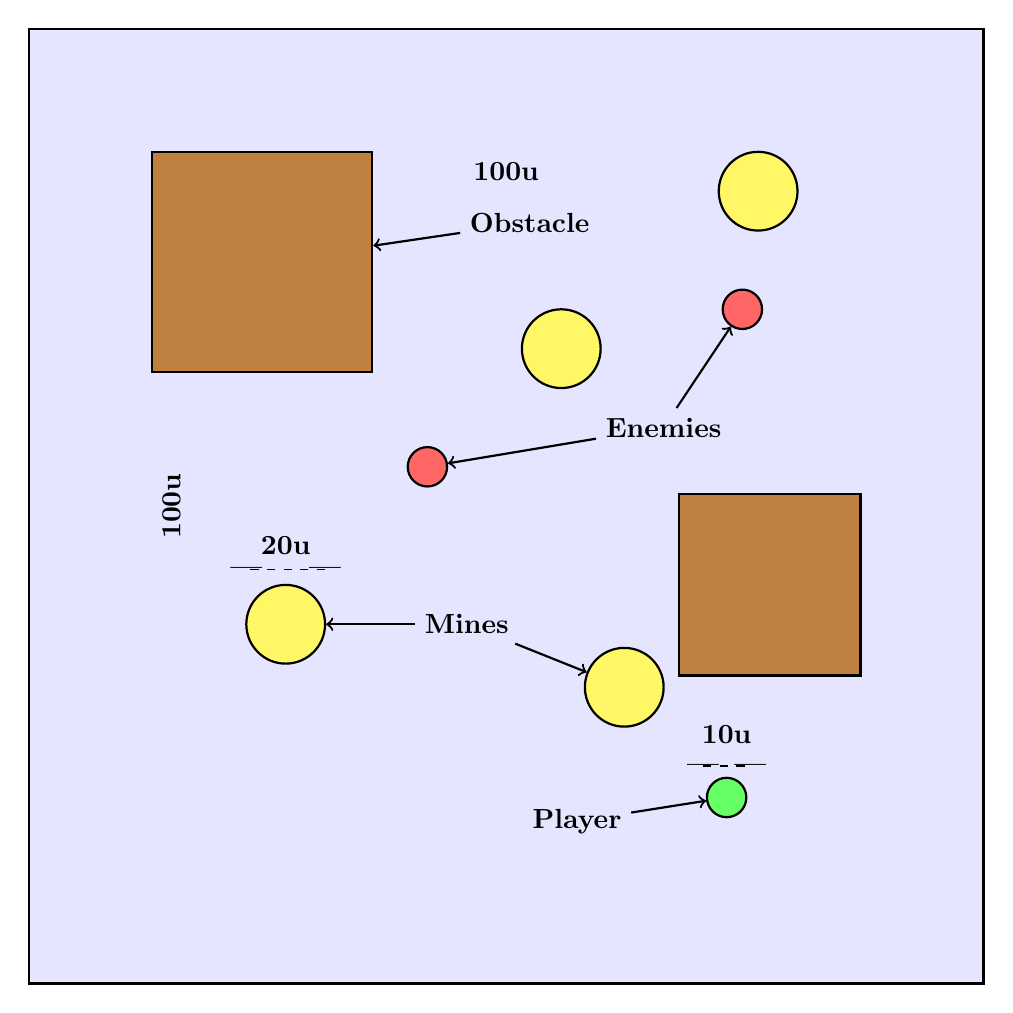
\begin{tikzpicture}[]
	\tikzstyle{sub}=[thick, draw, circle, align=center, minimum size = 0.5cm]					
	\tikzstyle{mine}=[thick, draw, circle, align=center, minimum size = 1cm, fill=yellow!60!white]					
	\tikzstyle{obstacle}=[thick, draw, rectangle, align=center, fill=brown]					
	\node[align=center, fill=blue!10!white, thick, draw, thick, rectangle, minimum height=\columnwidth, minimum width=\columnwidth](tarea)at (0,0) {};
	\node[](a1)at (0, 4.25) {\bf 100u};
	\node[rotate=90](a1)at (-4.25, 0) {\bf 100u};
	
	\node[obstacle, minimum size=2.8cm](obs1)at (-3.1, 3.1) {};
	\node[obstacle, minimum size=2.3cm](obs2)at (3.35, -1) {};
	\node[](tobs)at (0.3, 3.6) {\bf Obstacle};
	\draw[->, thick](tobs) -- (obs1);

	\node[fill=green!60!white, sub](player)at (2.8, -3.7) {};	
	\node[](tplayer)at (0.9, -4) {\bf Player};
	\draw[->, thick](tplayer) -- (player);
	\node[](a1)at (3.1, -3.3) {\bf |};
	\node[](a2)at (2.5, -3.3) {\bf |};
	\draw[-, dashed](2.5, -3.3) -- (3.1, -3.3);
	\node[](a2)at (2.8, -2.9) {\bf10u};
	
	\node[fill=red!60!white, sub](enemy1)at (-1, 0.5) {};	
	\node[fill=red!60!white, sub](enemy2)at (3, 2.5) {};
	\node[](tenemy)at (2, 1) {\bf Enemies};
	\draw[->, thick](tenemy) -- (enemy1);
	\draw[->, thick](tenemy) -- (enemy2);
	
	\node[mine](mine1)at (-2.8, -1.5) {};	
	\node[mine](mine2)at (1.5, -2.3) {};
	\node[mine](mine3)at (0.7, 2) {};
	\node[mine](mine4)at (3.2, 4) {};
	\node[](tmines)at (-0.5, -1.5) {\bf Mines};
	\draw[->, thick](tmines) -- (mine1);
	\draw[->, thick](tmines) -- (mine2);
	
	\node[](a1)at (-3.3, -0.8) {\bf |};
	\node[](a2)at (-2.3, -0.8) {\bf |};
	\draw[-, dashed](-2.3, -0.8) -- (-3.3, -0.8);
	\node[](a2)at (-2.8, -0.5) {\bf20u};	
	\end{tikzpicture}
\end{figure}
%
\vfill
%
At the start of the game, spread the player and enemy submarines as well as possible obstacles on the map.
In addition, determine the positions of the mines, but keep them secret until they are stepped on or detected by the sonar.
Before the game starts, the players can choose one of 3 difficulty levels, which determines the amount mines and enemy submarines, as well as the prize received for winning.
%
\\\\
%
\oftable{p{0.2\columnwidth} p{0.35\columnwidth} p{0.4\columnwidth}}
{\accf{Difficulty} & \accf{Enemies / Mines} & \accf{Prize}}
{
	Easy 	& 1 / 2 & Dark Matter \ofrow
	Medium	& 2 / 4 & Wet Floor Materia \ofrow
	Hard 	& 3 / 6 & Gold Hairpin \ofrow
}
%
\clearpage
%
%
%
%
%
%
%
%
%
\includegraphics[width=\columnwidth]{./art/goldsaucer/chocoborace.jpg}
%
\vfill
%
\accf{Chocobo Racing} is a racing game with an entry fee of 2 GP per player.
Each player is a rider in the race and they can either choose one of the following Chocobos provided by the park or they can use a Chocobo that they own.
The GM adds and plays additional participants in the race until there are 5 competitors in total.
%
\\\\
%
\oftable{p{0.35\columnwidth} p{0.3\columnwidth} p{0.3\columnwidth}}
{\accf{Chocobo} & \accf{Stamina} & \accf{Agility}}
{
	Echo 	& 4 & 5 \ofrow
	Fives 	& 5 & 4 \ofrow
	Rex 	& 6 & 3 \ofrow
	Cody 	& 7 & 2 \ofrow
	Jesse   & 8 & 1 
}
%
\vfill
%
A race consists of multiple rounds and during a round, each participant performs a sprint check to determine which distance they can cover.
Participants continuously add up the results of all their checks as their total score and the first one to surpass 50 points wins the race.
The score of every participant should be announced at the end of each round to keep track of the current state of the race.
If multiple participants reach the finish line in the same round, the one with the highest score wins the race.
The sprint check performed on each turn is modified as follows:\ofrow
%
\ofbullet{%
	The result of each sprint check is reduced by the difference between the Chocobo's Stamina and its current fatigue. 
	Everyone starts with 0 fatigue and gains 1 fatigue at the end of each round.
	For example, if a Chocobo has a fatigue of 10 and a Stamina of 8, the result of their check would be reduced by 2, but if  it had 10 or more Stamina it would receive no penalty.
	This reduction cannot cause the result of a sprint to drop below 0.
}
\ofbullet{%
	Before each check, a participant can decide to perform a dash action.
	In this case, they gain Advantage on the sprint check, but also an additional point of fatigue.
	Within a race, you can dash only a maximum amount of times equal to the Chocobo's Agility.
}
\ofbullet{%
	Characters who are particularly good at handling Chocobos gain Advantage on all sprint checks.
}
%
\\\\
%
When the race is finished, the winner rolls 1d and receives a prize based on the result.
%
\newpage
%
\oftable{p{0.4\columnwidth} p{0.7\columnwidth}}
{\accf{Result} & \accf{Prize}}
{
	1 & 10 GP \ofrow
	2 & Phoenix Down \ofrow
	3 & Signal Materia \ofrow
	4 & Elixir \ofrow
	5 & Angel Materia \ofrow
	6 & Hermes Boots
}
%
\\\\
%
%
%
%
%
%
%
%
%
\begin{center} \includegraphics[width=\columnwidth]{./art/goldsaucer/snowgame.jpg} \end{center}
\accf{Snow Game} is a snowboarding game that costs 1 GP to play per player.
The game can be played by multiple players who race down a ski run trying to reach a high score.
This score starts at 0, collecting balloons increases it, while hitting obstacles reduces it, so the score can become negative.
The course has 3 lanes: left, center and right and the players start on the center lane, going down the ski run back to back.
The game plays out over 8 rounds and at the start of each round, the GM rolls 3d, one die after the other, to determine the objects on the 3 lanes in front of the players from left to right.
The table below shows the possible objects based on the die results and their effects that occur when a players collide with them.
%
\\\\
%
\oftable{p{0.3\columnwidth} p{0.35\columnwidth} p{0.3\columnwidth}}
{\accf{Result} & \accf{Object} & \accf{Effect}}
{
	1 - 2 & Nothing & -- \ofrow
	3 & Snowman & - 1 point\ofrow
	4 & Rock & - 2 points \ofrow
	5 & Red Balloons & + 1 point\ofrow
	6 & Blue Balloons & + 2 points \ofrow
}
%
\\\\
%\clearpage
%
After learning about the objects in front of them, each player can decide between 1 of 3 actions:\ofrow
\ofbullet{\accf{Move one lane to the left or right:} make a DC~6 check, if you succeed you successfully change one lane, otherwise you stay in your current one.} 
\ofbullet{\accf{Move two lanes to the left or right:} make a DC~8 check, if you succeed you successfully change two lanes, otherwise you stay in your current one.} 
\ofbullet{\accf{Jump:} make a DC~8 check. If you succeed, you avoid the object in front of you and you gain 1 point. If you fail, you collide with the object in front of you and you additionally lose 1 point. You can take this action even if there are not objects in front of you.} \ofrow
Characters with particularly good coordination or experience with snowboards gain Advantage on these checks.
After all actions have been taken, check which lane each player ends up in and whether they collide with any objects to adjust the scores accordingly before the next round starts.
At the end of the 8th round, all players reaches the finish line and depending on their score each player receives one of the following prices.
%
\\\\
%
\oftable{p{0.4\columnwidth} p{0.7\columnwidth}}
{\accf{Score} & \accf{Prize}}
{
	< 4 & Participation Trophy \ofrow
	4 - 5 & X-Potion \ofrow
	6 - 7 & Safety Bit \ofrow
	8 - 9 & HP Plus \ofrow
	> 9 & 50 GP \ofrow
}
%
%
\ofpar
%
%
%
%
%
%
\includegraphics[width=\columnwidth]{./art/goldsaucer/gbike.jpg}
\\\\
\accf{G-Bike} is a biking game where the players are chased by hostile bikers on a highway and have to fight them off to escape.
The game can be played by multiple players with an entry fee of 1 GP per player.
The highway has 4 lanes and the focus is always put on 3 rows, so there are 12 total positions where bikers and obstacles can be positioned at a given time.
The illustration below shows how the map might look like during the game.
%
%\newpage
%
\begin{figure}[h!]
	\centering
	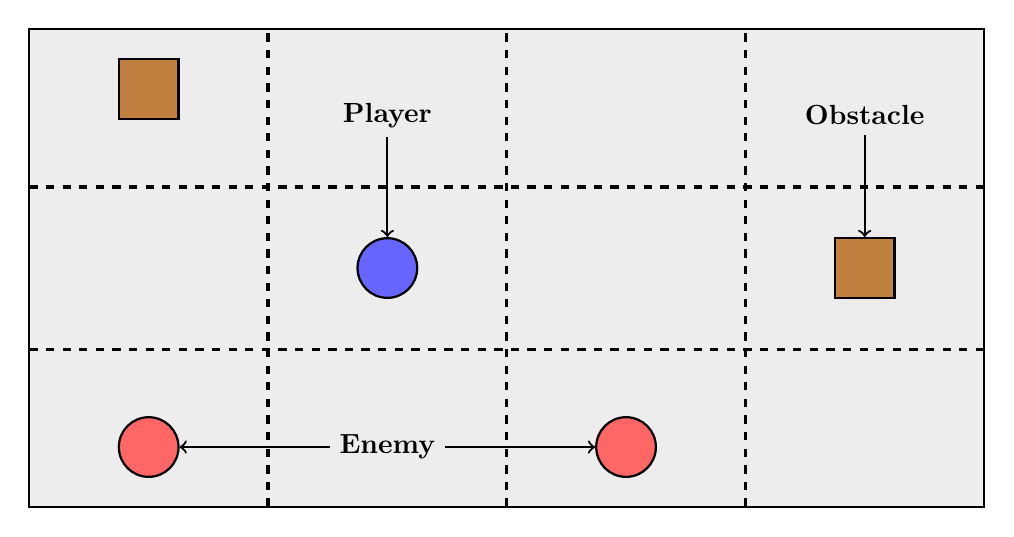
\begin{tikzpicture}[]
	\tikzstyle{biker}=[thick, draw, circle, align=center, minimum size = 0.5*0.125\columnwidth]					
	\tikzstyle{obstacle}=[thick, draw, rectangle, align=center, fill=brown, minimum size=0.5*0.125\columnwidth]					
	
	\node[align=center, thick, draw, thick, rectangle, minimum height=0.5\columnwidth, minimum width=\columnwidth, fill=black!7!white](tarea)at (0,0) {};		
	\draw[very thick, -, dashed](-0.25\columnwidth, -0.25\columnwidth) -- (-0.25\columnwidth, 0.25\columnwidth);
	\draw[very thick, -, dashed](0, -0.25\columnwidth) -- (0, 0.25\columnwidth);
	\draw[very thick, -, dashed](0.25\columnwidth, -0.25\columnwidth) -- (0.25\columnwidth, 0.25\columnwidth);
	\draw[very thick, -, dashed](-0.5\columnwidth, 0.5*-0.17\columnwidth) -- (0.5\columnwidth, 0.5*-0.17\columnwidth);
	\draw[very thick, -, dashed](-0.5\columnwidth, 0.5*0.17\columnwidth) -- (0.5\columnwidth, 0.5*0.17\columnwidth);
	
	\node[fill=red!60!white, biker](b1)at (-0.375\columnwidth, 0.5*-0.375\columnwidth) {};
	\node[fill=red!60!white, biker](b2)at (0.125\columnwidth, 0.5*-0.375\columnwidth) {};
	\node[fill=blue!60!white, biker](b3)at (-0.125\columnwidth, 0) {};
	\node[obstacle](obs1)at (0.375\columnwidth, 0) {};
	\node[obstacle](obs2)at (-0.375\columnwidth, 0.5*0.375\columnwidth) {};
	
	\node[](tobs)at (0.375\columnwidth, 0.16\columnwidth) {\bf Obstacle};
	\draw[->, thick](tobs) -- (obs1);
	\node[](tplayer)at (-0.125\columnwidth, 0.16\columnwidth) {\bf Player};
	\draw[->, thick](tplayer) -- (b3);
	\node[](tenemy)at (-0.125\columnwidth, 0.5*-0.375\columnwidth) {\bf Enemy};
	\draw[->, thick](tenemy) -- (b1);
	\draw[->, thick](tenemy) -- (b2);
	\end{tikzpicture}
\end{figure}
%
\newpage
%
The game plays out over 8 rounds and during each round, first all players take one turn and then all hostile bikers.
Player bikers start with 3 HP and enemy bikers start with 1 HP, when a biker is reduced to 0 HP, he is removed from the game.
During a turn, each biker may make a movement and take one Attack action:
\vfill
\ofbullet{\accf{Movement:} move either one lane to the left / right or one row to the front / back if that position is not occupied by an obstacle or another biker. Alternatively, you can try to activate the bike turbo. In this case, make a DC~8 check, if you succeed you can make two movements on this turn, if you fail, you cannot move at all. Characters with particularly good vehicle handling receive Advantage on this check}\ofpar
\ofbullet{\accf{Melee Attack:} make a DC~6 check. If you succeed, a biker who is 1 movement away from you suffers 1 HP damage.}\ofpar
\ofbullet{\accf{Ranged Attack:} make a DC~8 check. If you succeed, a biker who is 2 or less movements away from you, suffers 1 HP damage.}
%
\vfill
%
At the start of each round, roll 1d for every player that is still in the game.
Based on the results, place the following items in any open position of your choice: 1-2:nothing, 3:red biker,  4:blue biker, 5-6:obstacle.
However, do not place any more hostile bikers if there are already as many of them in the game as players.
Red and blue bikers are controlled by the GM and follow the same rules as players, but red bikers can only perform ranged attacks while blue bikers can only perform melee attacks.
Obstacles all follow the same rules and the GM is free to choose their appearance, they could for example be roadblocks or other vehicles.
Whenever a player biker ends his turn with an obstacle in the same lane in front of him, he has to make a DC~8 check, if he succeeds he jumps over the obstacle and if not, he suffers 1 HP damage.
Enemy bikers evade all obstacles automatically.
At the end of each round, all bikers stay in their positions and all obstacles disappear as they are left behind the current field of focus.
Every player biker who survives until the end of the 8th round wins a prize.
Each winner rolls 1d and depending on the result, he receives one of the following prizes.
%
\vfill
%
\oftable{p{0.4\columnwidth} p{0.5\columnwidth}}
{\accf{Result} & \accf{Prize}}
{
	1 	 & Item Holder \ofrow
	2    & 5 GP \ofrow		
	3    & Turbo Ether \ofrow
	4    & Phoenix Down \ofrow
	5    & Alert Materia \ofrow    
	6    & Bomb Materia
}
%
\clearpage
%
%
%
%
%
\includegraphics[width=\columnwidth]{./art/goldsaucer/proxycatcher.jpg}
%
\vfill
%
\accf{Proxy Catcher} is a crane game that costs 4 GP to play.
The game is played by a single player who uses the controls of the machine to navigate a crane and potentially pick a valuable prize from a pile.
The player only has one chance to lower the crane and grab something.
To do so, the player makes a check and receives a prize based on the result as listed in the table below.
However, the game is rigged as the crane has a fixed chance of properly grabbing something.
Players can perform a DC~8 check to understand that the player skill has barely any influence on the odds of success.
%
\vfill
%
\oftable{p{0.5\columnwidth} p{0.5\columnwidth}}
{\accf{Result} & \accf{Prize}}
{
	2 - 5 & Nothing \ofrow
	6 - 7 & Potion \ofrow
	8     & 5 GP \ofrow		
	9     & Ether \ofrow
	10    & Phoenix Down \ofrow
	11    & 20 GP \ofrow    
	12    & Counter Materia
}
\vfill
%
{
\begin{center}\includegraphics[width=0.7\columnwidth]{./art/goldsaucer/caitsith.jpg}\end{center}
%
%
%
%
\newpage
%
\includegraphics[width=\columnwidth]{./art/goldsaucer/arena.jpg}
%
\vfill
%
The \accf{Colosseum} is a battle arena that costs 1 GP per player to participate in.
All players that want to participate, fight up to 7 groups of monsters together as a party, one after another, on a 10u by 10u battlefield with walls on all 4 sides.
After the party defeats one group, roll 1d and depending on the result, they receive an additional handicap in each subsequent fight.
If you roll the same number twice, roll again until you get a handicap that is not active yet.
The list below shows the 6 possible handicaps, so by time the party reaches the 7th round, all of them will be active.
%
\vfill
%
\oftable{p{0.15\columnwidth} p{0.75\columnwidth}}
{\accf{Result} & \accf{Handicap}}
{
	1 & You can no longer equip Materia. \ofrow
	2 & You can no longer use Items.  \ofrow
	3 & You can no longer equip Accessories. \ofrow
	4 & You can no longer equip Armor.  \ofrow
	5 & You can no longer use Limit Breaks. \ofrow
	6 & You suffer Zombie until you leave the Colosseum (cannot be removed). \ofrow
}
%
\vfill
%
After defeating a group, everyone in the party can take an additional turn before the next fight starts.
At that point, they can also decide to forfeit and collect a prize depending on how many rounds they have completed.
If the entire party is defeated within a round, they do not receive any prize.
In any case, the party fully recovers their HP and MP after leaving the Colosseum.  
The list below shows the possible prizes depending on how many rounds were completed.
The following page shows the 7 types of monsters encountered from the 1st to the 7th round.
At the start of each round, place as many of the current round's monster type on the battlefield as there are players.
%
\vfill
%
\oftable{p{0.4\columnwidth} p{0.75\columnwidth}}
{\accf{Round} & \accf{Prize}}
{
	1 & Potion \ofrow
	2 & Phoenix Down \ofrow
	3 & 10 GP \ofrow
	4 & Lure Materia  \ofrow
	5 & Blaze Materia \ofrow
	6 & Protect Bangle \ofrow
	7 & Genji Gloves \ofrow
}
%
\clearpage
%
\ofmonster{Python (Round 1)}{3}{\includegraphics[width=0.2\columnwidth]{./art/goldsaucer/python.jpg}}
{
	HP: & \hfill 24 & MP: & \hfill 18\\
	STR: & \hfill 3 & DEF: & \hfill 1 \\
	MAG: & \hfill 0 & RES: & \hfill 3 \\
	AGI: & \hfill 3 & Size: & \hfill M\\
}
{\accf{Bite}: 1d DMG \hfill \accf{Immune:}\poison \hfill \accf{Weak:}\earth}
{	
	\mtech{Entangle}{6}{0r}{Single}{3u}{The target makes a DC 8 check and suffers 2d damage and Immobile for 1 round upon failure.}{\immobile}		
}
%
\vfill
%
\ofmonster{Hecteyes (Round 2)}{4}{\includegraphics[width=0.2\columnwidth]{./art/goldsaucer/hecteyes.jpg}}
{
	HP: & \hfill 32 & MP: & \hfill 50\\
	STR: & \hfill 1 & DEF: & \hfill 2 \\
	MAG: & \hfill 6 & RES: & \hfill 8 \\
	AGI: & \hfill 2 & Size: & \hfill M\\
}
{\accf{Tackle}: 2d DMG \hfill \accf{Immune:}\sleep \hfill \accf{Weak:}\lightning}
{	
	\mspell{Blind}{6}{1r}{Single}{3u}{The target makes a DC 8 check and suffers Blind for 3 round upon failure.}{\blind}		
	\mspell{Thunder}{4}{1r}{Single}{3u}{You deal 2d lightning damage to the target.}{\ice}		
}
%
\vfill
%
\ofmonster{Mantis (Round 3)}{5}{\includegraphics[width=0.23\columnwidth]{./art/goldsaucer/mantis.jpg}}
{
	HP: & \hfill 46 & MP: & \hfill 30\\
	STR: & \hfill 4 & DEF: & \hfill 2 \\
	MAG: & \hfill 0 & RES: & \hfill 2 \\
	AGI: & \hfill 3 & Size: & \hfill M\\
}
{\accf{Cut}: 2d DMG \hfill \accf{Immune:}\immobile \hfill \accf{Weak:}\fire}
{	
	\mtech{Metal Cutter}{4}{0r}{Single}{Weapon}{Make an Attack against the target. If you succeed, the damage dealt ignores the target's DEF.}{}		
	\mpassive{Leap}{When moving you can jump over enemies and obstacles up to a height of 2u, instead of having to walk around them.}	
}
%
\vfill
%
\ofmonster{Griffon (Round 4)}{6}{\includegraphics[width=0.23\columnwidth]{./art/goldsaucer/griffon.jpg}}
{
	HP: & \hfill 67 & MP: & \hfill 50\\
	STR: & \hfill 6 & DEF: & \hfill 3 \\
	MAG: & \hfill 0 & RES: & \hfill 5 \\
	AGI: & \hfill 3 & Size: & \hfill M\\
}
{\accf{Claw}: 2d DMG \hfill \accf{Immune:}\immobile\blind \hfill \accf{Resilient:}\wind}
{	
	\mtech{Feather Shot}{6}{0r}{Single}{4u}{The target suffers 3d wind damage.}{\wind}		
	\mpassive{Peck}{Whenever you successfully Attack a target he makes a DC 7 check and suffers Blind for 3 rounds upon failure.}
}
%
\newpage
%
\ofmonster{Big Horn (Round 5)}{7}{\includegraphics[width=0.23\columnwidth]{./art/goldsaucer/bighorn.jpg}}
{
	HP: & \hfill 90 & MP: & \hfill 80\\
	STR: & \hfill 7 & DEF: & \hfill 5 \\
	MAG: & \hfill 0 & RES: & \hfill 5 \\
	AGI: & \hfill 2 & Size: & \hfill L\\
}
{\accf{Tackle}: 3d DMG \hfill \accf{Immune:}\poison \hfill \accf{Resilient:}\fire}
{	
	\mtech{Charge}{8}{1r}{Single}{10u}{Dash towards the target and deal 3d damage to him. In addition, the target is knocked back by 3u and if he hits a wall, he suffers an additional 3d damage.}{}		
	\mreaction{Kickback}{Whenever you suffer damage from an enemy within 1u, you can deal 10 physical damage to him and knock him back by 2u.}
}
%
\vfill
%
\ofmonster{Golem (Round 6)}{8}{\includegraphics[width=0.23\columnwidth]{./art/goldsaucer/golem.jpg}}
{
	HP: & \hfill 130 & MP: & \hfill 100\\
	STR: & \hfill 9 & DEF: & \hfill 8 \\
	MAG: & \hfill 0 & RES: & \hfill 6 \\
	AGI: & \hfill 2 & Size: & \hfill L\\
}
{\accf{Fist}: 3d DMG \hfill \accf{Immune:}\poison\sleep\ \hfill \accf{Resilient:}\earth}
{	
	\mspell{Quake}{20}{1r}{3u}{7u}{Deal 6d earth damage to everyone in the target area.}{\earth}
	\mtech{Earth Wall}{12}{0r}{3u (line)}{3u}{You create a 3u tall and wide wall of earth that blocks the path. The wall breaks down after 3 rounds or upon suffering a total of 15 damage.}{}
}
%
\vfill
%
\ofmonster{Dark Dragon (Rnd 7)}{9}{\includegraphics[width=0.24\columnwidth]{./art/goldsaucer/blackdragon.jpg}}
{
	HP: & \hfill 200 & MP: & \hfill 180 \\
	STR: & \hfill 10 & DEF: & \hfill 7 \\
	MAG: & \hfill 9 & RES: & \hfill 8 \\
	AGI: & \hfill 3 & Size: & \hfill L\\
}
{\accf{Bite}: 3d DMG \hfill \accf{Resilient}:\fire\ice\dark \\ \accf{Immune}: All Status Effects}
{
	\mtech{Obliterating Breath}{16}{0r}{3u (front)}{3u}{Everyone in the target area makes a DC 8 check and suffers 4d damage as well as Poison and Blind for 3 rounds upon failure.}{\poison \blind}{}
	\mspell{Dark Flare}{30}{2r}{Single}{5u}{You deal 6d+20 dark damage to the target.}{\dark}
	\mpassive{Tail Whip}{Whenever you Attack, you can choose to target all enemies within 1u at once.}	
}	
%
\clearpage
\ofsubsection{Maria \& Draco}
%
\ofquote{"The West and East were waging war.
Draco, the West's great hero, thinks of his love, Maria.
Is she safe? Is she waiting?
The forces of the West fell, and Maria's castle was taken.
Prince Ralse, of the East, took her hand by force. But she never stopped 
yearning for Draco..."\\}{Excerpt from opera "Maria \& Draco"}
%
\vfill
%
\includegraphics[width=\columnwidth]{./art/mariaanddraco/opera.jpg}
%
\vfill
%
\accf{Maria \& Draco} is a prepared adventure that can be completed in a single session and is designed for a party of Level~3 characters.
Their stories of the protagonists should explain why they are presently staying at the wealthy city Jidoor.
In this adventure, the party is tasked with preventing the kidnapping of a famous opera singer.
%
\vfill
%
\ofquote{"This is simply horrid! I want the performance to be a success! But I don't want Maria to be abducted!"\\}{Impresario}
%
\vfill
%
While resting at the city of Jidoor, the adventurers meet the owner of the town's opera house, he calls himself "Impresario".
He is an older, well-dressed man who is in constant worry about the upcoming opera called "Maria \& Draco".
Impresario is desperately looking for security guards for tomorrow's opera performance.
He offers 1000G to the party for handling the job, which they accept, despite not being paid up front.
At the morning of the opera, they meet Impresario at the opera house.
As they enter, he is running around frantically and upon noticing the party, he immediately hands them the following letter.\\
%
\vfill
%
Dearest Maria,\vspace{0.6cm}\\
I have decided to take you as my wife, so I'll be coming to kidnap you.\vspace{0.6cm}\\
\hspace*{0.5cm}The Wandering Gambler\\
%
\newpage
%
After he has calmed down, Impresario explains that the "Wandering Gambler" is a man named Setzer Gabbiani, who has caused trouble to him in the past.
He further describes Setzer as "a gambling vagabond who finds freedom from society's narrow views of morality aboard his airship" in a sarcastic tone.
Impresario also explains that Maria is the star of the show, so her safety is of utmost importance.
He proposes the following plan to keep her safe: one of the party members should play the role of Maria and act as a decoy.
He expects Setzer to make his move at the end of the first scene and try to abduct Maria onto his airship, but if he kidnaps the decoy, they can confront him instead.
He suggests that the decoy should carry a rope, so he or she can pull up the rest of party onto the airship if necessary.
The party may suggest other ideas as well, but Impresario will not accept any plan that might put the real Maria in danger.
If the party accepts his plans, they have to choose one of their own to play Maria's part in the opera, henceforth that character will be referred to as "Maria".
%
\vfill
%
\ofquote{"W...wait! I'm a GENERAL, not some opera floozy!"\\}{Celes}\\\\
%
Impresario will show them Maria's room, where "Maria" can get dressed and practice for her part.
"Maria" has to look as similar to the original as possible, who is a short, blond haired women in a long white dress.
Accordingly, the party might have to buy a new dress and wig or get creative in other ways, they can convince Impresario to cover additional costs. 
They are free to explore the town to shop or make other preparations until the evening. 
"Maria" should practice the following script for her part in the first scene:
%
\vfill
%
Maria enters the stage.\vspace{0.2cm}\\
"Oh my hero, so far away now. Will I ever see your smile?"\vspace{0.2cm}\\ 
"Love goes away, like night into day. It's just a fading dream."\vspace{0.2cm}\\ 
"Our love is brighter than the sun. For eternity, for me there can be, only you, my chosen one."\vspace{0.2cm}\\ 
Maria picks up the flowers, climbs the stairs to the balcony high atop the castle, then raises the flowers to the stars.\vspace{0.2cm}\\
"We must part now. My life goes on. But my heart won't give you up."
%
%
\vfill
%
During the opera, "Maria" first appears at the end of the first scene, where she has to perform the above mentioned part.
You as the GM have to rate "Maria's" performance on a scale from 1 to 10.
Below is a list of criteria, which you can use to award points.
You should keep the rating secret at this point, but you can to already give a hint by narrating the reaction of the audience.
%
\clearpage
%
\includegraphics[width=\columnwidth]{./art/mariaanddraco/maria.jpg}\\
%
\vfill
%
\ofbullet{1 point for each line that the player correctly recites, so up to 4 points.}
\ofbullet{1 bonus point, if the player makes an attempt to actually sing the lines.}
\ofbullet{Up to 3 points depending on how much effort the party has spent on making "Maria" actually look like Maria.}
\ofbullet{1 point if the player remembers to pick up the flowers, walk up the stairs and raise the flowers up.}
\ofbullet{The player makes a DC~8 to determine whether his or her character manages to present themselves as gracefully as the real Maria. If the check succeeds, award another 2 points. The DC can be lower if "Maria" has any performance related experience.}
%
\vfill
%
\includegraphics[width=\columnwidth]{./art/mariaanddraco/ultros.jpg}
%
\vfill
%
As Maria's part is playing out on the stage, Impresario and the party are watching from their lodge seats.
Suddenly, Impresario notices something on the catwalk: someone, or rather something, is trying to push an anvil down onto the stage!
The party recognizes that it is the strange octopus named Ultros who is behind the plan.
The adventurers have met Ultros before and have beaten him, so he wants to take revenge by sabotaging the opera. 
Impresario starts to panic and begs the party to stop Ultros's plan.
He points them to a room on the right hand side of the lodge and tells them to pull the rightmost lever.
%
\newpage
%
\ofquote{"Silence! You are in the presence of octopus royalty! A lowborn thug like you could never defeat me!"\\}{Ultros}\\\\
%
After they move out of their seats, each party member has to make a DC~6 check to decide whether they disturb the audience.
If at least one of them fails, deduct one point from the performance.
Once in the room, the party notices four levers on the wall.
The rightmost lever opens a pathway to the catwalk, the other ones have the following effects and pulling either one deducts a point from Maria's performance: lever 1 makes a sound like a barking dog, lever 2 turns off the lights in the opera hall and lever 3 opens up a trap door below the player who pulled the lever, which lets him or her slide directly onto the stage. 
Once the party enters the catwalk, they see that Ultros is just about to drop the anvil on "Maria".
As they move closer, the fragile planks of the catwalk fail to support their combined weight and both the party and Ultros
fall down onto the stage.
"Maria" has to make a DC~7 check and if she fails, she falls unconscious, otherwise she can participate in the ensuing battle.   
The ones who fell, including Ultros, take 1d damage, but they can immediately get up to start the fight!
%
\vfill
%
\ofmonster{Ultros}{3}{\includegraphics[width=0.32\columnwidth]{./art/mariaanddraco/ultrosmon.jpg}}
{
	HP: & \hfill 60 & MP: & \hfill 90 \\
	STR: & \hfill 4 & DEF: & \hfill 2 \\
	MAG: & \hfill 1 & RES: & \hfill 3 \\
	AGI: & \hfill 2 & Size: & \hfill L\\
}
{\accf{Ink}: 1d DMG, 3u Range \hfill \accf{Drops:} 500G\\
\accf{Immune}:\poison\sleep\blind\immobile \hfill \accf{Final Attack, Dual Attack}
}
{	
	\mspell{Water}{6}{0r}{Single}{4u}{You deal 2d water damage to the target.}{\water}
	\mtech{Acid Rain}{8}{0r}{3u}{Self}{
		All enemies in the target area suffer 2d water damage.
		In addition, all affected targets make a DC~7 check and suffer Poison for 1 round upon failure 
	}{\poison\water}	
	\mtech{Tentacle}{4}{0r}{2u (front)}{Self}{Deal 2d damage to all enemies in the target area.}{}	
	\mpassive{Blindtouch}{Every target that rolls below 6 on an evasion check against your Attack, suffers Blind for 3 rounds.}{}		
}
%
\vfill
%
After the party defeats Ultros, they hear a voice loudly exclaiming: "What a performance!".
Suddenly, a man descends onto the stage using a grappling hook.
The man is of course none other than Setzer.
He quickly grabs "Maria" and activates the device once more to pull himself back up to the lodge with "Maria" in his arms.
From there he escapes to his airship, which is waiting right above the rooftop of the opera house.
The party tries to follow him but they have to take a longer route to reach the the roof.
As they arrive at the rooftop, Setzer is just getting ready to take off with the airship.
%
\clearpage
%
\ofquote{"Nothing to lose but my life..."\\}{Setzer}\ofpar
%
%
\includegraphics[width=\columnwidth]{./art/mariaanddraco/setzer.jpg} 
%
\\\\
%
He locks "Maria" in his cabin and gets on deck to start the engine.
If "Maria" fell unconscious before, she will now wake up and realize that Setzer has abducted her.
If everything went according to plan up to this point, she should have a rope with her.
She can let it out of one of the windows in this room and the party can reach from the roof. 
Optionally, you can ask each player to perform a DC~7 check to decide whether they are able to successfully grab and climb the rope.
After gaining some distance on the opera house, Setzer returns to the cabin.
Upon taking a closer look at "Maria" and noticing the rest of the party, he understands that he has been tricked and becomes angry.
The course of this confrontation depends on the decisions the party makes.
Below are some general ideas on roleplaying as Setzer, but you can, or might have to, improvise some aspects of this section.
%
\ofpar
%
\accf{The party tries to solve the conflict peacefully:}\\
Setzer is generally open to this as he realizes that he is outnumbered.
He can be convinced to let the party go and to stay away from the opera house in the future.
He is also open to joining the party, if they offer him the prospect of exciting future adventures.
Setzer is much easier to convince if the arrangement involves gambling of any sort, which he loves.
If the party tries to trick him, for example with a rigged coin toss, he will show even more respect.
However, he does not accept any deal that involves him being restrained or handed over to the authorities.
%
\ofpar
%
\accf{The party tries to kill or restrain Setzer forcefully:}\\
For this case, Setzer's combat statistics are listed below.
Despite being outnumbered, he does not give up easily and does not hesitate to use dirty tricks to get the upper hand.
If the party manages to defeat Setzer, they can decide whether they want to let him live or restrain him to deliver to the authorities.
Either way, they will need to maneuver and land the airship.
The player that takes control of the airship has to perform a check with a DC that can vary between 6 and 8, depending on the character's proficiency in handling vehicles.
If he or she fails the check, the ship crashes near Jidoor and gets destroyed.
All passengers on board survive, but everyone suffers 2d damage.
%
\vfill
%
\ofmonster{Setzer}{4}{\includegraphics[width=0.25\columnwidth]{./art/mariaanddraco/setzermon.jpg}}
{
	HP: & \hfill 40 & MP: & \hfill 80 \\
	STR: & \hfill 2 & DEF: & \hfill 1 \\
	MAG: & \hfill 0 & RES: & \hfill 1 \\
	AGI: & \hfill 4 & Size: & \hfill M\\
}
{
\accf{Cards}: 2d DMG, 3u Range \hfill \accf{Auto-Haste}
}
{
	\mtech{Slots}{8}{0r}{?}{?}{
		Roll 1d. One of the following effects occurs depending on the result:
		On a 1 or 2, the area within 3u of you is filled with smoke until the start of your next turn. 
		Everyone inside it, suffers Blind, but gains Blink.
		On a 3 or 4, you teleport to a location of your choice within 3u.
		On a 5 or 6, an explosion deals 2d fire damage to all enemies within 2u.
	}{}	
	\mtech{Gil Toss}{4}{0r}{2u}{5u}{You throw 100G to deal 2d damage to all enemies in the target area.}{}
	\mtech{Vanish}{8}{0r}{Single}{Weapon}{You become invisible for up to 5 rounds or until you take an action. While invisible, you gain Blink. Also, if you hit an Attack while invisible, you automatically score a Critical Hit.}{\blink}	
	\mreaction{Fixed Dice}{Whenever you roll for a check or to determine damage, you can re-roll one die that has the result~1.}{}		
}
%
\vfill
%
After dealing with Setzer, the party can return to the opera house to collect their reward.
Impresario considers their contract fulfilled if they have managed to drive away Setzer.
First, every party member gains a \accf{Level Up}!
In addition, they receive a reward depending on the rating of Maria's performance:\\\\
\ofbullet{\accf{1-3 points:} despite driving away Setzer, the opera performance was a disaster, leaving the audience deeply unsatisfied. Impresario blames the party for being sloppy and halves his originally offered reward to 500G.}\\\\
\ofbullet{\accf{4-6 points:} despite some hick ups, the performance went well overall. Impresario is satisfied and hands the party 1000G as agreed upon.}\\\\
\ofbullet{\accf{7-10 points:} the party managed to amaze the audience with an outstanding performance. Impresario is thrilled and doubles the originally agreed reward to 2000G.}
%
\clearpage
\ofsubsection{Siege of Dollet}
%
\ofquote{"The pride of Balamb Garden! The elite mercenary force, SeeD! Learn from them, obey their commands and accomplish the mission. Prove yourselves worth of
becoming a member of SeeD. Best of luck."}{Headmaster Cid}
%
\vfill
%
\includegraphics[width=\columnwidth]{./art/siegeofdollet/island.jpg}
%
\vfill
%
\accf{Siege of Dollet} is a prepared adventure that can be completed in a single session and is designed for a party of Level~2 characters.
The players take the role of students who are training to become members of an elite mercenary group called SeeD.
You as the GM take the role of their instructor to guide the students through their final exam.
%
\vfill
%
\ofquote{"Sounds boring. So what you're saying is, we do all the little, dirtywork..."}{Seifer}
%
\vfill
%
Good morning, instructor.
My name is Xu and I will provide you with as much intel throughout the day as I can.
You and all of your students that will be taking today's exam should currently be on one of our assault gunboats that are on the way to Dollet.
Remember, your job is only to guide the students, we want to see if they can prove themselves worthy of becoming SeeD.
As such, you will stay on this boat during the mission, but you can talk to the students at any time using the earpiece through which you are also hearing me right now.
Make sure that everyone makes it out alive!
%
\vfill
%
Concerning the mission:
the SeeD squads have been hired by the Dollet Parliament to defend them against a siege from the Galbadian army.
Your students form squad B and are tasked with clearing out and holding the inner city of Dollet.
We have intel that the majority of the Galbadian army have moved elsewhere, where the rest of the SeeD will be ambushing them. 
Make sure to go over these mission details with the students before you arrive. 
Oh, and don't forget to name one of them as the squad leader.
%
\newpage
%
\ofquote{"Look out, it's SeeD!"\\}{Galbadian Soldier}
%
\vfill
%
\includegraphics[width=\columnwidth]{./art/siegeofdollet/dollet.jpg} 
%
\vfill
%
You should soon arrive at Lapin Beach before Dollet.
The Galbadians have built up some defenses at the shore, but those should be no match for our gun boats.
After the beach is clear, squad B should leave the boat to start the exam.
They can move up the stairs to their left and from there follow the alley into the town square.
I can see 3 Galbadian soldiers guarding the town center, it could be more though.
Each student that passes a DC~7 check should be able to notice them as well.
Let's see how they handle themselves.
%
\vfill
%
\ofmonster{Galbadian Soldier}{2}{\includegraphics[width=0.15\columnwidth]{./art/siegeofdollet/gsoldier.jpg}}
{
	HP: & \hfill 13 & MP: & \hfill 0\\
	STR: & \hfill 2 & DEF: & \hfill 1 \\
	MAG: & \hfill 0 & RES: & \hfill 0 \\
	AGI: & \hfill 2 & Size: & \hfill M\\
}
{\accf{Machine Gun}: 1d DMG, 3u range \hfill \accf{Drops:} 200G}{}
%
\vfill
%
The Galbadians sure aren't making it easy for them.
They are using the fountain as a cover to avoid going into melee.  
After defeating these soldiers, squad B just needs to make sure that the inner city stays clear. 
If they decide to look around they might find some useful things like Potions.
There is also a lone dog wandering around, poor guy probably got lost in this mess.
It has been an hour now and I think the students are getting bored. 
Looks like everything is... wait a second.
I can see a large group of Galbadians moving quickly towards the town square!
Squad B needs to hide immediately! 
Hmm... it doesn't look like the soldiers want to retake the inner city, they are going somewhere else.
What are they up to?
%
\vfill
%
They are moving towards the mountain path, but there is nothing up there, except that old radio tower I think.
I don't know if the students understood what is going on, but the dog sure has.
Well at least he is howling at the mountain.
What are your orders instructor?
Remember, squad B needs to hold the inner city, but those Galbadians are clearly up to something.
I hope the students will follow your orders...
%
\clearpage
%
\ofquote{"WEDGE! Where were you!? No pay for you this month!"}{Major Biggs}
%
\vfill
%
\includegraphics[width=\columnwidth]{./art/siegeofdollet/tower.jpg}
%
\vfill
%
Squad B is also making its way up the mountain, I hope they make sure to stay undetected.
There are a few of Dollet's soldiers stationed on the path, but the Galbadians are cutting through them like butter.
Still, they are suffering many casualties on the way, I think only 2 Galbadians have actually made it to the tower.
Squad~B should be able to reach the tower without any issues.
Looks like they have almost reached the mountain top.
The Galbadians have meanwhile made their way up to the platform of the radio tower and I think they are making repairs.
At least they have managed to reactivate the radio tower.
That also means the students can take the elevator on the ground floor to reach them.
%
\vfill
%
\ofmonster{Major Biggs}{2}{\includegraphics[width=0.22\columnwidth]{./art/siegeofdollet/biggs.jpg}}
{
	HP: & \hfill 28 & MP: & \hfill 24\\
	STR: & \hfill 2 & DEF: & \hfill 2 \\
	MAG: & \hfill 1 & RES: & \hfill 1 \\
	AGI: & \hfill 2 & Size: & \hfill M\\
}
{\accf{Machine Gun}: 1d DMG, 3u Range \hfill \accf{Drops:} 500G}
{
	\mspell{Thunder}{4}{0r}{Single}{3u}{You deal 2d lightning damage to the target.}{\lightning}	
	\mtech{Rush}{3}{0r}{Single}{Weapon}{Make an Attack against the target. If you hit, you push him back by 1u on top of the damage dealt.}{}	
}
%
\vfill
%
\ofmonster{Wedge}{2}{\includegraphics[width=0.15\columnwidth]{./art/siegeofdollet/gsoldier.jpg}}
{
	HP: & \hfill 22 & MP: & \hfill 16\\
	STR: & \hfill 2 & DEF: & \hfill 1 \\
	MAG: & \hfill 1 & RES: & \hfill 1 \\
	AGI: & \hfill 3 & Size: & \hfill M\\
}
{\accf{Sword}: 1d DMG \hfill \accf{Drops:} 300G}
{\mspell{Fire}{4}{0r}{Single}{3u}{You deal fire damage to the target.}{\fire}	}
%
\newpage
%
I can now see squad B on the top of the tower, confronting the 2 Galbadian soldiers, one of them seems to be their leader. 
I think I have understood their strategy: they are trying force the students to the edge of the platform to knock them off the tower.
Should that happen, I think the students should be able to hold onto something if they pass a DC 5 check and another squad member can then spend an action to pull them back up. 
Anyway, the Galbadians do not seem very competent otherwise.
And... Squad B was able to neutralize the enemy!
We have also just received an important order:
all squads are to retreat back to Lapin Beach immediately, our boats depart in half an hour.
Squads that do not make it to the shore in 30 minutes will get left behind!
I think squad~B can... wait, what the kupo is THAT?!\\\\
%
\vfill
%
\ofmonster{X-ATM092}{4}{\includegraphics[width=0.3\columnwidth]{./art/siegeofdollet/mech.jpg}}
{
	HP: & \hfill ??? & MP: & \hfill 80\\
	STR: & \hfill 2 & DEF: & \hfill 3 \\
	MAG: & \hfill 0 & RES: & \hfill 1 \\
	AGI: & \hfill 4 & Size: & \hfill L\\
}
{\accf{Claw}: 2d DMG, 2u Range}
{
	\mtech{Ray Bomb}{5}{0r}{2u}{5u}{You deal 2d fire damage to all enemies inside the target area.}{\fire}	
	\mtech{Arm Crush}{3}{0r}{Single}{Weapon}{The target makes a DC 8 check and suffers 2d damage and Immobile for 1 round upon failure}{\immobile}	
}
%
\vfill
%
I don't know where the Galbadians got that thing from, but it is running after the students.
It looks like the thing will overtake all squad members that fail to pass a DC 8 check, I hope the rest do not leave them behind.
There is no way squad B can destroy it in combat, especially if they want to make it in time.
But there is another way: if they attack its legs a few times, it will collapse and begin to repair itself, which gives them time to run.
It's one of the known common vulnerabilities in Galbadian machines, so it should work. 
Still, I think they will have to fight the thing at least twice before they reach the shore.
But maybe they can also come up with something to stop it, a blockade or distraction?
%
\vfill
%
Squad B is now running through Dollet and closing in on the beach, but the machine is still following them.
Instructor, there is a powerful machine gun mounted to the deck of your boat, it should melt through it! 
...I think you got it, great job! 
Squad B has also boarded the boat, so you are ready to go!
Phew... that was close, I hope everyone has made it out alive.
So what do you think Instructor, how did the students do on the exam?
Which ones should we promote to SeeD?
%
\clearpage
\ofsubsection{Ivalice Worldbook}
%
\ofquote{"Names don't matter. What's important is how you live your life."}{Ramza Belouve}\\\\
%
\includegraphics[width=\columnwidth]{./art/worldbook/everyone.jpg}
%
\ofrow
%
The \accf{Ivalice Worldbook} is a comprehensive document about the setting of the Final Fantasy Tactics video game.
It includes many details about its history and geography to help you create your own adventures in the same world.
This supplement is an updated version of the original version written by Bruno Carvalho, Paul (Papa Quackers) and Hywel Williams in 2017 which included rules for the Final Fantasy Role Playing Game 4th Edition~(\accf{FFPRG~4e}) system.
The content and ideas presented in this version of the worldbook are system agnostic and thus also applicable to other tabletop RPGs.
%
\ofpar
%
\accf{Final Fantasy Tactics}~(FFT) is a spin-off title in the main Final Fantasy series. 
Unlike most spin-offs, however, it has managed to be a great game on its own, having received universal acclaim upon its release, and critical opinion of the game has improved further over time. 
It is the first game of the Final Fantasy Tactics series and was released in Japan in June 1997 and in the United States in January 1998. 
The game combines thematic elements of the Final Fantasy video game series with a game engine and battle system unlike those previously seen in the franchise. 
In contrast to other 32-bit era Final Fantasy titles, Final Fantasy Tactics uses a 3D, isometric, rotatable playing field, with bitmap sprite characters.
For many Final Fantasy players, this represented their first foray into the Strategy RPG genre, with its own quirks and conventions established by several other games that came before, like Shining Force, the Langrisser series or Tactics Ogre. 
For this reason, and to celebrate the 20th anniversary of the original Japan release of this cult classic, this worldbook was born.
%
\vfill
%
Final Fantasy Tactics uses a three-dimensional isometric battle grid. 
This difference in functionality led to a game type that was more akin to chess than the traditional back and forth linear combat of previous Final Fantasy games. 
Instead of having six characters that were all-essential to the plot, and joined your party over a period, you had a singular main character that would occasionally be joined by story important characters that would depart and rejoin you when the plot demanded they do so. 
The bulk of your adventuring party was usually made up of interchangeable, nondescript characters whose appearance shifted radically depending on what \accf{job class} they were.
The progression of job classes in this system is quite similar to that of older Final Fantasy games, in that there were several job classes to choose from, but fundamentally different in how certain
job classes were unlocked. 
Instead of obtaining crystals that granted certain job classes automatically, you were given two starting job classes and expanded upon them. 
Your job progress reveals others, and if you took multiple levels in multiple jobs, your amalgamated experience in those two jobs might reveal another job class that was unique. 
This system involved a lot of job class switching and of course, a small amount of class mapping to determine which job classes unlocked another.
%
\vfill
%
\ofquote{"The best ways, don't always lead to the best results."\\}{Delita Hyral}\\\\
%
The story of Final Fantasy Tactics revolves around the aftermath of \accf{The 50 Year War}. 
The kingdom of \accf{Ivalice} is rife with political and economic discrepancies between the upper and lower class. 
This problem is compounded by the recent death of the king, whose only heir is an infant, and the need for a regent to rule in his place. 
The people are stuck between Prince Goltana, and Prince Large, known as the Black and White Lion respectively.
This leads into the main plot of the game, known as \accf{The Lion War}, in which you take on the role of \accf{Ramza Beoulve}. 
As the name implies, The Lion Wars were conflicts between the two princes in their attempt to become the ruling regent. 
Ramza is a young noble who takes part in many exploits of the war, discovers hidden corruption and machinations within the most powerful church in the lands, and comes to understand the plight of the common peoples. 
He was a decisive factor in the resolution of the war but was actively erased from history.
%
%
%
\clearpage
%
\ofsubsubsection{History}
%
\accf{The Beginning (10000 B.C. -- 2000 B.C.)}\\
During this period of time, estimated from 10000 to 2000 B.C. on the Ajorian Calendar, the majority of humankind lived on the southwestern coast of what years later would become Kaladis. 
Most of the people of these times were simply tribes of hunter-gatherers. 
As the age neared its close, however, metallurgy was developed as well as basic magic study. 
Unfortunately, there are extremely few records from this period, partly in thanks to a lack of a written language, which was first developed during the age of the Ronan Empire, although there are some rare ruins left behind that have been found in remote parts of Kaladis.
During this period, the countries that would later become Kaladis and Mizuno were first settled. Ivalice, Romanda, and Ordalia were first settled during the Ronan Empire.
%
\ofpar
\includegraphics[width=\columnwidth]{./art/worldbook/ovelia.jpg}
\ofpar
%
\accf{The Ronan Empire (2000 B.C. -- 700 B.C.)}\\
History dates the first true civilization as the Ronan Empire; an empire that grew from a humble farm village near Zeltenia to a huge empire that spanned most of what would become Ivalice and parts of Romanda and Ordalia near its end, roughly estimated between 700 and 600 B.C.. 
Not much is known about this mysterious empire save that it excelled at the use of magic even compared to the level used by the most powerful of today's magicians. 
Even more mysterious is what caused its downfall. 
The Ronan Palace, the center of the empire, was up until its discovery during the Lion Wars a myth in and of itself. 
Several important ruins originated from this era including Matoya's cave, the Tower of Babel, Mirage Tower, and of course the \accf{Ronan Palace}. 
The Ronan Empire was the first country to develop a written language with Mizuno soon following within its own language known as Nihonjin.
%
\ofpar
\includegraphics[width=\columnwidth]{./art/worldbook/tree.jpg}
\ofrow
%
\accf{The Age of Myth (700 B.C. -- 50 B.C.)}\\
Following the downfall of the Ronan Empire, the territories splintered into four separate countries: Melmond, the Baron Kingdom, the Kushuka Kingdom, and the Palamecian Empire. 
Like the Ronan Empire, these four nations covered Ivalice and began making inroads into the areas that would become Romanda and Ordalia in later years. 
This period is largely known as the age of myth in part due to the amount of fantastic ruins that were left behind as well as the level of technology developed.
\accf{Baron Kingdom} was a kingdom whose military might rivaled many of the other nations during the age of myth. 
Baron supported a large number of elite knights as well as a well-known navy of airships. 
Baron covered much of what would become Gallione, Fovoham, and western Lesalia.  
Compared to its neighbors, the \accf{Kushuka Kingdom} was a center of trade where traders from other countries would come to sell their wares. 
Unfortunately, for the country itself, its nobility ruled with harsh hand with little concern for their people.
After years of abusing the coffers of their nation, the royal family was dethroned by a huge revolution. 
On a modern map, Kushuka would occupy much of central Lesalia and most of Zeltenia.
Like its neighbors, the \accf{Palamecian Empire} had a specialty, namely technology. 
It was the first to develop airships and maintained a fleet that was a fair equivalent of Baron's navy. 
In addition to its airships, Palamecia also first developed guns that used magical ammunition as well as its "war golems", powerful robots that were used as first line soldiers and guards. 
The empire covered what would become Lionel. 
Many historians believe that its capital is deep below Goug Machine City. 
Palamecia was also the first to develop steam-powered devices and were the first to develop the science of magitek, which involves the fusing of magic and machine.
\accf{Melmond} was a secluded nation far to the east in what would later become southern Ordalia. 
More than other countries, Melmond embraced the study of magic in full and supported many academies dedicated to teaching the arcane arts to interested students. 
Other studies such as history, philosophy, and literature were also popular among Melmond people. 
Unfortunately, Melmond was considered by many of its neighboring countries to be working with the forces of Lucavi because of their magical might.
Like the Ronan Empire before them, all four kingdoms of the age of myth were destroyed by unknown circumstances. 
The \accf{Zodiac Brave Story} first emerged during this era. 
For those that do not know it, the Zodiac Brave Story is the tale of an evil king who called on the powers of Lucavi, around the year 500~B.C..
Lucavi killed the king and caused great havoc throughout the world. 
In the end, a small group of 12 heroes banded together and used the sacred zodiac stones to become the Zodiac Braves. 
The Zodiac Braves were able to defeat Lucavi and supposedly restored order. 
Following the defeat of Lucavi, the \accf{Holy Ydoran Empire} was founded, emerging from the ruins of the old Baron Kingdom.
The empire waged several wars, eventually defeating and conquering both Palamecia and Melmond.
%
\vfill
\includegraphics[width=\columnwidth]{./art/worldbook/delita2.jpg} 	
%
\newpage
%
\includegraphics[width=\columnwidth]{./art/worldbook/agrias.jpg}
\ofpar
%
\accf{The Life \& Death of St.~Ajora (50 B.C. -- 1 B.C.)}\\
The Ajorian Calendar begins its first year with the death of \accf{St.~Ajora} and the beginning of the \accf{Cataclysm}. 
By the time Ajora Glabados came, three of the four kingdoms of the age of myth had been conquered by the Holy Ydoran Empire, and the Kushuka Kingdom was the only other state to resist the power of its neighbor. 
The lands that once were Melmond laid abandoned and desolate, as refugees from the Jihads that would follow the rise of the Glabados Church would only resettle them several centuries later.
When Ajora Glabados was young, one day he sprang up, walked to a well, and prophesized that "soon, a calamity will befall this land. 
I am now sealing this well, and no one can drink from it." Several days later, the "Black Death" plagued Zeltenia. 
The people who drank from the contaminated well water fell ill and died one after another.
However, only the families that believed Saint Ajora's words survived and did not fall to disease. 
Since then, Saint Ajora became worshipped as "The Miracle Child" or "The Son of God".
Soon after these events, word of a new messiah spread, who would lead Ivalice out of the chaos born from years of war. 
By the time Ajora had reached 18 years old, he had already gained a devoted community of followers. 
Much like in earlier years, another ambitious king attempted to summon Lucavi. 
The emperor had created an army of immense size in the hopes of securing all of Ivalice under the Holy Ydoran Empire’s control. 
Once again, a new group of Zodiac Braves was created united by St.~Ajora to defeat the new Lucavi.
Despite his growing widespread fame, Ajora had made many enemies. 
The Holy Ydoran Empire feared Saint Ajora's rise to power; they feared his preaching of the coming of God. 
The \accf{Clergy of the Pharism} faith was the predominant religion and even though they had great influence, the clergy feared Saint Ajora's power. 
The conclusion is obvious.
Saint Ajora was captured with a secret tip from Germonik, Ajora's 13th Apostle. 
Saint Ajora was executed at the Golgollada execution site. 
However, Saint Ajora was the "Son of God". 
God's anger struck at Pheisias, and the Cataclysm began, a series of seismic and volcanic events that shocked the world for the next 25 years.
The Cataclysm is often assumed to be the cause behind the loss of Ivalice's most advanced technologies, though the game never outright states this. 
It also destroyed at least two races, the "winged ones" (possibly the aegyl), the moogles (as told in the Siedge Weald) and the Clockwork City of Goug, and if the Ivalician myth is true, threatened humanity, leading some to believe it is responsible for the disappearance of the non-human races from Ivalice. 
The sinking of Mullonde, involving the drowning of an entire state of the Ivalician peninsula, also relates to it. 
The Cataclysm created the Floating Continent, and destroyed Eureka and of the Fortress of Trials. 
According to legend, the Hero-King Mesa saved humanity from its effects.
%
\ofpar
\includegraphics[width=\columnwidth]{./art/worldbook/delita.jpg}
\ofpar
%
\accf{Rise of Gloabados Church (25 A.C -- 1112 A.C.)}\\
Following the death of Saint Ajora, his remaining apostles established a new church under his name: the \accf{Glabados Church}, using its namesake's exploits.
Soon after its establishment, it was able to cooperate with warring nations that sprung after the cataclysm and subsequent collapse of the Holy Ydoran Empire on a working peace treaty that set up the \accf{Atkasha} family as the rulers of Ivalice. 
As part of the peace treaty, Limberry was assimilated into Ivalice. 
Despite the end of pen warfare among the remaining nations, a new cold war developed between the remaining followers of the Fara Clergy and the newly formed Glabados Church.
As Pharism was weakened thanks to the tragedy that led to the destruction of the Ydoran Empire, the Glabados church had no trouble forcing the Phara Clergy and its remaining followers from Ivalice. 
The remaining Phara followers would, slowly over the next 300 years, help create the nation of Ordalia to the east.
The Glabados Church during the first 1000 years of its existence was very powerful, to say the least.
Thanks to its iron handed fist, it helped create several different splinter factions of the Glabados religion, including the Argades church, which would later become the official religion of the Romanda Empire.
%
\ofpar
\includegraphics[width=\columnwidth]{./art/worldbook/luso.jpg}
\ofpar
%
\accf{The Fifty Years War (1113 A.C -- 1163 A.C.)}\\
By 1113, King Denamda II ruled Ivalice, while King Devanne III ruled its neighboring kingdom, Ordalia. 
Three knightly orders defended Ivalice: the Order of the Northern Sky Knights, led by Ramza's father, \accf{Barbaneth Beoulve}, the Order of the Southern Sky Knights led by \accf{Cidolfus Orlandeau}, and the Order of the Eastern Sky, under the leadership of \accf{Goffard Gaffgarion}. 
Gustav Margriff and \accf{Wiegraf Folles} served within the Order of the Northern Sky.
Strife erupted at Zelmonia, a once independent province near to Ivalice's border and now under Ordalian rule. 
About a century ago, Ordalia invaded and assimilated Zelmonia. 
Ivalice had secretly provided means to weaken Ordalia; however, the Zelmonian nobles decided to petition for King Denamda's direct intervention. 
King Devanne III died without naming a successor. 
His cousin Varoi VI was named as successor, but King Denamda II proclaimed himself as rightful heir, being Devanne's uncle, and declared war against Ordalia.
King Denamda II led the Ivalice army towards the Ordalian capital of Viura. 
On their way, knights of the three Orders fought valiantly, winning battle after battle.
As they were reaching the Ordalian border, King Denamda II fell ill and died soon after, never able to return to his kingdom. The Ivalician army became lost and confused due to their leader's death and Ordalia used that as an opportunity to strengthen its army and defend the borders. 
%
\vspace*{0.5cm}
%
\begin{center}\includegraphics[width=0.65\columnwidth]{./art/worldbook/cid.jpg}\end{center}
%
\vspace*{0.5cm}
%
The war raged fiercely, reaching a stalemate. 
A successor to Denamda II, Denamda III, was hastily enthroned to replace his father.
During the stalemate, Romanda's armies crossed the Rhana Strait in an invasion upon Ivalice. 
Romanda was a military nation ruled by a blood relative of King Varoi VI. 
King Denamda IV and his Ivalician army held off the invasion through the aid of Fovea’s ruler, Grand Duke Gerrith Barrington, and his assassination squad Khamja.
After three years of fighting, Romanda retreated. 
King Denamda IV was a fearless warrior who personally led his armies in battles against the combined forces of Romanda and Ordalia. 
The outbreak of Black Death within Romanda also led to their retreat.
With Romanda's retreat, Ivalice continued with the war against Ordalia.
Denamda IV died suddenly, believed to be assassinated. 
He was succeeded by King Ondoria Atkascha III, although the king was a weak-willed man and unfit to rule, and all his decisions being made by \accf{Queen Louveria}.
Ordalia's ruler Varoi VI also died, and was replaced by Prince Lennard. 
Due to Ondoria's weakness, Ordallia forced Ivalice to cease fighting.
The last battle between Ivalice and Ordallia took place in Zeltennia, and though the Knights of the Orders fought bravely, Ordallia won and occupied the province. 
Ivalice and Ordallia agreed to a mutual peace treaty, though whispers persist that in reality, Ivalice had surrendered.
After the Fifty Years' War, Ivalice suffered a great loss as the people harbored ill feelings and dissatisfaction to the nobles and the royal family who placed them in the meaningless war. 
Farmers staged riots and revolted, and many turned banners to join the \accf{Corpse Brigade}.
Ivalice's economy suffered, as payments could not be made to the knights who had fought in the war due to the spending on weapons and defenses. 
Many were discharged from the army, and with less food and little money, there was high unemployment and disloyalty to the ruling factions grew.
King Ondoria's two sons died, and the king adopted his younger sister, \accf{Princess Ovelia}, as his daughter. 
Soon after, Queen Louveria gave birth to Prince Orinus, causing a conflict over who should become King Ondoria's successor, setting the stage for the War of the Lions.
Rumors spread of King Ondoria's failing health. 
Since his collapse during Prince Orinus' birthday celebration, it became obvious that he was on the brink of death. 
His advisers, the Board of Chamberlains, delivered news that the king was getting better, but the people knew the truth. Soon rumors surfaced that Queen Louveria and other nobles had argued over his successor.
Goffard Gaffgarion was dismissed from the Eastern Sky, and Gustav from the Northern Sky, both on charges of misconduct during the war. 
Gaffgarion turned to the life of a mercenary, claiming allegiance to the highest bidder.
%
\vfill
\includegraphics[width=\columnwidth]{./art/worldbook/belouve.jpg}
%
\clearpage
%
\accf{The War of the Lions (1164 A.C -- 1166 A.C.)}\\
The War of the Lions was fought between the Order of the Northern Sky Knights of \accf{Duke Larg} under the banner of the White Lion, and the Order of the Southern Sky Knights of \accf{Duke Goltanna} under the banner of the Black Lion. 
King Ondoria Atkascha III died due to the Black Death and his heir, Prince Orinus, was only two years old. 
A regent was sought to rule in the prince's place, and both dukes who were decorated generals in the Fifty Years' War were nominated as regent.
One of the main reasons behind the War is the rift between Queen Louveria and the nobles of Ivalice. 
Queen Louveria was regarded as a power-mad queen who desired her offspring on the throne so that she may rule the kingdom. 
The Council of Nobles, out to stop her from asserting influence onto the kingdom, appointed Duke Goltanna as their preferred candidate for the regency.
%
\ofpar
\includegraphics[width=\columnwidth]{./art/worldbook/cover.jpg}
\ofpar
%
The first major battle of the War of the Lions, the Battle of Lesalia Plain, was a massive assault of Chocobo Knights from Gallionne on the plains south of the Royal City of Lesalia, where the royal palace is built. 
The Southern Sky was driven out of the city and forced to their strongholds at Fort Besselat and Limberry Castle. 
The victory lead to Southern plans mostly revolving around an attack on Lesalia, by sending an army led by Cidolfus Orlandeau to take the city, though it was driven away.
Further Southern attempts to attack Lesalia culminated in the Battle of Groffovia, fought on the plains between Limberry, which was generally pro-Southern, and Lesalia proper. 
The battle was inconclusive, but within three months casualties reached 40,000, sapping what little public support the war had.
Around this time, Queen Louveria and Chancellor Glevanne were accused of abducting Princess Ovelia to allow for Duke Larg's ascendancy to the throne. In addition, famine overtook Zeltennia, Limberry, Galionne and Fovoham due to a drought, causing mass starvation among civilians.
The losses sustained by the Southern Sky are worsened by the Battle of the Fusse Plains, in which Marquis Elmdore was killed by a stray arrow. 
He was possessed by the Lucavi \accf{Zalera}, and fought for the Knights Templar at the Battle of Riovanes Castle.
Despite the death of countless soldiers, the war reached a stalemate.
%
\ofpar
\includegraphics[width=\columnwidth]{./art/worldbook/riovanes.jpg}
\ofpar
% 
The Northern Sky planned to make an all-or-nothing attack at Fort Besselat, planning to take it and use it as a base from which they could wage total war against Southern food supply.
The War's decisive battle was the Battle of Fort Besselat, in which Ramza Beoulve intervened by opening the garrison's sluice, bringing the battle to an indecisive halt. 
Barich Fendsor, one of the Knights Templar, released Mossfungus poison into the air, severely weakening both sides. 
In the confusion, both Dukes were murdered by their respective traitors, Larg by \accf{Dycedarg Beoulve} and Goltanna by \accf{Delita Heiral}. 
As originally planned, the Church offered mediators. 
Despite the loss of both Order's leaders, their armies were still strong and refused the idea. 
This may be because of Ramza's intervention, whereas without it, both sides would have suffered major losses if the sluice were not opened.
Ramza Beoulve traveled with his companions to Orbonne Monastery to stop the Knights Templar and the Lucavi's plot for \accf{Ultima's resurrection}. 
Killing the Church's forces that dared to stop them, they are teleported to the Airship Graveyard beneath the Necropolis of Mullonde and destroyed Ultima, the High Seraph, who wished to destroy Ivalice. 
Their own fate after that is a mystery.
The war finally ended with the two sides crippled. 
With the two dukes killed, Queen Louveria imprisoned in Fort Besselat, High Confessor Funebris murdered, Dycedarg slain, and Orlandeau missing and believed dead, Delita Heiral exploited the situation by claiming that he rescued Princess Ovelia, marrying her to become King of all Ivalice.
The Church of Glabados engineered the War so that it may take the center stage after both sides were weakened due to exhaustion. 
The High Confessor Marcel Funebris, wishing for the Church to gain power over the land, secretly supported both sides and assisted in their plots for the throne. 
The Church planned to destroy the two Lions from the inside and used the Zodiac Stones to strengthen the Church's military power.
%
\ofpar
%
\ofquote{"Your actions have meaning only if they hold true to your ideals."}{Ramza Belouve}\\
%
\begin{center}\includegraphics[width=0.85\columnwidth]{./art/worldbook/ramza.jpg}\end{center}
%
%
\accf{The Glabados Schism (1167 A.C. -- 1250 A.C.)}\\
By 1171, the Glabados Church executed \accf{Orran Durai} as a traitor after writing the Durai Papers. 
This caused unrest among several ordained priests, and one of them, Karling Nox, initiated a movement in Limberry which called for reformation within the Church, seeking, in his words, a “return to St.~Ajora’s true ways”. 
This rippled through Ordalia and several of the eastern provinces of Ivalice, and after the Church declared Nox’s status as a heretic, the priest started to gather a sizable following. 
Sensing the opportunity to seize lands and riches from the church, several barons and counts declared their conversion to this new interpretation of Ajoran faith, and gave shelter to the new converts.
Weakened by the events of the Lion War, Glabados was unable to prevent the rise of the self-proclaimed Ajorans, and this religious divide kept growing for the next 80 years. In contrast, the Heiral dynasty's rule proved to be quite unsuccessful in keeping the power centralized, and had to make several concessions to the nobility to maintain its position as the Ivalice King.
These concessions increased the decentralization of the kingdom, empowering the local lords.
By 1240, the religious tensions had turned into violence, with hostilities between Glabados and Ajoran followers leading to several small-scale skirmishes, and culminating with the 1243 massacre of Yardrow, where an angry mob killed a congregation of 500 Ajoran faithful during a religious ritual. 
This sprung several mutual defense treaties between nobles, creating both the \accf{Glabados League}, led by the Grand Duke Rudolph Barrington of Fovoham, and the \accf{Ajoran League}, led by Marquis Henry Elmdore of Limberry. 
The creation of the two leagues only further increased the tension, but for the next seven years, peace reigned inside Ivalice.
In 1250, following a severe disease, king Luther Heiral went into a comatose state. 
His nephew, Paul Heiral, who was a fervorous devout of the Glabados faith, was designated as Regent. 
Fearing to be persecuted by its religious beliefs, the Ajoran League voted for a preemptive war against the Regent, intending to replace him with another noble who is more sympathetic with the Ajoran faith. 
In response, the Glabados League rallied their troops and this plunged Ivalice into civil war.
%
\vfill
\includegraphics[width=\columnwidth]{./art/worldbook/chocoborider.jpg}
%
\clearpage
%
\ofsubsubsection{Timeline}
%
\newcommand{\tltitle}[1]{\mbox{\accf{#1}}}
\newcommand{\nlwb}{\vfill}
%
\tltitle{< 2000 B.C.} First settlements of hunter-gatherers form. Metallurgy and magic are discovered.\nlwb
%
\tltitle{\textasciitilde 700 B.C.:} The Ronan Empire, which ruled from the Ronan Palace, is wiped out by a mysterious disease. \nlwb
%
\tltitle{\textasciitilde 600 B.C.:} The Ronan Empire splits into 4 countries: Barron Kingdom, Kushuka Kingdom, the Palmecian Empire and Melmond. Technology and military develops rapidly.\nlwb
%
\tltitle{\textasciitilde 500 B.C.:} Lucavi ravage the world.
A great hero and his twelve companions defeat the Lucavi, they become known as the Zodiac Braves.
The Holy Ydoran Empire rises from the ashes of the destroyed Baron Kingdom. \nlwb
%
\tltitle{\textasciitilde 200 B.C.:} The Holy Ydoran Empire conquers the Palmecian Empire and Melmond. 	
Orbonne Monastery is built. \nlwb
%
\tltitle{50 B.C.:} Saint Ajora is born in Bervenia. \nlwb
%
\tltitle{22 B.C.:} Saint Ajora is sent as a spy to the Holy Ydoran Empire and preaches about coming Paradise and gathering Zodiac stones in secret. Ajora gains 13 disciples. \nlwb
%
\tltitle{1 B.C.:} Saint Ajora is hanged at Golgollada Gallows by the Holy Ydoran Empire. A disaster sinks parts of Mullonde, forms the Black Coral Sea.\nlwb
%
\tltitle{0 B.C.:} The Cataclysm occurs. Moogles, winged people and other civilizations are wiped out. Hero-King Mesa Ricksen saves humanity. The Holy Ydoran Empire is destroyed.\nlwb
%
\tltitle{25 A.C.:} The remaining disciples of Saint Ajora form the Glabados Church, which establishes itself as the mightiest power in Ivalice for many centuries.\nlwb
%
\tltitle{150 A.C.:} The city of Yardrow is established.\nlwb
%
\tltitle{\textasciitilde 300 A.C.:} The Glabados Church extends its influence through splinter factions. They drive the Phara Clergy out of Ivalice who go on to help the creation of Ordalia.\nlwb
%
\tltitle{610 A.C.:} House Atkascha unifies seven warring kingdoms, establishing the Kingdom of Ivalice.\nlwb
%
\tltitle{1014 A.C.:} The kingdom of Ordallia annexes the independent state of Zelmonia.\nlwb
%
\tltitle{1108 A.C.:} Druksmald Goltanna, son of the Duke Goltanna and cousin of Ondoria III, is born. Cidolfus Orlandeau, son of Count Orlandeau, is born.\nlwb
%
\tltitle{1113 A.C.:} Goffard Gaffgarion is born. King Devanne III of Ordallia dies without a successor. King Denamda Atkascha II of Ivalice proclaims himself as heir and declares war. The Fifty Years' War starts.\nlwb
%
\tltitle{1113 A.C:} Ivalice conquers Zelmonia. King Denamda II dies in Viura, capital of Ordallia. Denamda Atkascha III is crowned king of Ivalice. Battles between Ivalice and Ordallia continue while King Varoi VI of Ordallia tries to push Ivalician forces away from Zelmonia.\nlwb
%
\tltitle{1127 A.C.:} Bestrald Larg, son of the Duke Larg and relative of Ondoria Atkascha III, is born. Dycedarg Beoulve, first son of Lord Barbaneth Beoulve, is born.\nlwb
%
\tltitle{1129 A.C.:} Messam Elmdore, son of Marquis Elmdore, is born, Gustav Margriff and Ondoria Atkascha III, son of Denamda Atkascha IV, are born.
%
\newpage
%
\tltitle{1133 - 1136 A.C.:} Bestrald Larg befriends Dycedarg Beoulve. Wiegraf Folles and Zalbaag Beoulve, son of Lord Beoulve, are born. \nlwb
%
\tltitle{1137 A.C.:} Ordallia pushes Ivalician forces back to Zelmonia. Decades of battles follow between them. Louveria Larg, daughter of Duke Larg, is born.\nlwb
%
\tltitle{1139 A.C.:} Romandan forces invade Ivalice via the Rhana Strait. Ziekden Fortress is built. Orran Durai is born.\nlwb
%
\tltitle{1142 -- 1144 A.C.:} Ivalice regains control of Riovanes Castle from the Romandan invaders who withdraw from Ivalice. Count Cidolfus Orlandeau befriends Duke Druksmald Goltanna. Agrias Oaks is born.\nlwb
%
\tltitle{1147 A.C.:} Duke Bestrald Larg becomes general of the Order of the Northern Sky. Delita Heiral is born.\nlwb
%
\tltitle{1149 A.C.:} Ovelia Atkascha, daughter of King Denamda IV, Alma Beoulve, fourth child of Barbaneth Beoulve and Tietra Heiral are born. \nlwb
%
\tltitle{1155 -- 1157 A.C.:} Zalbaag Beoulve becomes commander of Order of the Northern Sky. He takes custody of Delita and Tietra. King Denamda Atkascha IV of Ivalice dies. Ondoria III is crowned king of House Atkascha. Prince Lennard of Ordallia invades Zelmonia and Zeltennia. King Ondoria III marries Louveria Larg and she becomes the queen.\nlwb
%
\tltitle{1162 A.C.:} Ovelia Atkascha is adopted by King Ondoria III. Orran Durai's father is killed in Count Orlandeau's service, the count adopts him.\nlwb
%
\tltitle{1163 A.C.:} Prince Orinus Atkascha, son of king Ondoria III, is born. Ramza Beoulve and Delita Heiral enter the Royal Military Akademy at Gariland. Lord Barbaneth Beoulve is poisoned. Goffard Gaffgarion is expelled from Order of the Eastern Sky. Dead Men Veterans are dismissed without pay, they protest by forming the Corpse Brigade.\nlwb
%
\tltitle{1164 -- 1166 A.C.:} War of Lions starts over King Ondoria III's successor between Northern Sky Knights of Duke Larg and the Order of the Southern Sky Knights of Duke Goltannar. 
Both are killed by the traitors Dycedarg and Delita respectively. Queen Louveria is imprisoned.
Ramza Belouve prevents a massacre at Fort Basselat and stops the resurrection of Ultima by the Lucavi. 
\nlwb
%
\tltitle{1166 A.C.:} Delita Heiral marries Ovelia Atkascha and is crowned king of Ivalice. The Glabados Church exploits the situation to regain power.
\nlwb
%
\tltitle{1171 A.C.:} Orran Durai writes the Durai Papers, and is executed as a traitor by the Glabados Church.\nlwb
%
\tltitle{1173 A.C.:} Karling Nox writes his thesis for Church reformation, and is branded as heretic. Many nobles of Ordalia and Eastern Ivalice convert to the new Ajoran faith.\nlwb
%
\tltitle{1243 A.C.:} 500 Ajoran faithuls are massacred at Yardrow. Ajoran league and Glabados league are founded.
Tensions increase at first, but peace settles for a while.
\nlwb
%
\tltitle{1250 A.C.:} Paul Heiral succeeds his father as Regeant. 
Fearing persecution, Ajoran League declares war, starting the Schism War.
%
\clearpage
%
%
\ofsubsubsection{Geography}
%
\ofimagewide{\includegraphics[width=\textwidth]{./art/worldbook/map.jpg}} 	
%
\vspace*{\fill}
%
\accf{\large Fovoham} is a territory in the northernmost part of Ivalice. 
Ruled by Grand Duke Rudolph Barrington, it is separated from the military nation of Romanda by the Rhana Strait. 
Fovoham played an important role in deterring the Romandan invasion in the Fifty Years' War, thanks to the Grand Duke and his assassin squad Khamja. Nowadays, it is the main force behind the Glabados League, and some even say that the Royal Regent, Paul Heiral, is nothing more than a puppet for the
Grand Duke.
\accf{Riovanes Castle} is the home and stronghold of Grand Duke Barrington. 
This castle is distinguished by its Romandan-style towers.
Its position enables not only a great defensive position but also control of all the trade that flows through northern Ivalice, as Mt.~Bervenia serves as natural barrier for the movement of goods and armies.
\accf{Walled City of Yardrow}, also known as Yardrow Fort City is located east of Riovanes Castle and north of the Royal City of Lesalia. It is a fortress city with some ten centuries of history, protected by thick stone walls built to repel invaders. 
This walled city has an important past by securing the northern reaches of Fovoham and presenting an important threat to attacks from the Rhana Strait. 
For centuries, the royal family entrusted this city only to their most loyal vassals, as it is also a prime location for a sneak attack against the capital.
%
\newpage
%
\vspace*{\fill}
\includegraphics[width=\columnwidth]{./art/worldbook/riovanes.jpg}
%
\vfill
\ofquote{"Our nation exists because of the people! We exist because of them."}{Cidolfus Orlandu}
%
\clearpage
\includegraphics[width=\columnwidth]{./art/worldbook/yardrow.jpg}
\vfill
%
\accf{The Yuguewood}, also known as Yuguo Woods, is located east of Riovanes Castle.
Two-century old yugue trees still grow here, but even this primeval forest was not spared from the ravages of war. 
Albeit the forest may be a great source of building materials, rumors of ghosts haunting its ancient trees keep anyone except for the most courageous or stupid lumberjacks from using it.
\accf{The Fovoham Windflats}, also known as Fovoham Plains, is located east of Ziekden Fortress, and is the location of the Windflat Mill, also known as Windmill Hut. 
These sprawling flatlands are covered by low grasses and battered by fierce winds from the Rhana Straight. 
They are the main farmland area of the Grand Duchy, and provide food not only for Riovanes Castle, but also to Igros Castle as well.
%
\vfill
\includegraphics[width=\columnwidth]{./art/worldbook/fovohamplains.jpg}
\newpage
%
\accf{\large Gallionne} is a duchy in the kingdom of Ivalice. 
Ruled by Duke Lestrad Larg, it is located in western Ivalice. 
Its borders are the sea to the west and south, Fovoham to the northeast and Lesalia to the east.
Its seat of power is Eagrose Castle. 
As such, it was held by the Order of the Northern Sky knights during the War of the Lions. 
Lestrad is a stalwart ally of the Grand Duke Barrington, and stands for the Glabados League in the upcoming war.
%
\vfill
\includegraphics[width=\columnwidth]{./art/worldbook/belouveresidence.jpg}
\vfill
%
\accf{Eagrose Castle}, also known as Igros Castle, is the high seat of Gallionne and home to Duke Larg, its lord. 
This city is second in size only to the royal city of Lesalia. 
During the Lion War, it was the home base of House Beoulve and the Order of the Northern Sky.
It is also the site where the Lucavi demon Adrammelech was defeated.
\accf{The Magick City of Gariland}, also known as Magic City Gariland, is Home to the Royal Academy for the Magickal arts, famous for producing Elidibus, a mage hero of the Fifty Years' War. 
It is located east of Eagrose Castle and west of the Merchant City of Dorter. 
During the Lion War, it was controlled by the Order of the Northern Sky and it contains the academy where Ramza Beoulve and Delita Heiral trained.
\accf{The Merchant City of Dorter}, also known as Dorter Trade City, is a city that developed as a hub for overland trade. 
It is a lively place frequented by all sorts of merchants. 
Located east of the Magick City of Gariland and north of Orbonne Monastery, it sits at a major crossroad in Ivalice. 
It is also home to the biggest congregation of Ajoran faithfuls in Gallionne, and a major opponent to Glabados' influence inside Gallionne.
%
\newpage
\includegraphics[width=\columnwidth]{./art/worldbook/gariland.jpg}
\vfill
%
\accf{Ziekden Fortress}, also known as Fort Zeakden, is a fortress built during the Fifty Years' War to prevent a Romandan invasion from across the Rhana Strait. 
It is located east of Eagrose Castle. 
Nowadays, it is mostly undefended, as there are few hostilities between Romanda and Ivalice, but should it fall to anyone hostile to Gallionne or Fovoham, it may become an important stronghold.
\accf{The Brigands' Den}, also known as Thieves' Fort, is a small structure built upon a pier, just south of Eagrose Castle. 
Once a refuge for fishermen, it was, for a time, a home to brigands: the chaos that followed the Fifty Year's War turned it into a notorious hideout for thieves, and the Corpse Brigade used it as its stronghold. 
After the War of Lions ended, it was again occupied by fishermen and is part of an important route to Mullonde.
\accf{Mandalia Plains} is a location, famous for its large limestone spires protruding from the ground like the fangs of a great beast.
%
\vfill
\includegraphics[width=\columnwidth]{./art/worldbook/zeakden.jpg}
\newpage
%
Its white limestone looks like tusks, giving it the name "Beast Plains". 
It is located southeast of Eagrose Castle and west of the Merchant City of Dorter.
\accf{The Siedge Weald}, also known as Sweegy Woods, is an ancient forest surrounded on all sides by mountains. 
Rumors say that it has once been inhabited by Moogles. 
It is located east of the Magick City of Gariland and west of the Merchant City of Dorter.
\accf{Lenalian Plateau}, also known as Lenalia Plateau, is a barren plateau dotted with jagged boulders, but little flora of which to speak.
It is located north of the Magick City of Gariland and south of the Fovoham Windflats.
As it connects the heart of the Gallionne territory with Fovoham, it is part of the main trade routes that connect Dorter to northern Ivalice.
%
\ofpar
\includegraphics[width=\columnwidth]{./art/worldbook/poeskas.jpg}
\ofpar
%
\accf{\large Limberry} is the easternmost region in Ivalice, ruled by Marquis Henry Elmdore, the young grandson of Messam Elmdore, one of the heroes of the Fifty Years' War who defended the borders of Ivalice from Romandan invaders.
\accf{Limberry Castle} is the stronghold of the Elmdore family, a beautiful white castle that rests on the shores of Loch Dolla. 
Henry Elmdore, who experienced less than twenty winters, rules the land with the passion and the religious fervor only the very young can muster.
His father invited Nox himself as his advisor in his court, and was the first ruler to embrace the Ajoran reformation.
Since his father's conversion, their newfound wealth has helped turn Limberry into an economic powerhouse, and the lands that used to be controlled by the church are more productive than ever.
\accf{Dorvauldar Marsh}, also known as Dolbodar Swamp, is a rich marshland in western Limberry.
The Dorvauldar River carries fertile soil from here to the plains. 
It is located between Fort Besselat and Limberry Castle. 
In the last 60 years, there were intense construction efforts, as dams and irrigation channels were built, taming most of the old swamp areas and creating an important farmland area, transforming it into the breadbasket of Limberry.
\accf{Lake Poescas} was once a large body of water, but now is nothing but a dried lakebed covered in white salt.
It is located just east of Limberry Castle, and is haunted by the living dead. 
Like most of the Zeltennia-Limberry frontier, it is a wasteland devoid of much economic or political importance. 
Salt is mined from its outskirts, but the fear of the undead prevents this area to become the main producer of this good.
%
\vfill
\includegraphics[width=\columnwidth]{./art/worldbook/bethla.jpg}
\vfill
%
\accf{The Beddha Sandwaste}, also known as Bed Desert, is a wild desert covering much of western Limberry, located north of the Order of the Southern Sky fortress of Fort Besselat, and the tombs of ancient emperors can be seen buried in the sand. 
Before the Cataclysm, this used to be an important site of the Holy Empire, but it has transformed from lush farmland to sandy desert almost overnight. 
Caravans travel through it frequently, as it is part of an important trade route, connecting northeastern Ivalice and Lionel.
\accf{Fort Besselat}, also known as Bethla Garrison was the stronghold of the Order of the Southern Sky.
It is located between the Dorvaudar Marsh and the Zeirchele Falls. 
It lies inside the Royal lands of Lesalia, but was taken by a surprise attack by Ajoran forces, and it is under Limberry occupation.
The occupation of Bethla marks the start of the Schism War, and its strategic position oversees most land-based trade routes that pass to Lionel.
%
\vfill
\includegraphics[width=\columnwidth]{./art/worldbook/finath.jpg}
\newpage
%
\accf{\large Zeltennia} is a duchy located in eastern Ivalice, along with the neighboring Limberry.
Zeltennia is ruled by the old Jotan Goltanna, youngest son of Druksmald Goltanna, who fought in the Fifty Years' War and is a descendant of late King Denamda II. 
Straddled at the easternmost border of Ivalice, Zeltennia was known as the fiercest battlefield during the Fifty Years' War. 
It is prone to invasion by the kingdom of Ordallia, and was almost lost to the Ordallian side, if not for the defenses led by Cidolfus Orlandeau, a knight serving House Goltanna.
Nowadays, it sides with Limberry in the Ajoran League.
\accf{Zeltennia Castle} is the stronghold of the Goltanna House.
It was heavily reinforced during the Fifty Years' War, and is now a formidable stronghold.
Goltanna's conversion to the Ajoran faith was born not of faith, but of convenience, as the Zeltennia ruler saw itself surrounded by Ajoran believers both in the south and in the east, and foresaw the potential gains from joining the league and the war that was looming on the horizon.
\accf{Trade City of Sal Ghidos}, also known as Zarghidas Trade City, is hub of trade between Zeltennia and Ordallia. 
Following the events of the Fifty Years' War, it went into decadence, as the sour relations between Ivalice and Ordallia blocked most of the trade. 
However, following the Schism and with the newfound wealth in the Dorvaudar Marsh area, it is experiencing a renaissance, and nowadays it bursts with activity.
%
\ofpar
\includegraphics[width=\columnwidth]{./art/worldbook/zeltenniachapel.jpg}
\ofpar
%
\accf{The Finnath Creek}, also known as Finath River, is located between the Free City of Bervenia and Zeltennia Castle. 
It is an important defensive feature, blocking the advance of armies that could launch an attack from the Free City of Bervenia.
Knowing that, Goltanna has positioned most of his armies in a defensive stand in the riverbanks, unsure if he should trespass the imperial land - a hesitation that has not gone unnoticed by his allies.
\accf{Mount Germinas}, also known as Germinas Peak is in the far east of Ivalice. It marks the highest point of a mountain range that dot
the eastern border of both Zeltennia and Limberry, directing most trade to the nearby Sal Ghidos City. 
Its frozen peaks are the source of most of the rivers that once filled up Lake Poescas, but now direct their course westward to the Finath River.
%
\ofpar
\includegraphics[width=\columnwidth]{./art/worldbook/warjilis.jpg}
\ofpar
%
\accf{\large Lionel} is one of the seven territories of Ivalice. 
It was once known as the land of the Holy Ydoran Empire and the center of the ancient teachings known as Pharism.
Both crumbled after a catastrophe struck the capital, which occurred soon after the execution of Saint Ajora Glabados, who is the central figure in the Glabados and Ajoran faiths. 
Before the Lion War, Lionel continued its role as a religious territory, ruled by Cardinal Delacroix, a prominent figure in the Church and one of the heroes of the Fifty Years' War. 
After the War, with the debacle of the Glabados power, Lionel was reformed into a secular duchy, granted to the Lenande family by the Heiral kings.
\accf{Lionel Castle} is located in Southern Ivalice, and is the stronghold of Leonard Lenande, duke of Lionel. 
It is also the site of Saint Ajora Glabados's capture and of Ramza Beoulve's battle with Cúchulainn. 
Lionel is currently neutral in the Schism War, and emissaries from both the Glabados and the Ajoran leagues try their best to persuade the duke to join the fight.
\accf{The Castled City of Zaland} also known as Zaland Fort City, is an elevated city built atop a low mountain, and serves as a gateway to the province of Lionel. 
It is located in the only land connection between Lionel and mainland Ivalice, and its strategic importance to the whole duchy is paramount.
\accf{The Port City of Warjilis}, also known as Warjilis Trade City, is located south of Lionel Castle along the coast.
As the only merchant city in Lionel, this city developed as a port of transit for trade on the Bugross Sea. 
Warjjilis is an important harbor not only for Lionel, but also for the entire Ivalice kingdom, and the Lionel fleet stationed there is the undisputed strongest naval fleet in the entire region.
\accf{The Clockwork City of Goug}, also known as Goug Machine City, is a mining city located in southwestern Lionel. 
It produces mechanical weapons with generation-old technology.
It is said that the ruins of a lost civilization lie buried beneath the streets of Goug, relics from the age of Saint Ajora, when airships numerous beyond counting filled the skies, and men of iron walked city streets. 
But the art of crafting such things was lost, if it ever truly existed at all.
\accf{The Golgollada Gallows}, also known as the Golgorand Execution Site, is the site of Saint Ajora Glabados's execution. 
It is located south of Lionel Castle and is employed as a public execution ground by the province.
\accf{Tchigolith Fenlands}, also known as Zigolis Swamp, is located west of Lionel Castle and east of the Clockwork City of Goug.
Countless people died here during the Fifty Years' War, changing this once fertile plain into a poisonous fen. 
Even now, more than a century after that war, the scars will not heal, and rumors that some unholy magic was unleashed there run among the common folk.
%
\vfill
\includegraphics[width=\columnwidth]{./art/worldbook/bariaus.jpg}
\vfill
%
\accf{Balias Tor}, also known as Bariaus Hill, is located north of Lionel Castle. 
It was here that the Holy Ydoran Empire put Balias, the first of Saint Ajora’s disciples, to death. 
It is a holy place for both the Glabados and the Ajoran faithful.
\accf{Balias Swale}, also known as Bariaus Valley, is located between Lionel Castle and the Port City of Warjilis, and is the barren valley where Balias, the first of Saint Ajora's disciples, hid from pursuers from the Holy Ydoran Empire.
\accf{Mullonde Cathedral}, also known as St.~Murond Temple, is the main center of the Glabados Church, and sits on an island to the west of the Lionel mainland. 
Once an independent archbishopric, Mullonde was incorporated into the Lionel Duchy after the Lion War, but remains under the Church's control.
%
%
\clearpage
%
\accf{\large Lesalia} is the center of the kingdom of Ivalice in Final Fantasy Tactics. 
It was the seat of the Atkascha royal family, who have ruled from this region even during the Fifty Years' War and the War of the Lions, but now houses the Heiral royal family. 
The signs of wealth and luxury persisted even as Ivalice faced war after war.
\accf{The Royal City of Lesalia}, also known as Lesalia Imperial Capital is the capital of the kingdom Ivalice. 
It is the high seat of the Crown, and in it towers the luxurious keep that houses Ivalice's royal family. 
As the king is comatose and Paul Heiral, the regent, dances by the music played by the Fovoham Grand Duke, the royal lands are aligned with the Glabados league, but the Regent's inability to coordinate his armies has led to many early Ajoran victories. 
If he can join forces with the main Glabados armies, the tides of this war may turn.
\accf{The Mining Town of Gollund}, also known as Goland Coal City, is located south of the Royal City of Lesalia and contains a large coalmine. 
Rich in mineral resources, these highlands where the town lies are also battered by year-round snowstorms.
\accf{The Bervenia Free City}, famous for being Saint Ajora Glabados's birthplace, is under the direct control of the Church of Glabados.
It is located on the road between the Royal City of Lesalia and Zeltennia Castle. 
It is the most direct course from Zeltennia to the capital, but it was not attacked until now.
%
\ofpar
\includegraphics[width=\columnwidth]{./art/worldbook/orbonne.jpg}
\ofpar
%
\accf{Orbonne Monastery} was built more than twelve centuries ago, and is under the control of the Church of Glabados. 
It houses the Underground Book Storage, a mysterious library holding old tomes from the era of St.~Ajora. 
It is said to be filled with many great literary works, such has historical writings and scriptures including works in foreign languages. 
The literary works are strewn in piles of disarray on the floors, and ancient scrolls and lithographs are piled among the printed works. 
Priests are restricted in going to the third underground floor. 
In the deepest area of the vault, the floor covers a tunnel entrance, and a magical rune is inscribed on the floor.
\accf{The Zeklaus Desert} lies north of the Merchant City of Dorter on the road to the Royal City of Lesalia, and is the location of the Sand Rat Sietch, where Marquis Elmdore was held hostage by the Corpse Brigade. 
Scorching in the daytime and freezing at night, it is no mystery why so few travel through this desert. Because of that, most of the trade that goes to Lesalia uses Fovoham as a route, instead of going through the most direct route by Dorter.
%
\vfill
\includegraphics[width=\columnwidth]{./art/worldbook/goland.jpg}
\vfill
%
\accf{Mount Bervenia}, also known as Bervenia Volcano is the largest active volcano in Ivalice and located southeast of Riovanes Castle. Molten lava flows down its surface, white ash and smoke darken the sky. 
It is the second reason Zeklaus is not used as a trade route, except for smugglers and the most daring of merchants.
\accf{Araguay Woods} is located east of the Merchant City of Dorter and is a sprawling forest covering the southern Lesalian region inhabited by a variety of rare fauna. 
Its wood is famous in all Ivalice, and much of it adorns the richest castles in the kingdom.
\accf{Grogh Heights}, also known as Grog Hill, is located between the Royal City of Lesalia and the Walled City of Yardrow. 
The heights compose the largest farm belt in the Lesalia region, and most of the crops harvested here are destined for the capital city. 
It is one of the oldest and most developed farmland regions of the entire kingdom.
\accf{Zeirchele Falls}, also known as Zirekile Falls is a great waterfall located west of Fort Besselat. Few can help but be enchanted by the sight of Zeirchele Falls cascading down the stair like Algost Mountains. 
The waters of the falls go eastward to Limberry, to feed the riches of Dorvaudar.
\accf{Dugeura Pass}, also known as Dogoula Pass, is located on the road between Riovanes Castle and Zeltennia Castle. 
Nearly 2,000 dohms in height, Mount Landria was once used by monks as a holy place of fasting and atonement. 
This passage is the safest route between the Grogh region and Bervenia, and even a small force could defend it from an attack, should the need arise.
%
%
\clearpage
%
\ofsubsubsection{Campaign Ideas}
%
\onecolumn
%
\includegraphics[width=\textwidth]{./art/worldbook/chocobos.jpg}
%
\vfill
%
\begin{multicols}{2}
%
\accf{Campaign Idea - Mythological Heroes:}
Set in the Age of Myths, the players will explore the tales of the legendary heroes of Baron, Paramecia, Kushuka and Melmond. This age is akin to more
traditional Final Fantasy histories, as it includes guns, magic and magitek, airships, flying continents, non-humans, and a general high-fantasy theme.
Adventure hooks include the wars between the kingdoms, the discovery of the Ronan ruins and artifacts, the Kashuka revolution and the fight of the first Zodiac Braves against Lucavi and his demons.
%
\ofpar
%
\accf{Campaign Idea - Ydoran Intrigue:}
The Holy Ydoran empire was a very busy place. 
Nobles and courtly intrigue abound, and while it still had the high levels of technology and magic of the previous era, the strict social order and iron fist enforced by the Ydoran rulers on their quick conquest makes this a prime candidate for espionage and social drama.
Along with that, the five decades before the Cataclysm also saw the rise of St Ajora, who himself was also a Ydoran spy.
Lots of religious conflict with the Pharism vs Ajora debate, along with the second Lucavi plot make this an exciting setting for adventures.
%
\ofpar
%
\accf{Campaign Idea - The Cataclysm:}
Starting with the execution of St.~Ajora, this campaign explores the events around the time of the Cataclysm.
Therefore, the story can give insight into the height and sudden destruction of one of the most advanced civilizations in the history of Ivalice.
The players take the role of heroes who fight alongside the hero-king Mesa to save humanity and possibly also other races of Ivalice from the effects of the Cataclysm.
In this foray into the supernatural, they have to face divine champions and catastrophes and maybe even the gods themselves.\\
%
\columnbreak\\
%
\accf{Campaign Idea - Warring Kingdoms:}
Set in between the first and fifth centuries after the Cataclysm, this campaign hook explores the conflicts between the six kingdoms of Kaladis and the rise to prominence of Mullonde and the Glabados Church.
In this moment of time, Lesalia, Fovoham, Zeltennia, Gallionne, Lionel and Limberry were independent kingdoms, forging aliances and warring constantly between themselves. 
Unlike the earlier eras, there are no more non-humans and high magic, with the technology level regressing to a level comparable to the early periods of the middle ages.
%
\ofpar
%
\accf{Campaign Idea - Wars of Ivalice:}
This campaign idea is set in the sixty years between the two last major wars Ivalice has undergone: the Fifty Year’s war and the War of the Lions.
This period can be visited either to recreate the events of the videogame by another point of view, or to explore untold tales of unsung heroes from either side of the conflict.
How was life inside Romanda and what is the aftermath of its defeat? 
What voices inside the Church begged for reason before they started to plot the Lion War?
How did the common folk react after the fall of the Corpse Brigade? 
These questions can warrant interesting stories to be told.
%
\ofpar
%
\accf{Campaign Idea - The Schism:}
This is the default setting for this worldbook, set in 1250 A.C.
The schism between the Ajoran and Glabados faiths sparks the underlying tensions of the kingdom, leading to the formation of the two religious leagues. 
Which side will the players take in this conflict? 
How will the other nations respond to Ivalice’s weaknesses? 
What are the secret motives of the major political players?
%
\end{multicols}
%
\vfill
%
\hspace*{\fill}\ofquote{"A small stone may only make a small ripple at first, but someday it will be a wave."}{Wiegraf Folles}\hspace*{\fill}\\
%
\twocolumn
\clearpage
%
%\ofsubsubsection{Optional Rules}
%%
%The following is a collection of optional rules and content, which you can use to create a closer feeling to Final Fantasy Tactics.
%%
%\vfill
%%
%\accf{Grid-based Combat:}
%You can use a square grid to visualize combat in the same manner as FFT.
%Each square is 1u by 1u in size and player characters take up 1 square of space.
%The distance between two squares is the sum of the horizontal and vertical squares between them, this system is called the \accf{Manhattan~distance}.
%In other words, adjacent squares to your up, down left and right have a distance of 1u from you, but adjacent diagonal ones have a distance of 2u.
%Ranges and target distances for abilities are adjusted accordingly.
%The example below shows the normal (2u) target shape, as well as the special shapes line (5u) and front (2u). 
%The blue squares represent the caster, while the red ones represent enemy combatants.
%%
%\vfill
%%
%\begin{figure}[h!]
%	\centering
%	\begin{tikzpicture}[]
%	\tikzstyle{filled}=[draw, black!50!white, rectangle, thin, minimum height = 0.5cm, minimum width=0.5cm]
%	\tikzstyle{target}=[fill=red!20!white]
%	\tikzstyle{caster}=[fill=blue!60!white]
%	\tikzstyle{enemy}=[fill=red!80!white]	
%	\draw[step=0.5,black!50!white, thin,xshift=-0.25cm,yshift=-0.25cm] (0,0) grid (9, 3.5);	
%	%Normal
%	\node[filled, caster](g0)at (1, 0) {};
%	\node[filled, enemy](g0)at (1, 2) {};
%	\node[filled, enemy](g0)at (0, 1) {};
%	\node[filled, target](g0)at (1, 1) {};
%	\node[filled, target](g0)at (1, 1.5) {};
%	\node[filled, target](g0)at (1, 2.5) {};
%	\node[filled, target](g0)at (1, 3) {};
%	\node[filled, target](g0)at (1.5, 2.5) {};
%	\node[filled, target](g0)at (0.5, 2.5) {};
%	\node[filled, target](g0)at (1.5, 1.5) {};
%	\node[filled, target](g0)at (0.5, 1.5) {};
%	\node[filled, target](g0)at (1.5, 2) {};
%	\node[filled, target](g0)at (2, 2) {};
%	\node[filled, target](g0)at (0, 2) {};
%	\node[filled, target](g0)at (0.5, 2) {};
%	%Line
%	\node[filled, caster](g0)at (4, 0) {};
%	\node[filled, enemy](g0)at (4, 1.5) {};
%	\node[filled, enemy](g0)at (4.5, 2.5) {};
%	\node[filled, target](g0)at (4, 0.5) {};
%	\node[filled, target](g0)at (4, 1) {};
%	\node[filled, target](g0)at (4, 2) {};
%	\node[filled, target](g0)at (4, 2.5) {};	
%	%Front
%	\node[filled, caster](g0)at (7.5, 0) {};
%	\node[filled, enemy](g0)at (8, 1) {};
%	\node[filled, enemy](g0)at (6.5, 1.5) {};	
%	\node[filled, target](g0)at (7.5, 0.5) {};
%	\node[filled, target](g0)at (7.5, 1) {};
%	\node[filled, target](g0)at (7.5, 1.5) {};
%	\node[filled, target](g0)at (8, 0.5) {};
%	\node[filled, target](g0)at (8.5, 0.5) {};
%	\node[filled, target](g0)at (7, 0.5) {};
%	\node[filled, target](g0)at (6.5, 0.5) {};
%	\node[filled, target](g0)at (7, 1) {};
%	\end{tikzpicture}
%\end{figure}
%%
%\vfill
%%
%\accf{Directional Defense:}
%In conjunction with a square grid, you can also change the potency of a combatant's defense depending on the direction they are attacked from.
%At the end of every turn, combatants have to announce the direction that they are facing. 
%There are 4 possible directions (up, down, left and right), so the one they are facing is their front, the opposite direction is their back and the two remaining directions are their sides. 
%Whenever combatants are Attacked from a side, their DEF is halved when calculating the suffered damage.
%Whenever combatants are Attacked from behind, their Evasion DC is increased by 2 while trying to evade the Attack.
%%
%\vfill
%%
%\accf{Monsters of Ivalice:}
%Below are examples of monsters that are common in the world of Ivalice.
%Apart from these, the following monsters from the bestiary supplement may also be encountered:
%Skeleton, Ghoul, Cockatrice, Ahriman, Coeurl, Mindflayer, Malboro, Behemoth, Red Dragon.
%%
%\vfill
%%
%\ofmonster{Floating Eye}{4}{\includegraphics[width=0.16\columnwidth]{./art/worldbook/eye.jpg}}
%{
%	HP: & \hfill 32 & MP: & \hfill 30 \\
%	STR: & \hfill 2 & DEF: & \hfill 2 \\
%	MAG: & \hfill 5 & RES: & \hfill 4 \\
%	AGI: & \hfill 4 & Size: & \hfill S\\
%}
%{\accf{Beam}: 2d DMG, 3u Range \hfill \accf{Immune:}\sleep\silence\blind}
%{	
%	\mtech{Wing Buffet}{5}{0r}{3u (front)}{Self}{Enemies in the target area suffer 2d wind damage.}{}
%}
%%
%\newpage
%%
%\ofmonster{Goblin}{2}{\includegraphics[width=0.26\columnwidth]{./art/worldbook/goblin.jpg}}
%{
%	HP: & \hfill 16 & MP: & \hfill 18\\
%	STR: & \hfill 2 & DEF: & \hfill 1 \\
%	MAG: & \hfill 0 & RES: & \hfill 0 \\
%	AGI: & \hfill 3 & Size: & \hfill M\\
%}
%{\accf{Knife}: 1d DMG \hfill \accf{Immune:}\poison\immobile}
%{
%	\mtech{Goblin Punch}{2}{0r}{Single}{Weapon}{Make an Attack against the target. If you hit, you push him back by 1u on top of the damage dealt.}{}		
%	\mtech{Spin Punch}{4}{0r}{1u}{Self}{Make an Attack against everyone within 1u.}{}		
%}
%%
%\vfill
%%
%\ofmonster{Red Chocobo}{3}{\includegraphics[width=0.18\columnwidth]{./art/worldbook/chocobo-red.jpg}}
%{
%	HP: & \hfill 28 & MP: & \hfill 16\\
%	STR: & \hfill 3 & DEF: & \hfill 2 \\
%	MAG: & \hfill 1 & RES: & \hfill 1 \\
%	AGI: & \hfill 4 & Size: & \hfill M\\
%}
%{\accf{Beak}: 1d DMG \hfill \accf{Resilient}:\fire}
%{	
%	\mtech{Choco Kick}{4}{0r}{Single}{Weapon}{The target suffers 3d damage and is knocked back by 1u.}{}
%	\mreaction{Choco Counter}{Whenever you are hit by an Attack, immediately makean Attack on the perpetrator.}
%}
%%
%\vfill
%%
%\ofmonster{Grenade}{4}{\includegraphics[width=0.22\columnwidth]{./art/worldbook/bomb.jpg}}
%{
%	HP: & \hfill 35 & MP: & \hfill 20\\
%	STR: & \hfill 2 & DEF: & \hfill 2 \\
%	MAG: & \hfill 0 & RES: & \hfill 1 \\
%	AGI: & \hfill 3 & Size: & \hfill M\\
%}
%{
%	\accf{Tackle}: 2d DMG \hfill \accf{Resilient}:\fire \hfill \accf{Weak}:\ice\water
%}
%{
%	\mtech{Flame Attack}{5}{0r}{Single}{2u}{The target suffers 3d fire damage.}{\fire}		
%	\mtech{Self-Destruct}{0}{1r}{2u}{Self}{Inflict KO on yourself to deal 6d fire damage to everyone within the target area.}{\fire}		
%}
%%
%\vfill
%%
%\ofmonster{Revenant}{5}{\includegraphics[width=0.2\columnwidth]{./art/worldbook/ghost.jpg}}
%{
%	HP: & \hfill 50 & MP: & \hfill 40\\
%	STR: & \hfill 3 & DEF: & \hfill 3 \\
%	MAG: & \hfill 5 & RES: & \hfill 6 \\
%	AGI: & \hfill 2 & Size: & \hfill M\\
%}
%{
%	\accf{Touch}: 2d DMG \hfill \accf{Weak}:\holy \hfill \accf{Immune:}\poison\immobile\sleep
%}
%{
%	\mtech{Zombie Touch}{4}{0r}{Single}{Weapon}{Make an Attack against the target. If you hit, he suffers Zombie for 10 rounds on top of the damage dealt.}{}	
%	\mtech{Drain Touch}{5}{0r}{Single}{Weapon}{Make an Attack against the target. If you hit, increase your HP by 1d on top of the damage dealt.}{}	
%}
%%
%\clearpage
%%
%\accf{Bravery \& Faith:} 
%To create more heroic moments in your adventure, you can allow characters to derive special powers from their Bravery or Faith.
%Every character tracks one resource pool for each, that can hold up to 5 points.
%Players roll 1d for each during character creation to determine their starting Bravery and Faith (a 6 is rounded down to a 5).
%Characters recover 1 point of Bravery and 1 point of Faith whenever they go to sleep and they can never spend more than 1 point of either at once.
%\accf{Bravery} allows characters to channel their inner courage to reach beyond their usual abilities.
%Characters can spend 1 point of Bravery whenever they perform a check to add 1 to the result of their roll.
%They can also spend 1 point of Bravery whenever they deal any damage during combat to add 1d to the total damage dealt.
%When a character's Bravery drops to 0, all of their total damage dealt is halved.
%The GM can award additional points of Bravery whenever someone acts particularly heroic or deduct a point when they act cowardly.
%\accf{Faith} helps characters to overcome failures through confidence in their beliefs.
%Characters can spend 1 point of Faith whenever they perform a check to re-roll one die after seeing the result.
%They can also spend 1 point of Faith whenever they suffer any damage during combat to reduce the total damage suffered by 1d.
%The GM can award additional points of Faith whenever someone acts in accordance to their belief system and deduct a point when they act against it.
%When a character's Faith drops to 0, they have Disadvantage on every check that they perform.
%%
%\vfill
%%
%\ofquote{"Most people have to act the roles given to them. Then again, most of them haven't even noticed they're acting."}{Delita Hyral}
%%
%\vfill
%%
%\accf{Hiring Soldiers:} 
%In the world of Ivalice, many capable combatants will offer their services for the right price.
%As such, the party can hire paid soldiers in almost any major city to improve their combat strength.
%These soldiers are controlled by the GM during battles and generally should not play a major role outside of it.
%Accordingly, you also do not need to track their current experience and progression. 
%For characters of greater importance, we recommend to use the standard character creation rules, if necessary you
%can convert a hired soldier to a fully fledged character later on.
%When using the \accf{Bravery \& Faith} rules, a hired soldier will immediately leave the party when either their Bravery or Faith drops to 0.
%On the right are some examples of soldiers that can be hired, along with their required daily salary.
%As these are very common types of combatants, you can also use them as human enemies.
%%
%%
%%
%\newpage
%%
%\ofmonster{Squire}{1}{\includegraphics[width=0.22\columnwidth]{./art/worldbook/squire-male.jpg}}
%{
%	HP: & \hfill 15 & MP: & \hfill 12\\
%	STR: & \hfill 2 & DEF: & \hfill 1 \\
%	MAG: & \hfill 0 & RES: & \hfill 0 \\
%	AGI: & \hfill 3 & Size: & \hfill M\\
%}
%{\accf{Sword}: 1d DMG \hfill \accf{Salary:} 25G per day}
%{
%	\mtech{Throw Stone}{2}{0r}{Single}{3u}{The target suffers 1d damage.}{}
%	\ofrow\accf{Items:} 1x Potion		
%}
%%
%\vfill
%%
%\ofmonster{Chemist}{2}{\includegraphics[width=0.14\columnwidth]{./art/worldbook/chemist-female.jpg}}
%{
%	HP: & \hfill 2 & MP: & \hfill 26\\
%	STR: & \hfill 1 & DEF: & \hfill 1 \\
%	MAG: & \hfill 1 & RES: & \hfill 1 \\
%	AGI: & \hfill 2 & Size: & \hfill M\\
%}
%{\accf{Knife}: 1d DMG \hfill \accf{Salary:} 50G per day}
%{
%	\mtech{Aid}{4}{0r}{Single}{1u}{Remove one negative Status Effect from the target except KO.}{}	
%	\mreaction{Auto-Potion}{Whenever an ally within 1u suffers damage, you can immediately use an Item on them.}		
%	\ofrow\accf{Items:} 3x Potion, 1x Phoenix Down, 1x Remedy
%}
%%
%\vfill
%%
%\ofmonster{Archer}{3}{\includegraphics[width=0.16\columnwidth]{./art/worldbook/archer-female.jpg}}
%{
%	HP: & \hfill 27 & MP: & \hfill 18\\
%	STR: & \hfill 1 & DEF: & \hfill 1 \\
%	MAG: & \hfill 0 & RES: & \hfill 1 \\
%	AGI: & \hfill 2 & Size: & \hfill M\\
%}
%{\accf{Bow}: 2d DMG, 5u range \hfill \accf{Salary:} 100G per day}
%{
%	\mtech{Aim}{2}{0r}{Single}{Self}{On the next Attack that you perform, the target has Disadvantage on the evasion check.}{}	
%	\ofrow\accf{Items:} 2x Potion, 1x Eyedrops	
%}
%%
%\vfill
%%
%\ofmonster{Knight}{4}{\includegraphics[width=0.17\columnwidth]{./art/worldbook/knight-male.jpg}}
%{
%	HP: & \hfill 38 & MP: & \hfill 25\\
%	STR: & \hfill 4 & DEF: & \hfill 2 \\
%	MAG: & \hfill 0 & RES: & \hfill 1 \\
%	AGI: & \hfill 3 & Size: & \hfill M\\
%}
%{\accf{Sword}: 2d DMG \hfill \accf{Salary:} 150G per day}
%{
%	\mtech{Rend Power}{5}{0r}{Single}{Weapon}{
%		Make an Attack against the target.  If you hit, the damage dealt is halved and the target suffers DeSTR for 3 rounds.
%	}{}	
%	\mtech{Rend Magick}{5}{0r}{Single}{Weapon}{
%		Make an Attack against the target.  If you hit, the damage dealt is halved and the target suffers DeMAG for 3 rounds.
%	}{}	
%	\ofrow\accf{Items:} 1x Hi-Potion, 1x Remedy	
%}
%%
%\clearpage
\subsection*{\hypertarget{optrules}{Reglas opcionales}}
\addcontentsline{toc}{subsection}{Reglas opcionales}%
%
"¡Escuchen! Trabajar en equipo significa no meterse en mi camino. Es una regla de Equipo B".\\
\indent -- Seifer 
%
\begin{center} \includegraphics[width=\columnwidth]{./art/images/ff7.png} \end{center}
%
\vfill
%
Puedes decidir cambiar las reglas existentes o añadir nuevas reglas según tus preferencias o las de los jugadores. Sin embargo, ten en cuenta que el contenido del juego está diseñado en torno a las reglas dadas y no hay garantía de que todo funcione bien una vez que las modifiques. Por lo tanto, estos cambios solo se recomiendan para los DJ experimentados. Sin embargo, esta subsección te ofrece algunos ejemplos de cambios de reglas interesantes a considerar. 

\vfill

\begin{description}[leftmargin=*]

\item[\color{accent} Supervivencia:] Las reglas no se centran en el realismo y la supervivencia. Éstas quedan en segundo plano frente a los elementos fantásticos existentes. No obstante, con algunos pequeños agregados, puedes hacer que tu mundo sea mucho más implacable: 
\begin{itemize}[leftmargin=*]  
	\item La capacidad de inventario de los personajes se limita a un total de 10 artículos o unidades de equipo.
	\item Los personajes que no han comido debidamente hace un día sufren \hyperlink{status}{disATR} para todos los atributos excepto AGI.
	\item Por la noche o dentro de las áreas poco iluminadas, los personajes sufren permanentemente de \hyperlink{status}{Ceguera}. 
	\item Un personaje que tenga menos de la mitad de sus PV máximos tiene \hyperlink{check}{Desventaja} en todas sus tiradas.
\end{itemize}

\vfill

\item[\color{accent} Desafíos:] Para algunas aventuras, puede ser divertido jugar con reglas que aumenten la dificultad más allá de lo habitual. Para ello, puedes limitar la progresión de los personajes o incluir dificultades adicionales. Las siguientes reglas dan ejemplos de estas dos categorías:
\begin{itemize}[leftmargin=*]   
	\item Un personaje o monstruo que reciba daño mientras está \hyperlink{status}{KO} está permanentemente muerto.
	\item Los personajes no aumentan ninguno de sus atributos después del Nivel 1.
	\item Todos los estados alterados negativos duran hasta que sean explícitamente eliminados (p. ej., por un \hyperlink{item}{Objeto}).
\end{itemize}

\pagebreak

\item[\color{accent} Puntos de experiencia:] Puedes utilizar un sistema de puntos de experiencia para realizar un seguimiento de la experiencia de los personajes en lugar del esquema basado en hitos. En este sistema, cada miembro del grupo gana un punto de experiencia por Nivel del enemigo derrotado en combate (por ejemplo, el grupo recibe 10 puntos cuando se derrota a un enemigo de Nivel 10). Además, puedes otorgarle puntos de experiencia al grupo por otros logros, como completar ciertas tareas. La siguiente tabla muestra cuántos puntos de experiencia total necesita un personaje para alcanzar un nivel determinado. Puedes modificarla como consideres necesario. \vspace{0.1cm} \\
\begin{tabular}{@{}p{0.4\columnwidth}@{\hspace{\fill}} r}
	\hspace{0.2cm} Nivel 1: & 0 puntos de experiencia en total \\
	\hspace{0.2cm} Nivel 2: & 20 puntos de experiencia en total \\
	\hspace{0.2cm} Nivel 3: & 50 puntos de experiencia en total \\
	\hspace{0.2cm} Nivel 4: & 100 puntos de experiencia en total \\
	\hspace{0.2cm} Nivel 5: & 175 puntos de experiencia en total \\
	\hspace{0.2cm} Nivel 6: & 300 puntos de experiencia en total \\
	\hspace{0.2cm} Nivel 7: & 450 puntos de experiencia en total \\
	\hspace{0.2cm} Nivel 8: & 600 puntos de experiencia en total \\
	\hspace{0.2cm} Nivel 9: & 800 puntos de experiencia en total \\
	\hspace{0.2cm} Nivel 10: & 1000 puntos de experiencia en total \\
\end{tabular}

\vfill

\item[\color{accent} Batallas rápidas:] Las siguientes reglas permiten acelerar las batallas menos importantes a costa de un balance reducido:
\begin{itemize}[leftmargin=*]   
	\item Se omite todo movimiento y todos los participantes del combate siempre están a su alcance entre sí. Los efectos que suelen afectar a un área se dirigen a todos los aliados o a todos los enemigos.
	\item Cada tirada de daño se considera que obtuvo un 4.
	\item Todos los participantes de la batalla pueden utilizar su acción para intentar escapar de la batalla pasando una tirada con DC 8.
\end{itemize}

\vfill

\item[\color{accent} Ataque furtivo:] Cada vez que los jugadores o sus enemigos sorprendan a sus contrarios antes de combatir (p. ej., con una emboscada), ganan una ronda sorpresa adicional. Si sucede, todos los miembros del grupo que ataca por sorpresa tienen un turno extra luego de las tiradas de iniciativa antes de que comience la batalla como de costumbre.

\vfill

\item[\color{accent} Niveles ilimitados:] Por lo general, los personajes no pueden subir de Nivel por encima del Nivel 10, pero puedes cambiar esta limitación para permitir una mayor progresión. Al hacerlo, los personajes podrán dominar múltiples oficios y arquetipos, al tiempo que se convertirán en expertos en diferentes aspectos de combate. En consecuencia, solo los antagonistas más potentes podrán proporcionar un desafío a un grupo de nivel alto.

\vfill

\item[\color{accent} Materia:] Las Materias son objetos especiales que se pueden utilizar para encantar armas y armaduras para brindarles efectos adicionales. Sin embargo, no quedan vinculados a un equipo específico y pueden intercambiarse libremente en cualquier momento para experimentar con diferentes combinaciones. Cada arma o armadura obtiene una ranura de Materia por Nivel de equipo, permitiendo múltiples efectos especiales en una sola parte del equipo.

\end{description}

\clearpage

%%%%%%%%%%%%%%%%%%%%%%%%%%%%%%%%%%%%%%%%%

\ofsubsection{Raças}
%
\ofquote{"Acredito que nos ache meio... estranhos, não é? Tudo bem. Nós, os Guado, estamos acostumados a isso.
Se quiser saber, vocês humanos nos são completamente nojentos. Ainda assim, que isso importa? Esse tipo de besteira está abaixo de nós, não? Uma vez, uma criança humana apenas olhou para mim e então começou a chorar. Isso me magoou."}{Guado fêmea}\\
%
\vfill
%
\includegraphics[width=\columnwidth]{./art/races/races.jpg}
%
\vfill
%
Geralmente, nos diferenciamos entre dois tipos de criaturas vivas: personagens, que por padrão, assumimos serem humanos e os monstros, estes que supomos serem similares aos animais.
Assim como no mundo real, alguém pode identificar diferentes tribos e raças dentro daqueles grupos e quanto aos monstros, apresentamos uma ampla variedade de espécies diferentes no bestiário.
A seguir, exploraremos as raças de personagem ficcionais, mas que lembram humanos tanto na aparência quanto na inteligência.
Estas, intituladas \accf{Raças humanoides} podem ser interessantes para ambos os jogadores e mestres de jogo, porque eles aumentam a diversidade do mundo, enquanto ainda cumprem os mesmos papéis que os humanos.
%
\vfill
%
\ofquote{"Nós anões temos um ditado: Seja forte. Mas se as coisas parecerem perigosas, fuja e seja forte outro dia. \\}{Anão}\\\\
%
Como MJ, você pode criar várias raças humanoides para compor a população de seu mundo.
Normalmente, aquelas raças se encaixam em algo entre humanos e monstros.
Por um lado, eles são inteligentes, podem interagir e se comunicar com humanos e criar suas próprias civilizações e tecnologias.
Por outro lado, elas podem variar enormemente em aparência, língua, aspectos e jeito de viver comparado aos humanos.
Além do mais, as raças com anatomias diferentes podem preferir condições de vida que são desagradáveis aos humanos, como submersos, subterrâneos ou no topo de árvores.
Naturalmente, a existência de tais raças diferentes terão consequências no estado do mundo: assim como tribos humanas, outras raças podem criar conflitos e alianças entre si mesmos e um com o outro.
Portanto, cada raça escreverá seu história única e moldar o mundo à sua próprio interesse.
%
\newpage
%
\ofquote{"Tenho que descobrir quem sou. Estou assustado, e se eu não for humano?"}{Vivi}\ofpar
%
Como habitantes do mundo de jogo, os personagens dos jogadores também podem ser parte de uma raça humanoide que exista nele.
Portanto, é importante que o MJ introduza brevemente as raças existentes aos jogadores antes deles criarem seus personagens.
Quando um jogador decidir que seu personagem é de uma raça não humana, isso implica em algumas consequências:
primeiro, é importante que o jogador considere a raça de seu personagem e origem como parte de sua história.
Portanto, a aparência de um personagem será altamente influenciada pela sua raça e eles podem mostrar traços de personalidade específicos comuns àqueles de seu povo.
Durante a aventura, os membros do grupo de raças diferentes podem ser percebidos e tratados de formas distintas, a depender de com quem interagem.
%
\vfill
%
A escolha da raça não deve mudar fundamentalmente as mecânicas do jogo para os personagens jogadores.
No entanto, é benéfico explorar elementos de jogabilidade que ajudam aos jogadores a considerar suas raças de personagem enquanto interpretam.
Cada raça comumente tem pelo menos um ofício ou disciplina na qual se destacam, normalmente permitido pela sua anatomia ou conhecimento único.
Tal perícia pode ser expressada através de Talentos exclusivos da raça, os chamados \accf{Talentos raciais}.
Eles funcionam exatamente como os Talentos comuns, mas estão disponíveis apenas para os personagens de raças específicas.
Quando os jogadores criarem seus personagens, eles podem escolher um deles;
A seguir, alguns exemplos de raças humanoides são mostradas, as quais são inspiradas naquelas que aparecem em vários jogos de Final Fantasy.
Eles devem servem como exemplos e ao MJ não é esperado inclui-los como parte do mundo que criem.
O propósito principal é de fornecer inspiração para que se criem as suas próprias.
Por fim, note que dois Talentos raciais são dados para cada exemplo a fim de que os jogadores escolham entre eles.
%
\vfill
%
\ofboxwithtitle{Exemplo: Talentos raciais} 
{
	Kimahri Ronso é um guardião da Invocadora Yuna, a quem jurou proteger em sua peregrinação.
	Quando um jovem chamdo Tidus também tentou se tornar seu guardião, ele decidiu testar seu poder de combate.
	Escondeu-se no topo de algumas ruínas a sua espera a fim de emboscá-lo.
	O MJ pede que ambos façam um teste para decidir se a emboscada foi ou não bem sucedida.
	Kimahri tem o Talento racial Caçador poderoso para os Ronso, então tem vantagem nesse teste.
	Ele rola [1,~5,~4] enquanto Tidus [3,~2].
	Portanto, o MJ decide que Tidus foi pego de surpresa  Kimahri começa a batalha com uma rodada surpresa.
}
%
\clearpage
%
%
\ofquote{"É preciso coragem para chamar um Bangaa de lagarto!"\\}{Bangaa macho}
%
\begin{center} \includegraphics[width=0.88\columnwidth]{./art/races/bangaa.jpg} \end{center}
%
Com sua pele coberta em escamas, assim como suas longas cabeça e cauda, o \accf{Bangaa} claramente lembra um lagarto.
Outra característica notável deles são suas quatro longas orelhas que recaem sobre a lateral de seu rosto.
O físico impressionante deles e traços incomuns os fazem parecer intimidante perante outras raças.
Mesmo assim, eles são bem inteligentes. A anatomia de suas bocas torna difícil para eles falar na linguagem humana apropriadamente.
Os Bangaa não têm estruturas sociais rígidas.
Geralmente, eles viajam ou residem em grandes cidades e não têm problemas em viver entre outras raças.
Embora sejam tradicionalmente guerreiros, muitos vão além disto em direção ao comércio, política ou artesanato.
Muitos Bangaas evitam a magia, mas podem compensar isso com sua força física e inteligência.
Também têm uma preferência a usar armas e armaduras bem feitas.
%
\\\\
%
\accf{Talento racial - Regenerar:} As escamas do Bangaa 
não somente o protegem de danos recebidos, mas também o ajudam e se recuperar de ferimentos muito mais rápido.
Após cada batalha vencida, imediatamente recupere uma quantidade de PV igual ao seu nível atual se não tiver sofrido KO.
%
\\\\
%
\accf{Talento racial - Força bruta:} Como uma das raças fisicamente mais formidáveis, você recebe vantagem em testes relacionados a empurrar, mover e quaisquer testes opostos de força.
%
%
\newpage
%
%
\ofquote{"Embora nós Guado sejamos diferentes em aparência aos humanos, nosso respeito pelos mortos é o mesmo."\\}{Guado macho}
%
\begin{center} \includegraphics[width=0.5\columnwidth]{./art/races/guado.jpg} \end{center}
%
A maioria das características proeminentes dos \accf{Guado} são seus braços longos que terminam em dedos em forma de garras e suas orelhas longas.
O cabelo deles cresce de forma incomum e normalmente se compara a galhos de uma árvore.
Os Guado são levemente mais esbeltos e mais flexíveis do que os humanos, que os permitem ser incrivelmente ágeis.
No entanto, eles preferem vestir roupas longas ou armadura pesada. Normalmente estabelecem seus assentamentos em ambientes naturais como florestas e cavernas.
São uma raça religiosa que pratica rituais elaborados para celebrar os mortos.
O intitulado Maester é o religioso oficial e, de fato, o líder político da tribo.
Os Guado são extremamente bem versados em magia e preferem a usar ao invés da tecnologia.
Eles acreditam em si mesmo como sendo superiores às outras raças e em retorno são tidos como arrogantes.
%
\\\\
%
\accf{Talento racial - Além-mundo:} Os Guados têm uma conexão única com o mundo dos mortos, o qual eles chamam de Além-mundo. Você pode realizar um longo ritual de 10 minutos e se for bem sucedido no teste, você pode falar com o fantasma de um personagem morto.
A DF é determinada pelo MJ, mas fica mais fácil quanto mais próximo que você estiver do local de morte da pessoa, além do quanto mais íntimo a ela você tenha sido.
%
\\\\
%
\accf{Talento racial - Célere:} Os Guado recebem vantagem em corridas e testes opostos relacionados a velocidade.
%
\clearpage
%
\ofquote{"Um animal empalhado!? Vou te mostrar que eu sou um moogle, kupo!"}{Montblanc}
%
\begin{center} \includegraphics[width=0.8\columnwidth]{./art/races/moogle.jpg}  \end{center}
%
Os \accf{Moogle} são pequenos, geralmente não mais do que 1u e têm vozes bem agudas.
Com suas longas orelhas e sua pelugem, que podem ser quase de qualquer cor, eles lembram coelhos.
Além disso, eles têm pequenas asas em suas costas assim como uma antena na cabeça, com uma bola peluda na extremidade dela.
Esse "pom pom" é muito sensível ao toque e, portanto, os Moogle são normalmente muito protetivos quanto a eles.
Eles variam muito: enquanto alguns vivem em tribos escondidas em florestas, outros preferem viajar sozinhos ou viver em grandes cidades.
Também são uma raça ambiciosa que ama explorar e descobrir disciplinas diferentes.
Enquanto têm tradicionalmente dependência à magia para sobreviver, Moogles modernos também se tornam artífices, artistas, comerciantes e até mesmo guerreiros.
A dieta deles consiste em sua maioria de nozes e plantas, pois eles raramente comem qualquer tipo de carne.
Moogles são geralmente percebidos como gentis e confiáveis, mas com frequência não são levados a sério devido à sua aparência. 
%
\\\\
%
\accf{Talento racial - Planar:} Usar suas asas, Moogles podem voar até 0.5u acima do chão e podem cobrir uma distância de até 10u antes de aterrizar.
Enquanto voando, eles podem se mover apenas metade se comparado ao seu movimento normal.
Além do mais, eles podem planar de alturas até 10u de altura sem receber danos.
%
\\\\
%
\accf{Talento racial - Redemog:} Devido às suas habilidades mágicas, você é capaz de se comunicar telepaticamente com qualquer Moogle conhecido ou não Moogles dispostos com quem você compartilhe um vínculo, por exemplo com alguém de seu grupo.
%
\newpage
%
\ofquote{"É difícil quanto todos pensam em você como um gênio"\\}{Ezel}\\
%
\begin{center} \includegraphics[width=\columnwidth]{./art/races/numou.jpg} \end{center}
%
Os \accf{Nu Mou} são levemente mais curtos do que as outras raças e a cor de suas peles suaves podem variar bastante.
Eles têm corpos bem redondos e rostos que, juntamente a suas caudas longas, lembram de animais caninos.
Suas longas orelhas se bifurcam perto da extremidade, deixando grandes buracos que normalmente decoram com brincos.
A média de expectativa de vida de um Nu Mou é significantemente mais longa do que qualquer outra raça, com alguns tendo vivido até mais de 300 anos.
Acredita-se que os Nu Mou são de longe a raça mais antiga existente, que já governaram sobre as civilizações mais ricas e poderosas.
Atualmente, os membros dessa raça estão espalhados ao redor do mundo com pouca coesão. 
Eles sempre têm sido usuários de magias altamente habilidosos, mas cada vez mais Nu Mous também têm mostrado interesse em pesquisar alquimia, astronomia e dominação de monstros.
A maioria deles tendem a ser introvertidos e focados em uma área de especialização, que é o porquê das outras raças os terem como seres estranhos, mas inofensivos.  
%
\\\\
%
\accf{Talento racial - Sabedoria antiga:} resquícios da sabedoria Nu Mou sobreviveu através dos séculos e ainda são conhecidas entre os seus membros.
Portanto, você é capaz de ler e entender quase que qualquer linguagem ou dialeto antigo indiferente de quanto tempo não sejam usadas.
%
\\\\
%
\accf{Talento racial - Nobre Nu Mou:} como um membro de um clã Nu Mou, você é mais inteligente quanto às artes mágicas. Você sempre pode identificar qualquer magia ou efeito máfico similar a alguns dos seus e receber Vantagem quanto tentar identificar magias não familiares. 
%
\clearpage
%
\ofquote{"Você enfureceu Kimahri! Os espíritos do Ronso guiarão a lança de Kimahri!"}{Kimahri}
%
\begin{center} \includegraphics[width=\columnwidth]{./art/races/ronso.jpg} \end{center}
%
Os \accf{Ronso} parecem como uma mistura entre humanos e leões.
Enquanto apresentam muitas características felinas como garras e uma cauda, seus maneirismos são mais próximos aos humanos.
Contudo, se diferenciem pelos seus pelos azulados e seus chifres na testa.
Eles preferem roupas leves, pois seu pelo já cobrem todo o seu corpo.
As tribos Ronso preferem viver em climas frios, normalmente no topo de montanhas, que consideram ser sagradas.
Eles são uma raça de guerreiros primariamente e que raramente lidam com magia ou tecnologia. Tendem a ser religiosos e têm um orgulho especial de seus chifres, o qual entendem como a fonte de sua força.
Apesar disso, eles normalmente são indiferentes à forasteiros e ocasionalmente se metem com outras raças e civilizações em termos amigáveis.
Portanto, os Ronso são tidos como um povo gentil, mas primitiva.
%
\\\\
%
\accf{Talento racial - Pele dura:} A pelugem espessa permite aos Ronso estar confortável independente do ambiente ao seu redor.
Você não fica lento devido a terreno difícil como pântanos ou neve e você não necessita de abrigo mesmo sobre condições climáticas extremas.
%
\\\\
%
\accf{Talento racial - Poderoso caçador:} como uma espécie carnívora, os Ronso se tornaram caçadores por excelência. Tenha vantagem em rolagens que envolvam tanto perseguir quanto evitar ser notado pela sue presa.
%
\newpage
%
\ofquote{"As Viera podem começar como parte da floresta, mas não é o único fim que podemos escolher."}{Fran}
%
\begin{center} \includegraphics[width=0.58\columnwidth]{./art/races/viera.jpg} \end{center}
%
As \accf{Viera} se parecem com os humanos, exceto por algumas de suas características: orelhas longas e cobertas por pelos, mãos com garras e pés pontudos, reminiscencias de membros felinos.
A maioria das Viera vestem luvas e salto altos que são feitos para se ajustar à sua anatomia única.
Em geral, preferem roupas leves e reveladoras que não impedem seu movimento.
Suas tribos vivem em florestas que são fechadas ao resto do mundo.
Não somente consideram esse bioma como seu próprio, mas também sentem uma conexão espiritual à sua flora e fauna. 
Assim, normalmente não se relacionam com outras raças e são hostis a forasteiros.
Aquelas que decidem deixar a floresta são imediatamente consideradas exiladas e tratadas como forasteiros.
Enquanto suas tribos consistam em sua maioria de caçadores e coletores, alguns também têm uma forte afinidade à magia.
Vieras exiladas são com frequência não tão proficientes em suas disciplinas tradicionais, mas podem possuir uma variedade de habilidades devido a suas experiencias em outras civilizações.
%
\\\\
%
\accf{Talento racial - Naturalmente perceptiva:} as Viera tem os sentidos muito mais aguçados do que as outras raças. 
Tenha vantagem em todos os testes que envolvam perceber sons, cheiros, rastros e movimentos ao seu redor.
%
\\\\
%
\accf{Talento racial - Proscrito da floresta:} como um dos Viera que abandonaram seu lar ancestral, você aprendeu a sobreviver ao aprimorar sua arte. Você é adepta a identificar ervas, montar acampamento e disfarçar suas localizações anteriores, tendo vantagem em tais testes.
%
\clearpage
%
\ofquote{"Quando uma pessoa tem alguém com quem se preocupa tanto, sacrificar-se é algumas vezes o mínimo que se pode fazer e, talvez, isso é o que nos faz humanos."}{Vincent}
%
\begin{center} \includegraphics[width=0.9\columnwidth]{./art/races/human.jpg} \end{center}
%
Os \accf{Humanos}, além de qualquer coisa, são tão adaptáveis e aventureiros como suas contra partes do mundo real.
Vindo de aparentemente todo mundo no multi-verso, estes seres têm a tendência a serem ambiciosos, astutos, inquisitivos e têm gerado tantos heróis quanto vilões!
De fato, sua ambição pelo auto aprimoramento e de apenas saber parece ilimitada. 
Como um testamento de sua ambição pelo poder, a humanidade é uma das espécies mais prevalentes a serem encontradas em muitos planetas e planos.
Uma das forças da humanidade é a impressionante variedade de línguas e instituições sociais que possuem.
Diz-se que isso explica sua convicção em liberdade individual, embora também resulte em uma relativa falta de solidariedade e coesão de grupo.
\\\\
\accf{Talento racial - Força de vontade:} algumas pessoas são guiadas pelo desejo pela perfeição e auto aprimoramento, deixando nada em seu caminho, salvo sua bússola moral. Você é uma dessas pessoas, com o sangue de conquistadores correndo através de suas veias. Tenha vantagem em testes relacionados a negociação e liderança.
\\\\
\accf{Talento racial - Por um fio:} seja uma benção, destino ou mera reflexão de sua essência interior, muitos humanos têm uma aptidão incomum a sobreviver aos maiores dos perigos e você não é uma exceção. Sempre que passar um teste no qual teve desvantagem, tenha vantagem em qualquer outro próximo que realize.
%
\pagebreak\\
%
\ofquote{"uuuaaah...Quer lutar? Depois desse mapa, talvez..."\\}{Miqo'te macho}
%
\begin{center} \includegraphics[width=0.7\columnwidth]{./art/races/miqote.jpg} \end{center}
%
Uma espécie de humanoides felinos, os \accf{Miqo'te} são muito poucos em número e mais insulares do que as outras raças.
Com suas orelhas pronunciadas e caudas cobertas de pelo, eles aparentam uma mistura entre humanos e gatos.
Contudo, diferente de outras raças, preferem se vestir muito parecido com os humanos.
A maioria deles vivem em tribos isoladas com estruturas hierárquicas rígidas, mas alguns também se integraram com sucesso em outras culturas.
Tradicionalmente, o Miqo'te venera o sol e a lua como seus deuses.
Uma ampla variedade de personalidades é representada dentro desta raça: alguns são astuciosos, impetuosos e facilmente entediados enquanto outros são mais reservados e taciturnos, embora tanazes. 
Os Miqo'te são bem adaptados a vários ambientes, seja selva, deserto ou planícies e possuem habilidades impressionantes em caça e pesca devido à sua enorme destreza.
\\\\
\accf{Talento racial - Reflexos gatunos:} sua maior benção são seus olhos, orelhas e sua cauda.
Tenha vantagem em testes que envolvam espreitar sua presa e equilíbrio, enquanto ignora desvantagem devido à escuridão.
\\\\
\accf{Talento racial - Nove vidas:} algumas vezes você apenas não consegue se manter morto.
Sempre que sofrer KO, recupere-se disso ao descansar por 1 hora ao invés de precisar de uma noite completa de sono.
%
%
\clearpage

\friendly{\hypertarget{chocobo}{\textbf{Chocobo}}}{3}{\includegraphics[width=0.17\textwidth]{./art/monsters/chocobo.png}}
{
		HP: & \hfill 23 & MP: & \hfill 24\\
STR: & \hfill 2 & DEF: & \hfill 1 \\
MAG: & \hfill 3 & RES: & \hfill 2 \\
AGI: & \hfill 4 & Size: & \hfill M\\
}
{
	\textbf{Beak}: 1d DMG \hfill \textbf{Drops:} 250 Gil
	
	\mspell{Cure}{4}{1r}{Single}{3u}{
		The target regains 2d HP.
	}{}		
	\mspell{Esuna}{8}{1r}{Single}{3u}{
	You remove all status effects from the target except \hyperlink{status}{KO}.
}{}		
	%\vspace{0.1cm} \hrule \vspace{0.1cm} 
	%\emph{"Kweh." -- Chocobo}
}

\ofsubsection{Triple Triad}
%
\ofquote{"I knew we were destined to play. Let's begin!"\\}{Quistis}
%
\begin{center} \includegraphics[width=\columnwidth]{./art/tripletriad/board.jpg} \end{center}
%
\accf{Triple Triad} is a card game that was invented by the psychic Orlan, inspired by tarot cards.
At first, it was played by soldiers to pass time between deployments, but eventually became popular with people of all ages and occupations.
Before staring a game of Triple Triad, each player chooses a hand of 5 cards from his collection.
The GM decides who goes first and both players take alternating turns until the game ends.
During each turn, a player has to place one card on an empty space on a 3-by-3 board. 
Every Triple Triad card has a number on each of its four sides and when you place a card next to one of your opponent's, the numbers on the touching sides are compared.
If your number is higher, you capture the other card.
Players can only capture cards during their turn, a card that was just placed cannot be captured.
You can place small tokens to keep track of who currently owns which cards on the board.
The goal is to capture as many cards as possible and after the board is completely filled, the player with the most cards in his possession wins the game.
Cards that are still in your hand also contribute to your total score.
When the final score is tied, the game is started from the beginning, until one player wins.
While the rules above always apply, additional rules may be used by some players depending on the location.
Below are some of the most common special rules.
%
\vfill
%
\oftable{p{0.15\columnwidth} p{0.8\columnwidth}}
{\accf{Rule} & \accf{Description}} {
	Open &  Both players play with open hands.\ofrow
	Same & When you place a card next to one with the same number on the touching side, you still capture it.\ofrow
	Combo & When you capture a card, then you also capture all of its other adjacent cards that have a lower number than it does on the respective touching sides. The rule is then applied to all further captured cards.\ofrow
	Random & The players cannot choose their hand. Instead they draw 5 random cards from their collection. \ofrow
	Sudden \newline Death & In case of a draw, the game is restarted and both players use their captured cards from the previous game as their hand.
}
%
\newpage
%
\ofquote{"I can tell you have collected and played cards all over the world. And you remind me of her... Her talent especially. Oh, now I have said too much."\\}{Prince Spade}\\\\
%
While Triple Triad tournaments usually award Gil, Items or Equipment for winning, casual games focus on acquiring new cards.
With the most commonly used rule, the winner takes one card of his or her choice from the loser's hand.
However, there are also different rules for card rewards, some of which are listed below.
In addition, cards may also be bought, sold and traded just as any other good.
Prices may vary significantly depending on the popularity of the game and the rarity of the card.
%
\\\\
%
\oftable{p{0.15\columnwidth} p{0.8\columnwidth}}
{\accf{Rule} & \accf{Description}} {
    Diff & Winner takes an amount of cards from the opponent's hand equal to the difference of their final scores.\ofrow	
    Direct & Both players take all cards that are in their possession at the end of the game. \ofrow	
	All & The winner takes all 5 cards from the loser's hand.
}
%
\vfill
%
%	
\begin{center} \includegraphics[width=1\columnwidth]{./art/tripletriad/example.jpg} \end{center}
%
In the example above, both players have already placed 3 cards and the score is tied.
The colored markers on the cards indicate which player currently owns which cards.
It is Quistis' turn, so she has to play one of the two cards in her hand onto one of the free spaces.
A strong move would be to place the Goblin card (the bottom one) in the central space, as that would allow Quistis to capture both the center-top and the center-left cards.
Another smart move would be to place the basilisk card (the top one) in the central space, which would only capture the center-left card, but have a stronger defense against the open space on the center-right.
Quistis could also safely place any of the two cards in one of the other two free spaces, but in this situation it would not allow her to capture any of Rinoa's cards. 
Below is a list of Triple Triad cards that is sorted by card rarity from top to bottom.
At its end, there is a page with backsides, which you can use to print both sides of the cards.
%
\clearpage
%
\newgeometry{bottom=2mm,top=2mm,right=5mm,left=5mm}	
\setlength{\columnsep}{11cm}

\newcommand{\cardback}[0]
{
	\includegraphics[width=6cm]{./art/tripletriad/cardback.jpg}
	\vskip0.445cm
}

\newcommand{\card}[1]
{
	\includegraphics[width=6cm]{./art/tripletriad/#1.jpg}
	\vskip0.4cm
}
%
\begin{multicols}{3}[][20cm]
%
%col1
\card{l1_astos}
\card{l1_parasite}
\card{l2_helldiver}
\card{l2_worm}
%col2
\card{l1_cobra}
\card{l1_spider}
\card{l2_sahagin}
\card{l3_cockatrice}
%col3
\card{l1_goblin}
\card{l2_bloodsucker}
\card{l2_skeleton}
\card{l3_mantis}
%
\clearpage
%
%col1
\card{l3_nitemare}
\card{l4_eye}
\card{l4_pirate}
\card{l5_ankylo}
%col2
\card{l3_zombie}
\card{l4_gargoyle}
\card{l4_soldier}
\card{l5_deadringer}
%col3
\card{l4_cerberus}
\card{l4_ghost}
\card{l5_adamantoise}
\card{l5_gigas}
%
\clearpage
%
%col1
\card{l5_shark}
\card{l6_medusa}
\card{l7_behemoth}
\card{l7_ochu}
%col2
\card{l6_chimera}
\card{l6_troll}
\card{l7_bull}
\card{l7_witch}
%col3
\card{l6_manticore}
\card{l6_wizard}
\card{l7_giant}
\card{l8_deadrider}
%
\clearpage
%
%col1
\card{l8_ghost}
\card{l9_badman}
\card{l9_vampire}
\card{l10_lich}
%col2
\card{l8_hydra}
\card{l9_dragon}
\card{l10_kraken}
\card{l10_tiamat}
%col3
\card{l8_mancat}
\card{l9_malboro}
\card{l10_marilith}
\card{l10_chaos}
%
\clearpage
%
\cardback
\cardback
\cardback
\cardback
\cardback
\cardback
\cardback
\cardback
\cardback
\cardback
\cardback
\cardback

\end{multicols}

\restoregeometry
\pagebreak
\ofsubsection{Blitzball}
%
\ofquote{"The players fight with all their strength: the fans cheer for their favorite team. They forget pain, suffering... Only the game matters! That's why Blitz has been around for so long. Least that's what I think."\\}{Wakka}\\\\
%
\accf{Blitzball} is a team sport that can be compared to water polo except that the game is played underwater, inside a large water sphere.
The water itself is imbued with magical properties to allow players to stay submerged for an extended period.
In Blitzball two opposing teams play against each other and the team which scores the most points wins.
A point is scored by shooting the ball inside the enemy goal. 
Each team consists of one goalkeeper and 2-5 players. 
Blitzball is similar to combat, except that the game is centered around controlling the ball.
The turn order is determined in the exact same way as in combat and the player who takes the first turn catches the ball after kick-off.
Each game consists of two halves, where each half consists of 10 rounds.
After finishing the first half, the teams take a break where every player fully recovers their SP.
Blitzball is played inside a 15u diameter sphere filled with water, but you can use the simplified layout shown below to illustrate games.
%
\vfill
%
\begin{figure}[h]
	\centering
	\resizebox{\columnwidth}{8cm}{%
	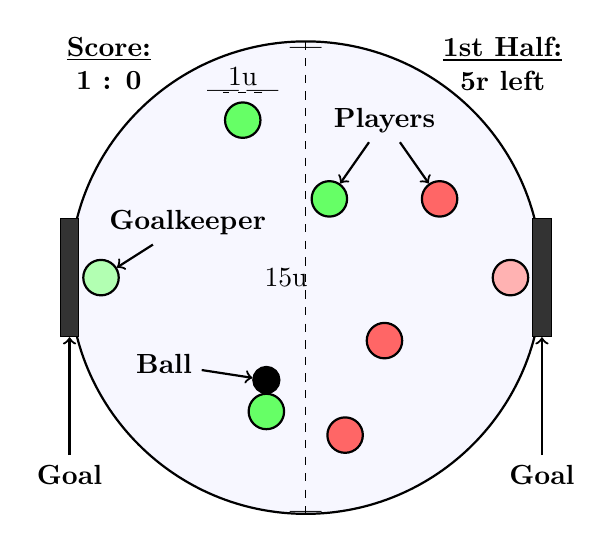
\begin{tikzpicture}[]
	\tikzstyle{test}=[thick, draw, circle, align=center]					
	\node[fill=blue!3!white, test, thick ,minimum size = 6cm](tarea)at (0,0) {};

	\node[fill=red!60!white, test,minimum size = 0.45cm](player2)at (1.7,1) {};
	\node[fill=red!60!white, test,minimum size = 0.45cm](target)at (1,-0.8) {};
	\node[fill=red!60!white, test,minimum size = 0.45cm](target)at (0.5,-2) {};

	\node[fill=green!60!white, test,minimum size = 0.45cm](target)at (-0.8,2) {};
	\node[](a1)at (-0.55,2.35) {\bf |};
	\node[](a2)at (-1.05,2.35) {\bf |};
	\node[](a2)at (-0.8,2.55) {1u};
	\draw[-, dashed](-0.55,2.35) -- (-1.05,2.35);
	
	\node[fill=green!60!white, test,minimum size = 0.45cm](player)at (0.3,1) {};
	\node[fill=green!60!white, test,minimum size = 0.45cm](target)at (-0.5,-1.7) {};
	\node[fill=black, test,minimum size = 0.1cm](ball)at (-0.5,-1.3) {};		
	\node[](tball)at (-1.8,-1.1) {\bf Ball};
	\node[](tplayer)at (1,2) {\bf Players};
	\draw[->, thick](tball) -- (ball);
	\draw[->, thick](tplayer) -- (player);
	\draw[->, thick](tplayer) -- (player2);
	
	\node[](tgk)at (-1.5,0.7) {\bf Goalkeeper};
	\node[](tgoal)at (-3,-2.5) {\bf Goal};
	\node[fill=black!80!white, draw, rectangle,minimum height=1.5cm, minimum width=0.05cm](goal)at (-3,0) {};
	\node[fill=green!30!white, test,minimum size = 0.45cm](gk)at (-2.6,0) {};
	\draw[->, thick](tgk) -- (gk);
	\draw[->, thick](tgoal) -- (goal);
	
	\node[](tgoal2)at (3,-2.5) {\bf Goal};
	\node[fill=black!80!white, draw, rectangle,minimum height=1.5cm](goal2)at (3,0) {};
	\node[fill=red!30!white, test,minimum size = 0.45cm](target)at (2.6,0) {};
	\draw[->, thick](tgoal2) -- (goal2);
	
	\node[](se2)at (0,2.9) {\bf ---};
	\node[](se2)at (0,-3) {\bf ---};
	\draw[-, dashed](0,3) -- node[] {}(0,-3);
	\node[](sca)at (-0.25,0) {15u};		
	
	\node[](sca)at (2.5,2.9) {\bf\underline{1st Half:}};
	\node[](sca)at (2.5,2.5) {\bf5r left};
	\node[](sca)at (-2.5,2.9) {\bf\underline{Score:}};
	\node[](sca)at (-2.5,2.5) {\bf 1 : 0};
	\end{tikzpicture}
	}
\end{figure}
%
\vfill
%
Each player's proficiencies in different aspects of the game are defined by the following 4 Blitzball attributes:\ofrow
\accf{Stamina Points (SP):} Represent your durability during the game. 
	Most actions cost an amount of SP to perform. 
	When your current SP reaches 0, you can keep playing, but 
	cannot perform actions that cost SP.
%
\ofrow
%
\accf{Offense (OFF):} Improves your chances of successfully passing and shooting the ball.\ofrow
\accf{Defense (DEF):} Improves your chances of stealing and intercepting the ball.\ofrow
\accf{Pace (PC):} Determines how fast you can swim.
%
\newpage
%
%\ofquote{"When you got the ball, you gotta score!"\\}{Tidus}
%
%\ofpar
%\begin{center}  \includegraphics[width=\columnwidth]{./art/blitz/stadium.jpg} \end{center}
\includegraphics[width=\columnwidth]{./art/blitz/stadium.jpg}
%
\vfill
%
During each turn, a player can swim a total distance of up to his PC+1 units and take one of the following actions.
The only exception is the goalkeeper, who stays in front of the goal at all times and only reacts to enemy shots.
The set of actions you can take changes depending on if you have the ball or not.
%
\ofrow
%
\accf{Pass:} You pass the ball to another player.
The ball can travel a maximum distance of your OFF+1d units.
While playing the pass, every opponent within 1u of you can try to block the ball.
In doing this, each blocker reduces the passes distance by their DEF+1d.
If an opponent reduces the passes distance to 0, they catch the ball.
If the ball gets past all blockers, but does not reach its target, the player closest to it
catches the ball.
%	
\ofrow
%
\accf{Shoot:} You shoot the ball on the goal. 
The ball can travel a maximum distance of your OFF+1d units.
Firstly, each shot can be blocked by nearby opponents in the same way as a pass.
Then, if the ball reaches the goal, the goalkeeper can try to catch it.
If the goalkeeper's DEF+1d is higher than the ball's remaining distance, he catches the ball,
otherwise you score a goal.
If the keeper catches the ball, he can immediately make a pass that cannot be blocked.
If you successfully score a goal, a new kick-off is performed like at the start of the game.
Each shot costs you an amount of SP equal to your OFF.
%	
\ofrow
%
\accf{Tackle:} You try to steal the ball from a player that is within 1u.
If your DEF+1d is higher than the target's DEF+1d, then you successfully steal the ball.
Also, add 1d to your roll, for each tackle that the target has suffered since his last turn.
In performing the tackle, you can additionally dash a distance of your PC+1 units.
Each tackle cost you an amount of SP equal to your DEF.
%
\ofrow
%	
\accf{Tech:}
Techs are special abilities that can help you win the game.	
Each tech contains its effect and SP cost in its description.
A list of techs is shown on the next page.
%
\vfill
%
During a Blitzball game, players may suffer the following effects for a limited duration.\ofrow
\accf{Poison:} At the start of each turn, your current SP is reduced by an amount equal to 10\% of your maximum~SP.\ofrow
\accf{Wither:} Your OFF, DEF and PC are halved.\ofrow
\accf{Nap:} Your turns are skipped and you cannot catch or block the ball.
When a player passes to you while asleep, you wake up and the ball is received by the nearest player.
%
\clearpage
%
\ofquote{"That was the Jecht shot, wasn’t it?"\\}{Yuna}\ofpar
%
\includegraphics[width=\columnwidth]{./art/blitz/ingame.jpg}
%
\ofpar
%
All blitzball attributes of a player are derived from and improved by their combat attributes as follows: \ofrow
\accf{Stamina Points = Health Points + Mana Points} \ofrow
\accf{Offense = Strength + Magic} \ofrow
\accf{Defense = (physical) Defense + Resistance} \ofrow
\accf{Pace = Agility} \ofrow
%
So if a player character levels up outside of Blitzball and gains STR+1, his OFF is also increases by 1.
To avoid confusion, Blitzball attributes should be tracked separately from combat attributes.
In the beginning each player already knows one tech of their choice.
Each player can learn up to 3 techs at most, by observing other players who perform them.
If during a game, someone within 3u of you performs a tech, you can try to pass a DC 9 check to learn it.
If you already know 3 techs, you have to forget one of them to make place for a new one.
Playing Blitzball is a source of experience for player characters, which can help them to reach adventuring milestones more quickly.
Furthermore, winners of Blitzball are usually awarded with various rewards and prices, including Equipment, Items and Gil.
%
\vfill
%
\oftable{p{0.15\columnwidth} l p{0.73\columnwidth}}
{\accf{Tech} & \accf{SP} & \accf{Effect}}
{
	Jecht Shot & 20 & You make a shot, that cannot be blocked by any player except the goalkeeper.\ofrow
	Grip Gloves & 8 & Until the start of your next turn, add 1d to your DEF while you are trying to catch a pass or shot. \ofrow
	Brawler & 8 & Until the end of your next turn, your DEF is increased by an amount equal to you OFF. \ofrow
	Aurochs Spirit & 12 & All allies within 5u increase their OFF and DEF by 3 until the start of your next turn. \ofrow
	Drain Pass & 8 & You make a pass, where you add 3u to its distance. Every player that fails to intercept it loses 5 SP and your SP is increased by the same amount. \ofrow
}
%
\newpage
%
\oftable{p{0.13\columnwidth} l p{0.73\columnwidth}}
{\accf{Tech} & \accf{SP} & \accf{Effect}}
{
%	Jecht Shot & 20 & You make a shot, that cannot be blocked by any player except the goalkeeper.\ofrow
	Sphere Shot & 15 & You make a shot, where you add 2d units to its distance.\ofrow
	Volley Shot & 6 & When you receive a pass or catch a ball before the start of your next turn, you can immediately make a shot. \ofrow
	Venom Shot & 10 & You make a shot, where you add 3u to its distance. Every player that tries to block it makes a DC 8 check and suffers Poison for 3 rounds upon failure.\ofrow
	Wither Shot & 10 & You make a shot, where you add 3u to its distance. Every player that tries to block it makes a DC 8 check and suffers Wither for 3 rounds upon failure.\ofrow
	Nap Shot & 10 & You make a shot, where you add 3u to its distance. Every player that tries to block it makes a DC 8 check and suffers Nap for 3 rounds upon failure.\ofrow
	Wither Pass & 8 & You make a pass, where you add 3u to its distance. Every player that tries to block it makes a DC 8 check and suffers Wither for 3 rounds upon failure. \ofrow
	Venom Pass & 8 & You make a pass, where you add 3u to its distance. Every player that tries to block it makes a DC 8 check and suffers Poison for 3 rounds upon failure. \ofrow
	Nap Pass & 8 & You make a pass, where you add 3u to its distance. A player that tries to block it makes a DC 8 check and suffers Nap for 3 rounds upon failure. \ofrow
	Venom Tackle & 10 & You make a tackle, where you add 3 to your usual DEF. Every player that tries to block it makes a DC 8 check and suffers Poison for 3 rounds upon failure.\ofrow
	Nap Tackle & 10 & You make a tackle, where you add 3 to your usual DEF. Every player that tries to block it makes a DC 8 check and suffers Nap for 3 rounds upon failure.\ofrow
	Wither Tackle & 10 & You make a tackle, where you add 3 to your usual DEF. Every player that tries to block it makes a DC 8 check and suffers Wither for 3 rounds upon failure. \ofrow
	Drain Tackle & 10 & You make a tackle, where you add 3 to your usual DEF. In addition, the target makes DC 8 check and upon failure his SP is reduced 5 and your SP is increased by the same amount. \ofrow
	Tackle Slip & 7 & 	Until the start of your next turn, every opponent that tries to tackle you has to make a DC 8 check first and upon failure, their tackle misses.\ofrow
	Elite \newline Defense & 8 & Until the start of your next turn, when an opponent moves within 1u of you, you can immediately make a tackle on him.\ofrow
}
%
\clearpage
\documentclass[a4paper, titlepage, 11pt, twocolumn] {article}
\usepackage{../of2}
\graphicspath{..}
%
\begin{document}
%
\ofcs{
	name=Fran, level=1,
	description={%
		\vspace*{-0.5cm}
		\begin{multicols}{2}
			Age: ?\\Gender: female\\Hair: white\\Height: 1.87m\\Eyes: brown\\quiet\\mysterious
			\columnbreak\vspace*{-1.7cm}\\
			\hspace*{0.5cm}\includegraphics[width=0.65\columnwidth]{./art/charactersheets/fran.jpg}
		\end{multicols}
		\vspace*{-0.9cm}
	},
	story={\vfill
		She grew up in a remote village hidden in the woods where she lived in harmony with nature.
		But when she become older, she left her tribe and her family behind to explore the world outside.
		\\\\
		"The Viera may begin as part of the Wood, but it is not the only end that we may choose."
	},
	hpmax=19, mpmax=17, agi=2, movement=3u, evasiondc=10, str=1, def=1, mag=0, res=1, 
	job=Marksman, abilities={Libra},
	weapon=Elfin Bow, weaponeffect=3 extra damage if target has Status, weapontype={3u Range but don't add STR to damage}, armor=Gaia Gear, armoreffect=Resilience: earth, armortype={DEF +1, RES +1},
	gil=200, inventory={\\2x Potion, 2x Antidote},
	weaponbox=\ofcsweaponboxbeginner,armorbox=\ofcsarmorboxbeginner
}
%
\ofcs{
	name=Kain, level=1,
	description={%
		\vspace*{-0.5cm}
		\begin{multicols}{2}
			Age: 21\\Gender: male\\Hair: blond\\Height: 1.83m\\ Weight: 61kg\\calm\\driven
			\columnbreak\vspace*{-1.4cm}\\
			\hspace*{-1.6cm}\includegraphics[width=1.1\columnwidth]{./art/charactersheets/kain.jpg}
		\end{multicols}
		\vspace*{-0.9cm}
	},
	story={\vfill
		Raised in a castle, he became a commander in the army like his father.
		Later, he was manipulated into betraying his lifelong friend to be with the love of his life.
		\\\\\\
		”It would seem your life is spared. For~now.”
	},
	hpmax=23, mpmax=16, agi=2, movement=3u, evasiondc=10, str=1, def=2, mag=0, res=0, 
	job=Dragoon, abilities=Jump,
	weapon=Trident, weaponeffect=Also attacks anyone right behind target, weapontype=2u range, armor=Diamond Armor, armoreffect=Resilience: lightning, armortype=DEF +2,
	gil=200, inventory={\\2x Potion\\ 1x Bomb Fragment},
	weaponbox=\ofcsweaponboxbeginner,armorbox=\ofcsarmorboxbeginner
}
%
\ofcs{
	name=Locke, level=1,
	description={%
		\vspace*{-0.5cm}
		\begin{multicols}{2}
			Age: 25\\Gender: male\\Hair: brown\\Height: 1.76m\\ Weight: 67kg\\cheerful\\ kind
			\columnbreak\vspace*{-1.7cm}\\
			\hspace*{-0.2cm}\includegraphics[width=0.7\columnwidth]{./art/charactersheets/locke.jpg}
		\end{multicols}
		\vspace*{-0.9cm}
	},
	story={\vfill
		After losing the love of his life, he has joined a rebellion group to fight against evil.
		Using his skills as a ”treasure hunter”, he worked as a spy and saboteur.\\\\\\
		”Hey! Call me a treasure hunter, or I’ll rip your lungs out!”
	},
	hpmax=20, mpmax=19, agi=4, movement=5u, evasiondc=8, str=1, def=1, mag=0, res=1, 
	job=Thief, abilities=Steal,
	weapon=Myhtril Knife, weaponeffect=Extra Materia slot, weapontype=Can wear 2nd dagger instead of accessory, armor=Myhtril Vest, armoreffect=Extra Materia slot, armortype={DEF +1, RES +1}, accessory1=Power Armlet, accessory1effect=STR+1,
	gil=150, inventory={\\2x Potion\\1x Ether},
	weaponbox=\ofcsweaponboxbeginner,armorbox=\ofcsarmorboxbeginner
}
%
\ofcs{
	name=Snow, level=1,
	description={%
		\vspace*{-0.5cm}
		\begin{multicols}{2}
			Age: 21\\Gender: male\\Hair: blonde\\Height: 2.00m\\Eyes: blue\\confident\\irresponsible
			\columnbreak\vspace*{-1.7cm}\\
			\hspace*{-0.5cm}\includegraphics[width=0.7\columnwidth]{./art/charactersheets/snow.jpg}
		\end{multicols}
		\vspace*{-0.9cm}
	},
	story={\vfill
		He is the leader of a small resistance group named NORA.
		Just after they got engaged, his fiance was cursed and turned into crystal. 
		Now he is traveling the world to find a way to lift her curse.
		\\\\\\
		"Since when have heroes ever needed plans?"
	},
	hpmax=27, mpmax=16, agi=3, movement=4u, evasiondc=9, str=1, def=2, mag=0, res=0, 
	job=Sentinel, abilities=Guard,
	weapon=Vorpal Blade, weaponeffect=Triple damage on critical hit, weapontype=counter on 11 or 12 enemy evasion check, armor=Crystal Mail, armoreffect=Resilience: ice, armortype={DEF +2},
	gil=200, inventory={\\1x Potion, 1x Lunar Curtain},
	weaponbox=\ofcsweaponboxbeginner,armorbox=\ofcsarmorboxbeginner
}
%
\ofcs{
	name=Squall, level=1,
	description={%
		\vspace*{-0.5cm}
		\begin{multicols}{2}
			Age: 17\\Gender: male\\Hair: brown\\Height: 1.75m\\ Right-Handed\\introvered\\aloof
			\columnbreak\vspace*{-1.7cm}\\
			\hspace*{-0.6cm}\includegraphics[width=0.9\columnwidth]{./art/charactersheets/squall.jpg}
		\end{multicols}
		\vspace*{-0.9cm}
	},
	story={\vfill
		Grew up in an orphanage after his parents died.
		Then, he was trained in an academy to become a talented mercenary who has mastered the gunblade.
		A lone wolf, without many friends.\\\\
		”Why do people depend on each other? In the end, you are on your own.”
	},
	hpmax=25, mpmax=18, agi=3, movement=4u, evasiondc=9, str=1, def=1, mag=0, res=1, 
	job=Warrior, abilities=Rush,
	weapon=Gunblade, weaponeffect=Ranged attack after ability, weapontype=counter on 11 or 12 enemy evasion check, armor=Myhtril Vest, armoreffect=Extra Materia slot, armortype={DEF +1, RES +1},
	gil=250, inventory={\\2x Potion, 2x Eyedrops, 1x Giant's Tonic},
	weaponbox=\ofcsweaponboxbeginner,armorbox=\ofcsarmorboxbeginner
}
%
\ofcs{
	name=Tifa, level=1,
	description={%
		\vspace*{-0.5cm}
		\begin{multicols}{2}
			Age: 20\\Gender: fem.\\Hair: dark\\Height: 1.67m\\Eyes: brown\\empathic\\reserved
			\columnbreak\vspace*{-1.7cm}\\
			\hspace*{0.2cm}\includegraphics[width=0.6\columnwidth]{./art/charactersheets/tifa.jpg}
		\end{multicols}
		\vspace*{-0.9cm}
	},
	story={\vfill
		Grew up in a village where she was trained by a master of martial arts.
		After the destruction of her village and the death of her family, she moved to a big city 
		and joined an environmentalist resistance group.
		\\\\
		”Words aren't the only way to tell someone how you feel.”
	},
	hpmax=20, mpmax=16, agi=4, movement=5u, evasiondc=8, str=2, def=1, mag=0, res=1, 
	job=Monk, specials=Brawler,
	weapon=Power Armlet, weaponeffect=STR+1, armor=Kenpo Gi, armoreffect=Immunity: Blind, armortype={DEF +1, RES +1},
	gil=200, inventory={\\3x Potion},
	weaponbox=\ofcsweaponboxbeginner,armorbox=\ofcsarmorboxbeginner
}
%
\ofcs{
	name=Vivi, level=1,
	description={%
		\vspace*{-0.5cm}
		\begin{multicols}{2}
			Age: 9\\Gender: male\\Race: ?\\Height: 1.21m\\ Right-Handed\\shy\\clumsy
			\columnbreak\vspace*{-1.7cm}\\
			\hspace*{-0.3cm}\includegraphics[width=0.7\columnwidth]{./art/charactersheets/vivi.jpg}
		\end{multicols}
		\vspace*{-0.9cm}
	},
	story={\vfill
		Fell off a cargo ship and was found by a gourmand named Quan, who he sees as his grandfather. 
		Lived in his cave for a few months until Quan died. 
		When alone, he left to find out more about his past.
		\\\\
	 	”I have to find out who I am. I’m scared. What if I’m not even human?”
	},
	hpmax=18, mpmax=26, agi=2, movement=3u, evasiondc=10, str=0, def=0, mag=2, res=3, 
	job=Black Mage, abilities={Fire, Blizzard, Thunder},
	weapon=Stardust Rod, weaponeffect=Regain MP equal to Level on enemy KO, weapontype=MAG +2, armor=Myhtril Robe, armoreffect=Extra Materia slot, armortype=RES +2,
	gil=250, inventory={\\2x Potion\\2x Ether},
	weaponbox=\ofcsweaponboxbeginner,armorbox=\ofcsarmorboxbeginner
}
%
\ofcs{
	name=Yuna, level=1,
	description={%
		\vspace*{-0.5cm}
		\begin{multicols}{2}
			Age: 17\\Gender: fem.\\Hair: brown\\Height: 1.60m\\Heterochromia\\honest\\passionate
			\columnbreak\vspace*{-1.7cm}\\
			\hspace*{0.5cm}\includegraphics[width=0.4\columnwidth]{./art/charactersheets/yuna.jpg}
		\end{multicols}
		\vspace*{-0.9cm}
	},
	story={\vfill
		Her parents died at a young age and she was raised in a remote village. 
		Her father was a famous high summoner, who sacrificed himself to bring peace. 
		She wants to walk in his footsteps to continue his legacy.\\\\
		”I will defeat sorrow, in his place.”
	},
	hpmax=16, mpmax=34, agi=2, movement=3u, evasiondc=10, str=1, def=0, mag=0, res=2, 
	job=Summoner, abilities={Summon (Carbuncle)},
	weapon=Myhtril Staff, weaponeffect=Extra Materia slot, weapontype=Maximum MP +10, armor=White Robe, armoreffect=Immunity: Sleep, armortype=RES +2,
	gil=200, inventory={\\3x Potion\\ 1x Remedy},
	weaponbox=\ofcsweaponboxbeginner,armorbox=\ofcsarmorboxbeginner
}
%
\end{document}
%
\end{document}